\documentclass[11pt,a4paper,twoside]{book}
\usepackage[T1]{fontenc}
\usepackage[utf8]{inputenc}
\usepackage{mathpazo}
\usepackage[scaled=0.90]{helvet}
\usepackage{courier}
\usepackage[a4paper,inner=3.0cm,outer=2.4cm,top=2.6cm,bottom=2.8cm]{geometry}
\usepackage{xcolor}
\usepackage{mathtools}
\usepackage{colortbl}
\usepackage{tikz}
\usetikzlibrary{calc,positioning,arrows.meta,decorations.pathmorphing}
\usepackage{booktabs}
\usepackage{array}
\usepackage{longtable}
\usepackage{enumitem}
\usepackage[german=quotes]{csquotes}
\usepackage{fancyhdr}
\usepackage{titlesec}
\usepackage{amsmath,amssymb}
\usepackage{emptypage}
\usepackage{tcolorbox}
\tcbuselibrary{skins,breakable}
\usepackage[hidelinks]{hyperref}

\definecolor{tief}{HTML}{1F3A5F}
\definecolor{mittel}{HTML}{2E5F8A}
\definecolor{akzent}{HTML}{A34A28}
\definecolor{sand}{HTML}{F4F1EA}
\definecolor{grau}{HTML}{5A5A5A}
\definecolor{gruen}{HTML}{2F6B4F}
\definecolor{purpur}{HTML}{5B3A72}

\newcolumntype{P}[1]{>{\raggedright\arraybackslash}p{#1}}

\newcommand{\kursiv}[1]{{\itshape\color{grau}#1}}
\newcommand{\code}[1]{{\ttfamily\small #1}}
\newcommand{\Person}[1]{\textbf{#1}}
\newcommand{\Begriff}[1]{\textbf{#1}}
\newcommand{\zit}[1]{\textsuperscript{[#1]}}
\newcommand{\Oh}{\mathcal{O}}
\newcommand{\boxtitel}[1]{{\bfseries\color{tief}#1}\par\nopagebreak\vspace{6pt}\nopagebreak}
\newcommand{\boxtitelr}[1]{{\bfseries\color{akzent}#1}\par\nopagebreak\vspace{6pt}\nopagebreak}
\newcommand{\boxtitelg}[1]{{\bfseries\color{gruen}#1}\par\nopagebreak\vspace{6pt}\nopagebreak}
\newcommand{\boxtitelp}[1]{{\bfseries\color{purpur}#1}\par\nopagebreak\vspace{6pt}\nopagebreak}
\newcommand{\boxtitelm}[1]{{\bfseries\color{mittel}#1}\par\nopagebreak\vspace{6pt}\nopagebreak}
\newcommand{\loesung}{\par\vspace{8pt}{\bfseries\color{mittel}Lösung}\par\nopagebreak\vspace{4pt}\nopagebreak}
\newcommand{\schritt}[1]{\par\vspace{5pt}{\bfseries\color{grau}#1}\par\nopagebreak\vspace{2pt}\nopagebreak}

% Graphentheoretische Notation
\newcommand{\Gr}{G}
\newcommand{\Kn}[1]{K_{#1}}
\newcommand{\Kmn}[2]{K_{#1,#2}}
\newcommand{\Grad}{\deg}
\newcommand{\Nb}{N}
\newcommand{\chrom}{\chi}
\newcommand{\Ecken}{V}
\newcommand{\Kanten}{E}

\newtcolorbox{grundbox}[1][tief]{
  breakable, enhanced, colback=sand, colframe=sand,
  boxrule=0pt, leftrule=3pt, borderline west={3pt}{0pt}{#1},
  left=12pt, right=10pt, top=10pt, bottom=10pt,
  sharp corners, before skip=12pt, after skip=12pt, shrink break goal=24pt}

\newenvironment{merksatz}{\begin{grundbox}[tief]}{\end{grundbox}}
\newenvironment{warnung}{\begin{grundbox}[akzent]}{\end{grundbox}}
\newenvironment{definition}{\begin{grundbox}[mittel]}{\end{grundbox}}
\newenvironment{geschichte}{\begin{grundbox}[gruen]}{\end{grundbox}}
\newenvironment{forschung}{\begin{grundbox}[purpur]}{\end{grundbox}}
\newenvironment{aufgabe}{\begin{grundbox}[grau]}{\end{grundbox}}
\newenvironment{technik}{\begin{grundbox}[mittel]}{\end{grundbox}}

\titleformat{\chapter}[display]
  {\normalfont\huge\bfseries\color{tief}}{\Large\color{grau}Kapitel \thechapter}{8pt}{\Huge}
\titleformat{\part}[display]
  {\normalfont\huge\bfseries\color{tief}\filcenter}{\Large\color{grau}Teil \thepart}{10pt}{\Huge}
\titlespacing*{\chapter}{0pt}{10pt}{28pt}

\pagestyle{fancy}
\fancyhf{}
\fancyhead[LE,LO]{\small\itshape\color{grau}\leftmark}
\fancyfoot[LE,LO]{\small\color{grau}\thepage}
\renewcommand{\headrulewidth}{0.4pt}
\renewcommand{\footrulewidth}{0pt}
\renewcommand{\chaptermark}[1]{\markboth{#1}{}}
\setlength{\parindent}{0pt}
\setlength{\parskip}{6pt}
\renewcommand{\arraystretch}{1.3}

\renewcommand{\contentsname}{Inhaltsverzeichnis}
\renewcommand{\chaptername}{Kapitel}
\renewcommand{\partname}{Teil}
\renewcommand{\appendixname}{Anhang}
\renewcommand{\tablename}{Tabelle}
\renewcommand{\figurename}{Abbildung}

\hyphenation{Si-mu-la-ti-on Zu-falls-zah-len Pseu-do-zu-fall Ver-wer-fungs-me-tho-de
Mon-te-Car-lo Va-ri-anz-re-duk-ti-on Dis-kre-ti-sie-rung Schritt-wei-te
Er-eig-nis-si-mu-la-ti-on Ab-wei-sungs-ra-te Ein-schwing-pha-se
Öko-no-me-trie öko-no-me-trisch En-do-ge-ni-tät
In-stru-ment-va-ri-a-ble Si-mul-ta-ni-tät Iden-ti-fi-ka-ti-on Pa-nel-da-ten
Ko-in-te-gra-ti-on Ein-heits-wur-zel Vek-tor-au-to-re-gres-si-on
Zu-zah-lung Arzt-be-su-che Preis-elas-ti-zi-tät Mo-men-ten-me-tho-de
Ir-rfahrt Mar-kow-Ket-te Über-gangs-ma-trix sta-tio-när
Brown-sche Brown-schen Mar-tin-gal Mar-tin-ga-le Stopp-zeit Stopp-zei-ten
Pois-son-Pro-zess Ver-zwei-gungs-pro-zess Fil-tra-ti-on Pfad-ei-gen-schaft
Dif-fu-si-on Dif-fu-si-o-nen Wie-ner-Pro-zess Ar-kus-si-nus-Ge-setz
Ent-schei-dung Ent-schei-dun-gen Nut-zen-funk-ti-on Ri-si-ko-aver-si-on
An-ti-ko-agu-la-ti-on Vor-hof-flim-mern Schlag-an-fall Blu-tungs-ri-si-ko
Er-war-tungs-nut-zen Si-cher-heits-äqui-va-lent Ent-schei-dungs-baum
Schwel-len-wert Mar-kow-Mo-dell Dis-kon-tie-rung Prio-ri-sie-rung
Kau-sa-li-tät kau-sa-le kau-sa-len Stör-grö-ße Stör-grö-ßen Kol-li-der
Me-di-a-tor Me-di-a-ti-on Hin-ter-tür-test Rando-mi-sie-rung rando-mi-siert
In-stru-ment-va-ri-a-ble Ziel-stu-di-en-emu-la-ti-on Stan-dar-di-sie-rung
Kon-tra-fak-tisch kon-tra-fak-ti-sche Be-hand-lungs-ef-fekt Neu-stadt Kli-ni-kum
Sep-sis An-ti-bio-ti-ka-ga-be Be-ob-ach-tungs-da-ten Be-ob-ach-tungs-äqui-va-lenz
Pro-pen-si-ty Ge-wich-tung Schwe-re-grad}

\tikzset{
  knoten/.style={circle, fill=tief, inner sep=0pt, minimum size=5.5pt},
  knotenb/.style={circle, draw=tief, fill=white, line width=0.9pt, inner sep=1pt, minimum size=15pt, font=\scriptsize},
  knotenr/.style={circle, draw=akzent, fill=akzent!12, line width=0.9pt, inner sep=1pt, minimum size=15pt, font=\scriptsize},
  knoteng/.style={circle, draw=gruen, fill=gruen!12, line width=0.9pt, inner sep=1pt, minimum size=15pt, font=\scriptsize},
  kante/.style={draw=grau, line width=0.9pt},
  kanted/.style={draw=akzent, line width=1.5pt},
}

\newcommand{\MW}{\overline{x}}
\newcommand{\dd}{\mathrm{d}}
\newcommand{\R}{\mathbb{R}}
\newcommand{\Z}{\mathbb{Z}}
\newcommand{\Ent}{H}
\newcommand{\vek}[1]{\boldsymbol{#1}}
\newcommand{\lb}{\operatorname{ld}}



\newcommand{\Risk}{\mathcal{R}}
\newcommand{\Hyp}{\mathcal{H}}
\newcommand{\E}{\mathbb{E}}

\newcommand{\dops}{\operatorname{do}}



\begin{document}
\frontmatter
\begin{titlepage}
\centering
\vspace*{1.6cm}
{\footnotesize\scshape\color{grau} Mathematik von Grund auf --- Band 29}\\[2.0cm]
{\Huge\bfseries\color{tief} Die Form\\[6pt] der Lösungen}\\[16pt]
{\Large\color{akzent} Algebraische Geometrie}\\[1.5cm]

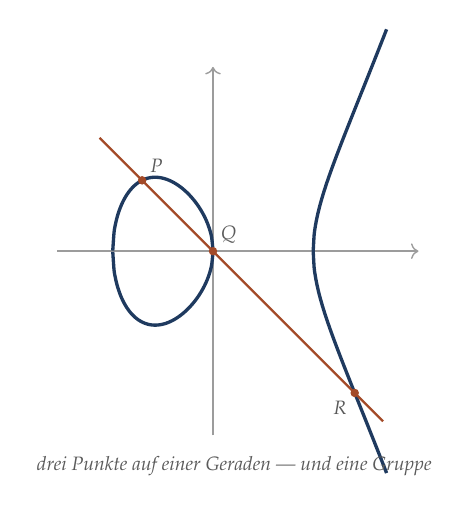
\begin{tikzpicture}[scale=0.9]
% Die Kurve y^2 = x^3 - 2x mit Sekante durch P=(-1,1), Q=(0,0): dritter Schnittpunkt R=(2,-2)
\draw[grau!60, line width=0.5pt, ->] (-2.2,0) -- (2.9,0);
\draw[grau!60, line width=0.5pt, ->] (0,-2.6) -- (0,2.6);
\draw[tief, line width=1.2pt, domain=-1.4142:0, samples=80, smooth] plot (\x, {sqrt(max(0,\x*\x*\x-2*\x))});
\draw[tief, line width=1.2pt, domain=-1.4142:0, samples=80, smooth] plot (\x, {-sqrt(max(0,\x*\x*\x-2*\x))});
\draw[tief, line width=1.2pt, domain=1.4142:2.45, samples=80, smooth] plot (\x, {sqrt(max(0,\x*\x*\x-2*\x))});
\draw[tief, line width=1.2pt, domain=1.4142:2.45, samples=80, smooth] plot (\x, {-sqrt(max(0,\x*\x*\x-2*\x))});
\draw[akzent, line width=0.8pt] (-1.6,1.6) -- (2.4,-2.4);
\fill[akzent] (-1,1) circle (1.7pt) node[above right=-1pt, font=\scriptsize, color=grau] {$P$};
\fill[akzent] (0,0) circle (1.7pt) node[above right=-1pt, font=\scriptsize, color=grau] {$Q$};
\fill[akzent] (2,-2) circle (1.7pt) node[below left=-1pt, font=\scriptsize, color=grau] {$R$};
\node[font=\scriptsize\itshape, color=grau, anchor=north] at (0.3,-2.75) {drei Punkte auf einer Geraden --- und eine Gruppe};
\end{tikzpicture}

\vspace{1.4cm}
{\large\color{grau} Von der Nullstellenmenge bis zur Kurve mit Gruppengesetz}\\[6pt]
{\color{grau} Jeder Schritt erklärt. Mit vollständig durchgerechneten Übungsaufgaben.}\\[1.9cm]
{\small\color{grau} Stand der Forschung: August 2026}
\end{titlepage}
\thispagestyle{empty}
\vspace*{\fill}
\begin{flushleft}
{\small\color{grau}
\textbf{\color{tief}Mathematik von Grund auf} --- Band 29\\[2pt]
\textit{Die Form der Lösungen} $\cdot$ Algebraische Geometrie\\[14pt]

Herausgeber und Urheber: Jürgen Maier\\[2pt]
Entstanden 2026 in Zusammenarbeit mit Claude (Anthropic); Konzeption, Vorgaben, Prüfung und Herausgeberschaft: Jürgen Maier.\\[14pt]

\textbf{Lizenz}\\[2pt]
Dieses Werk ist lizenziert unter einer Creative-Commons-Lizenz \textbf{Namensnennung -- Weitergabe unter gleichen Bedingungen 4.0 International (CC BY-SA 4.0)}. Sie dürfen das Werk vervielfältigen, verbreiten, bearbeiten und auch kommerziell nutzen, sofern Sie den Urheber nennen und Bearbeitungen unter derselben Lizenz weitergeben.\\[2pt]
Lizenztext: \texttt{https://creativecommons.org/licenses/by-sa/4.0/legalcode.de}\\[14pt]

\textbf{Quellen und Fassungen}\\[2pt]
Quelltexte, Simulationen, Fehlermeldungen und aktuelle Fassungen aller Bände:\\
\texttt{https://github.com/juergenmaier2026/mathematik-von-grund-auf}\\[2pt]
Dauerhaft archiviert bei Zenodo: \texttt{https://doi.org/10.5281/zenodo.23698547}\\[14pt]

\textbf{Zitiervorschlag}\\[2pt]
Maier, J. (2026). \textit{Mathematik von Grund auf, Band 29: Die Form der Lösungen}. Fassung 1.1.0. \texttt{https://doi.org/10.5281/zenodo.23698547}\\[14pt]

Satz: \LaTeX{} mit Palatino. Fassung 1.1.0, Oktober 2026. 188 Seiten.
}
\end{flushleft}
\vspace*{1.5cm}

\tableofcontents
\mainmatter

\chapter*{Vorwort}
\addcontentsline{toc}{chapter}{Vorwort}

\section*{Worum es geht}

\begin{merksatz}
\boxtitel{Ein Medikament, zwei Kammern, vier Zahlen}
Ein Wirkstoff wird in die Blutbahn gespritzt, verteilt sich ins Gewebe und zurück, und wird ausgeschieden. Das einfachste Modell hat zwei Kammern und vier Geschwindigkeiten: $k_{12}$ (Blut ins Gewebe), $k_{21}$ (zurück), $k_{10}$ (Ausscheidung aus dem Blut), $k_{20}$ (Ausscheidung aus dem Gewebe). Gemessen wird nur die Konzentration im Blut, und sie fällt als Summe zweier Exponentialfunktionen.

\begin{center}
{\small
\renewcommand{\arraystretch}{1.5}
\begin{tabular}{@{}P{3.6cm}P{5.0cm}@{}}
\toprule
\textbf{Was die Messung liefert} & drei Zahlen: $s_1 = k_{10} + k_{12}$, $s_2 = k_{10} + k_{12} + k_{21} + k_{20}$, $s_3 = k_{10}k_{21} + k_{10}k_{20} + k_{12}k_{20}$\\
\textbf{Was man wissen will} & vier Zahlen: $k_{10}, k_{12}, k_{21}, k_{20}$\\
\textbf{Die Frage} & Welche Parametersätze passen zu denselben Daten? Einer, endlich viele, unendlich viele?\\
\bottomrule
\end{tabular}}
\end{center}

\begin{center}
\begin{minipage}{0.9\textwidth}
\textbf{Die Antwort ist eine Nullstellenmenge: alle $(k_{10}, k_{12}, k_{21}, k_{20})$, die drei polynomiale Gleichungen erfüllen. Ihre Gestalt --- Punkt, Punktepaar, Kurve --- ist die Antwort auf die Frage, ob das Modell aus den Daten bestimmbar ist. Für vier Parameter ist sie eine Kurve: unendlich viele Modelle, dieselben Daten.}
\end{minipage}
\end{center}

\begin{center}
\begin{minipage}{0.88\textwidth}
\kursiv{\textbf{Algebraische Geometrie ist die Lehre von den Lösungsmengen polynomialer Gleichungen} --- ihrer Gestalt, ihrer Dimension, ihrer Zerlegung in Teile, ihrer Schnittpunkte. Dieses Buch nimmt den Weg von der Nullstellenmenge zur Kurve mit Gruppengesetz und hält an jedem Schritt an einem Beispiel an, das man durchrechnen kann. Der Leitfall --- die Frage, ob ein Modell aus Daten bestimmbar ist --- begleitet den Band, weil er genau die Werkzeuge braucht, die er entwickelt: Ideale, Gröbner-Basen, Elimination, Dimension. Und weil er zeigt, dass eine Frage der Medizin eine Frage der Geometrie sein kann, ohne dass jemand etwas zeichnet.}
\end{minipage}
\end{center}
\end{merksatz}

\section*{Drei Überraschungen}

\begin{merksatz}
\boxtitel{Was dieser Band zeigt}
\begin{center}
{\small
\renewcommand{\arraystretch}{1.5}
\begin{tabular}{@{}P{0.5cm}P{8.2cm}@{}}
\toprule
$1$ & Unendlich viele polynomiale Gleichungen in endlich vielen Unbekannten haben immer dieselbe Lösungsmenge wie endlich viele von ihnen --- und man kann die endlich vielen ausrechnen. \kursiv{(Kapitel 2 und 5)}\\
$2$ & Zwei ebene Kurven der Grade $m$ und $n$ schneiden sich in genau $mn$ Punkten --- wenn man richtig zählt: mit Vielfachheit, im Komplexen und im Unendlichen. \kursiv{(Kapitel 9)}\\
$3$ & Die Punkte einer Kurve dritten Grades bilden eine Gruppe: Man kann sie addieren, und die Addition ist die Grundlage der Verschlüsselung in jedem Mobiltelefon. \kursiv{(Kapitel 10)}\\
\bottomrule
\end{tabular}}
\end{center}

\begin{center}
\begin{minipage}{0.88\textwidth}
\kursiv{Die erste Überraschung ist Hilberts Basissatz von 1890, die zweite Bézouts Satz von 1779, die dritte eine Entdeckung, die sich über zweihundert Jahre von Fermat bis Poincaré hinzog. Alle drei werden in diesem Band bewiesen --- die erste vollständig, die zweite bis auf die Vielfachheitstheorie, die dritte mit dem Gruppengesetz in Koordinaten, das man nachrechnen kann.}
\end{minipage}
\end{center}
\end{merksatz}

\section*{Der Aufbau}

\begin{merksatz}
\boxtitel{Die sechs Teile}
\begin{center}
{\small
\renewcommand{\arraystretch}{1.5}
\begin{tabular}{@{}P{1.4cm}P{3.6cm}P{3.0cm}@{}}
\toprule
\textbf{Teil} & \textbf{Thema} & \textbf{Kapitel}\\
\midrule
I & Nullstellen und Ideale & $1$--$3$\\
II & Rechnen mit Idealen & $4$--$6$\\
III & Die Gestalt & $7$--$9$\\
IV & Kurven & $10$--$12$\\
V & Anwendungen & $13$--$14$\\
VI & Stand & $15$\\
\bottomrule
\end{tabular}}
\end{center}

\schritt{Was vorausgesetzt wird}
Ringe, Ideale und Körper in dem Umfang von Band 11 (Algebra); lineare Algebra mit Determinanten und Rang (Band 2); die komplexen Zahlen und der Fundamentalsatz der Algebra (Band 12). Für Kapitel 10 und 14 ist Band 1 (Zahlentheorie) nützlich, für den Leitfall Band 18 (Kompartimentmodelle) und Band 26 (Identifizierbarkeit), aber nicht nötig. Alles andere wird hier entwickelt, und wo ein Beweis übergangen wird, steht es dabei --- die Auslassungen sind im Anhang gesammelt.

\begin{center}
\begin{minipage}{0.88\textwidth}
\kursiv{\textbf{Jedes Kapitel endet mit einem Bruchfall}: einem Beispiel, an dem die Methode des Kapitels versagt --- die reelle Zeichnung, die die Varietät nicht zeigt; die Gröbner-Basis, die zu groß wird; der Satz von Bézout ohne Vielfachheit. Und jedes Kapitel hat drei Übungsaufgaben mit vollständiger Lösung und Probe. Die Gröbner-Basen in diesem Band wurden mit einem Programm von gut hundert Zeilen gerechnet, das der Leser nach Kapitel 5 selbst schreiben kann; es liegt den Quellen bei.}
\end{minipage}
\end{center}
\end{merksatz}

\part{Nullstellen und Ideale}

\chapter{Was eine Gleichung zeichnet}

\section{Die Lösungsmenge als Gegenstand}

\begin{merksatz}
\boxtitel{Drei Gleichungen, vier Unbekannte, eine Kurve}
Für den Leitfall mit gemessenen Werten $s_1 = \tfrac12$, $s_2 = \tfrac{9}{10}$, $s_3 = \tfrac{14}{100}$ lauten die Gleichungen
\[ k_{10} + k_{12} = \tfrac12, \qquad k_{10} + k_{12} + k_{21} + k_{20} = \tfrac{9}{10}, \qquad k_{10}k_{21} + k_{10}k_{20} + k_{12}k_{20} = \tfrac{14}{100} . \]
Aus den ersten beiden: $k_{10} = \tfrac12 - k_{12}$ und $k_{21} = \tfrac{2}{5} - k_{20}$. Einsetzen in die dritte:
\[ \bigl(\tfrac12 - k_{12}\bigr)\bigl(\tfrac25 - k_{20}\bigr) + \bigl(\tfrac12 - k_{12}\bigr)k_{20} + k_{12}k_{20} = \tfrac15 - \tfrac25 k_{12} + k_{12}k_{20} = \tfrac{14}{100}, \]
also $k_{12}k_{20} - \tfrac25 k_{12} + \tfrac{3}{50} = 0$, oder $k_{20} = \tfrac25 - \dfrac{3}{50\,k_{12}}$.

\begin{center}
{\small
\renewcommand{\arraystretch}{1.46}
\begin{tabular}{@{}P{1.4cm}P{1.4cm}P{1.4cm}P{1.4cm}P{2.6cm}@{}}
\toprule
$k_{12}$ & $k_{10}$ & $k_{20}$ & $k_{21}$ & \textbf{Deutung}\\
\midrule
$0{,}15$ & $0{,}35$ & $0{,}00$ & $0{,}40$ & keine Ausscheidung aus dem Gewebe\\
$0{,}20$ & $0{,}30$ & $0{,}10$ & $0{,}30$ & die \enquote{wahren} Werte\\
$0{,}30$ & $0{,}20$ & $0{,}20$ & $0{,}20$ & gleiche Ausscheidung beiderseits\\
$0{,}50$ & $0{,}00$ & $0{,}28$ & $0{,}12$ & keine Ausscheidung aus dem Blut\\
\bottomrule
\end{tabular}}
\end{center}

\begin{center}
\begin{minipage}{0.9\textwidth}
\textbf{Jede Zeile ist ein Modell, und alle vier erzeugen exakt dieselbe Blutkurve. Die Lösungsmenge ist eine Kurve im vierdimensionalen Parameterraum --- ein Hyperbelast, parametrisiert durch $k_{12}\in[0{,}15;\ 0{,}5]$. Die Daten sagen nicht, wo auf ihr das Medikament liegt.}
\end{minipage}
\end{center}

\begin{center}
\begin{minipage}{0.88\textwidth}
\kursiv{\textbf{Das Rechnen war hier leicht, weil zwei der drei Gleichungen linear waren.} Mit drei Kammern, oder mit einer Messung im Gewebe statt im Blut, oder mit nichtlinearer Ausscheidung sind alle Gleichungen vom Grad zwei oder höher, und das Einsetzen führt in ein Dickicht. Dieses Buch ersetzt das Einsetzen durch eine Theorie: Die Lösungsmenge wird zum Gegenstand, mit Dimension, Bestandteilen und Gleichungen, die man systematisch vereinfachen kann. Die Kurve des Leitfalls hat Dimension eins --- das ist der Satz \enquote{nicht identifizierbar} in der Sprache dieses Bandes, und Kapitel 7 sagt, wie man die Dimension berechnet, ohne die Kurve zu finden.}
\end{minipage}
\end{center}
\end{merksatz}

\section{Affine Varietäten}

\begin{definition}
\boxtitelm{Definition 1.1 --- affine Varietät}
Sei $k$ ein Körper und $k[x_1, \ldots, x_n]$ der Ring der Polynome in $n$ Veränderlichen. Für Polynome $f_1, \ldots, f_s$ heißt
\[ V(f_1, \ldots, f_s) = \{\,a \in k^{n} : f_1(a) = \cdots = f_s(a) = 0\,\} \]
die von ihnen bestimmte \Begriff{affine Varietät}. Der Raum $k^{n}$ heißt \Begriff{affiner Raum} $\mathbb A^{n}$; der Körper ist in diesem Band meist $\mathbb Q$, $\mathbb R$ oder $\mathbb C$, in Kapitel 10 und 14 auch ein endlicher Körper $\mathbb F_p$.
\end{definition}

\begin{merksatz}
\boxtitel{Beispiele, die wiederkommen}
\begin{center}
{\small
\renewcommand{\arraystretch}{1.5}
\begin{tabular}{@{}P{3.6cm}P{5.0cm}@{}}
\toprule
$V(x^{2} + y^{2} - 1)\subset\mathbb R^{2}$ & der Einheitskreis: eine Kurve\\
$V(y - x^{2})$ & die Parabel\\
$V(y^{2} - x^{3} + 2x)$ & eine Kubik mit zwei Ästen (Titelbild)\\
$V(y^{2} - x^{3})$ & die Neilsche Parabel mit Spitze im Ursprung\\
$V(y^{2} - x^{2}(x+1))$ & ein Blatt, das sich im Ursprung kreuzt\\
$V(y - x^{2},\ z - x^{3})\subset\mathbb R^{3}$ & die verdrehte Kubik $(t, t^{2}, t^{3})$: eine Raumkurve\\
$V(xz,\ yz)$ & die $xy$-Ebene vereinigt mit der $z$-Achse\\
$V(x^{2} + y^{2})\subset\mathbb R^{2}$ & ein Punkt --- aber in $\mathbb C^{2}$ zwei Geraden\\
$V(1)$, $V(0)$ & leer; der ganze Raum\\
\bottomrule
\end{tabular}}
\end{center}

\begin{center}
\begin{minipage}{0.9\textwidth}
\textbf{Eine Gleichung in der Ebene gibt gewöhnlich eine Kurve, zwei Gleichungen im Raum eine Kurve, eine Gleichung im Raum eine Fläche. Aber nicht immer: $V(xz, yz)$ hat Teile verschiedener Dimension, und $V(x^{2}+y^{2})$ hängt vom Körper ab.}
\end{minipage}
\end{center}
\end{merksatz}

\begin{merksatz}
\boxtitel{Satz 1.2 --- Varietäten lassen sich schneiden und vereinigen}
Sind $V = V(f_1, \ldots, f_s)$ und $W = V(g_1, \ldots, g_t)$ affine Varietäten in $k^{n}$, so auch
\[ V\cap W = V(f_1, \ldots, f_s, g_1, \ldots, g_t) \qquad\text{und}\qquad V\cup W = V(f_ig_j : 1\le i\le s,\ 1\le j\le t). \]

\schritt{Beweis für den Durchschnitt}
$a\in V\cap W$ genau dann, wenn alle $f_i(a) = 0$ und alle $g_j(a) = 0$ --- das ist die Definition der rechten Seite. $\blacksquare$

\schritt{Beweis für die Vereinigung}
Ist $a\in V$, so sind alle $f_i(a) = 0$, also alle Produkte $f_i(a)g_j(a) = 0$: $a$ liegt rechts. Ebenso für $a\in W$. Umgekehrt: Liegt $a$ rechts und nicht in $V$, so ist ein $f_{i_0}(a)\ne0$; aus $f_{i_0}(a)g_j(a) = 0$ für alle $j$ folgt dann $g_j(a) = 0$ für alle $j$, also $a\in W$. $\blacksquare$

\schritt{Beispiel}
$V(xz, yz) = V(x, y)\cup V(z)$: die $z$-Achse ($x = y = 0$) vereinigt mit der $xy$-Ebene ($z = 0$). Die Produkte $x\cdot z$ und $y\cdot z$ sind genau die Gleichungen. \checkmark

\begin{center}
\begin{minipage}{0.88\textwidth}
\kursiv{\textbf{Der Satz sagt, dass die Varietäten die abgeschlossenen Mengen einer Topologie bilden} --- der Zariski-Topologie, Band 8 ---, in der endliche Vereinigungen und beliebige Durchschnitte abgeschlossener Mengen abgeschlossen sind. Es ist eine seltsame Topologie: Jede nichtleere offene Menge der Geraden ist das Komplement endlich vieler Punkte, zwei offene Mengen schneiden sich immer. Aber sie ist die richtige für Polynome, weil sie nur das sieht, was Polynome sehen. Die Vereinigung in Satz 1.2 ist der Grund, warum Varietäten in Bestandteile zerfallen (Kapitel 3): $V(xz, yz)$ ist nicht \enquote{ein} Gebilde, sondern zwei.}
\end{minipage}
\end{center}
\end{merksatz}

\section{Parametrisierungen}

\begin{merksatz}
\boxtitel{Satz 1.3 --- von der Parametrisierung zur Gleichung, und zurück}
Zwei Arten, eine Varietät zu beschreiben:
\begin{center}
{\small
\renewcommand{\arraystretch}{1.5}
\begin{tabular}{@{}P{2.4cm}P{3.0cm}P{3.2cm}@{}}
\toprule
 & \textbf{implizit} & \textbf{parametrisch}\\
\midrule
Form & $f_1 = \cdots = f_s = 0$ & $x_i = g_i(t_1, \ldots, t_m)$\\
gut für & prüfen, ob ein Punkt dazugehört & Punkte erzeugen, zeichnen\\
Beispiel Kreis & $x^{2} + y^{2} = 1$ & $x = \frac{1-t^{2}}{1+t^{2}},\ y = \frac{2t}{1+t^{2}}$\\
\bottomrule
\end{tabular}}
\end{center}
Jede polynomiale (oder rationale) Parametrisierung beschreibt eine Teilmenge einer affinen Varietät, und die kleinste Varietät, die sie enthält, lässt sich berechnen (\Begriff{Implizitisierung}, Kapitel 6). Nicht jede Varietät hat eine Parametrisierung (Kapitel 12).

\schritt{Der Kreis, nachgerechnet}
$x^{2} + y^{2} = \dfrac{(1-t^{2})^{2} + 4t^{2}}{(1+t^{2})^{2}} = \dfrac{1 + 2t^{2} + t^{4}}{(1+t^{2})^{2}} = 1$. \checkmark\ Die Parametrisierung trifft jeden Punkt des Kreises außer $(-1, 0)$: Der wäre $t = \infty$.

\schritt{Die verdrehte Kubik}
$(t, t^{2}, t^{3})$ erfüllt $y = x^{2}$ und $z = x^{3}$; umgekehrt gibt jeder Punkt von $V(y - x^{2}, z - x^{3})$ mit $t = x$ eine Parameterdarstellung. Hier stimmen Bild und Varietät überein.

\begin{center}
\begin{minipage}{0.9\textwidth}
\textbf{Der Leitfall ist implizit gegeben (drei Gleichungen) und wurde oben parametrisiert ($k_{12}$ als Parameter). Die Richtung von implizit nach parametrisch ist im Allgemeinen schwer oder unmöglich; die Richtung von parametrisch nach implizit ist immer möglich und ist eine Elimination.}
\end{minipage}
\end{center}

\begin{center}
\begin{minipage}{0.88\textwidth}
\kursiv{\textbf{Die Parametrisierung des Kreises ist die von Diophant und Euklid}: Setzt man $t = p/q$, erhält man die pythagoreischen Tripel $(q^{2} - p^{2},\ 2pq,\ q^{2} + p^{2})$ --- jedes rationale Punktepaar auf dem Kreis aus einer rationalen Zahl $t$, Band 1. Dass der Kreis eine solche Parametrisierung hat und die Kubik des Titelbilds nicht, ist der Unterschied zwischen Geschlecht null und Geschlecht eins (Kapitel 12), und er entscheidet darüber, ob eine Gleichung unendlich viele rationale Lösungen hat oder endlich viele: Fermats Vermutung ist eine Aussage über das Geschlecht der Kurve $x^{n} + y^{n} = 1$.}
\end{minipage}
\end{center}
\end{merksatz}

\section{Der Bruchfall}

\begin{warnung}
\boxtitelr{Die Zeichnung zeigt die Varietät nicht}
Man zeichnet $V(x^{2} + y^{2})$ in der reellen Ebene: ein Punkt. Man zeichnet $V(x^{2} + y^{2} + 1)$: nichts. Man zeichnet $V(y^{2} - x^{2}(x - 1))$: eine Kurve rechts von $x = 1$ --- und einen einsamen Punkt im Ursprung.

\begin{center}
{\small
\renewcommand{\arraystretch}{1.5}
\begin{tabular}{@{}P{3.0cm}P{2.6cm}P{2.8cm}@{}}
\toprule
\textbf{Gleichung} & \textbf{über $\mathbb R$} & \textbf{über $\mathbb C$}\\
\midrule
$x^{2} + y^{2} = 0$ & ein Punkt & zwei Geraden $y = \pm\mathrm ix$\\
$x^{2} + y^{2} = -1$ & leer & eine Kurve (ein Kegelschnitt)\\
$y^{2} = x^{2}(x-1)$ & Kurve und isolierter Punkt & eine zusammenhängende Kurve\\
$x^{2} = 0$ & die $y$-Achse & die $y$-Achse --- doppelt\\
\bottomrule
\end{tabular}}
\end{center}

\begin{center}
\begin{minipage}{0.9\textwidth}
\textbf{Über den reellen Zahlen kann ein Polynom vom Grad zwei eine leere Nullstellenmenge haben, eine Varietät kann Dimension null und zwei zugleich zeigen, und zwei verschiedene Gleichungen können dasselbe Bild haben. Keines davon geschieht über $\mathbb C$.}
\end{minipage}
\end{center}

\begin{center}
\begin{minipage}{0.88\textwidth}
\kursiv{\textbf{Deshalb arbeitet die algebraische Geometrie über einem algebraisch abgeschlossenen Körper} --- über $\mathbb C$, in dem jedes Polynom seine Nullstellen hat (Band 12). Dort gilt: Jede nichtkonstante Gleichung hat Lösungen, die Dimension ist überall gleich auf einem Bestandteil, und die Gleichungen bestimmen die Varietät bis auf Vielfachheit. Der isolierte Punkt der dritten Zeile ist in $\mathbb C^{2}$ ein Punkt, in dem die Kurve sich selbst kreuzt --- mit zwei komplexen Ästen, die man reell nicht sieht. Für den Leitfall ist der Körper $\mathbb R$, und mehr noch: die Parameter müssen positiv sein. Die Theorie wird über $\mathbb C$ gemacht, und am Ende fragt man, welche der komplexen Lösungen reell und positiv sind; Kapitel 13 zeigt, dass diese letzte Frage eine eigene ist.}
\end{minipage}
\end{center}
\end{warnung}

\section{Übungsaufgaben}

\begin{aufgabe}
\boxtitel{Aufgabe 1.1 --- Zerlegen}
Beschreiben Sie $V(x^{2} - y^{2},\ xz - yz)\subset\mathbb R^{3}$ als Vereinigung einfacher Varietäten.

\loesung
\schritt{Schritt 1 --- Faktorisieren}
$x^{2} - y^{2} = (x-y)(x+y)$ und $xz - yz = (x-y)z$.

\schritt{Schritt 2 --- Fallunterscheidung}
Ist $x = y$, so sind beide Gleichungen erfüllt, für jedes $z$: die Ebene $V(x - y)$. Ist $x\ne y$, so muss $x + y = 0$ und $z = 0$ sein: die Gerade $V(x + y, z)$.

\schritt{Schritt 3 --- Ergebnis}
$V = V(x - y)\cup V(x + y,\ z)$: eine Ebene und eine Gerade, die in ihr nicht liegt (die Gerade $x = -y$, $z = 0$ trifft die Ebene $x = y$ nur im Ursprung).

\schritt{Schritt 4 --- Probe mit Satz 1.2}
$V(x-y)\cup V(x+y, z) = V\bigl((x-y)(x+y),\ (x-y)z\bigr) = V(x^{2}-y^{2},\ xz-yz)$. \checkmark

\begin{center}
\begin{minipage}{0.88\textwidth}
\kursiv{\textbf{Die Varietät hat Teile der Dimension zwei und eins.} Keiner lässt sich weiter zerlegen --- eine Ebene und eine Gerade sind \enquote{irreduzibel}, Kapitel 3 ---, und die Zerlegung ist eindeutig. Dass man sie hier durch Faktorisieren fand, ist Glück; im Allgemeinen braucht es die Primzerlegung des Ideals, Kapitel 3 und 5.}
\end{minipage}
\end{center}
\end{aufgabe}

\begin{aufgabe}
\boxtitel{Aufgabe 1.2 --- Der Leitfall mit drei Parametern}
Das Modell ohne Ausscheidung aus dem Gewebe ($k_{20} = 0$) liefert $s_1 = k_{10} + k_{12} = \tfrac12$, $s_2 = k_{10} + k_{12} + k_{21} = \tfrac45$, $s_3 = k_{10}k_{21} = \tfrac{9}{100}$. Bestimmen Sie die Varietät.

\loesung
\schritt{Schritt 1}
Aus $s_2 - s_1$: $k_{21} = \tfrac{3}{10}$.

\schritt{Schritt 2}
Aus $s_3$: $k_{10} = \tfrac{9}{100}\big/\tfrac{3}{10} = \tfrac{3}{10}$.

\schritt{Schritt 3}
Aus $s_1$: $k_{12} = \tfrac12 - \tfrac{3}{10} = \tfrac15$.

\schritt{Schritt 4 --- Probe}
$k_{10} + k_{12} = 0{,}5$, $+ k_{21} = 0{,}8$, $k_{10}k_{21} = 0{,}09$. \checkmark\ Die Varietät ist ein einziger Punkt $(0{,}3;\ 0{,}2;\ 0{,}3)$: Das Modell ist \textbf{global identifizierbar}.

\begin{center}
\begin{minipage}{0.88\textwidth}
\kursiv{\textbf{Ein Parameter weniger, und aus der Kurve wird ein Punkt.} Das ist die Grundregel der Identifizierbarkeit: Drei Datenzahlen bestimmen höchstens drei Parameter --- aber nicht immer drei (Aufgabe 1.3), und welche drei, sagt erst die Rechnung. Der Pharmakologe weiß meist aus anderen Gründen, dass $k_{20} = 0$ (die Niere hängt am Blut, nicht am Gewebe); die Algebra sagt ihm, dass er dieses Wissen braucht.}
\end{minipage}
\end{center}
\end{aufgabe}

\begin{aufgabe}
\boxtitel{Aufgabe 1.3 --- Messung in der falschen Kammer}
Misst man statt im Blut im Gewebe (Kammer 2) und setzt $k_{20} = 0$, so liefert die Messung $k_{12} = \tfrac15$, $k_{10} + k_{12} + k_{21} = \tfrac45$ und $k_{10}k_{21} = \tfrac{8}{100}$. Bestimmen Sie die Varietät.

\loesung
\schritt{Schritt 1}
$k_{12} = \tfrac15$ ist direkt gegeben; also $k_{10} + k_{21} = \tfrac35$ und $k_{10}k_{21} = \tfrac{8}{100}$.

\schritt{Schritt 2 --- Vieta}
$k_{10}$ und $k_{21}$ sind die Nullstellen von $u^{2} - \tfrac35u + \tfrac{8}{100} = 0$: $u = \tfrac{3}{10}\pm\sqrt{\tfrac{9}{100} - \tfrac{8}{100}} = \tfrac{3}{10}\pm\tfrac{1}{10}$, also $u = \tfrac25$ oder $\tfrac15$.

\schritt{Schritt 3 --- Zwei Punkte}
$(k_{10}, k_{12}, k_{21}) = (0{,}4;\ 0{,}2;\ 0{,}2)$ oder $(0{,}2;\ 0{,}2;\ 0{,}4)$. Probe: $0{,}4 + 0{,}2 + 0{,}2 = 0{,}8$, $0{,}4\cdot0{,}2 = 0{,}08$. \checkmark\ Beide Male.

\schritt{Schritt 4 --- Deutung}
Die Varietät besteht aus zwei Punkten: \textbf{lokal identifizierbar} (um jede Lösung herum ist sie isoliert), aber nicht global --- die Daten unterscheiden nicht, ob der Wirkstoff schnell ausgeschieden und langsam zurückverteilt wird oder umgekehrt.

\begin{center}
\begin{minipage}{0.88\textwidth}
\kursiv{\textbf{Punkt, Punktepaar, Kurve --- drei Modelle, drei Gestalten.} Die Zahl der Punkte einer nulldimensionalen Varietät ist ihr Grad (Kapitel 7 und 9); hier ist er zwei, weil die Gleichung in $u$ quadratisch ist. Für größere Modelle ist der Grad der Fasern eine der wichtigsten Zahlen der Identifizierbarkeitstheorie: Er sagt, wie viele Modelle man gegeneinander abwägen muss, nachdem man gemessen hat.}
\end{minipage}
\end{center}
\end{aufgabe}

\begin{geschichte}
\boxtitelg{Descartes' Koordinaten und Newtons Kurven}
\Person{René Descartes} veröffentlichte 1637 als Anhang zum \enquote{Discours de la méthode} die \enquote{Géométrie}: Kurven werden durch Gleichungen beschrieben, und geometrische Probleme werden durch Rechnen gelöst. Die Gleichung war fortan die Kurve.

\begin{center}
\begin{minipage}{0.9\textwidth}
\kursiv{\Person{Fermat} hatte dasselbe gleichzeitig und unabhängig gefunden, veröffentlichte aber nicht. \textbf{\Person{Newton} klassifizierte um 1670 die ebenen Kurven dritten Grades}: $72$ Arten, später auf $78$ ergänzt, nach Gestalt und Lage im Unendlichen --- die erste systematische Untersuchung einer Varietätenklasse. Er bemerkte, dass alle aus fünf Grundformen durch Projektion hervorgehen; das war die projektive Geometrie, Kapitel 9, hundertfünfzig Jahre vor ihrem Namen.}
\end{minipage}
\end{center}

\schritt{Das Wort}
\begin{center}
\begin{minipage}{0.9\textwidth}
\kursiv{\enquote{Varietät} kommt von \Person{Riemann}s \enquote{Mannigfaltigkeit} (1854) über die italienische Schule --- \Person{Castelnuovo}, \Person{Enriques}, \Person{Severi} ---, die um 1900 Flächen klassifizierte und \enquote{varietà} sagte. \textbf{Die Definition 1.1 in dieser Form ist jung}: Sie setzt voraus, dass man Polynomringe als Gegenstand kennt (\Person{Hilbert} 1890, Kapitel 2) und dass man weiß, welcher Körper gemeint ist --- eine Frage, die erst \Person{Weil} 1946 für beliebige Körper beantwortete.}
\end{minipage}
\end{center}
\end{geschichte}

\begin{forschung}
\boxtitelp{Identifizierbarkeit als Geometrie}
\begin{center}
{\small
\renewcommand{\arraystretch}{1.45}
\begin{tabular}{@{}P{3.0cm}P{5.2cm}@{}}
\toprule
\textbf{Strukturelle Identifizierbarkeit} & Für Kompartimentmodelle mit Dutzenden Parametern: Programme (DAISY, SIAN, StructuralIdentifiability.jl) berechnen, welche Parameter aus welchen Messungen folgen --- mit den Methoden der Kapitel 5 und 6.\\
\textbf{Praktische Identifizierbarkeit} & Ein Punkt in der Theorie, eine flache Mulde in den Daten: Wenn die Varietät ein Punkt ist, aber die Daten verrauscht, ist der Parameter zwar bestimmt, aber schlecht --- Band 17 trifft Band 29.\\
\textbf{Modellreduktion} & Wenn die Varietät eine Kurve ist: Welche Funktion der Parameter ist konstant auf ihr? Das ist der identifizierbare Anteil, und er ist ein Element des Koordinatenrings (Kapitel 3).\\
\bottomrule
\end{tabular}}
\end{center}

\schritt{Zur dritten Zeile}
\begin{center}
\begin{minipage}{0.88\textwidth}
\kursiv{\textbf{Auf der Kurve des Leitfalls sind $k_{10} + k_{12}$, $k_{21} + k_{20}$ und $k_{12}k_{20} - \tfrac25k_{12}$ konstant} --- das sind die identifizierbaren Kombinationen, und ein Arzt, der ein Medikament dosiert, braucht oft nur sie: Die Gesamtausscheidung aus dem Blut, $k_{10} + k_{12}$, bestimmt die Anfangsphase, und die Summe $k_{21} + k_{20}$ die Rückkehr. Die Frage, welche Funktionen auf einer Varietät konstant sind, ist die Frage nach dem Koordinatenring, Kapitel 3, und die Antwort ist in diesem Fall berechenbar: Es sind genau die Polynome in $s_1, s_2, s_3$. Band 26 hat dieselbe Frage für lineare Modelle gestellt; hier ist sie für polynomiale beantwortbar.}
\end{minipage}
\end{center}
\end{forschung}

\begin{merksatz}
\boxtitel{Was Sie jetzt können}
\begin{center}
\renewcommand{\arraystretch}{1.5}
\begin{tabular}{@{}P{3.0cm}P{5.6cm}@{}}
\toprule
\textbf{Definition 1.1} & affine Varietät $V(f_1, \ldots, f_s)$\\
\textbf{Satz 1.2} & Durchschnitt und Vereinigung sind Varietäten\\
\textbf{Satz 1.3} & implizit und parametrisch\\
\textbf{Der Bruchfall} & reell gezeichnet ist nicht die Varietät; arbeite über $\mathbb C$\\
\textbf{Leitfall} & Punkt, Punktepaar, Kurve = global, lokal, nicht identifizierbar\\
\bottomrule
\end{tabular}
\end{center}

\begin{center}
\begin{minipage}{0.88\textwidth}
\kursiv{Die Varietät ist der Gegenstand. Kapitel 2 fragt nach den Gleichungen: Welche Polynome verschwinden auf einer Varietät? Die Antwort ist ein Ideal --- und Hilberts Satz, dass es endlich erzeugt ist.}
\end{minipage}
\end{center}
\end{merksatz}

\chapter{Die Gleichungen einer Varietät}

\section{Von drei Gleichungen zu unendlich vielen}

\begin{merksatz}
\boxtitel{Was auf der Leitfall-Kurve alles verschwindet}
Die drei Gleichungen $f_1 = k_{10} + k_{12} - \tfrac12$, $f_2 = k_{10} + k_{12} + k_{21} + k_{20} - \tfrac{9}{10}$, $f_3 = k_{10}k_{21} + k_{10}k_{20} + k_{12}k_{20} - \tfrac{14}{100}$ verschwinden auf der Kurve. Aber auch:
\begin{center}
{\small
\renewcommand{\arraystretch}{1.5}
\begin{tabular}{@{}P{4.6cm}P{4.0cm}@{}}
\toprule
$f_2 - f_1 = k_{21} + k_{20} - \tfrac25$ & Differenz zweier Gleichungen\\
$k_{10}\cdot f_1$, $k_{20}^{3}\cdot f_2$, $(k_{10}k_{12} + 7)\cdot f_3$ & Vielfache\\
$g = k_{12}k_{20} - \tfrac25k_{12} + \tfrac{3}{50}$ & die Hyperbel aus Kapitel 1\\
$g = f_3 + (k_{10} - \tfrac25)f_1 - k_{10}f_2$ & --- denn so entsteht sie\\
\bottomrule
\end{tabular}}
\end{center}

\begin{center}
\begin{minipage}{0.9\textwidth}
\textbf{Mit drei Polynomen verschwinden alle ihre Summen und alle ihre Vielfachen mit beliebigen Polynomen --- unendlich viele Gleichungen für dieselbe Kurve. Die Menge dieser Gleichungen ist der eigentliche Gegenstand; die drei, mit denen man begann, sind eine Wahl.}
\end{minipage}
\end{center}

\begin{center}
\begin{minipage}{0.88\textwidth}
\kursiv{\textbf{Die vierte Zeile ist ein Zertifikat}: Sie beweist, dass $g$ auf der Kurve verschwindet, ohne die Kurve zu kennen --- jeder, der $f_1, f_2, f_3$ null setzt, setzt auch $g$ null. Solche Zertifikate sind die Währung dieses Kapitels. Die Frage, ob ein gegebenes Polynom eines hat, ist das \Begriff{Idealzugehörigkeitsproblem}, und es ist der Grund für die Rechenverfahren von Teil II. Zuerst aber der Satz, der das Fach begründet: Egal, wie viele Gleichungen eine Varietät hat --- endlich viele davon genügen immer.}
\end{minipage}
\end{center}
\end{merksatz}

\section{Ideale}

\begin{definition}
\boxtitelm{Definition 2.1 --- Ideal, erzeugtes Ideal, Verschwindungsideal}
Eine Teilmenge $I\subseteq k[x_1, \ldots, x_n]$ heißt \Begriff{Ideal}, wenn $0\in I$, mit $f, g\in I$ auch $f + g\in I$, und mit $f\in I$ und beliebigem $h$ auch $hf\in I$ (Band 11). Für Polynome $f_1, \ldots, f_s$ ist
\[ \langle f_1, \ldots, f_s\rangle = \{\,h_1f_1 + \cdots + h_sf_s : h_i\in k[x_1, \ldots, x_n]\,\} \]
das von ihnen \Begriff{erzeugte Ideal}. Für eine Teilmenge $V\subseteq k^{n}$ ist
\[ I(V) = \{\,f : f(a) = 0\ \text{für alle}\ a\in V\,\} \]
das \Begriff{Verschwindungsideal} von $V$.
\end{definition}

\begin{merksatz}
\boxtitel{Satz 2.2 --- die beiden Richtungen}
\begin{center}
{\small
\renewcommand{\arraystretch}{1.5}
\begin{tabular}{@{}P{3.4cm}P{5.2cm}@{}}
\toprule
$V(f_1, \ldots, f_s) = V(\langle f_1, \ldots, f_s\rangle)$ & Die Varietät hängt nur vom Ideal ab, nicht von den Erzeugern.\\
$I(V)$ ist ein Ideal & und zwar ein \Begriff{Radikalideal}: $f^{m}\in I(V)\Rightarrow f\in I(V)$.\\
$V\subseteq W \Rightarrow I(V)\supseteq I(W)$ & Mehr Punkte, weniger Gleichungen.\\
$I\subseteq J \Rightarrow V(I)\supseteq V(J)$ & Mehr Gleichungen, weniger Punkte.\\
$V(I(V)) = V$ für Varietäten $V$ & Die Varietät kommt zurück.\\
$I(V(I))\supseteq I$ & Das Ideal kommt zurück --- oder etwas Größeres.\\
\bottomrule
\end{tabular}}
\end{center}

\schritt{Beweis der ersten Zeile}
Verschwinden alle $f_i$ in $a$, so auch jede Kombination $\sum h_if_i$; also $V(f_1, \ldots, f_s)\subseteq V(\langle f_1, \ldots, f_s\rangle)$. Umgekehrt sind die $f_i$ selbst in dem Ideal. $\blacksquare$

\schritt{Beweis der zweiten Zeile}
$0$ verschwindet überall; Summen und Vielfache von Polynomen, die auf $V$ verschwinden, verschwinden auf $V$. Ist $f^{m}(a) = 0$, so $f(a)^{m} = 0$, also $f(a) = 0$, weil $k$ ein Körper ist. $\blacksquare$

\schritt{Beweis der fünften Zeile}
$V\subseteq V(I(V))$, weil jedes $f\in I(V)$ auf $V$ verschwindet. Ist $V = V(f_1, \ldots, f_s)$, so sind die $f_i\in I(V)$, also $V(I(V))\subseteq V(f_1, \ldots, f_s) = V$. $\blacksquare$

\schritt{Die sechste Zeile}
$f\in I$ verschwindet auf $V(I)$, also $f\in I(V(I))$. Dass die Umkehrung falsch sein kann, zeigt $I = \langle x^{2}\rangle$: $V(I)$ ist die $y$-Achse, und $x\in I(V(I))$, aber $x\notin\langle x^{2}\rangle$. $\blacksquare$

\begin{center}
\begin{minipage}{0.88\textwidth}
\kursiv{\textbf{Varietäten und Ideale sind durch $V$ und $I$ verbunden, aber nicht eins zu eins.} Verschiedene Ideale --- $\langle x\rangle$ und $\langle x^{2}\rangle$ --- geben dieselbe Varietät; die Varietät sieht die Vielfachheit nicht. Welche Ideale genau als $I(V)$ auftreten, sagt der Nullstellensatz in Kapitel 3: über $\mathbb C$ genau die Radikalideale. Bis dahin genügt: $I(V)$ ist das größte Ideal zu $V$, und jedes Erzeugendensystem von $I(V)$ ist ein \enquote{vollständiger} Satz von Gleichungen für $V$.}
\end{minipage}
\end{center}
\end{merksatz}

\section{Hilberts Basissatz}

\begin{merksatz}
\boxtitel{Satz 2.3 --- Hilbert 1890}
Jedes Ideal $I\subseteq k[x_1, \ldots, x_n]$ ist endlich erzeugt: Es gibt $f_1, \ldots, f_s\in I$ mit $I = \langle f_1, \ldots, f_s\rangle$. Insbesondere ist jede Varietät --- auch eine durch unendlich viele Gleichungen gegebene --- die Nullstellenmenge endlich vieler Polynome, und jede aufsteigende Kette von Idealen $I_1\subseteq I_2\subseteq\cdots$ wird stationär.

\schritt{Schritt 1 --- Monomideale: Dicksons Lemma}
Ein \Begriff{Monomideal} wird von Monomen $x^{\alpha} = x_1^{\alpha_1}\cdots x_n^{\alpha_n}$ erzeugt; ein Monom liegt darin genau dann, wenn es durch eines der Erzeuger teilbar ist (Koeffizientenvergleich). Behauptung: Jedes Monomideal ist von endlich vielen Monomen erzeugt. Beweis durch Induktion nach $n$. Für $n = 1$: Die Exponenten der erzeugenden Monome haben ein Minimum $m$, und $x^{m}$ erzeugt. Für $n > 1$: Man betrachte die Erzeuger als $x^{\alpha}x_n^{a}$ mit $\alpha\in\mathbb N^{n-1}$. Die $x^{\alpha}$ erzeugen ein Monomideal $J$ in $n - 1$ Veränderlichen, nach Induktion endlich erzeugt von $x^{\alpha_1}, \ldots, x^{\alpha_r}$; jedes $x^{\alpha_i}$ tritt mit einem Exponenten $a_i$ auf; sei $A = \max a_i$. Für jedes $a < A$ erzeugen die $x^{\alpha}$, deren $x^{\alpha}x_n^{a}$ Erzeuger sind, ein Monomideal $J_a$, nach Induktion endlich erzeugt. Alle diese endlich vielen Monome zusammen --- die $x^{\alpha_i}x_n^{a_i}$ und die Erzeuger der $J_a$ für $a < A$, je mit $x_n^{a}$ --- erzeugen $I$: Ein Monom $x^{\beta}x_n^{b}$ in $I$ mit $b\ge A$ ist durch ein $x^{\alpha_i}x_n^{a_i}$ teilbar; mit $b < A$ liegt $x^{\beta}$ in $J_b$ und das Monom ist durch einen Erzeuger von $J_bx_n^{b}$ teilbar. $\blacksquare$

\schritt{Schritt 2 --- Leitmonome}
Man fixiere eine Monomordnung (Kapitel 4; hier genügt: eine Totalordnung auf den Monomen, verträglich mit Multiplikation, ohne unendliche absteigende Ketten --- etwa die lexikographische). Jedes Polynom $f\ne0$ hat ein größtes Monom, sein \Begriff{Leitmonom} $\mathrm{LM}(f)$. Sei $\mathrm{LM}(I) = \langle\mathrm{LM}(f) : f\in I\rangle$, ein Monomideal. Nach Schritt 1 ist es von endlich vielen Monomen erzeugt, $\mathrm{LM}(g_1), \ldots, \mathrm{LM}(g_s)$ mit $g_i\in I$.

\schritt{Schritt 3 --- Die $g_i$ erzeugen $I$}
Sei $f\in I$. Division mit Rest durch $g_1, \ldots, g_s$ (Kapitel 4; hier nur: Man subtrahiert Vielfache der $g_i$, solange das Leitmonom des Rests durch ein $\mathrm{LM}(g_i)$ teilbar ist; das endet, weil die Ordnung wohlgeordnet ist) gibt $f = \sum h_ig_i + r$, wobei kein Monom von $r$ durch ein $\mathrm{LM}(g_i)$ teilbar ist. Nun ist $r = f - \sum h_ig_i\in I$; wäre $r\ne0$, so läge $\mathrm{LM}(r)$ in $\mathrm{LM}(I) = \langle\mathrm{LM}(g_i)\rangle$ und wäre durch ein $\mathrm{LM}(g_i)$ teilbar --- Widerspruch. Also $r = 0$ und $f\in\langle g_1, \ldots, g_s\rangle$. $\blacksquare$

\schritt{Schritt 4 --- Die Kette}
Ist $I_1\subseteq I_2\subseteq\cdots$, so ist $\bigcup I_j$ ein Ideal, endlich erzeugt von $f_1, \ldots, f_s$; jedes $f_i$ liegt in einem $I_{j_i}$, und ab $j = \max j_i$ ist $I_j = \bigcup I_j$. $\blacksquare$

\begin{center}
\begin{minipage}{0.9\textwidth}
\textbf{Die Erzeuger $g_1, \ldots, g_s$ aus Schritt 2 sind nicht irgendwelche: Ihre Leitmonome erzeugen alle Leitmonome des Ideals. Ein solches Erzeugendensystem heißt Gröbner-Basis, und Teil II handelt davon, wie man es berechnet.}
\end{minipage}
\end{center}

\begin{center}
\begin{minipage}{0.88\textwidth}
\kursiv{\textbf{Hilberts Beweis von 1890 war anders} --- Induktion nach der Zahl der Veränderlichen über die Leitkoeffizienten, ohne Monomordnung --- und er war nicht konstruktiv: Er zeigte, dass endlich viele Erzeuger existieren, ohne sie anzugeben. \Person{Gordan}, der die Invarianten binärer Formen zwanzig Jahre lang von Hand berechnet hatte, soll gesagt haben: \enquote{Das ist nicht Mathematik, das ist Theologie.} Der Beweis oben, nach \Person{Buchberger} 1965 und \Person{Cox}, \Person{Little}, \Person{O'Shea}, \zit{5}, ist konstruktiv: Schritt 1 bis 3 sind ein Algorithmus, sobald man weiß, wie man $\mathrm{LM}(I)$ findet --- und das ist genau Buchbergers Algorithmus, Kapitel 5. Die Theologie ist Rechenverfahren geworden.}
\end{minipage}
\end{center}
\end{merksatz}

\section{Der Bruchfall}

\begin{warnung}
\boxtitelr{Endlich erzeugt heißt nicht klein}
Das Ideal $I = \langle x^{2} - y,\ x^{3} - z\rangle$ der verdrehten Kubik enthält $xz - y^{2}$. Teilt man $xz - y^{2}$ mit Rest durch die beiden Erzeuger (lexikographisch, $x > y > z$), bleibt $xz - y^{2}$ selbst als Rest --- kein Leitmonom passt. Und doch:
\[ xz - y^{2} = -(y + x^{2})(y - x^{2}) + x\,(z - x^{3}) \quad\checkmark \]

\begin{center}
{\small
\renewcommand{\arraystretch}{1.5}
\begin{tabular}{@{}P{3.0cm}P{5.8cm}@{}}
\toprule
\textbf{Erzeuger} & $x^{2} - y$, $x^{3} - z$: Leitmonome $x^{2}$, $x^{3}$\\
\textbf{Im Ideal} & $xz - y^{2}$: Leitmonom $xz$ --- durch kein Erzeuger-Leitmonom teilbar\\
\textbf{Folge} & Division mit Rest gibt \enquote{nicht im Ideal} für ein Element des Ideals\\
\textbf{Ausweg} & Erzeuger, deren Leitmonome alle Leitmonome erzeugen: $\{x^{2} - y,\ xy - z,\ xz - y^{2},\ y^{3} - z^{2}\}$\\
\bottomrule
\end{tabular}}
\end{center}

\begin{center}
\begin{minipage}{0.9\textwidth}
\textbf{Ein Erzeugendensystem beantwortet die Frage \enquote{liegt $f$ im Ideal?} nicht --- es sei denn, es ist eine Gröbner-Basis. Der Basissatz garantiert, dass eine existiert; er sagt nicht, dass die Erzeuger, die man hat, eine sind.}
\end{minipage}
\end{center}

\begin{center}
\begin{minipage}{0.88\textwidth}
\kursiv{\textbf{Das Zertifikat für $xz - y^{2}$ hat Koeffizienten vom Grad zwei}, höher als der Grad von $xz - y^{2}$ selbst. Das ist die Regel, nicht die Ausnahme: \Person{Hermann} zeigte 1926, dass die Koeffizienten eines Zertifikats Grad bis $(2d)^{2^{n}}$ brauchen können --- doppelt exponentiell in der Zahl der Veränderlichen ---, und \Person{Mayr} und \Person{Meyer} 1982, dass das nicht zu verbessern ist. Idealzugehörigkeit ist im schlimmsten Fall eines der schwersten berechenbaren Probleme, Band 3 der Informatik-Reihe. Dass sie in der Praxis fast immer gutartig ist, ist eine Erfahrung, keine Garantie; Kapitel 5 kommt auf den Unterschied zurück.}
\end{minipage}
\end{center}
\end{warnung}

\section{Übungsaufgaben}

\begin{aufgabe}
\boxtitel{Aufgabe 2.1 --- Ein Zertifikat finden}
Liegt $x^{2} + y^{2}$ im Ideal $\langle x + y,\ xy\rangle\subset\mathbb Q[x, y]$?

\loesung
\schritt{Schritt 1 --- Ansatz}
$x^{2} + y^{2} = (x + y)^{2} - 2xy$.

\schritt{Schritt 2 --- Zertifikat}
$x^{2} + y^{2} = (x + y)\cdot(x + y) + (-2)\cdot xy$: ja, mit $h_1 = x + y$, $h_2 = -2$.

\schritt{Schritt 3 --- Geometrisch}
$V(x + y, xy)$: aus $xy = 0$ ist $x = 0$ oder $y = 0$, mit $x + y = 0$ also nur der Ursprung. Dort verschwindet $x^{2} + y^{2}$. \checkmark\ (Das ist eine Probe, kein Beweis: Verschwinden auf der Varietät genügt für die Zugehörigkeit erst nach dem Nullstellensatz, und auch dann nur bis auf Potenzen.)

\schritt{Schritt 4 --- Und $x$?}
$x$ verschwindet im Ursprung, aber $x\notin\langle x + y, xy\rangle$: Jedes Element des Ideals hat die Form $h_1(x + y) + h_2xy$; setzt man $y = -x$, wird es $-h_2(x, -x)\,x^{2}$, also durch $x^{2}$ teilbar --- $x$ ist es nicht. Dagegen $x^{2} = x(x + y) - xy\in I$. Das Ideal ist nicht radikal.

\begin{center}
\begin{minipage}{0.88\textwidth}
\kursiv{\textbf{Die Substitution $y = -x$ in Schritt 4 ist ein Trick, der oft hilft}: Auf der Varietät $V(x + y)$ sieht man das Ideal \enquote{modulo $x + y$}, und dort wird die Frage eindimensional. Allgemein ist das der Übergang zum Quotientenring $k[x, y]/\langle x + y\rangle\cong k[x]$, Kapitel 3.}
\end{minipage}
\end{center}
\end{aufgabe}

\begin{aufgabe}
\boxtitel{Aufgabe 2.2 --- Das Verschwindungsideal der verdrehten Kubik}
Zeigen Sie: $I(V) = \langle y - x^{2},\ z - x^{3}\rangle$ für $V = \{(t, t^{2}, t^{3})\}$.

\loesung
\schritt{Schritt 1 --- $\supseteq$}
Beide Erzeuger verschwinden auf $V$: $t^{2} - t^{2} = 0$, $t^{3} - t^{3} = 0$. Also liegt das Ideal in $I(V)$ (Satz 2.2).

\schritt{Schritt 2 --- $\subseteq$: Reduktion}
Sei $f\in I(V)$. Man ersetze in $f$ jedes $y$ durch $x^{2} + (y - x^{2})$ und jedes $z$ durch $x^{3} + (z - x^{3})$ und multipliziere aus: $f = r(x) + h_1\,(y - x^{2}) + h_2\,(z - x^{3})$ mit einem Polynom $r$ in $x$ allein (alle Terme, die $y - x^{2}$ oder $z - x^{3}$ enthalten, sammelt man in $h_1, h_2$).

\schritt{Schritt 3 --- Der Rest ist null}
Auf $V$ ist $f = 0$ und $y - x^{2} = z - x^{3} = 0$, also $r(t) = 0$ für alle $t\in k$. Ist $k$ unendlich, hat ein Polynom einer Veränderlichen mit unendlich vielen Nullstellen nur den Nullkoeffizienten: $r = 0$. Also $f = h_1(y - x^{2}) + h_2(z - x^{3})$. $\blacksquare$

\schritt{Schritt 4 --- Probe am Bruchfall}
$f = xz - y^{2}$: $xz = x(x^{3} + (z - x^{3})) = x^{4} + x(z - x^{3})$; $y^{2} = (x^{2} + (y - x^{2}))^{2} = x^{4} + 2x^{2}(y - x^{2}) + (y - x^{2})^{2}$. Differenz: $r = 0$, $h_1 = -2x^{2} - (y - x^{2}) = -(x^{2} + y)$, $h_2 = x$. \checkmark\ Dasselbe Zertifikat wie im Bruchfall.

\begin{center}
\begin{minipage}{0.88\textwidth}
\kursiv{\textbf{Das Argument funktioniert für jede Varietät, die ein Graph ist} --- $y_i = g_i(x)$: Das Verschwindungsideal ist $\langle y_i - g_i(x)\rangle$, weil man alles auf eine Funktion von $x$ reduzieren kann. Für den Leitfall ist die Kurve ein Graph über $k_{12}$ (außer bei $k_{12} = 0$), und ihr Verschwindungsideal ist $\langle f_1, f_2 - f_1, g\rangle$, wie man ebenso zeigt. Für Varietäten, die kein Graph sind --- der Kreis ---, braucht man den Nullstellensatz.}
\end{minipage}
\end{center}
\end{aufgabe}

\begin{aufgabe}
\boxtitel{Aufgabe 2.3 --- Das Zertifikat für die Hyperbel}
Zeigen Sie $g = k_{12}k_{20} - \tfrac25k_{12} + \tfrac{3}{50} = f_3 + (k_{10} - \tfrac25)f_1 - k_{10}f_2$ und erklären Sie, wie man es findet.

\loesung
\schritt{Schritt 1 --- Ausmultiplizieren}
$(k_{10} - \tfrac25)f_1 = k_{10}^{2} + k_{10}k_{12} - \tfrac12k_{10} - \tfrac25k_{10} - \tfrac25k_{12} + \tfrac15$.\\
$k_{10}f_2 = k_{10}^{2} + k_{10}k_{12} + k_{10}k_{21} + k_{10}k_{20} - \tfrac{9}{10}k_{10}$.\\
Differenz: $-k_{10}k_{21} - k_{10}k_{20} - \tfrac12k_{10} - \tfrac25k_{10} + \tfrac{9}{10}k_{10} - \tfrac25k_{12} + \tfrac15 = -k_{10}k_{21} - k_{10}k_{20} - \tfrac25k_{12} + \tfrac15$.

\schritt{Schritt 2 --- Plus $f_3$}
$+ k_{10}k_{21} + k_{10}k_{20} + k_{12}k_{20} - \tfrac{14}{100} = k_{12}k_{20} - \tfrac25k_{12} + \tfrac15 - \tfrac{14}{100} = k_{12}k_{20} - \tfrac25k_{12} + \tfrac{3}{50} = g$. \checkmark

\schritt{Schritt 3 --- Wie man es findet}
In $f_3 = k_{10}(k_{21} + k_{20}) + k_{12}k_{20} - \tfrac{14}{100}$ ersetzt man $k_{21} + k_{20}$ durch $(f_2 - f_1) + \tfrac25$ --- das ist die Rechnung aus Kapitel 1, nur dass man die Gleichungen mitschleppt statt sie null zu setzen: $f_3 = k_{10}(f_2 - f_1) + \tfrac25k_{10} + k_{12}k_{20} - \tfrac{14}{100}$, und $\tfrac25k_{10} = \tfrac25(f_1 - k_{12} + \tfrac12)$. Zusammen: $f_3 = k_{10}(f_2 - f_1) + \tfrac25f_1 + g$.

\begin{center}
\begin{minipage}{0.88\textwidth}
\kursiv{\textbf{\enquote{Gleichungen mitschleppen statt null setzen} ist das ganze Geheimnis der Zertifikate}: Jede Substitution, die man beim Lösen macht, ist eine Idealoperation, und wer sie protokolliert, hat am Ende die Koeffizienten. Der Divisionsalgorithmus in Kapitel 4 tut genau das mechanisch, und der Buchberger-Algorithmus in Kapitel 5 wählt die Substitutionen so, dass am Ende jedes Element des Ideals den Rest null hat.}
\end{minipage}
\end{center}
\end{aufgabe}

\begin{geschichte}
\boxtitelg{Hilbert 1890, und was Gordan sagte}
\Person{David Hilbert}, 28 Jahre alt, bewies 1890 in den Mathematischen Annalen, dass das Ideal der Invarianten einer beliebigen Gruppe von Linearsubstitutionen endlich erzeugt ist --- die Frage, an der die Invariantentheorie seit \Person{Cayley} und \Person{Sylvester} arbeitete, mit Hunderten Seiten expliziter Rechnungen.

\begin{center}
\begin{minipage}{0.9\textwidth}
\kursiv{Der Beweis zeigte die Existenz der Erzeuger, ohne einen einzigen anzugeben. \Person{Paul Gordan}, der \enquote{König der Invarianten}, soll \enquote{Das ist nicht Mathematik, das ist Theologie} gesagt haben; die Quelle ist \Person{Max Noether}s Nachruf auf Gordan von 1914, und ob Gordan es so meinte, ist umstritten --- er betreute später \Person{Emmy Noether}s Dissertation, in der sie $331$ Invarianten von Hand berechnete. \textbf{Hilbert selbst gab 1893 einen konstruktiven Beweis nach}, mit dem Nullstellensatz als Werkzeug (Kapitel 3), und die \enquote{Theologie} wurde zur Grundlage der modernen Algebra: \Person{Emmy Noether} abstrahierte 1921 die Kettenbedingung, und Ringe, in denen sie gilt, heißen seither noethersch.}
\end{minipage}
\end{center}

\schritt{Dicksons Lemma}
\begin{center}
\begin{minipage}{0.9\textwidth}
\kursiv{\Person{Leonard Dickson} bewies Schritt 1 des obigen Beweises 1913 in einer Arbeit über vollkommene Zahlen --- er brauchte, dass es nur endlich viele minimale Elemente in $\mathbb N^{n}$ unter Teilbarkeit gibt. \textbf{Dass sein Lemma der Kern des Basissatzes ist, bemerkte man erst, als \Person{Buchberger} 1965 die Gröbner-Basen einführte}; seither ist der Beweis über Monomideale der Standard, weil er den Algorithmus gleich mitliefert.}
\end{minipage}
\end{center}
\end{geschichte}

\begin{forschung}
\boxtitelp{Wie schwer ist Idealzugehörigkeit?}
\begin{center}
{\small
\renewcommand{\arraystretch}{1.45}
\begin{tabular}{@{}P{3.0cm}P{5.2cm}@{}}
\toprule
\textbf{Schlimmster Fall} & Mayr--Meyer 1982: Zertifikatsgrade bis $2^{2^{cn}}$ sind nötig; das Problem ist EXPSPACE-vollständig.\\
\textbf{Radikal\-zugehörigkeit} & Ist $f$ eine Potenz im Ideal? Brownawell 1987, Kollár 1988: Grad höchstens $d^{n}$ --- einfach exponentiell, und scharf.\\
\textbf{Praxis} & Für Ideale aus Anwendungen (Robotik, Statistik, Kompartimente) rechnen heutige Systeme Gröbner-Basen mit Dutzenden Veränderlichen in Sekunden; warum, ist nur teilweise verstanden.\\
\bottomrule
\end{tabular}}
\end{center}

\schritt{Zur zweiten Zeile}
\begin{center}
\begin{minipage}{0.88\textwidth}
\kursiv{\textbf{Der Unterschied zwischen Zeile eins und zwei ist der zwischen Algebra und Geometrie}: Ob $f$ im Ideal liegt, kann grauenhaft schwer sein; ob $f$ auf der Varietät verschwindet --- also eine Potenz im Ideal liegt, Kapitel 3 --- ist \enquote{nur} exponentiell. Die Geometrie vergisst die Vielfachheit, und das macht sie leichter. \Person{Kollár}s Schranke $d^{n}$ für den effektiven Nullstellensatz ist eines der schönsten Ergebnisse der achtziger Jahre; sie sagt, dass das Zertifikat $1 = \sum h_if_i$ für leere Varietäten höchstens Grad $d^{n}$ braucht, und die Schranke wird für die Beispiele von Masser und Philippon angenommen.}
\end{minipage}
\end{center}
\end{forschung}

\begin{merksatz}
\boxtitel{Was Sie jetzt können}
\begin{center}
\renewcommand{\arraystretch}{1.5}
\begin{tabular}{@{}P{3.0cm}P{5.6cm}@{}}
\toprule
\textbf{Definition 2.1} & Ideal, $\langle f_1, \ldots, f_s\rangle$, $I(V)$\\
\textbf{Satz 2.2} & $V$ und $I$ drehen Inklusionen um; $V(I(V)) = V$; $I(V(I))\supseteq I$\\
\textbf{Satz 2.3} & Hilbert: jedes Ideal endlich erzeugt; Ketten werden stationär\\
\textbf{Der Bruchfall} & Erzeuger beantworten Zugehörigkeit nicht --- Gröbner-Basen schon\\
\bottomrule
\end{tabular}
\end{center}

\begin{center}
\begin{minipage}{0.88\textwidth}
\kursiv{$I(V(I))$ ist größer als $I$, wenn $I$ Potenzen enthält, deren Wurzeln fehlen. Kapitel 3 zeigt, dass das über $\mathbb C$ der einzige Unterschied ist --- Hilberts Nullstellensatz ---, und zerlegt Varietäten in ihre unzerlegbaren Teile.}
\end{minipage}
\end{center}
\end{merksatz}

\chapter{Hilberts Nullstellensatz}

\section{Die Frage nach dem Rückweg}

\begin{merksatz}
\boxtitel{Wann sind zwei Gleichungssysteme gleich?}
Für den Leitfall gibt es viele Gleichungssysteme mit derselben Kurve:
\begin{center}
{\small
\renewcommand{\arraystretch}{1.5}
\begin{tabular}{@{}P{4.4cm}P{4.2cm}@{}}
\toprule
$\{f_1, f_2, f_3\}$ & die Messgleichungen\\
$\{f_1,\ f_2 - f_1,\ g\}$ & das System aus Kapitel 1\\
$\{f_1^{2},\ (f_2 - f_1)^{3},\ g\}$ & dieselbe Kurve, andere Vielfachheit\\
$\{f_1,\ f_2 - f_1,\ g,\ (k_{12} - 1)(k_{12} - 2)\cdot g\}$ & ein überflüssiges Element\\
\bottomrule
\end{tabular}}
\end{center}
Die ersten beiden erzeugen dasselbe Ideal (Kapitel 2). Das dritte erzeugt ein kleineres: $f_1\notin\langle f_1^{2}, (f_2 - f_1)^{3}, g\rangle$. Das vierte erzeugt dasselbe wie das zweite.

\begin{center}
\begin{minipage}{0.9\textwidth}
\textbf{Zwei Ideale haben genau dann dieselbe Varietät, wenn sie bis auf Potenzen dieselben Elemente enthalten --- jedenfalls über den komplexen Zahlen. Das ist Hilberts Nullstellensatz, und er ist der Rückweg von der Geometrie zur Algebra.}
\end{minipage}
\end{center}

\begin{center}
\begin{minipage}{0.88\textwidth}
\kursiv{\textbf{Der Satz hat zwei Hälften.} Die schwache: Ein Gleichungssystem ohne Lösung enthält die $1$ --- man kann die Unlösbarkeit durch ein Zertifikat $1 = \sum h_if_i$ beweisen. Die starke: Verschwindet $f$ überall, wo die $f_i$ verschwinden, so liegt eine Potenz von $f$ im Ideal. Beide gelten über $\mathbb C$ und über jedem algebraisch abgeschlossenen Körper, und beide scheitern über $\mathbb R$. Mit ihnen wird die Beziehung zwischen Idealen und Varietäten zu einer Bijektion --- und man kann Geometrie treiben, indem man mit Idealen rechnet.}
\end{minipage}
\end{center}
\end{merksatz}

\section{Der schwache Nullstellensatz}

\begin{merksatz}
\boxtitel{Satz 3.1 --- der schwache Nullstellensatz}
Sei $k$ algebraisch abgeschlossen und $I\subseteq k[x_1, \ldots, x_n]$ ein Ideal mit $V(I) = \emptyset$. Dann ist $I = k[x_1, \ldots, x_n]$, also $1\in I$.

\schritt{Beweis für $n = 1$}
$k[x]$ ist ein Hauptidealring (Band 11): $I = \langle f\rangle$. Ist $f$ konstant $\ne 0$, so $1\in I$. Ist $f$ nicht konstant, hat es eine Nullstelle $a$ (algebraisch abgeschlossen), und $a\in V(I)$ --- Widerspruch. Ist $f = 0$, so $V(I) = k\ne\emptyset$. $\blacksquare$

\schritt{Beweisidee für $n > 1$}
Sei $I\ne k[x_1, \ldots, x_n]$; zu zeigen: $V(I)\ne\emptyset$. Man vergrößere $I$ zu einem maximalen Ideal $M\supseteq I$ (existiert nach dem Basissatz: eine Kette echter Ideale wird stationär). Der Quotient $K = k[x_1, \ldots, x_n]/M$ ist ein Körper, der $k$ enthält und von den Bildern $\bar x_1, \ldots, \bar x_n$ erzeugt wird. \textbf{Zariskis Lemma} (Auslassung 1): Ein Körper, der als Ring über einem Körper $k$ endlich erzeugt ist, ist algebraisch über $k$. Da $k$ algebraisch abgeschlossen ist, folgt $K = k$: Jedes $\bar x_i$ ist ein Element $a_i\in k$. Dann ist $x_i - a_i\in M$, also $M\supseteq\langle x_1 - a_1, \ldots, x_n - a_n\rangle$, und dieses Ideal ist maximal (sein Quotient ist $k$), also $M = \langle x_i - a_i\rangle$. Der Punkt $a = (a_1, \ldots, a_n)$ liegt in $V(M)\subseteq V(I)$. $\blacksquare$

\begin{center}
\begin{minipage}{0.9\textwidth}
\textbf{Die maximalen Ideale von $k[x_1, \ldots, x_n]$ sind genau die $\langle x_1 - a_1, \ldots, x_n - a_n\rangle$: Punkte und maximale Ideale sind dasselbe. Das ist der Nullstellensatz in seiner kürzesten Form.}
\end{minipage}
\end{center}

\begin{center}
\begin{minipage}{0.88\textwidth}
\kursiv{\textbf{Für den Leitfall}: Hätte man Messwerte $s_1, s_2, s_3$, zu denen kein Parametersatz passt --- etwa $s_3 > s_1s_2$, was die Gleichungen nicht zulassen ---, so gäbe es Polynome $h_i$ mit $1 = h_1f_1 + h_2f_2 + h_3f_3$: ein Beweis der Unvereinbarkeit, den man vorlegen kann, ohne alle Parameter durchzuprobieren. Für reelle, positive Parameter ist die Sache feiner (Bruchfall), aber die Idee bleibt: \textbf{Unlösbarkeit hat ein Zertifikat.} Das ist in der Logik der Satz von der Vollständigkeit für Gleichungen, Band 10, und in der Optimierung die Dualität, Band 19.}
\end{minipage}
\end{center}
\end{merksatz}

\section{Der starke Nullstellensatz}

\begin{definition}
\boxtitelm{Definition 3.2 --- Radikal}
Das \Begriff{Radikal} eines Ideals $I$ ist $\sqrt I = \{\,f : f^{m}\in I\ \text{für ein}\ m\ge1\,\}$. Es ist ein Ideal (Binomialformel: $(f + g)^{m_1 + m_2 - 1}\in I$), enthält $I$, und $I$ heißt \Begriff{Radikalideal}, wenn $\sqrt I = I$.
\end{definition}

\begin{merksatz}
\boxtitel{Satz 3.3 --- der starke Nullstellensatz}
Sei $k$ algebraisch abgeschlossen. Für jedes Ideal $I\subseteq k[x_1, \ldots, x_n]$ gilt
\[ I(V(I)) = \sqrt I . \]
Folglich sind $V$ und $I$ zueinander inverse, inklusionsumkehrende Bijektionen zwischen affinen Varietäten in $k^{n}$ und Radikalidealen in $k[x_1, \ldots, x_n]$.

\schritt{Beweis --- der Trick von Rabinowitsch}
$\supseteq$: Ist $f^{m}\in I$, so verschwindet $f^{m}$ auf $V(I)$, also $f$. --- $\subseteq$: Sei $f\in I(V(I))$, $f\ne0$, und $I = \langle f_1, \ldots, f_s\rangle$. Man führe eine neue Veränderliche $y$ ein und betrachte in $k[x_1, \ldots, x_n, y]$ das Ideal
\[ J = \langle f_1, \ldots, f_s,\ 1 - yf\rangle . \]
Ein Punkt $(a, b)\in V(J)$ erfüllte $f_i(a) = 0$ für alle $i$, also $a\in V(I)$, also $f(a) = 0$ --- und $1 - bf(a) = 1\ne0$. Also $V(J) = \emptyset$, und nach Satz 3.1 ist $1\in J$:
\[ 1 = \sum_{i}p_i(x, y)f_i(x) + q(x, y)\bigl(1 - yf(x)\bigr) . \]
Das ist eine Identität von Polynomen; man darf $y = 1/f(x)$ einsetzen (im Körper der rationalen Funktionen): $1 = \sum p_i(x, 1/f)f_i(x)$. Multiplikation mit $f^{m}$, wo $m$ die höchste $y$-Potenz in den $p_i$ ist, macht alle Nenner weg: $f^{m} = \sum h_i(x)f_i(x)$ mit Polynomen $h_i$. Also $f^{m}\in I$. $\blacksquare$

\schritt{Die Bijektion}
Für ein Radikalideal $I$ ist $I(V(I)) = \sqrt I = I$; für eine Varietät $V$ ist $V(I(V)) = V$ (Satz 2.2). Die Zuordnungen sind also zueinander invers. $\blacksquare$

\begin{center}
{\small
\renewcommand{\arraystretch}{1.5}
\begin{tabular}{@{}P{3.6cm}P{0.6cm}P{4.4cm}@{}}
\toprule
\textbf{Geometrie} & & \textbf{Algebra}\\
\midrule
Varietät $V$ & $\leftrightarrow$ & Radikalideal $I(V)$\\
Punkt & $\leftrightarrow$ & maximales Ideal\\
$V\subseteq W$ & $\leftrightarrow$ & $I(V)\supseteq I(W)$\\
$V\cup W$ & $\leftrightarrow$ & $I(V)\cap I(W)$\\
$V\cap W$ & $\leftrightarrow$ & $\sqrt{I(V) + I(W)}$\\
leer & $\leftrightarrow$ & der ganze Ring\\
irreduzibel (unten) & $\leftrightarrow$ & Primideal\\
\bottomrule
\end{tabular}}
\end{center}

\begin{center}
\begin{minipage}{0.88\textwidth}
\kursiv{\textbf{Der Trick mit $1 - yf$ ist von 1929 und stammt von J.\ L.\ Rabinowitsch} --- einem Autor, von dem man sonst nichts weiß; vermutlich \Person{George Rainich}, der unter seinem Geburtsnamen Rabinowitsch veröffentlichte. Er macht aus der schwachen Form die starke in zehn Zeilen, und er ist ein Beispiel für ein Denkmuster der algebraischen Geometrie: \enquote{Invertiere $f$, indem du eine Veränderliche $y$ mit $yf = 1$ hinzunimmst} --- die Lokalisierung, Band 11, hier als Rechentrick. Die Tabelle ist das Wörterbuch des Fachs: Jede Aussage über Varietäten ist eine über Radikalideale, und umgekehrt.}
\end{minipage}
\end{center}
\end{merksatz}

\section{Zerlegen}

\begin{definition}
\boxtitelm{Definition 3.4 --- irreduzibel}
Eine Varietät $V\ne\emptyset$ heißt \Begriff{irreduzibel}, wenn aus $V = V_1\cup V_2$ mit Varietäten $V_1, V_2$ folgt $V_1 = V$ oder $V_2 = V$. Sonst heißt sie \Begriff{reduzibel}.
\end{definition}

\begin{merksatz}
\boxtitel{Satz 3.5 --- Zerlegung in irreduzible Bestandteile}
\begin{enumerate}[label=(\alph*), leftmargin=1.6em]
\item $V$ ist irreduzibel genau dann, wenn $I(V)$ ein Primideal ist ($fg\in I(V)\Rightarrow f\in I(V)$ oder $g\in I(V)$).
\item Jede Varietät ist eine endliche Vereinigung irreduzibler Varietäten $V = V_1\cup\cdots\cup V_r$, und wenn keine $V_i$ in einer anderen enthalten ist, ist die Zerlegung bis auf Reihenfolge eindeutig. Die $V_i$ heißen die \Begriff{irreduziblen Komponenten} von $V$.
\end{enumerate}

\schritt{Beweis von (a)}
Sei $V$ irreduzibel und $fg\in I(V)$. Dann ist $V = (V\cap V(f))\cup(V\cap V(g))$, beides Varietäten (Satz 1.2); also ist eine davon $V$, etwa $V\subseteq V(f)$, d.\,h.\ $f\in I(V)$. Umgekehrt sei $I(V)$ prim und $V = V_1\cup V_2$ mit $V_1\ne V$. Dann ist $I(V_1)\supsetneq I(V)$ (Satz 2.2, und $V(I(V_1)) = V_1\ne V$); wähle $f\in I(V_1)\setminus I(V)$. Für jedes $g\in I(V_2)$ verschwindet $fg$ auf $V_1\cup V_2 = V$, also $fg\in I(V)$, also $g\in I(V)$ (da $f\notin I(V)$). Also $I(V_2)\subseteq I(V)$, also $V_2\supseteq V$, also $V_2 = V$. $\blacksquare$

\schritt{Beweis von (b), Existenz}
Angenommen, $V$ hat keine solche Zerlegung. Dann ist $V$ reduzibel, $V = V_1\cup V_1'$ mit echten Teilen, und mindestens einer --- sagen wir $V_1$ --- hat ebenfalls keine Zerlegung. So weiter: $V\supsetneq V_1\supsetneq V_2\supsetneq\cdots$, eine unendlich absteigende Kette von Varietäten. Die zugehörigen Ideale $I(V)\subsetneq I(V_1)\subsetneq\cdots$ bilden eine unendlich aufsteigende Kette --- unmöglich nach dem Basissatz (Satz 2.3). $\blacksquare$

\schritt{Beweis von (b), Eindeutigkeit}
Seien $V = \bigcup V_i = \bigcup W_j$ zwei Zerlegungen ohne überflüssige Teile. Für jedes $i$ ist $V_i = \bigcup_j(V_i\cap W_j)$, und da $V_i$ irreduzibel ist, ist $V_i = V_i\cap W_{j}$ für ein $j$, also $V_i\subseteq W_j$. Ebenso $W_j\subseteq V_{i'}$ für ein $i'$; dann $V_i\subseteq V_{i'}$, also $i = i'$ und $V_i = W_j$. $\blacksquare$

\schritt{Beispiele}
$V(xz, yz) = V(z)\cup V(x, y)$: Ebene und Gerade, beide irreduzibel ($\langle z\rangle$ und $\langle x, y\rangle$ sind prim). Die Leitfall-Kurve ist irreduzibel (Aufgabe 3.3). $V(xy)$ ist das Achsenkreuz, zwei Komponenten.

\begin{center}
\begin{minipage}{0.88\textwidth}
\kursiv{\textbf{Die Zerlegung ist das geometrische Gegenstück zur Primfaktorzerlegung}: Ein Radikalideal ist ein Durchschnitt endlich vieler Primideale, so wie eine quadratfreie Zahl ein Produkt von Primzahlen ist. Für Ideale, die nicht radikal sind, gibt es die \Begriff{Primärzerlegung} (Lasker 1905, Noether 1921; Auslassung 2), die auch die Vielfachheiten erfasst. Für Hyperflächen $V(f)$ ist die Zerlegung einfach die Faktorisierung von $f$: Jeder irreduzible Faktor eine Komponente. Für den Leitfall mit vier Parametern heißt die Zerlegung: Die Menge der zu den Daten passenden Modelle ist \kursiv{ein} Stück, nicht mehrere --- und das ist eine andere Aussage als in Aufgabe 1.3, wo sie aus zwei Punkten bestand.}
\end{minipage}
\end{center}
\end{merksatz}

\section{Der Koordinatenring}

\begin{definition}
\boxtitelm{Definition 3.6 --- Koordinatenring}
Der \Begriff{Koordinatenring} einer Varietät $V$ ist $k[V] = k[x_1, \ldots, x_n]/I(V)$: die Polynome, betrachtet als Funktionen auf $V$, wobei zwei Polynome gleich sind, wenn sie auf $V$ übereinstimmen. $V$ ist irreduzibel genau dann, wenn $k[V]$ nullteilerfrei ist (Satz 3.5a).
\end{definition}

\begin{merksatz}
\boxtitel{Der Koordinatenring des Leitfalls}
Auf der Kurve $C = V(f_1, f_2 - f_1, g)$ gilt $k_{10} = \tfrac12 - k_{12}$ und $k_{21} = \tfrac25 - k_{20}$: Jede Funktion auf $C$ ist ein Polynom in $k_{12}$ und $k_{20}$, und zwischen diesen gilt nur $k_{12}k_{20} = \tfrac25k_{12} - \tfrac{3}{50}$. Also
\[ k[C]\cong k[k_{12}, k_{20}]\big/\langle k_{12}k_{20} - \tfrac25k_{12} + \tfrac{3}{50}\rangle . \]

\begin{center}
{\small
\renewcommand{\arraystretch}{1.5}
\begin{tabular}{@{}P{3.6cm}P{5.0cm}@{}}
\toprule
\textbf{Funktion auf $C$} & \textbf{identifizierbar?}\\
\midrule
$k_{10} + k_{12}$ & ja: konstant $\tfrac12$ auf $C$\\
$k_{21} + k_{20}$ & ja: konstant $\tfrac25$\\
$k_{10}k_{21} + k_{10}k_{20} + k_{12}k_{20}$ & ja: konstant $\tfrac{14}{100}$\\
$k_{12}$, $k_{20}$, $k_{10}k_{21}$ & nein: nicht konstant auf $C$\\
$k_{12}(\tfrac25 - k_{20})$ & ja: $= \tfrac{3}{50}$ --- die Hyperbel selbst\\
\bottomrule
\end{tabular}}
\end{center}

\begin{center}
\begin{minipage}{0.9\textwidth}
\textbf{Identifizierbar sind genau die Funktionen, die im Koordinatenring konstant sind --- und für allgemeine Messwerte $s_1, s_2, s_3$ genau die Polynome in $s_1, s_2, s_3$. Das ist die algebraische Fassung von \enquote{was die Daten sagen}.}
\end{minipage}
\end{center}

\begin{center}
\begin{minipage}{0.88\textwidth}
\kursiv{\textbf{Der Koordinatenring enthält alle Geometrie der Varietät}: Punkte sind seine maximalen Ideale, Teilvarietäten seine Primideale, die Dimension ist seine Krull-Dimension (Kapitel 7), und zwei Varietäten sind \enquote{dieselbe} (isomorph), wenn ihre Koordinatenringe es sind. Darum rechnet die algebraische Geometrie mit Ringen: Der Ring ist die Varietät in einer Form, die man mit Idealen behandeln kann. Die Richtung ist seit \Person{Dedekind} und \Person{Weber} 1882 bekannt --- sie behandelten Kurven über ihre Funktionenkörper --- und seit \Person{Grothendieck} 1960 das Fundament: Ein Schema ist ein Raum, der aus einem beliebigen Ring gemacht ist, Kapitel 15.}
\end{minipage}
\end{center}
\end{merksatz}

\section{Der Bruchfall}

\begin{warnung}
\boxtitelr{Über $\mathbb R$ gilt nichts davon}
\begin{center}
{\small
\renewcommand{\arraystretch}{1.5}
\begin{tabular}{@{}P{2.6cm}P{2.6cm}P{3.4cm}@{}}
\toprule
\textbf{Ideal} & $V$ über $\mathbb R$ & $I(V)$ über $\mathbb R$\\
\midrule
$\langle x^{2} + 1\rangle$ & leer & $\mathbb R[x]$ --- aber $1\notin\langle x^{2} + 1\rangle$\\
$\langle x^{2} + y^{2}\rangle$ & der Ursprung & $\langle x, y\rangle\ne\sqrt{\langle x^{2} + y^{2}\rangle} = \langle x^{2} + y^{2}\rangle$\\
$\langle x^{2} + y^{2} - 1\rangle$ & der Kreis & $\langle x^{2} + y^{2} - 1\rangle$ --- hier stimmt es\\
\bottomrule
\end{tabular}}
\end{center}

\begin{center}
\begin{minipage}{0.9\textwidth}
\textbf{Über $\mathbb R$ ist $x^{2} + y^{2}$ irreduzibel, sein Ideal prim und radikal, und seine Varietät ein Punkt, dessen Ideal $\langle x, y\rangle$ viel größer ist. Der Nullstellensatz scheitert, weil die Nullstellen fehlen, die die Algebra sieht: $y = \pm\mathrm ix$.}
\end{minipage}
\end{center}

\begin{center}
\begin{minipage}{0.88\textwidth}
\kursiv{\textbf{Für den Leitfall ist das kein Schönheitsfehler, sondern die Hauptschwierigkeit}: Parameter sind reell und positiv. Ein Modell kann über $\mathbb C$ zwei Lösungen haben (Aufgabe 1.3), von denen nur eine reell ist --- dann ist es \kursiv{praktisch} global identifizierbar, obwohl die Algebra zwei Punkte zählt. Umgekehrt kann die komplexe Varietät leer sein, während die reelle Frage sinnlos ist. Die reelle algebraische Geometrie hat ihren eigenen Nullstellensatz --- den \Begriff{Positivstellensatz} von \Person{Krivine} 1964 und \Person{Stengle} 1974: Ein System von Gleichungen und Ungleichungen ist über $\mathbb R$ genau dann unlösbar, wenn es ein Zertifikat mit Quadratsummen gibt. Kapitel 13 kommt darauf zurück; bis dahin wird über $\mathbb C$ gerechnet und am Ende gefragt, was reell ist.}
\end{minipage}
\end{center}
\end{warnung}

\section{Übungsaufgaben}

\begin{aufgabe}
\boxtitel{Aufgabe 3.1 --- Ein Radikal berechnen}
Bestimmen Sie $\sqrt{\langle x^{2}, xy\rangle}$ in $\mathbb C[x, y]$ und die zugehörige Varietät.

\loesung
\schritt{Schritt 1 --- Die Varietät}
$x^{2} = 0$ erzwingt $x = 0$; dann ist $xy = 0$ automatisch. $V = V(x)$: die $y$-Achse.

\schritt{Schritt 2 --- Das Radikal über den Nullstellensatz}
$\sqrt I = I(V(I)) = I(\text{$y$-Achse}) = \langle x\rangle$ (ein Polynom verschwindet auf $x = 0$ genau dann, wenn es durch $x$ teilbar ist: $f(x, y) = xq + r(y)$, und $r(y) = 0$ für alle $y$).

\schritt{Schritt 3 --- Direkt, ohne Nullstellensatz}
$x\in\sqrt I$, denn $x^{2}\in I$. Also $\langle x\rangle\subseteq\sqrt I$. Umgekehrt ist $I\subseteq\langle x\rangle$, und $\langle x\rangle$ ist prim (Quotient $k[y]$ nullteilerfrei), also radikal, also $\sqrt I\subseteq\sqrt{\langle x\rangle} = \langle x\rangle$. \checkmark

\schritt{Schritt 4 --- Was verloren ging}
$I = \langle x^{2}, xy\rangle = \langle x\rangle\cap\langle x^{2}, y\rangle$ (Probe: $\langle x^{2}, y\rangle\ni x^{2}, xy$; und ein Element beider Ideale ist durch $x$ teilbar und liegt in $\langle x^{2}, y\rangle$, also von der Form $x\cdot(ax + by + \ldots)$, in $I$). Der zweite Faktor $\langle x^{2}, y\rangle$ hat als Varietät den Ursprung --- eine \enquote{eingebettete} Komponente, die in der $y$-Achse liegt und in $\sqrt I$ verschwindet. Die Primärzerlegung sieht sie, das Radikal nicht.

\begin{center}
\begin{minipage}{0.88\textwidth}
\kursiv{\textbf{Das Ideal $\langle x^{2}, xy\rangle$ beschreibt die $y$-Achse mit einem verdickten Punkt im Ursprung} --- eine Figur, die die klassische Geometrie nicht kennt und die Schematheorie ernst nimmt. Für den Leitfall heißt die Lehre: Zwei Gleichungssysteme mit derselben Varietät können verschieden viel Information tragen, und das Radikal ist das, was von der Varietät allein wiedergewonnen werden kann.}
\end{minipage}
\end{center}
\end{aufgabe}

\begin{aufgabe}
\boxtitel{Aufgabe 3.2 --- Drei Achsen}
Zerlegen Sie $V(xy, xz, yz)\subset\mathbb C^{3}$ in irreduzible Komponenten und bestimmen Sie $I(V)$.

\loesung
\schritt{Schritt 1 --- Punkte}
Sind zwei Koordinaten ungleich null, ist ein Produkt ungleich null. Also höchstens eine Koordinate $\ne 0$: $V$ ist die Vereinigung der drei Koordinatenachsen.

\schritt{Schritt 2 --- Komponenten}
$x$-Achse $= V(y, z)$, $y$-Achse $= V(x, z)$, $z$-Achse $= V(x, y)$; jede irreduzibel, da $\langle y, z\rangle$ usw.\ prim sind (Quotient $k[x]$). Keine liegt in einer anderen: drei Komponenten.

\schritt{Schritt 3 --- Das Ideal}
$I(V) = \langle y, z\rangle\cap\langle x, z\rangle\cap\langle x, y\rangle$ (Wörterbuch: Vereinigung $\leftrightarrow$ Durchschnitt). Behauptung: Das ist $\langle xy, xz, yz\rangle$. $\supseteq$ klar. $\subseteq$: Ein Polynom im Durchschnitt hat keinen konstanten Term und keine reinen Potenzen $x^{a}$ (sonst läge es nicht in $\langle y, z\rangle$), keine $y^{b}$, keine $z^{c}$; jedes andere Monom enthält zwei verschiedene Veränderliche und ist durch $xy$, $xz$ oder $yz$ teilbar. \checkmark

\schritt{Schritt 4 --- Radikal}
$\langle xy, xz, yz\rangle$ ist also ein Radikalideal, und die Erzeuger sind schon die \enquote{richtigen} Gleichungen. Es ist kein Primideal: $x\cdot y\in I$, aber $x, y\notin I$ --- wie es sich für drei Komponenten gehört.

\begin{center}
\begin{minipage}{0.88\textwidth}
\kursiv{\textbf{Drei Geraden, drei Gleichungen vom Grad zwei --- und keine zwei Gleichungen genügen}: $V(xy, xz) = V(x)\cup V(y, z)$ ist eine Ebene plus Gerade, nicht drei Geraden. Die Zahl der nötigen Gleichungen ist hier größer als die Kodimension ($3 - 1 = 2$); Varietäten, bei denen sie gleich ist, heißen vollständige Durchschnitte, und die drei Achsen sind das Standardbeispiel für eine, die keiner ist. Kapitel 7 kommt darauf zurück.}
\end{minipage}
\end{center}
\end{aufgabe}

\begin{aufgabe}
\boxtitel{Aufgabe 3.3 --- Die Leitfall-Kurve ist irreduzibel}
Zeigen Sie, dass $J = \langle f_1,\ f_2 - f_1,\ g\rangle$ ein Primideal in $\mathbb C[k_{10}, k_{12}, k_{21}, k_{20}]$ ist, und folgern Sie, dass $I(C) = J$.

\loesung
\schritt{Schritt 1 --- Der Quotient}
Modulo $f_1$ und $f_2 - f_1$ sind $k_{10} = \tfrac12 - k_{12}$ und $k_{21} = \tfrac25 - k_{20}$ Polynome in den übrigen Veränderlichen. Also $\mathbb C[k_{10}, k_{12}, k_{21}, k_{20}]/J\cong\mathbb C[k_{12}, k_{20}]/\langle g\rangle$ mit $g = k_{12}k_{20} - \tfrac25k_{12} + \tfrac{3}{50}$ (Eliminieren linearer Gleichungen ändert den Quotienten nicht --- Band 11).

\schritt{Schritt 2 --- $g$ ist irreduzibel}
$g$ hat Grad $1$ in $k_{20}$: $g = k_{12}\cdot k_{20} + (\tfrac{3}{50} - \tfrac25k_{12})$. Eine Zerlegung $g = ab$ müsste einen Faktor ohne $k_{20}$ haben, der dann $k_{12}$ und $\tfrac{3}{50} - \tfrac25k_{12}$ teilt --- also konstant ist ($\mathrm{ggT} = 1$, da $\tfrac{3}{50}\ne0$). Also irreduzibel.

\schritt{Schritt 3 --- Prim}
In $\mathbb C[k_{12}, k_{20}]$, einem faktoriellen Ring (Band 11), erzeugt ein irreduzibles Polynom ein Primideal. Also ist $\langle g\rangle$ prim, der Quotient nullteilerfrei, und $J$ prim.

\schritt{Schritt 4 --- $I(C) = J$}
$J\subseteq I(C)$, da die Erzeuger auf $C$ verschwinden. Prim ist radikal; nach Satz 3.3 ist $I(C) = I(V(J)) = \sqrt J = J$. $\blacksquare$\ Die Kurve ist irreduzibel (Satz 3.5a), und ihr Koordinatenring ist der aus Abschnitt 3.5.

\begin{center}
\begin{minipage}{0.88\textwidth}
\kursiv{\textbf{Wo die reelle Rechnung aufhört}: $C$ enthält auch Punkte mit $k_{12} < 0$ oder $k_{20} < 0$ (für $k_{12} < 0{,}15$ wird $k_{20}$ negativ); die pharmakologisch zulässigen bilden den Bogen $k_{12}\in[0{,}15;\ 0{,}5]$ aus Kapitel 1. Die Algebra beschreibt die ganze Hyperbel, beide Äste, komplex; die Medizin braucht ein Viertel eines Astes. Beides ist richtig, und man muss wissen, welches man gerade tut.}
\end{minipage}
\end{center}
\end{aufgabe}

\begin{geschichte}
\boxtitelg{Hilbert 1893, Lasker, Noether}
\Person{Hilbert} bewies den Nullstellensatz 1893 in seiner zweiten großen Arbeit zur Invariantentheorie --- als Werkzeug, um den Basissatz konstruktiv zu machen. Der Name \enquote{Nullstellensatz} ist einer der wenigen deutschen Fachausdrücke, die weltweit unübersetzt benutzt werden.

\begin{center}
\begin{minipage}{0.9\textwidth}
\kursiv{\textbf{\Person{Emanuel Lasker}, Schachweltmeister von 1894 bis 1921, bewies 1905 die Primärzerlegung für Polynomideale} --- in seiner einzigen bedeutenden mathematischen Arbeit, mit Beweisen, die seine Zeitgenossen kaum lasen. \Person{Emmy Noether} abstrahierte 1921 in \enquote{Idealtheorie in Ringbereichen} beides: Aus dem Basissatz wurde die Kettenbedingung, aus Laskers Zerlegung der Satz von Lasker--Noether für alle noetherschen Ringe. Die Arbeit ist der Anfang der modernen Algebra; \Person{van der Waerden}s Lehrbuch von 1930 trug sie in die Welt, und \Person{Zariski} wandte sie in den vierziger Jahren auf die italienische Geometrie an, deren Beweise er für ungenügend hielt --- die \enquote{algebraische} algebraische Geometrie war geboren.}
\end{minipage}
\end{center}

\schritt{Zariskis Lemma}
\begin{center}
\begin{minipage}{0.9\textwidth}
\kursiv{Die Beweisidee von Satz 3.1 über maximale Ideale ist von \Person{Zariski} 1947; sein Lemma, dass endlich erzeugte Körpererweiterungen algebraisch sind, ist der eigentliche Kern, und es gibt heute Beweise auf einer Seite (\Person{Artin}, \Person{Tate}; \Person{Munshi} 2008). \textbf{Dass der Nullstellensatz ein Satz über Körper ist, nicht über Geometrie}, war eine der Einsichten, die aus dem Fach eine Algebra machten.}
\end{minipage}
\end{center}
\end{geschichte}

\begin{forschung}
\boxtitelp{Zertifikate heute}
\begin{center}
{\small
\renewcommand{\arraystretch}{1.45}
\begin{tabular}{@{}P{3.0cm}P{5.2cm}@{}}
\toprule
\textbf{Positivstellensatz als Rechenverfahren} & Quadratsummen-Zertifikate per semidefiniter Optimierung (Parrilo 2000, Lasserre 2001): Unlösbarkeit reeller Systeme wird numerisch bewiesen --- Band 19 trifft Band 29.\\
\textbf{Nullstellensatz-Zertifikate für kombinatorische Probleme} & Ein Graph ist genau dann nicht 3-färbbar, wenn $1$ im Färbungsideal liegt (de Loera 2008); die Zertifikatsgrade messen die Schwierigkeit der Instanz.\\
\textbf{Reelle Identifizierbarkeit} & Welche Parameter sind aus reellen, positiven Daten bestimmbar? Die Antwort braucht den Positivstellensatz, und sie ist erst in Ansätzen da.\\
\bottomrule
\end{tabular}}
\end{center}

\schritt{Zur ersten Zeile}
\begin{center}
\begin{minipage}{0.88\textwidth}
\kursiv{\textbf{Der Nullstellensatz sagt, dass ein Zertifikat existiert; der Positivstellensatz sagt es für reelle Ungleichungen; und die semidefinite Optimierung findet es.} Das ist der Kern eines Programms, das seit 2000 Kontrolltheorie, Robotik und kombinatorische Optimierung verändert hat: Eine Aussage \enquote{$f\ge0$ auf der Menge $\{g_i\ge0\}$} wird bewiesen, indem man $f = \sigma_0 + \sum\sigma_ig_i$ mit Quadratsummen $\sigma_i$ schreibt, und die $\sigma_i$ findet ein Rechner als Lösung eines konvexen Problems. Für den Leitfall heißt das: Die Frage, ob ein positiver Parametersatz zu den Daten passt, ist eine Frage nach einem solchen Zertifikat --- und beantwortbar, mit Band 19.}
\end{minipage}
\end{center}
\end{forschung}

\begin{merksatz}
\boxtitel{Was Sie jetzt können}
\begin{center}
\renewcommand{\arraystretch}{1.5}
\begin{tabular}{@{}P{3.0cm}P{5.6cm}@{}}
\toprule
\textbf{Satz 3.1} & schwach: $V(I) = \emptyset\Rightarrow 1\in I$; Punkte = maximale Ideale\\
\textbf{Satz 3.3} & stark: $I(V(I)) = \sqrt I$; Varietäten $\leftrightarrow$ Radikalideale\\
\textbf{Satz 3.5} & irreduzibel $\leftrightarrow$ prim; eindeutige Zerlegung\\
\textbf{Definition 3.6} & Koordinatenring $k[V]$; identifizierbar = konstant auf der Faser\\
\textbf{Der Bruchfall} & über $\mathbb R$ gilt nichts davon; Positivstellensatz\\
\bottomrule
\end{tabular}
\end{center}

\begin{center}
\begin{minipage}{0.88\textwidth}
\kursiv{Teil I hat das Wörterbuch aufgestellt. Teil II lernt rechnen: Wie findet man die Gröbner-Basis aus Satz 2.3, wie entscheidet man Zugehörigkeit, wie eliminiert man Veränderliche --- und wie wird aus dem Leitfall ein Algorithmus, der für jedes Kompartimentmodell sagt, was identifizierbar ist?}
\end{minipage}
\end{center}
\end{merksatz}

\part{Rechnen mit Idealen}

\chapter{Ordnen und Teilen}

\section{Ein Rest, der von der Reihenfolge abhängt}

\begin{merksatz}
\boxtitel{Dasselbe Polynom, zwei Reste}
Man teile $f = xy^{2} + 1$ durch $g_1 = xy + 1$ und $g_2 = y + 1$, mit $x > y$ und dem größten Monom zuerst:
\begin{center}
{\small
\renewcommand{\arraystretch}{1.5}
\begin{tabular}{@{}P{4.2cm}P{4.4cm}@{}}
\toprule
\textbf{Reihenfolge $g_1, g_2$} & \textbf{Reihenfolge $g_2, g_1$}\\
\midrule
$xy^{2} + 1 = y\cdot(xy + 1) + (-y + 1)$ & $xy^{2} + 1 = (xy - x)\cdot(y + 1) + (x + 1)$\\
$-y + 1 = (-1)\cdot(y + 1) + 2$ & $x + 1$: kein Leitmonom passt\\
Rest $\mathbf 2$ & Rest $\mathbf{x + 1}$\\
\bottomrule
\end{tabular}}
\end{center}

\begin{center}
\begin{minipage}{0.9\textwidth}
\textbf{In einer Veränderlichen ist der Rest eindeutig; in zweien hängt er von der Reihenfolge der Teiler ab. Keiner der beiden Reste ist null --- und doch liegt $f$ im Ideal $\langle g_1, g_2\rangle$: $xy^{2} + 1 = y\,g_1 - g_2 + 2$, also $2 = f - y\,g_1 + g_2\in\langle g_1, g_2\rangle$, also $1\in\langle g_1, g_2\rangle$, also ist das Ideal der ganze Ring.}
\end{minipage}
\end{center}

\begin{center}
\begin{minipage}{0.88\textwidth}
\kursiv{\textbf{Für den Leitfall}: Teilt man die Hyperbel $g$ durch $f_1, f_2, f_3$, in welcher Reihenfolge auch immer, so bleibt $g$ als Rest --- obwohl $g$ im Ideal liegt (Kapitel 2). Die Division, so wie man sie aus der Schule kennt, taugt in mehreren Veränderlichen nicht als Zugehörigkeitstest. Dieses Kapitel macht sie zunächst wohldefiniert --- durch eine Ordnung der Monome --- und zeigt dann genau, was ihr fehlt. Kapitel 5 liefert das Fehlende.}
\end{minipage}
\end{center}
\end{merksatz}

\section{Monomordnungen}

\begin{definition}
\boxtitelm{Definition 4.1 --- Monomordnung}
Eine \Begriff{Monomordnung} auf $k[x_1, \ldots, x_n]$ ist eine Totalordnung $>$ auf den Monomen $x^{\alpha}$, $\alpha\in\mathbb N^{n}$, mit
\begin{enumerate}[label=(\roman*), leftmargin=1.8em]
\item $x^{\alpha} > x^{\beta}\Rightarrow x^{\alpha}x^{\gamma} > x^{\beta}x^{\gamma}$ für alle $\gamma$ (verträglich mit Multiplikation);
\item jede nichtleere Menge von Monomen hat ein kleinstes Element (Wohlordnung).
\end{enumerate}
Für $f = \sum c_{\alpha}x^{\alpha}\ne0$ heißt das größte $x^{\alpha}$ mit $c_{\alpha}\ne0$ das \Begriff{Leitmonom} $\mathrm{LM}(f)$, $c_{\alpha}$ der \Begriff{Leitkoeffizient} $\mathrm{LC}(f)$ und $\mathrm{LT}(f) = \mathrm{LC}(f)\,\mathrm{LM}(f)$ der \Begriff{Leitterm}.
\end{definition}

\begin{merksatz}
\boxtitel{Satz 4.2 --- drei Ordnungen, die man braucht}
\begin{center}
{\small
\renewcommand{\arraystretch}{1.5}
\begin{tabular}{@{}P{2.2cm}P{6.6cm}@{}}
\toprule
\textbf{lex} & $x^{\alpha} > x^{\beta}$, wenn der erste von null verschiedene Eintrag von $\alpha - \beta$ positiv ist. Wie im Wörterbuch: $x$ schlägt jede Potenz von $y$.\\
\textbf{grlex} & erst nach Gesamtgrad $|\alpha|$, bei Gleichheit lex.\\
\textbf{grevlex} & erst nach Gesamtgrad, bei Gleichheit gewinnt, wer die \kursiv{kleinere} Potenz der \kursiv{letzten} Veränderlichen hat (der letzte von null verschiedene Eintrag von $\alpha - \beta$ ist negativ).\\
\bottomrule
\end{tabular}}
\end{center}
Alle drei sind Monomordnungen.

\schritt{Beweis für lex}
Totalordnung: Zwei verschiedene Exponentenvektoren unterscheiden sich an einer ersten Stelle. (i): $(\alpha + \gamma) - (\beta + \gamma) = \alpha - \beta$. (ii): Sei $S$ eine nichtleere Menge von Monomen. Wäre $x^{\alpha(1)} > x^{\alpha(2)} > \cdots$ eine unendlich absteigende Kette in $S$, so wäre die Folge der ersten Exponenten $\alpha_1(j)$ monoton fallend in $\mathbb N$, also schließlich konstant; dann die zweite, usw. --- nach $n$ Schritten konstant in allen Einträgen, Widerspruch. Also hat $S$ ein kleinstes Element. $\blacksquare$\ (Für grlex und grevlex ebenso, mit dem Gesamtgrad als erstem Kriterium.)

\schritt{Beispiel}
Für $f = 4xy^{2}z + 4z^{2} - 5x^{3} + 7x^{2}z^{2}$ mit $x > y > z$:
\begin{center}
{\small
\renewcommand{\arraystretch}{1.46}
\begin{tabular}{@{}P{1.4cm}P{4.6cm}P{2.0cm}@{}}
\toprule
 & \textbf{Terme geordnet} & $\mathrm{LT}$\\
\midrule
lex & $-5x^{3} + 7x^{2}z^{2} + 4xy^{2}z + 4z^{2}$ & $-5x^{3}$\\
grlex & $7x^{2}z^{2} + 4xy^{2}z - 5x^{3} + 4z^{2}$ & $7x^{2}z^{2}$\\
grevlex & $4xy^{2}z + 7x^{2}z^{2} - 5x^{3} + 4z^{2}$ & $4xy^{2}z$\\
\bottomrule
\end{tabular}}
\end{center}
(grevlex: $xy^{2}z$ und $x^{2}z^{2}$ haben beide Grad $4$; $z$-Exponent $1 < 2$, also gewinnt $xy^{2}z$.)

\begin{center}
\begin{minipage}{0.88\textwidth}
\kursiv{\textbf{Welche Ordnung man wählt, ist keine Geschmacksfrage}: lex eliminiert Veränderliche --- eine lex-Gröbner-Basis ist \enquote{dreieckig} wie ein Gleichungssystem nach Gauß (Kapitel 6) ---, ist aber teuer. grevlex ist die Ordnung, in der Gröbner-Basen am kleinsten ausfallen, aus Gründen, die man nur teilweise versteht; für Dimension und Hilbert-Polynom (Kapitel 7) ist sie die richtige. Alle Rechensysteme nehmen grevlex, wenn man nichts sagt, und wechseln zu lex, wenn man lösen will.}
\end{minipage}
\end{center}
\end{merksatz}

\section{Division mit Rest}

\begin{merksatz}
\boxtitel{Satz 4.3 --- der Divisionsalgorithmus}
Sei eine Monomordnung fixiert und $F = (g_1, \ldots, g_s)$ ein Tupel von Polynomen. Zu jedem $f$ gibt es $q_1, \ldots, q_s, r$ mit
\[ f = q_1g_1 + \cdots + q_sg_s + r , \]
wobei kein Monom von $r$ durch ein $\mathrm{LM}(g_i)$ teilbar ist und $\mathrm{LM}(q_ig_i)\le\mathrm{LM}(f)$ für alle $i$. Der folgende Algorithmus findet sie.

\schritt{Der Algorithmus}
\begin{center}
{\small
\renewcommand{\arraystretch}{1.5}
\begin{tabular}{@{}P{0.8cm}P{8.0cm}@{}}
\toprule
$1$ & Setze $p = f$, alle $q_i = 0$, $r = 0$.\\
$2$ & Solange $p\ne0$: Suche das kleinste $i$ mit $\mathrm{LM}(g_i)\mid\mathrm{LM}(p)$.\\
$3$ & Gibt es eines: $q_i\mathrel{+}= \mathrm{LT}(p)/\mathrm{LT}(g_i)$ und $p\mathrel{-}= \bigl(\mathrm{LT}(p)/\mathrm{LT}(g_i)\bigr)g_i$.\\
$4$ & Gibt es keines: $r\mathrel{+}= \mathrm{LT}(p)$ und $p\mathrel{-}= \mathrm{LT}(p)$.\\
$5$ & Am Ende: $f = \sum q_ig_i + r$.\\
\bottomrule
\end{tabular}}
\end{center}

\schritt{Beweis}
Invariante: $f = p + \sum q_ig_i + r$ gilt vor und nach jedem Schritt (man verschiebt nur Terme). In Schritt 3 verschwindet $\mathrm{LT}(p)$ und alle neuen Terme sind kleiner; in Schritt 4 verschwindet $\mathrm{LT}(p)$ ebenfalls. Also fällt $\mathrm{LM}(p)$ streng --- und eine streng fallende Folge von Monomen ist endlich (Wohlordnung). In $r$ landen nur Terme, deren Monom durch kein $\mathrm{LM}(g_i)$ teilbar war. $\blacksquare$

\schritt{Das Eingangsbeispiel, Zeile für Zeile}
$f = xy^{2} + 1$, $F = (xy + 1, y + 1)$, lex $x > y$:
\begin{center}
{\small
\renewcommand{\arraystretch}{1.46}
\begin{tabular}{@{}P{1.6cm}P{1.2cm}P{1.2cm}P{1.2cm}P{3.0cm}@{}}
\toprule
$p$ & $q_1$ & $q_2$ & $r$ & \textbf{Schritt}\\
\midrule
$xy^{2} + 1$ & $0$ & $0$ & $0$ & $\mathrm{LM} = xy^{2}$, teilbar durch $xy$\\
$-y + 1$ & $y$ & $0$ & $0$ & $\mathrm{LM} = y$, nicht durch $xy$, aber durch $y$\\
$2$ & $y$ & $-1$ & $0$ & $\mathrm{LM} = 1$, durch nichts teilbar\\
$0$ & $y$ & $-1$ & $2$ & fertig\\
\bottomrule
\end{tabular}}
\end{center}

\begin{center}
\begin{minipage}{0.88\textwidth}
\kursiv{\textbf{Der Algorithmus ist die Schuldivision mit zwei Änderungen}: Statt des höchsten Grades entscheidet die Monomordnung, und Terme, die durch kein Leitmonom teilbar sind, wandern in den Rest, auch wenn danach noch teilbare kommen. Die zweite Änderung ist der Grund für den Bruchfall: Ein Term kann im Rest landen, obwohl er, anders zerlegt, hätte verschwinden können.}
\end{minipage}
\end{center}
\end{merksatz}

\section{Der Bruchfall}

\begin{warnung}
\boxtitelr{Was die Division nicht kann}
\begin{center}
{\small
\renewcommand{\arraystretch}{1.5}
\begin{tabular}{@{}P{3.4cm}P{5.4cm}@{}}
\toprule
\textbf{Eindeutigkeit} & Der Rest hängt von der Reihenfolge in $F$ ab: $2$ oder $x + 1$ oben.\\
\textbf{Zugehörigkeit} & $r = 0$ beweist $f\in\langle F\rangle$. Aber $r\ne0$ beweist nichts: $g$ liegt im Leitfall-Ideal und hat Rest $g$.\\
\textbf{Der Grund} & $f\in\langle F\rangle$ heißt $f = \sum h_ig_i$ --- aber die Leitterme der $h_ig_i$ können sich gegenseitig auslöschen, und dann ist $\mathrm{LM}(f)$ durch kein $\mathrm{LM}(g_i)$ teilbar.\\
\bottomrule
\end{tabular}}
\end{center}

\schritt{Die Auslöschung, vorgeführt}
$g_1 = x^{2} - y$, $g_2 = x^{3} - z$ (lex). Die Kombination $x\cdot g_1 - g_2 = x^{3} - xy - x^{3} + z = -xy + z$ hat Leitmonom $xy$, das weder durch $x^{2}$ noch durch $x^{3}$ teilbar ist: Die Leitterme $x^{3}$ haben sich ausgelöscht, und zurück bleibt ein Element des Ideals, das die Division nicht erkennt.

\begin{center}
\begin{minipage}{0.9\textwidth}
\textbf{Die Division erkennt genau die Elemente, deren Leitmonom durch ein Erzeuger-Leitmonom teilbar ist. Sie erkennt alle Elemente des Ideals genau dann, wenn die Leitmonome der Erzeuger alle Leitmonome des Ideals erzeugen: $\langle\mathrm{LM}(g_1), \ldots, \mathrm{LM}(g_s)\rangle = \mathrm{LM}(I)$. Das ist die Definition einer Gröbner-Basis, und die Auslöschung $x\,g_1 - g_2$ ist der Schlüssel, um sie zu finden.}
\end{minipage}
\end{center}

\begin{center}
\begin{minipage}{0.88\textwidth}
\kursiv{\textbf{Die Kombination $x g_1 - g_2$ heißt S-Polynom} --- $S$ für Subtraktion, oder Syzygie: Man multipliziert beide Erzeuger so, dass die Leitterme gleich werden, und zieht ab. Was übrig bleibt, ist entweder durch die Erzeuger teilbar (dann war die Auslöschung harmlos) oder nicht (dann fehlt ein Erzeuger, und das S-Polynom ist der Kandidat). \Person{Buchberger}s Einsicht von 1965 war, dass es genügt, alle Paare zu prüfen; Kapitel 5 beweist das.}
\end{minipage}
\end{center}
\end{warnung}

\section{Übungsaufgaben}

\begin{aufgabe}
\boxtitel{Aufgabe 4.1 --- Ordnen}
Ordnen Sie die Monome $x^{3}$, $x^{2}y^{2}$, $xy^{3}z$, $y^{5}$, $xz^{4}$ nach lex, grlex und grevlex ($x > y > z$).

\loesung
\schritt{Schritt 1 --- Exponentenvektoren}
$(3,0,0)$, $(2,2,0)$, $(1,3,1)$, $(0,5,0)$, $(1,0,4)$; Grade $3, 4, 5, 5, 5$.

\schritt{Schritt 2 --- lex}
Erster Eintrag entscheidet: $3 > 2 > 1 = 1 > 0$; bei $(1,3,1)$ gegen $(1,0,4)$ entscheidet der zweite: $3 > 0$. Also $x^{3} > x^{2}y^{2} > xy^{3}z > xz^{4} > y^{5}$.

\schritt{Schritt 3 --- grlex}
Grad zuerst: die drei vom Grad $5$ oben, untereinander lex: $xy^{3}z > xz^{4} > y^{5}$; dann $x^{2}y^{2}$, dann $x^{3}$. Also $xy^{3}z > xz^{4} > y^{5} > x^{2}y^{2} > x^{3}$.

\schritt{Schritt 4 --- grevlex}
Grad zuerst; unter den dreien vom Grad $5$: letzter Eintrag ($z$-Exponent) $1, 4, 0$ --- der kleinste gewinnt: $y^{5}$ ($z^{0}$) zuerst, dann $xy^{3}z$ ($z^{1}$), dann $xz^{4}$. Also $y^{5} > xy^{3}z > xz^{4} > x^{2}y^{2} > x^{3}$.

\schritt{Probe}
lex und grevlex setzen $y^{5}$ an entgegengesetzte Enden der Grad-$5$-Gruppe: lex bestraft das Fehlen von $x$, grevlex das Vorhandensein von $z$. \checkmark

\begin{center}
\begin{minipage}{0.88\textwidth}
\kursiv{\textbf{grevlex ist nicht \enquote{grlex rückwärts}}: Bei grlex gewinnt unter gleichem Grad, wer vorn mehr hat; bei grevlex, wer hinten weniger hat. Das ist meist dasselbe, aber nicht immer --- $x^{2}yz$ gegen $xy^{3}$: grlex sagt $x^{2}yz$ (mehr $x$), grevlex sagt $xy^{3}$ (kein $z$). Der Unterschied wirkt sich auf die Größe der Gröbner-Basen aus, und zwar zugunsten von grevlex.}
\end{minipage}
\end{center}
\end{aufgabe}

\begin{aufgabe}
\boxtitel{Aufgabe 4.2 --- Division in zwei Reihenfolgen}
Teilen Sie $f = x^{2}y + xy^{2} + y^{2}$ durch $F = (xy - 1,\ y^{2} - 1)$ und durch $F' = (y^{2} - 1,\ xy - 1)$, lex $x > y$.

\loesung
\schritt{Schritt 1 --- $F$}
$\mathrm{LM}(f) = x^{2}y$, teilbar durch $xy$: $q_1 = x$, $p = f - x(xy - 1) = xy^{2} + x + y^{2}$. $\mathrm{LM} = xy^{2}$, teilbar durch $xy$: $q_1 = x + y$, $p = xy^{2} + x + y^{2} - y(xy - 1) = x + y^{2} + y$. $\mathrm{LM} = x$, durch nichts teilbar: $r = x$, $p = y^{2} + y$. $\mathrm{LM} = y^{2}$, teilbar durch $y^{2}$: $q_2 = 1$, $p = y + 1$. Beide Terme in den Rest. Ergebnis: $f = (x + y)(xy - 1) + 1\cdot(y^{2} - 1) + (x + y + 1)$.

\schritt{Schritt 2 --- $F'$}
$x^{2}y$: nicht durch $y^{2}$, aber durch $xy$: $q_2 = x$, $p = xy^{2} + x + y^{2}$. $xy^{2}$: durch $y^{2}$ teilbar (jetzt zuerst geprüft): $q_1 = x$, $p = x + x + y^{2} = 2x + y^{2}$. $2x$: Rest. $y^{2}$: $q_1 = x + 1$, $p = 1$: Rest. Ergebnis: $f = (x + 1)(y^{2} - 1) + x(xy - 1) + (2x + 1)$.

\schritt{Schritt 3 --- Probe}
$F$: $(x + y)(xy - 1) = x^{2}y - x + xy^{2} - y$; $+ y^{2} - 1 + x + y + 1 = x^{2}y + xy^{2} + y^{2}$. \checkmark\ $F'$: $(x + 1)(y^{2} - 1) = xy^{2} - x + y^{2} - 1$; $+ x^{2}y - x + 2x + 1 = x^{2}y + xy^{2} + y^{2}$. \checkmark\ Reste $x + y + 1$ und $2x + 1$ --- verschieden.

\begin{center}
\begin{minipage}{0.88\textwidth}
\kursiv{\textbf{Die Differenz der Reste, $y - x$, liegt im Ideal} --- sie muss, weil beide Reste $f$ modulo $I$ darstellen. Tatsächlich ist $y - x = y(xy - 1) - x(y^{2} - 1)$: wieder eine Auslöschung von Leittermen ($xy^{2}$ beide Male), wieder ein S-Polynom. Nimmt man $y - x$ als dritten Erzeuger hinzu, wird der Rest eindeutig (Kapitel 5): Er ist dann $2x + 1 \equiv 2y + 1$ --- und der kleinere, $2y + 1$, ist der kanonische.}
\end{minipage}
\end{center}
\end{aufgabe}

\begin{aufgabe}
\boxtitel{Aufgabe 4.3 --- Der Leitfall unter der Division}
Teilen Sie $g = k_{12}k_{20} - \tfrac25k_{12} + \tfrac{3}{50}$ durch $(f_1, f_2, f_3)$ in lex mit $k_{10} > k_{12} > k_{21} > k_{20}$ und erklären Sie den Rest.

\loesung
\schritt{Schritt 1 --- Leitmonome}
$\mathrm{LM}(f_1) = k_{10}$, $\mathrm{LM}(f_2) = k_{10}$, $\mathrm{LM}(f_3) = k_{10}k_{21}$. $\mathrm{LM}(g) = k_{12}k_{20}$.

\schritt{Schritt 2 --- Division}
Kein Monom von $g$ enthält $k_{10}$; also ist keines durch ein Leitmonom teilbar, und $r = g$, alle $q_i = 0$.

\schritt{Schritt 3 --- Erklärung}
$g = f_3 + (k_{10} - \tfrac25)f_1 - k_{10}f_2$ (Aufgabe 2.3): In dieser Darstellung haben $k_{10}f_1$ und $-k_{10}f_2$ den Leitterm $\pm k_{10}^{2}$, und sie löschen sich aus; $f_3$ und $-k_{10}f_2$ löschen $k_{10}k_{21}$ und $k_{10}k_{20}$ aus. Was bleibt, hat kein $k_{10}$ mehr --- und die Division, die nur Leitmonome der Erzeuger sieht, ist blind dafür.

\schritt{Schritt 4 --- Die Reparatur, vorweg}
Die Gröbner-Basis des Ideals (Kapitel 5) ist $\{k_{10} + k_{12} - \tfrac12,\ k_{21} + k_{20} - \tfrac25,\ g\}$: $g$ selbst gehört dazu. Teilt man $g$ durch sie, ist der Rest null. \checkmark

\begin{center}
\begin{minipage}{0.88\textwidth}
\kursiv{\textbf{Die Gröbner-Basis des Leitfalls ist genau das Gleichungssystem aus Kapitel 1}: zwei lineare Gleichungen und die Hyperbel, dreieckig in lex-Ordnung, mit $k_{10}$ oben und $k_{20}$ unten. Die Rechnung von Hand in Kapitel 1 --- einsetzen, vereinfachen --- war ein Buchberger-Algorithmus, ohne es zu wissen. Für größere Modelle weiß es der Rechner, und die Dreiecksform sagt sofort, welche Parameter frei bleiben: alle, die in keinem Leitmonom vorkommen. Hier $k_{20}$ --- oder, gleichwertig, $k_{12}$.}
\end{minipage}
\end{center}
\end{aufgabe}

\begin{geschichte}
\boxtitelg{Vom Euklidischen Algorithmus zur Monomordnung}
Die Division mit Rest ist so alt wie die Mathematik --- \Person{Euklid}s Buch VII ---, und für Polynome in einer Veränderlichen kennt sie jede Schule. In mehreren Veränderlichen stand sie zwei Jahrtausende lang im Weg: Was ist der \enquote{Grad}, nach dem man teilt?

\begin{center}
\begin{minipage}{0.9\textwidth}
\kursiv{\Person{Gauß} hatte 1816 lexikographisch geordnet, um symmetrische Funktionen zu behandeln; \Person{Macaulay} ordnete 1927 Monome, um Hilbertfunktionen zu berechnen, und bewies, dass jedes Ideal dieselbe Hilbertfunktion hat wie sein Leitmonomideal (Kapitel 7). \textbf{Dass eine Monomordnung Wohlordnung sein muss, damit die Division endet, ist \Person{Dickson}s Lemma von 1913, nochmals.} \Person{Gröbner} in Innsbruck ließ in den fünfziger Jahren Studenten Ideale \enquote{reduzieren}, ohne das Verfahren je aufzuschreiben; sein Doktorand \Person{Buchberger} tat es 1965 --- und nannte die Basen nach seinem Lehrer.}
\end{minipage}
\end{center}

\schritt{Die grevlex-Ordnung}
\begin{center}
\begin{minipage}{0.9\textwidth}
\kursiv{Dass grevlex die beste Ordnung für Gröbner-Basen ist, wurde empirisch gefunden, als man in den achtziger Jahren erstmals größere Beispiele rechnete; \Person{Bayer} und \Person{Stillman} 1987 gaben eine teilweise Erklärung: Für generische Koordinaten hat die grevlex-Basis den kleinstmöglichen Grad, nämlich den Regularitätsindex des Ideals. \textbf{Seither ist grevlex die Voreinstellung jedes Systems}, und die Frage, warum sie auch in nicht-generischen Fällen so gut ist, ist offen.}
\end{minipage}
\end{center}
\end{geschichte}

\begin{forschung}
\boxtitelp{Ordnungen heute}
\begin{center}
{\small
\renewcommand{\arraystretch}{1.45}
\begin{tabular}{@{}P{3.0cm}P{5.2cm}@{}}
\toprule
\textbf{Gröbner-Fächer} & Zu einem Ideal gibt es nur endlich viele verschiedene reduzierte Gröbner-Basen, eine je Kegel von Ordnungen (Mora--Robbiano 1988); der Fächer ist ein Polyeder, und man kann in ihm wandern.\\
\textbf{Basiswechsel} & Statt lex direkt zu rechnen: grevlex berechnen, dann umwandeln (FGLM 1993 für nulldimensionale Ideale, Gröbner-Walk 1997) --- oft hundertmal schneller.\\
\textbf{Gewichts\-ordnungen} & Jede Monomordnung ist durch eine Matrix von Gewichten darstellbar (Robbiano 1985); die Wahl der Gewichte ist ein Optimierungsproblem, das man für die jeweilige Aufgabe löst.\\
\bottomrule
\end{tabular}}
\end{center}

\schritt{Zur zweiten Zeile}
\begin{center}
\begin{minipage}{0.88\textwidth}
\kursiv{\textbf{Die Trennung von \enquote{Basis berechnen} und \enquote{Basis umordnen} ist die wichtigste praktische Einsicht der neunziger Jahre.} Die grevlex-Basis ist klein und schnell; die lex-Basis, die man zum Lösen braucht, ist groß und langsam --- aber aus der einen lässt sich die andere durch lineare Algebra im Koordinatenring gewinnen, ohne noch einmal S-Polynome zu bilden. Für den Leitfall mit vier Veränderlichen ist das gleichgültig; für Kompartimentmodelle mit zwanzig Parametern ist es der Unterschied zwischen Sekunden und Tagen, und die Programme der strukturellen Identifizierbarkeit tun genau das.}
\end{minipage}
\end{center}
\end{forschung}

\begin{merksatz}
\boxtitel{Was Sie jetzt können}
\begin{center}
\renewcommand{\arraystretch}{1.5}
\begin{tabular}{@{}P{3.0cm}P{5.6cm}@{}}
\toprule
\textbf{Definition 4.1} & Monomordnung: verträglich, wohlgeordnet; $\mathrm{LM}$, $\mathrm{LC}$, $\mathrm{LT}$\\
\textbf{Satz 4.2} & lex, grlex, grevlex\\
\textbf{Satz 4.3} & Division mit Rest: existiert, endet, Rest frei von Leitmonomen\\
\textbf{Der Bruchfall} & Rest nicht eindeutig; $r\ne0$ beweist nichts; Auslöschung = S-Polynom\\
\bottomrule
\end{tabular}
\end{center}

\begin{center}
\begin{minipage}{0.88\textwidth}
\kursiv{Die Division ist da, die Ordnung ist da, und der Fehler ist benannt: Leitterme, die sich auslöschen. Kapitel 5 fügt dem Erzeugendensystem genau die Polynome hinzu, die aus Auslöschungen entstehen, bis keine mehr übrig ist --- und beweist, dass das reicht.}
\end{minipage}
\end{center}
\end{merksatz}

\chapter{Gröbner-Basen}

\section{Die Basis, die alles sieht}

\begin{merksatz}
\boxtitel{Der Leitfall in drei Zeilen}
Aus $f_1, f_2, f_3$ berechnet der Algorithmus dieses Kapitels in lex-Ordnung ($k_{10} > k_{12} > k_{21} > k_{20}$):
\[ G = \bigl\{\ k_{10} + k_{12} - \tfrac12,\quad k_{21} + k_{20} - \tfrac25,\quad k_{12}k_{20} - \tfrac25k_{12} + \tfrac{3}{50}\ \bigr\} . \]
\begin{center}
{\small
\renewcommand{\arraystretch}{1.5}
\begin{tabular}{@{}P{3.6cm}P{5.0cm}@{}}
\toprule
\textbf{Leitmonome} & $k_{10}$, $k_{21}$, $k_{12}k_{20}$\\
\textbf{Was sie sagen} & $k_{10}$ und $k_{21}$ sind durch die anderen bestimmt; zwischen $k_{12}$ und $k_{20}$ gilt eine Gleichung; ein Parameter bleibt frei.\\
\textbf{Zugehörigkeit} & $f\in I$ genau dann, wenn Rest bei Division durch $G$ null.\\
\textbf{Dimension} & Freie Veränderliche: eine. Also eine Kurve.\\
\bottomrule
\end{tabular}}
\end{center}

\begin{center}
\begin{minipage}{0.9\textwidth}
\textbf{Die Gröbner-Basis ist für Polynomsysteme, was die Zeilenstufenform für lineare Systeme ist: eine Normalform, an der man Lösbarkeit, Dimension und Freiheitsgrade abliest --- und die der Rechner aus jedem Erzeugendensystem berechnet.}
\end{minipage}
\end{center}

\begin{center}
\begin{minipage}{0.88\textwidth}
\kursiv{\textbf{Drei Dinge beweist dieses Kapitel}: dass eine solche Basis für jedes Ideal existiert (schon in Kapitel 2 geschehen), dass man sie an einem Kriterium erkennt, das nur endlich viele Rechnungen braucht (Buchberger-Kriterium), und dass ein Algorithmus sie findet und endet (Buchberger-Algorithmus). Dazu, dass es eine kanonische Form gibt --- die reduzierte Basis ---, die vom Erzeugendensystem nicht mehr abhängt. Damit wird aus der Frage \enquote{sind zwei Ideale gleich?} ein Vergleich zweier Listen.}
\end{minipage}
\end{center}
\end{merksatz}

\section{Definition und erste Sätze}

\begin{definition}
\boxtitelm{Definition 5.1 --- Gröbner-Basis}
Sei eine Monomordnung fixiert und $I\ne\{0\}$ ein Ideal. Eine endliche Teilmenge $G = \{g_1, \ldots, g_s\}\subseteq I$ heißt \Begriff{Gröbner-Basis} von $I$, wenn
\[ \langle\mathrm{LM}(g_1), \ldots, \mathrm{LM}(g_s)\rangle = \mathrm{LM}(I) := \langle\mathrm{LM}(f) : f\in I\rangle . \]
Sie heißt \Begriff{reduziert}, wenn alle $\mathrm{LC}(g_i) = 1$ und kein Monom eines $g_i$ durch ein $\mathrm{LM}(g_j)$, $j\ne i$, teilbar ist.
\end{definition}

\begin{merksatz}
\boxtitel{Satz 5.2 --- was eine Gröbner-Basis leistet}
Sei $G$ eine Gröbner-Basis von $I$.
\begin{enumerate}[label=(\alph*), leftmargin=1.6em]
\item $G$ erzeugt $I$.
\item Der Rest bei Division durch $G$ ist eindeutig --- unabhängig von der Reihenfolge der $g_i$. Man schreibt $\overline f^{\,G}$.
\item $f\in I$ genau dann, wenn $\overline f^{\,G} = 0$.
\item Jedes Ideal hat genau eine reduzierte Gröbner-Basis (zu fester Ordnung).
\end{enumerate}

\schritt{Beweis von (a)}
Das ist Schritt 3 im Beweis des Basissatzes (Satz 2.3): Für $f\in I$ hat der Rest $r$ bei Division durch $G$ kein Monom in $\mathrm{LM}(I)$, liegt aber in $I$; also $r = 0$. $\blacksquare$

\schritt{Beweis von (b)}
Seien $f = \sum q_ig_i + r = \sum q_i'g_i + r'$ zwei Divisionen. Dann ist $r - r'\in I$, und kein Monom von $r - r'$ ist durch ein $\mathrm{LM}(g_i)$ teilbar. Wäre $r - r'\ne0$, so läge $\mathrm{LM}(r - r')\in\mathrm{LM}(I) = \langle\mathrm{LM}(g_i)\rangle$, wäre also durch ein $\mathrm{LM}(g_i)$ teilbar. Widerspruch; $r = r'$. $\blacksquare$

\schritt{Beweis von (c)}
$\Leftarrow$: $f = \sum q_ig_i\in I$. $\Rightarrow$: wie (a). $\blacksquare$

\schritt{Beweis von (d), Existenz}
Man entferne aus $G$ jedes $g_i$, dessen Leitmonom durch ein anderes $\mathrm{LM}(g_j)$ teilbar ist (die übrigen Leitmonome erzeugen immer noch $\mathrm{LM}(I)$). Dann ersetze man jedes $g_i$ durch $\overline{g_i}^{\,G\setminus\{g_i\}}$ --- den Rest bei Division durch die anderen --- und normiere. Das Leitmonom bleibt (es ist durch kein anderes teilbar, landet also im Rest als erstes), alle anderen Monome werden reduziert. $\blacksquare$

\schritt{Beweis von (d), Eindeutigkeit}
Seien $G, G'$ reduzierte Gröbner-Basen. Die Leitmonome beider sind die minimalen Erzeuger des Monomideals $\mathrm{LM}(I)$, und die sind eindeutig: ein Monomideal hat genau eine minimale Erzeugermenge (die Monome, die durch kein anderes Element teilbar sind). Also gibt es zu jedem $g\in G$ ein $g'\in G'$ mit $\mathrm{LM}(g) = \mathrm{LM}(g')$. Dann ist $g - g'\in I$, und $g - g'$ enthält kein Monom aus $\mathrm{LM}(I)$ (die Leitterme heben sich weg, die übrigen Monome sind nach Reduziertheit durch kein Leitmonom teilbar). Nach (c) und (b) ist $\overline{g - g'}^{\,G} = g - g' = 0$. $\blacksquare$

\begin{center}
\begin{minipage}{0.88\textwidth}
\kursiv{\textbf{(d) ist der Satz, der aus Idealen Daten macht}: Zwei Erzeugendensysteme erzeugen genau dann dasselbe Ideal, wenn ihre reduzierten Gröbner-Basen übereinstimmen --- ein Zeichenvergleich. Im Leitfall erzeugen $\{f_1, f_2, f_3\}$ und $\{f_1, f_2 - f_1, g\}$ dasselbe Ideal; beide haben die reduzierte Basis $G$ oben. Und der eindeutige Rest $\overline f^{\,G}$ ist die Normalform von $f$ modulo $I$: Der Koordinatenring $k[V]$ (Kapitel 3) wird zum Vektorraum der Reste, mit den Monomen außerhalb von $\mathrm{LM}(I)$ als Basis --- den \Begriff{Standardmonomen}. Kapitel 7 zählt sie.}
\end{minipage}
\end{center}
\end{merksatz}

\section{Das Kriterium}

\begin{definition}
\boxtitelm{Definition 5.3 --- S-Polynom}
Für $f, g\ne0$ sei $x^{\gamma} = \mathrm{kgV}(\mathrm{LM}(f), \mathrm{LM}(g))$. Das \Begriff{S-Polynom} ist
\[ S(f, g) = \frac{x^{\gamma}}{\mathrm{LT}(f)}\,f - \frac{x^{\gamma}}{\mathrm{LT}(g)}\,g . \]
Es ist so gebaut, dass die Leitterme sich wegheben: $\mathrm{LM}(S(f, g)) < x^{\gamma}$.
\end{definition}

\begin{merksatz}
\boxtitel{Satz 5.4 --- Buchbergers Kriterium}
$G = \{g_1, \ldots, g_s\}$ ist genau dann eine Gröbner-Basis von $\langle G\rangle$, wenn für alle $i\ne j$
\[ \overline{S(g_i, g_j)}^{\,G} = 0 . \]

\schritt{Beweis: $\Rightarrow$}
$S(g_i, g_j)\in I$, also Rest null nach Satz 5.2(c). $\blacksquare$

\schritt{Beweis: $\Leftarrow$, Vorbereitung}
Sei $f\in I$, $f\ne0$; zu zeigen: $\mathrm{LM}(f)\in\langle\mathrm{LM}(g_i)\rangle$. Schreibe $f = \sum h_ig_i$ und setze $\delta = \max_i\mathrm{LM}(h_ig_i)$. Unter allen Darstellungen wähle eine mit kleinstem $\delta$ (Wohlordnung). Es ist $\mathrm{LM}(f)\le\delta$. Ist $\mathrm{LM}(f) = \delta$, so ist $\mathrm{LM}(f) = \mathrm{LM}(h_ig_i)$ für ein $i$, also durch $\mathrm{LM}(g_i)$ teilbar --- fertig. Bleibt der Fall $\mathrm{LM}(f) < \delta$: Die Terme vom Monom $\delta$ löschen sich aus. Wir zeigen, dass dann eine Darstellung mit kleinerem $\delta$ existiert --- Widerspruch zur Minimalität.

\schritt{Beweis: $\Leftarrow$, der Kern}
Seien $i_1, \ldots, i_m$ die Indizes mit $\mathrm{LM}(h_ig_i) = \delta$. Setze $c_i = \mathrm{LC}(h_i)$ und $x^{\alpha(i)} = \mathrm{LM}(h_i)$, also $x^{\alpha(i)}\mathrm{LM}(g_i) = \delta$. Dann ist $\sum_{i\in\{i_1..i_m\}}c_i\mathrm{LC}(g_i) = 0$ (Auslöschung). Lemma: Eine Summe $\sum c_ix^{\alpha(i)}g_i$ mit $x^{\alpha(i)}\mathrm{LM}(g_i) = \delta$ für alle $i$ und $\sum c_i\mathrm{LC}(g_i) = 0$ ist eine Linearkombination $\sum_{j<l}c_{jl}\,x^{\delta - \gamma_{jl}}S(g_j, g_l)$ mit $x^{\gamma_{jl}} = \mathrm{kgV}(\mathrm{LM}(g_j), \mathrm{LM}(g_l))$. Beweis des Lemmas: Setze $p_i = x^{\alpha(i)}g_i/\mathrm{LC}(g_i)$ (Leitterm $\delta$, Koeffizient $1$) und $d_i = c_i\mathrm{LC}(g_i)$, $\sum d_i = 0$. Dann $\sum c_ix^{\alpha(i)}g_i = \sum d_ip_i = d_{i_1}(p_{i_1} - p_{i_2}) + (d_{i_1} + d_{i_2})(p_{i_2} - p_{i_3}) + \cdots$ (Teleskopsumme; der letzte Koeffizient ist $\sum d_i = 0$). Und $p_j - p_l = x^{\delta - \gamma_{jl}}S(g_j, g_l)$, weil beide Seiten dieselbe Kombination mit gleichem Leitterm sind (nachrechnen: $x^{\alpha(j)}/\mathrm{LC}(g_j) = x^{\delta - \gamma_{jl}}\cdot x^{\gamma_{jl}}/\mathrm{LT}(g_j)$). $\square$

\schritt{Beweis: $\Leftarrow$, Abschluss}
Nach Voraussetzung ist $\overline{S(g_j, g_l)}^{\,G} = 0$, also $S(g_j, g_l) = \sum_i a_{jli}g_i$ mit $\mathrm{LM}(a_{jli}g_i)\le\mathrm{LM}(S(g_j, g_l)) < x^{\gamma_{jl}}$ (Satz 4.3). Multipliziert mit $x^{\delta - \gamma_{jl}}$: alle Terme $< \delta$. Ersetzt man in der Darstellung von $f$ die Terme vom Monom $\delta$ durch diese Ausdrücke, erhält man eine Darstellung $f = \sum h_i'g_i$, in der alle $\mathrm{LM}(h_i'g_i) < \delta$. Widerspruch zur Minimalität von $\delta$. $\blacksquare$

\begin{center}
\begin{minipage}{0.9\textwidth}
\textbf{Der Beweis sagt, warum S-Polynome genügen: Jede Auslöschung von Leittermen in einer Summe ist eine Kombination von paarweisen Auslöschungen --- das Lemma. Wer die Paare beherrscht, beherrscht alle Summen.}
\end{minipage}
\end{center}
\end{merksatz}

\section{Der Algorithmus}

\begin{merksatz}
\boxtitel{Satz 5.5 --- Buchbergers Algorithmus}
Eingabe $F = \{f_1, \ldots, f_s\}$. Setze $G = F$. Solange es ein Paar $g_i, g_j\in G$ gibt mit $r = \overline{S(g_i, g_j)}^{\,G}\ne0$: füge $r$ zu $G$ hinzu. Ausgabe $G$. Der Algorithmus endet, und $G$ ist eine Gröbner-Basis von $\langle F\rangle$.

\schritt{Korrektheit}
Jedes hinzugefügte $r$ liegt in $\langle F\rangle$ (es ist eine Kombination von Elementen aus $G$), also bleibt $\langle G\rangle = \langle F\rangle$. Beim Abbruch haben alle S-Polynome Rest null: Gröbner-Basis nach Satz 5.4. $\blacksquare$

\schritt{Ende}
Jedes hinzugefügte $r$ hat ein Leitmonom, das durch kein bisheriges $\mathrm{LM}(g_i)$ teilbar ist (sonst wäre es nicht im Rest). Also wächst das Monomideal $\langle\mathrm{LM}(G)\rangle$ bei jedem Schritt echt. Eine echt aufsteigende Kette von Monomidealen ist endlich (Dickson / Basissatz). $\blacksquare$

\schritt{Zwei Abkürzungen}
\begin{center}
{\small
\renewcommand{\arraystretch}{1.5}
\begin{tabular}{@{}P{3.0cm}P{5.8cm}@{}}
\toprule
\textbf{Teilerfremde Leitmonome} & Ist $\mathrm{kgV}(\mathrm{LM}(g_i), \mathrm{LM}(g_j)) = \mathrm{LM}(g_i)\mathrm{LM}(g_j)$, so ist $\overline{S(g_i, g_j)}^{\,G} = 0$ von selbst (Buchbergers erstes Kriterium) --- das Paar muss nicht gerechnet werden.\\
\textbf{Kettenkriterium} & Ist $\mathrm{LM}(g_k)$ ein Teiler von $\mathrm{kgV}(\mathrm{LM}(g_i), \mathrm{LM}(g_j))$ und sind die Paare $(i,k)$, $(k,j)$ erledigt, so ist $(i,j)$ überflüssig (zweites Kriterium).\\
\bottomrule
\end{tabular}}
\end{center}

\schritt{Die verdrehte Kubik, Schritt für Schritt (lex, $x > y > z$)}
\begin{center}
{\small
\renewcommand{\arraystretch}{1.46}
\begin{tabular}{@{}P{1.4cm}P{3.0cm}P{4.2cm}@{}}
\toprule
\textbf{Paar} & $S$ & \textbf{Rest durch $G$}\\
\midrule
$(g_1, g_2)$ & $x\,g_1 - g_2 = -xy + z$ & $-xy + z$ --- neu: $g_3 = xy - z$\\
$(g_1, g_3)$ & $y\,g_1 - x\,g_3 = -y^{2} + xz$ & $xz - y^{2}$ --- neu: $g_4 = xz - y^{2}$\\
$(g_2, g_3)$ & $y\,g_2 - x^{2}g_3 = x^{2}z - yz$ & $x^{2}z - yz\to z\,g_1 = x^{2}z - yz$: Rest $0$\\
$(g_1, g_4)$ & $z\,g_1 - x\,g_4 = xy^{2} - yz$ & $y\,g_3 = xy^{2} - yz$: Rest $0$\\
$(g_2, g_4)$ & $z\,g_2 - x^{2}g_4 = x^{2}y^{2} - z^{2}$ & $y^{2}g_1 = x^{2}y^{2} - y^{3}$; Rest $y^{3} - z^{2}$ --- neu: $g_5$\\
$(g_3, g_4)$ & $z\,g_3 - y\,g_4 = y^{3} - z^{2}$ & $= g_5$: Rest $0$\\
übrige & teilerfremd oder Kette & Rest $0$\\
\bottomrule
\end{tabular}}
\end{center}
Reduziert ($g_2 = x\,g_1 + g_3$ fliegt heraus): $G = \{x^{2} - y,\ xy - z,\ xz - y^{2},\ y^{3} - z^{2}\}$. Das ist die Basis aus Kapitel 2. \checkmark

\begin{center}
\begin{minipage}{0.88\textwidth}
\kursiv{\textbf{Das Programm, mit dem dieser Band rechnet, ist genau Satz 5.5 mit dem ersten Kriterium}: hundert Zeilen --- Polynome als Wörterbücher von Exponentenvektoren, eine Vergleichsfunktion für die Ordnung, Division, S-Polynom, Schleife, Reduktion. Es rechnet alle Beispiele des Bandes in Sekundenbruchteilen und ist für mehr nicht gedacht; die Systeme, die man wirklich benutzt (Singular, Macaulay2, Magma, die Bibliotheken in Sage und Maple), haben dieselbe Struktur und zwanzig Jahre Optimierung: Paarauswahl nach Grad, lineare Algebra über viele S-Polynome auf einmal (F4, \Person{Faugère} 1999), Signaturen, die überflüssige Reduktionen vorab erkennen (F5, 2002). Der Leser, der das Programm nach diesem Kapitel schreibt, hat den Algorithmus verstanden; wer es schnell machen will, hat ein Forschungsgebiet vor sich.}
\end{minipage}
\end{center}
\end{merksatz}

\section{Der Bruchfall}

\begin{warnung}
\boxtitelr{Die Basis hängt von der Ordnung ab --- und kann riesig werden}
Dasselbe Ideal $\langle x^{2} + y^{2} + z^{2} - 4,\ x^{2} + 2y^{2} - 5,\ xz - 1\rangle$:
\begin{center}
{\small
\renewcommand{\arraystretch}{1.5}
\begin{tabular}{@{}P{1.4cm}P{7.4cm}@{}}
\toprule
grevlex & $\{z^{3} + \tfrac12x - \tfrac32z,\ x^{2} + 2z^{2} - 3,\ y^{2} - z^{2} - 1,\ xz - 1\}$\\
lex & $\{x + 2z^{3} - 3z,\ y^{2} - z^{2} - 1,\ z^{4} - \tfrac32z^{2} + \tfrac12\}$\\
\bottomrule
\end{tabular}}
\end{center}
Die lex-Basis ist dreieckig und löst das System: $z^{2} = 1$ oder $\tfrac12$, dann $y$, dann $x$ --- acht Lösungen. Die grevlex-Basis löst nichts, ist aber kleiner im Grad.

\schritt{Und für vier Veränderliche}
Das Ideal \enquote{cyclic-4} ($a + b + c + d$, $ab + bc + cd + da$, $abc + bcd + cda + dab$, $abcd - 1$): grevlex-Basis sieben Elemente, höchster Grad $6$; lex-Basis sechs Elemente, höchster Grad $8$, darunter $c^{2}d^{6} - c^{2}d^{2} - d^{4} + 1$. Für cyclic-7 hat die lex-Basis Elemente vom Grad über $200$ und Koeffizienten mit Hunderten Stellen; cyclic-9 wurde erst 2001 bewältigt.

\begin{center}
\begin{minipage}{0.9\textwidth}
\textbf{Die Gröbner-Basis ist eine Normalform, aber ihre Größe ist keine Eigenschaft des Ideals allein, sondern des Paars (Ideal, Ordnung). Im schlimmsten Fall ist sie doppelt exponentiell in der Zahl der Veränderlichen --- Mayr--Meyer, Kapitel 2 ---, und lex ist regelmäßig der schlimmere Fall.}
\end{minipage}
\end{center}

\begin{center}
\begin{minipage}{0.88\textwidth}
\kursiv{\textbf{Der Leitfall ist gutartig --- zwei lineare Gleichungen, eine quadratische ---, und das ist typisch für Kompartimentmodelle, nicht für Polynomsysteme im Allgemeinen.} Die Praxis zieht drei Lehren: grevlex rechnen und bei Bedarf umordnen (Kapitel 4, Forschungskasten); Symmetrie und Struktur vor dem Rechnen ausnutzen (cyclic-$n$ ist symmetrisch, und wer das benutzt, rechnet cyclic-10); und den Grad überwachen --- ein Buchberger-Lauf, dessen Zwischenpolynome den Grad $50$ überschreiten, endet meist nicht in nützlicher Zeit. Dass derselbe Algorithmus, der in Kapitel 1 eine Hyperbel fand, in anderen Fällen hoffnungslos ist, gehört zur Wahrheit über ihn.}
\end{minipage}
\end{center}
\end{warnung}

\section{Übungsaufgaben}

\begin{aufgabe}
\boxtitel{Aufgabe 5.1 --- Eine Basis von Hand}
Berechnen Sie die reduzierte Gröbner-Basis von $\langle xy - 1,\ y^{2} - 1\rangle$ in lex, $x > y$ (die Erzeuger aus Aufgabe 4.2).

\loesung
\schritt{Schritt 1 --- S-Polynom}
$\mathrm{kgV}(xy, y^{2}) = xy^{2}$: $S = y(xy - 1) - x(y^{2} - 1) = -y + x = x - y$.

\schritt{Schritt 2 --- Rest}
$\mathrm{LM}(x - y) = x$, durch $xy$ und $y^{2}$ nicht teilbar: Rest $x - y\ne0$. Neu: $g_3 = x - y$.

\schritt{Schritt 3 --- Neue Paare}
$S(g_1, g_3) = (xy - 1) - y(x - y) = y^{2} - 1 = g_2$: Rest $0$. $S(g_2, g_3)$: Leitmonome $y^{2}$ und $x$ teilerfremd --- erstes Kriterium, Rest $0$.

\schritt{Schritt 4 --- Reduzieren}
$\mathrm{LM}(g_1) = xy$ ist durch $\mathrm{LM}(g_3) = x$ teilbar: $g_1$ fliegt heraus. $g_2 = y^{2} - 1$ und $g_3 = x - y$ sind gegeneinander reduziert. $G = \{x - y,\ y^{2} - 1\}$.

\schritt{Schritt 5 --- Probe}
$V(G)$: $y = \pm1$, $x = y$: die Punkte $(1,1)$ und $(-1,-1)$. Im Original: $xy = 1$ und $y^{2} = 1$ geben dieselben. \checkmark\ Der Rest von $f = x^{2}y + xy^{2} + y^{2}$ durch $G$: $x^{2}y\to$ (ersetze $x$ durch $y$) $y^{3}\to y$; $xy^{2}\to y^{3}\to y$; $y^{2}\to1$: Rest $2y + 1$ --- der kanonische Rest aus Aufgabe 4.2. \checkmark
\end{aufgabe}

\begin{aufgabe}
\boxtitel{Aufgabe 5.2 --- Sind zwei Ideale gleich?}
$I = \langle x^{2} + y,\ x + y^{2}\rangle$ und $J = \langle x + y^{2},\ y^{4} + y\rangle$ in $\mathbb Q[x, y]$, lex $x > y$. Gleich?

\loesung
\schritt{Schritt 1 --- Basis von $I$}
$S(x^{2} + y, x + y^{2}) = (x^{2} + y) - x(x + y^{2}) = -xy^{2} + y$. Rest durch $\{x^{2} + y, x + y^{2}\}$: $-xy^{2}$ ist durch $x$ teilbar: $-xy^{2} + y + y^{2}(x + y^{2}) = y^{4} + y$; kein Leitmonom passt mehr: Rest $y^{4} + y$. Neu. Weitere S-Polynome: $S(x + y^{2}, y^{4} + y)$ teilerfremd; $S(x^{2} + y, y^{4} + y) = y^{4}(x^{2} + y) - x^{2}(y^{4} + y) = y^{5} - x^{2}y\to$ Rest: $-x^{2}y + y^{5} + y(x^{2} + y) = y^{5} + y^{2} = y(y^{4} + y)$: Rest $0$. Reduzieren: $x^{2} + y$ fliegt heraus ($x^{2}$ durch $x$ teilbar). Reduzierte Basis $\{x + y^{2},\ y^{4} + y\}$.

\schritt{Schritt 2 --- Basis von $J$}
Die Erzeuger $x + y^{2}$, $y^{4} + y$ haben teilerfremde Leitmonome $x$, $y^{4}$ und sind gegeneinander reduziert: Das ist schon die reduzierte Basis.

\schritt{Schritt 3 --- Vergleich}
Beide reduzierten Basen sind $\{x + y^{2}, y^{4} + y\}$: $I = J$ (Satz 5.2d). \checkmark

\schritt{Schritt 4 --- Geometrie}
$y^{4} + y = y(y^{3} + 1) = y(y + 1)(y^{2} - y + 1)$: $y\in\{0, -1, \tfrac12\pm\tfrac{\sqrt3}{2}\mathrm i\}$, $x = -y^{2}$. Vier Punkte, zwei reell: $(0,0)$ und $(-1,-1)$. Parabel $y = -x^{2}$ und Parabel $x = -y^{2}$ schneiden sich in vier Punkten --- Bézout, Kapitel 9, $2\cdot2 = 4$. \checkmark

\begin{center}
\begin{minipage}{0.88\textwidth}
\kursiv{\textbf{Ohne Satz 5.2(d) wäre die Frage \enquote{$I = J$?} eine Suche nach zwei Zertifikaten in jede Richtung}; mit ihm ist sie ein Vergleich. Das ist der praktische Kern des Kapitels, und er trägt bis in die Statistik: Zwei Modelle sind algebraisch äquivalent, wenn ihre Ideale gleich sind, Kapitel 13.}
\end{minipage}
\end{center}
\end{aufgabe}

\begin{aufgabe}
\boxtitel{Aufgabe 5.3 --- Der Leitfall mit Messung im Gewebe}
Für das Modell aus Aufgabe 1.3 (Messung in Kammer 2, $k_{20} = 0$) mit Daten $k_{12} = \tfrac15$, $k_{10} + k_{12} + k_{21} = \tfrac45$, $k_{10}k_{21} = \tfrac{8}{100}$: Berechnen Sie die reduzierte Gröbner-Basis (lex, $k_{10} > k_{12} > k_{21}$) und lesen Sie die Identifizierbarkeit ab.

\loesung
\schritt{Schritt 1 --- Erzeuger}
$h_1 = k_{12} - \tfrac15$, $h_2 = k_{10} + k_{12} + k_{21} - \tfrac45$, $h_3 = k_{10}k_{21} - \tfrac{8}{100}$.

\schritt{Schritt 2 --- S-Polynome}
$S(h_2, h_3) = k_{21}h_2 - h_3 = k_{12}k_{21} + k_{21}^{2} - \tfrac45k_{21} + \tfrac{8}{100}$. Rest durch $\{h_1, h_2, h_3\}$: $k_{12}k_{21}$ ist durch $k_{12}$ teilbar: $- k_{21}h_1$ gibt $k_{21}^{2} - \tfrac45k_{21} + \tfrac15k_{21} + \tfrac{8}{100} = k_{21}^{2} - \tfrac35k_{21} + \tfrac{8}{100}$; kein Leitmonom passt: neu, $h_4$. $S(h_1, h_2) = k_{10}h_1 - k_{12}h_2 = -k_{12}^{2} - k_{12}k_{21} - \tfrac15k_{10} + \tfrac45k_{12}$; Rest: alles reduzierbar auf $0$ (nachrechnen: $-k_{12}^{2}\to$ mit $h_1$ \ldots\ ergibt am Ende $-\tfrac15h_2$-Vielfache); die übrigen Paare ebenso.

\schritt{Schritt 3 --- Reduzieren}
$h_3$ hat Leitmonom $k_{10}k_{21}$, teilbar durch $\mathrm{LM}(h_2) = k_{10}$: fliegt heraus. $h_2$ reduziert durch $h_1$: $k_{10} + k_{21} - \tfrac35$. Basis:
\[ G = \bigl\{\,k_{10} + k_{21} - \tfrac35,\quad k_{12} - \tfrac15,\quad k_{21}^{2} - \tfrac35k_{21} + \tfrac{8}{100}\,\bigr\} . \]

\schritt{Schritt 4 --- Lesen}
Leitmonome $k_{10}$, $k_{12}$, $k_{21}^{2}$: Kein Parameter ist frei (jeder kommt in einem Leitmonom vor) --- Dimension null, endlich viele Lösungen. Das letzte Element hat Grad $2$ in $k_{21}$: zwei Lösungen, $k_{21} = \tfrac15$ oder $\tfrac25$ (Aufgabe 1.3). \checkmark\ Lokal, nicht global identifizierbar; die Zahl der Lösungen ist das Produkt der Leitmonom-Grade: $1\cdot1\cdot2 = 2$.

\begin{center}
\begin{minipage}{0.88\textwidth}
\kursiv{\textbf{Die Regel \enquote{Zahl der Lösungen = Produkt der Grade der Leitmonome} gilt für lex-Basen in Dreiecksform} (jede Veränderliche genau ein Leitmonom, Potenz einer Veränderlichen) und ist ein Spezialfall des Satzes, dass die Zahl der Standardmonome die Zahl der Lösungen (mit Vielfachheit) ist, Kapitel 7. Die Programme zur Identifizierbarkeit geben genau diese Zahl aus: $1$ heißt global, $2$ oder mehr lokal, $\infty$ nicht identifizierbar.}
\end{minipage}
\end{center}
\end{aufgabe}

\begin{geschichte}
\boxtitelg{Innsbruck 1965}
\Person{Bruno Buchberger} schrieb 1965 in Innsbruck seine Dissertation bei \Person{Wolfgang Gröbner} über die Frage, wie man den Restklassenring $k[x_1, \ldots, x_n]/I$ berechnet --- eine Basis des Vektorraums, eine Multiplikationstafel. Die Antwort war das Kriterium und der Algorithmus dieses Kapitels; die Basen nannte er nach seinem Lehrer.

\begin{center}
\begin{minipage}{0.9\textwidth}
\kursiv{Die Arbeit erschien 1970 in den Aequationes Mathematicae und blieb zehn Jahre fast unbeachtet; erst mit den Computeralgebrasystemen der achtziger Jahre --- \Person{Buchberger}s eigenem in Linz, Macsyma, Reduce --- wurde sie zum Fundament eines Gebiets. \textbf{Dasselbe Verfahren war mehrfach erfunden worden}: \Person{Hironaka} 1964 für Potenzreihenringe (\enquote{Standardbasen}) im Beweis der Auflösung von Singularitäten, \Person{Shirshov} 1962 für Lie-Algebren, \Person{Bergman} 1978 für nichtkommutative Ringe. Buchbergers Fassung ist die, die man rechnen kann, und sein Kriterium ist der Teil, den die anderen nicht hatten.}
\end{minipage}
\end{center}

\schritt{F4 und F5}
\begin{center}
\begin{minipage}{0.9\textwidth}
\kursiv{\Person{Jean-Charles Faugère} ersetzte 1999 die einzelne Division durch Gauß-Elimination auf einer Matrix aller S-Polynome eines Grades (F4) und erkannte 2002 mit Signaturen vorab, welche S-Polynome zu null reduzieren (F5) --- für reguläre Folgen alle überflüssigen. \textbf{Damit fielen Probleme, die zwanzig Jahre offen waren}: cyclic-9 2001, und 2002 die algebraischen Angriffe auf das Kryptosystem HFE, Kapitel 14 --- Gröbner-Basen als Waffe gegen Verschlüsselung.}
\end{minipage}
\end{center}
\end{geschichte}

\begin{forschung}
\boxtitelp{Gröbner-Basen heute}
\begin{center}
{\small
\renewcommand{\arraystretch}{1.45}
\begin{tabular}{@{}P{3.0cm}P{5.2cm}@{}}
\toprule
\textbf{Komplexität} & Für reguläre Folgen ist der Grad der grevlex-Basis die Macaulay-Schranke $\sum(d_i - 1) + 1$, und F5 braucht polynomiell viele Operationen in dieser Schranke (Bardet--Faugère--Salvy 2015); außerhalb des regulären Falls ist wenig bewiesen.\\
\textbf{Modulare und numerische Methoden} & Rechnen modulo Primzahlen und Zusammensetzen (Arnold 2003); numerische Fortsetzung statt Algebra (Bertini, HomotopyContinuation.jl) --- Band 5 als Konkurrent von Kapitel 5.\\
\textbf{Maschinelles Lernen für Paarauswahl} & Welches S-Polynom als nächstes? Peifer, Stillman, Halpern-Leistner 2020: ein gelerntes Verfahren schlägt die klassischen Strategien --- eine Heuristik aus Daten in einem Algorithmus mit Beweis.\\
\bottomrule
\end{tabular}}
\end{center}

\schritt{Zur zweiten Zeile}
\begin{center}
\begin{minipage}{0.88\textwidth}
\kursiv{\textbf{Die Konkurrenz der numerischen algebraischen Geometrie ist ernst}: Statt eine Gröbner-Basis zu berechnen, die alle Lösungen auf einmal in exakter Arithmetik beschreibt, verfolgt man die Lösungen eines einfachen Startsystems stetig in die des gegebenen (Homotopie) und erhält alle isolierten Lösungen numerisch --- mit Fehlerschranken, in Gleitkomma, auch für Systeme, bei denen Buchberger nie enden würde. Für die Identifizierbarkeit großer Modelle ist das der heutige Standard (SIAN, 2019); die Gröbner-Basis bleibt das Werkzeug für die \kursiv{Struktur} --- Dimension, Komponenten, identifizierbare Funktionen ---, die Homotopie das für die \kursiv{Zahlen}.}
\end{minipage}
\end{center}
\end{forschung}

\begin{merksatz}
\boxtitel{Was Sie jetzt können}
\begin{center}
\renewcommand{\arraystretch}{1.5}
\begin{tabular}{@{}P{3.0cm}P{5.6cm}@{}}
\toprule
\textbf{Definition 5.1} & Gröbner-Basis: $\langle\mathrm{LM}(G)\rangle = \mathrm{LM}(I)$; reduziert\\
\textbf{Satz 5.2} & eindeutiger Rest; Zugehörigkeit; reduzierte Basis eindeutig\\
\textbf{Satz 5.4} & Buchberger-Kriterium: alle $\overline{S(g_i, g_j)}^{\,G} = 0$\\
\textbf{Satz 5.5} & der Algorithmus endet und ist korrekt\\
\textbf{Der Bruchfall} & Größe hängt von der Ordnung ab; lex kann explodieren\\
\bottomrule
\end{tabular}
\end{center}

\begin{center}
\begin{minipage}{0.88\textwidth}
\kursiv{Die lex-Basis des Leitfalls war dreieckig, und das war kein Zufall: lex-Basen eliminieren Veränderliche. Kapitel 6 macht daraus einen Satz --- und benutzt ihn, um Parametrisierungen in Gleichungen zu verwandeln und aus Differentialgleichungen die Messgrößen des Leitfalls herzuleiten.}
\end{minipage}
\end{center}
\end{merksatz}

\chapter{Veränderliche loswerden}

\section{Woher die Messgrößen kommen}

\begin{merksatz}
\boxtitel{Das Modell und seine Ein-Ausgabe-Gleichung}
Das Zwei-Kammer-Modell ist ein Differentialgleichungssystem:
\[ \dot x_1 = -(k_{10} + k_{12})\,x_1 + k_{21}\,x_2, \qquad \dot x_2 = k_{12}\,x_1 - (k_{21} + k_{20})\,x_2, \qquad y = x_1 . \]
Gemessen wird $y$; $x_2$ sieht niemand. Man schreibe die Gleichungen für $y, \dot y, \ddot y, x_2, \dot x_2$ als Polynome in diesen Größen und den Parametern:
\begin{align*}
e_1 &= \dot y + (k_{10} + k_{12})\,y - k_{21}\,x_2, \\
e_2 &= \ddot y + (k_{10} + k_{12})\,\dot y - k_{21}\,\dot x_2, \\
e_3 &= \dot x_2 - k_{12}\,y + (k_{21} + k_{20})\,x_2 .
\end{align*}
Gröbner-Basis in lex mit $\dot x_2 > x_2 > \ddot y > \dot y > y > k_{ij}$, und darin das einzige Element ohne $x_2$ und $\dot x_2$:
\[ \ddot y + (k_{10} + k_{12} + k_{21} + k_{20})\,\dot y + (k_{10}k_{21} + k_{10}k_{20} + k_{12}k_{20})\,y = 0 . \]

\begin{center}
\begin{minipage}{0.9\textwidth}
\textbf{Das ist die Ein-Ausgabe-Gleichung des Modells: eine Differentialgleichung zweiter Ordnung für die Messgröße allein, mit den Koeffizienten $s_2$ und $s_3$. Dazu $\dot y(0) = -(k_{10} + k_{12})y(0)$ wegen $x_2(0) = 0$: das ist $s_1$. Die drei Messgrößen des Leitfalls sind das, was von den Parametern übrig bleibt, wenn man das Unsichtbare eliminiert.}
\end{minipage}
\end{center}

\begin{center}
\begin{minipage}{0.88\textwidth}
\kursiv{\textbf{Elimination ist die Operation, die aus einem Modell seine beobachtbaren Konsequenzen macht.} Dieses Kapitel beweist, dass lex-Gröbner-Basen eliminieren (Satz 6.1), sagt, wann sich eine Lösung der eliminierten Gleichungen zu einer des ganzen Systems ergänzen lässt (Satz 6.2), stellt die ältere Methode der Resultante daneben (Satz 6.3) und verwandelt Parametrisierungen in Gleichungen (Satz 6.4). Die Ein-Ausgabe-Gleichung oben ist der Leitfall in dieser Sprache: Die Ableitungen sind Veränderliche, das Modell ist ein Ideal, und die Messgleichung ist sein Eliminationsideal.}
\end{minipage}
\end{center}
\end{merksatz}

\section{Der Eliminationssatz}

\begin{definition}
\boxtitelm{Definition 6.1 --- Eliminationsideal}
Für ein Ideal $I\subseteq k[x_1, \ldots, x_n]$ und $0\le l < n$ heißt $I_l = I\cap k[x_{l+1}, \ldots, x_n]$ das $l$-te \Begriff{Eliminationsideal}: alle Konsequenzen von $I$, in denen $x_1, \ldots, x_l$ nicht vorkommen.
\end{definition}

\begin{merksatz}
\boxtitel{Satz 6.1 --- der Eliminationssatz}
Sei $G$ eine Gröbner-Basis von $I$ bezüglich lex mit $x_1 > x_2 > \cdots > x_n$. Dann ist $G_l = G\cap k[x_{l+1}, \ldots, x_n]$ eine Gröbner-Basis von $I_l$.

\schritt{Beweis}
$G_l\subseteq I_l$ ist klar. Zu zeigen: $\langle\mathrm{LM}(G_l)\rangle = \mathrm{LM}(I_l)$. Sei $f\in I_l$, $f\ne0$. Da $f\in I$ und $G$ Gröbner-Basis, ist $\mathrm{LM}(f)$ durch ein $\mathrm{LM}(g)$, $g\in G$, teilbar. $\mathrm{LM}(f)$ enthält keine der Veränderlichen $x_1, \ldots, x_l$, also auch $\mathrm{LM}(g)$ nicht. In lex-Ordnung ist jedes Monom, das $x_1, \ldots, x_l$ enthält, größer als jedes, das sie nicht enthält; da $\mathrm{LM}(g)$ das größte Monom von $g$ ist und $x_1, \ldots, x_l$ nicht enthält, enthält kein Monom von $g$ sie: $g\in G_l$. $\blacksquare$

\schritt{Der Leitfall}
Mit $k_{10} > k_{12} > k_{21} > k_{20}$ ist $G = \{k_{10} + k_{12} - \tfrac12,\ k_{12}k_{20} - \tfrac25k_{12} + \tfrac{3}{50},\ k_{21} + k_{20} - \tfrac25\}$; also $G_1 = \{g,\ k_{21} + k_{20} - \tfrac25\}$ (ohne $k_{10}$) und $G_2 = \{k_{21} + k_{20} - \tfrac25\}$ (ohne $k_{10}, k_{12}$). Mit der Ordnung $k_{10} > k_{21} > k_{12} > k_{20}$ dagegen ist $G_2 = \{g\}$: die Beziehung zwischen $k_{12}$ und $k_{20}$ allein. Die Ordnung entscheidet, \kursiv{welche} Veränderlichen eliminiert werden; eliminiert wird immer von oben.

\begin{center}
\begin{minipage}{0.88\textwidth}
\kursiv{\textbf{Der Satz ist eine Zeile lang, weil lex alles tut}: Eine Veränderliche, die in lex oben steht, wird in der Basis so weit wie möglich hinausgedrängt. Das ist der Grund, warum lex-Basen dreieckig sind und warum sie groß werden --- sie enthalten die vollständige Information über jede Projektion. Für Band 26 (Ökonometrie) ist derselbe Satz die reduzierte Form eines Gleichungsmodells: die Gleichungen in den beobachteten Größen allein.}
\end{minipage}
\end{center}
\end{merksatz}

\begin{merksatz}
\boxtitel{Satz 6.2 --- der Erweiterungssatz}
Sei $k$ algebraisch abgeschlossen, $I = \langle f_1, \ldots, f_s\rangle\subseteq k[x_1, \ldots, x_n]$, und $I_1$ das erste Eliminationsideal. Man schreibe jedes $f_i = c_i(x_2, \ldots, x_n)\,x_1^{N_i} + (\text{Terme niedrigeren Grades in } x_1)$ mit $c_i\ne0$. Ist $(a_2, \ldots, a_n)\in V(I_1)$ eine Teillösung und nicht alle $c_i(a_2, \ldots, a_n) = 0$, so gibt es $a_1\in k$ mit $(a_1, a_2, \ldots, a_n)\in V(I)$.

\schritt{Beweisidee}
Man setzt $a_2, \ldots, a_n$ ein und erhält Polynome $f_i(x_1, a)$ in einer Veränderlichen. Zu zeigen: Sie haben eine gemeinsame Nullstelle. Hätten sie keine, so wäre ihr größter gemeinsamer Teiler $1$, und man könnte $1$ als Kombination schreiben; man zeigt mit der Resultante (unten), dass diese Kombination zu einem Element von $I_1$ führt, das in $a$ nicht verschwindet --- Widerspruch zu $a\in V(I_1)$. Die Voraussetzung über die $c_i$ wird gebraucht, damit die Grade beim Einsetzen nicht fallen (Auslassung 3, \zit{5}, Kap.~3.6). $\blacksquare$

\schritt{Beispiel}
$I = \langle xy - 1\rangle$, $I_1 = I\cap k[y] = \{0\}$: Jedes $y$ ist Teillösung. Der Leitkoeffizient von $xy - 1$ in $x$ ist $c = y$; für $y\ne0$ gibt es $x = 1/y$; für $y = 0$ versagt der Satz --- und tatsächlich gibt es dort kein $x$. Die Projektion der Hyperbel auf die $y$-Achse ist alles außer dem Ursprung: keine Varietät.

\begin{center}
\begin{minipage}{0.9\textwidth}
\textbf{Eine Teillösung lässt sich ergänzen, wenn ein Leitkoeffizient in ihr nicht verschwindet. Wo alle verschwinden, kann die Lösung \enquote{ins Unendliche} entkommen --- die Hyperbel bei $y\to0$. Kapitel 9 schließt das Unendliche an und macht den Satz ausnahmslos.}
\end{minipage}
\end{center}
\end{merksatz}

\section{Die Resultante}

\begin{definition}
\boxtitelm{Definition 6.3 --- Resultante}
Für $f = a_0x^{m} + \cdots + a_m$ und $g = b_0x^{n} + \cdots + b_n$ (Grade $m, n > 0$) ist die \Begriff{Resultante} $\mathrm{Res}(f, g)$ die Determinante der $(m + n)\times(m + n)$-\Begriff{Sylvester-Matrix}, deren erste $n$ Zeilen die Koeffizienten von $f$, jeweils um eine Stelle verschoben, und deren letzte $m$ Zeilen die von $g$ enthalten.
\end{definition}

\begin{merksatz}
\boxtitel{Satz 6.3 --- gemeinsame Nullstelle $\Leftrightarrow$ Resultante null}
Über einem Körper $k$: $f$ und $g$ haben einen gemeinsamen Faktor positiven Grades genau dann, wenn $\mathrm{Res}(f, g) = 0$. Ist $k$ algebraisch abgeschlossen, heißt das: genau dann, wenn sie eine gemeinsame Nullstelle haben. Ferner gibt es Polynome $A, B$ mit $\deg A < n$, $\deg B < m$ und $Af + Bg = \mathrm{Res}(f, g)$.

\schritt{Beweis}
$f$ und $g$ haben einen gemeinsamen Faktor $h$ genau dann, wenn es $A, B\ne0$ gibt mit $\deg A < n$, $\deg B < m$ und $Af + Bg = 0$ (setze $A = g/h$, $B = -f/h$; umgekehrt: aus $Af = -Bg$ und $\deg A < \deg g$ folgt, dass $g$ nicht in $f$ aufgeht und ein Faktor von $g$ in $f$ steckt). Die Gleichung $Af + Bg = 0$ ist ein lineares Gleichungssystem für die $m + n$ Koeffizienten von $A$ und $B$: Koeffizientenvergleich in $x^{m+n-1}, \ldots, x^{0}$. Seine Matrix ist die Sylvester-Matrix (transponiert). Eine nichttriviale Lösung existiert genau dann, wenn die Determinante null ist. --- Für $Af + Bg = \mathrm{Res}$: Cramersche Regel auf das System $Af + Bg = 1$, Nenner $\mathrm{Res}$ wegmultipliziert. $\blacksquare$

\schritt{Beispiel}
$f = x^{2} - 3x + 2$ (Nullstellen $1, 2$), $g = x^{2} - c$:
\[ \mathrm{Res} = \det\begin{pmatrix}1 & -3 & 2 & 0\\ 0 & 1 & -3 & 2\\ 1 & 0 & -c & 0\\ 0 & 1 & 0 & -c\end{pmatrix} = \begin{cases}0 & c = 1\ (\text{gemeinsam } x = 1)\\ 0 & c = 4\ (\text{gemeinsam } x = 2)\\ 40 & c = 9\end{cases} \]
Probe für $c = 9$ mit der Produktformel $\mathrm{Res} = a_0^{n}b_0^{m}\prod(\alpha_i - \beta_j)$: $(1-3)(1+3)(2-3)(2+3) = (-2)(4)(-1)(5) = 40$. \checkmark

\begin{center}
\begin{minipage}{0.88\textwidth}
\kursiv{\textbf{Die Resultante ist Elimination mit einer Determinante statt einer Gröbner-Basis}: Für zwei Polynome in $x$ und $y$, als Polynome in $x$ mit Koeffizienten in $k[y]$ aufgefasst, ist $\mathrm{Res}_x(f, g)\in k[y]$ ein Element des Eliminationsideals $\langle f, g\rangle\cap k[y]$ (das ist die zweite Aussage des Satzes), und seine Nullstellen sind die $y$-Werte der gemeinsamen Punkte. Sie ist älter (\Person{Euler} 1748, \Person{Bézout} 1764, \Person{Sylvester} 1840), für zwei Polynome oft schneller, und sie trägt den Beweis des Erweiterungssatzes und des Satzes von Bézout, Kapitel 9.}
\end{minipage}
\end{center}
\end{merksatz}

\section{Implizitisierung}

\begin{merksatz}
\boxtitel{Satz 6.4 --- von der Parametrisierung zur Gleichung}
Sei $x_i = g_i(t_1, \ldots, t_m)$, $i = 1, \ldots, n$, eine polynomiale Parametrisierung, und $I = \langle x_1 - g_1, \ldots, x_n - g_n\rangle\subseteq k[t_1, \ldots, t_m, x_1, \ldots, x_n]$. Dann ist $V(I_m)$ --- $I_m$ das Eliminationsideal ohne die $t$ --- die kleinste Varietät, die das Bild der Parametrisierung enthält (über $\mathbb C$: ihr Zariski-Abschluss). Für rationale Parametrisierungen $x_i = g_i/h_i$ nimmt man $I = \langle h_ix_i - g_i,\ 1 - y\prod h_i\rangle$ mit einer Hilfsveränderlichen $y$ und eliminiert $t$ und $y$.

\schritt{Beweis für den polynomialen Fall}
Jeder Punkt des Bildes, $(t, g(t))$, liegt in $V(I)$, und seine Projektion $g(t)$ in $V(I_m)$ (ein Polynom ohne $t$, das auf $V(I)$ verschwindet, verschwindet in $g(t)$). Also enthält $V(I_m)$ das Bild. Ist $W = V(J)$ eine Varietät, die das Bild enthält, so verschwindet jedes $F\in J$ in allen $g(t)$, also ist $F(g_1(t), \ldots, g_n(t)) = 0$ als Polynom in $t$; dann ist $F(x) = F(x) - F(g(t))$, und $F(x) - F(g(t))$ liegt in $I$ (jedes $x_i^{a} - g_i^{a}$ ist durch $x_i - g_i$ teilbar). Also $F\in I\cap k[x] = I_m$, und $V(I_m)\subseteq V(J) = W$. $\blacksquare$

\schritt{Beispiele, gerechnet}
\begin{center}
{\small
\renewcommand{\arraystretch}{1.5}
\begin{tabular}{@{}P{3.4cm}P{5.2cm}@{}}
\toprule
$(t^{2}, t^{3})$ & lex-Basis $\{t^{2} - x,\ tx - y,\ ty - x^{2},\ x^{3} - y^{2}\}$; $I_1 = \langle x^{3} - y^{2}\rangle$: die Neilsche Parabel\\
$(t^{2} + 1, t^{3} + t)$ & $I_1 = \langle x^{3} - x^{2} - y^{2}\rangle$: die Kubik mit Schleife, $y^{2} = x^{2}(x - 1)$ --- der Bruchfall aus Kapitel 1\\
Kreis $\bigl(\frac{1-t^{2}}{1+t^{2}}, \frac{2t}{1+t^{2}}\bigr)$ & $\langle x(1+t^{2}) - (1 - t^{2}),\ y(1+t^{2}) - 2t\rangle$: lex-Basis $\{tx + t - y,\ ty + x - 1,\ x^{2} + y^{2} - 1\}$; $I_1 = \langle x^{2} + y^{2} - 1\rangle$\\
\bottomrule
\end{tabular}}
\end{center}

\begin{center}
\begin{minipage}{0.9\textwidth}
\textbf{Die Gleichung ist die kleinste Varietät um das Bild --- nicht das Bild. Der Kreis hat den Punkt $(-1, 0)$, den die Parametrisierung nicht trifft; die Gleichung hat ihn. Der Unterschied ist stets eine Varietät kleinerer Dimension (Auslassung 4, Chevalley).}
\end{minipage}
\end{center}

\begin{center}
\begin{minipage}{0.88\textwidth}
\kursiv{\textbf{Im Kreisbeispiel steht in der Basis $ty + x - 1$}, also $t = (1 - x)/y$: die Umkehrung der Parametrisierung, geschenkt --- und bei $y = 0$ sieht man, warum $(-1, 0)$ fehlt (für $x = -1$, $y = 0$ wäre $t = 2/0$). Für den Leitfall ist die Parametrisierung die Abbildung Parameter $\mapsto$ Messgrößen, $(k_{10}, k_{12}, k_{21}, k_{20})\mapsto(s_1, s_2, s_3)$, und ihre Implizitisierung ist leer: Es gibt keine polynomiale Beziehung zwischen den drei Messgrößen, sie sind \enquote{unabhängig}; das Bild ist (bis auf eine dünne Menge) der ganze Raum, und jede Faser hat Dimension $4 - 3 = 1$. Das ist der Dimensionssatz für Abbildungen, Kapitel 7 --- die Zahl, die das Vorwort als \enquote{Kurve} angekündigt hat, in einer Zeile.}
\end{minipage}
\end{center}
\end{merksatz}

\section{Der Bruchfall}

\begin{warnung}
\boxtitelr{Was die Elimination verliert}
\begin{center}
{\small
\renewcommand{\arraystretch}{1.5}
\begin{tabular}{@{}P{3.2cm}P{5.6cm}@{}}
\toprule
\textbf{Die Projektion ist keine Varietät} & $V(xy - 1)\to y$-Achse: alles außer $0$. $I_1 = \{0\}$ sagt \enquote{ganze Achse}. Der fehlende Punkt ist nicht rekonstruierbar.\\
\textbf{Der Erweiterungssatz versagt} & genau dort, wo alle Leitkoeffizienten verschwinden --- und das kann auf einer großen Menge geschehen: $I = \langle yx^{2} - 1, yx - y\rangle$ hat Leitkoeffizienten $y$ und $y$.\\
\textbf{Über $\mathbb R$} & $V(x^{2} + y^{2} - 1)\to x$-Achse: das Intervall $[-1, 1]$; $I_1 = \{0\}$ sagt \enquote{ganze Achse}. Projektionen reeller Varietäten sind semialgebraisch, nicht algebraisch.\\
\bottomrule
\end{tabular}}
\end{center}

\begin{center}
\begin{minipage}{0.9\textwidth}
\textbf{Elimination berechnet den Abschluss der Projektion, nie die Projektion. Was fehlt, ist klein --- aber im Leitfall sind es genau die Grenzfälle: Parameter null, Kammern entkoppelt.}
\end{minipage}
\end{center}

\begin{center}
\begin{minipage}{0.88\textwidth}
\kursiv{\textbf{Die Ein-Ausgabe-Gleichung am Anfang hat dieselbe Lücke}: Sie wurde unter der stillschweigenden Annahme $k_{21}\ne0$ hergeleitet --- in der Gröbner-Basis steht $k_{21}$ als Leitkoeffizient vor $x_2$. Für $k_{21} = 0$ ist die zweite Kammer unsichtbar, $y$ fällt mit einer einzigen Exponentialfunktion, und die Gleichung zweiter Ordnung gilt noch, ist aber nicht mehr die ganze Wahrheit: $s_2, s_3$ bestimmen dann nur $k_{10} + k_{12}$ und $(k_{10} + k_{12})(k_{21} + k_{20})$, zwei Zahlen statt drei. Die Identifizierbarkeitsprogramme geben darum stets eine Liste von Ausnahmemengen aus --- die Varietät, auf der die Leitkoeffizienten verschwinden ---, und wer sie überliest, hält ein unidentifizierbares Grenzmodell für bestimmt. Es ist der Erweiterungssatz, der sagt, dass die Liste endlich ist.}
\end{minipage}
\end{center}
\end{warnung}

\section{Übungsaufgaben}

\begin{aufgabe}
\boxtitel{Aufgabe 6.1 --- Eine Fläche implizit machen}
$x = s + t$, $y = s - t$, $z = st$. Gleichung der Fläche?

\loesung
\schritt{Schritt 1 --- Von Hand}
$x + y = 2s$, $x - y = 2t$, also $z = st = \tfrac14(x + y)(x - y) = \tfrac14(x^{2} - y^{2})$: $4z = x^{2} - y^{2}$, ein hyperbolisches Paraboloid (Sattelfläche).

\schritt{Schritt 2 --- Mit Elimination}
$I = \langle x - s - t,\ y - s + t,\ z - st\rangle$, lex $s > t > x > y > z$. $S$-Polynome: Aus den ersten beiden $s = \tfrac12(x + y)$, $t = \tfrac12(x - y)$; einsetzen in das dritte gibt $z - \tfrac14(x^{2} - y^{2})$. $I_2 = \langle x^{2} - y^{2} - 4z\rangle$. \checkmark

\schritt{Schritt 3 --- Bild = Varietät?}
Zu jedem $(x, y, z)$ mit $4z = x^{2} - y^{2}$ gibt es $s = \tfrac12(x + y)$, $t = \tfrac12(x - y)$: Ja, die Parametrisierung ist surjektiv (linear in $s, t$ für die ersten beiden Koordinaten --- der Erweiterungssatz mit konstanten Leitkoeffizienten).

\begin{center}
\begin{minipage}{0.88\textwidth}
\kursiv{\textbf{Die Sattelfläche ist eine Regelfläche}: Für festes $s$ ist $t\mapsto(s + t, s - t, st)$ eine Gerade, ebenso für festes $t$. Zwei Geradenscharen auf einer gekrümmten Fläche --- das ist der Grund, warum man sie aus geraden Stäben bauen kann (Kühltürme sind Hyperboloide, die andere Regelfläche zweiten Grades). Für die algebraische Geometrie: Die Fläche hat Grad $2$ und enthält unendlich viele Geraden; eine Fläche dritten Grades enthält genau $27$ (Kapitel 15).}
\end{minipage}
\end{center}
\end{aufgabe}

\begin{aufgabe}
\boxtitel{Aufgabe 6.2 --- Schnittpunkte mit der Resultante}
Schneiden Sie $f = x^{2} + y^{2} - 1$ und $g = x^{2} - y$ (Kreis und Parabel) mit der Resultante nach $x$.

\loesung
\schritt{Schritt 1 --- Als Polynome in $x$}
$f = 1\cdot x^{2} + 0\cdot x + (y^{2} - 1)$, $g = 1\cdot x^{2} + 0\cdot x + (-y)$.

\schritt{Schritt 2 --- Sylvester}
\[ \mathrm{Res}_x = \det\begin{pmatrix}1 & 0 & y^{2} - 1 & 0\\ 0 & 1 & 0 & y^{2} - 1\\ 1 & 0 & -y & 0\\ 0 & 1 & 0 & -y\end{pmatrix} . \]
Zeile 3 minus Zeile 1, Zeile 4 minus Zeile 2: untere Hälfte $\begin{pmatrix}0 & 0 & -y - y^{2} + 1 & 0\\ 0 & 0 & 0 & -y - y^{2} + 1\end{pmatrix}$. Blockdreiecksform: $\mathrm{Res}_x = (1 - y - y^{2})^{2}$.

\schritt{Schritt 3 --- Die $y$-Werte}
$y^{2} + y - 1 = 0$: $y = \tfrac{-1\pm\sqrt5}{2}$, also $y_1 = 0{,}618$ und $y_2 = -1{,}618$.

\schritt{Schritt 4 --- Erweitern}
Für jedes $y$: $x^{2} = y$. $y_1 = 0{,}618$: $x = \pm0{,}786$ --- zwei reelle Punkte. $y_2 = -1{,}618$: $x = \pm1{,}272\,\mathrm i$ --- zwei komplexe Punkte. Vier Schnittpunkte insgesamt, $2\cdot2 = 4$ (Bézout). Probe: $0{,}786^{2} + 0{,}618^{2} = 0{,}618 + 0{,}382 = 1{,}000$. \checkmark

\begin{center}
\begin{minipage}{0.88\textwidth}
\kursiv{\textbf{Die Resultante ist ein Quadrat}, weil jeder $y$-Wert zwei $x$-Werte trägt ($\pm$): Die Vielfachheit der Nullstelle der Resultante zählt die Schnittpunkte über ihr. Das ist die Vielfachheit, die Bézout braucht, Kapitel 9 --- und sie kommt aus einer Determinante, nicht aus einer Anschauung. Der goldene Schnitt $0{,}618$ als $y$-Koordinate ist kein Zufall: Kreis und Parabel $y = x^{2}$ schneiden sich dort, wo $x^{2} + x^{4} = 1$.}
\end{minipage}
\end{center}
\end{aufgabe}

\begin{aufgabe}
\boxtitel{Aufgabe 6.3 --- Die Ein-Ausgabe-Gleichung von Hand}
Leiten Sie die Gleichung aus dem Eingangskasten ohne Gröbner-Basis her und lesen Sie daran ab, warum genau drei Zahlen messbar sind.

\loesung
\schritt{Schritt 1 --- $x_2$ ausdrücken}
Aus $\dot y = -(k_{10} + k_{12})y + k_{21}x_2$ folgt $x_2 = \bigl(\dot y + (k_{10} + k_{12})y\bigr)/k_{21}$ (für $k_{21}\ne0$).

\schritt{Schritt 2 --- Ableiten und einsetzen}
$\dot x_2 = \bigl(\ddot y + (k_{10} + k_{12})\dot y\bigr)/k_{21}$. Die zweite Modellgleichung $\dot x_2 = k_{12}y - (k_{21} + k_{20})x_2$ wird, mit $k_{21}$ multipliziert:
\[ \ddot y + (k_{10} + k_{12})\dot y = k_{12}k_{21}y - (k_{21} + k_{20})\bigl(\dot y + (k_{10} + k_{12})y\bigr). \]

\schritt{Schritt 3 --- Ordnen}
$\ddot y + \bigl(k_{10} + k_{12} + k_{21} + k_{20}\bigr)\dot y + \bigl((k_{21} + k_{20})(k_{10} + k_{12}) - k_{12}k_{21}\bigr)y = 0$, und $(k_{21} + k_{20})(k_{10} + k_{12}) - k_{12}k_{21} = k_{10}k_{21} + k_{10}k_{20} + k_{12}k_{20}$. \checkmark

\schritt{Schritt 4 --- Warum drei}
Eine lineare Differentialgleichung zweiter Ordnung mit konstanten Koeffizienten hat zwei Koeffizienten ($s_2, s_3$); ihre Lösung $y = Ae^{-\alpha t} + Be^{-\beta t}$ ist durch $\alpha, \beta$ (aus $s_2, s_3$) und die Anfangswerte $y(0), \dot y(0)$ bestimmt. $y(0)$ ist die Dosis (bekannt), $\dot y(0) = -(k_{10} + k_{12})y(0)$ liefert $s_1$. Mehr steckt in der Kurve nicht: Vier Zahlen $A, B, \alpha, \beta$, eine davon durch die Dosis festgelegt --- drei bleiben.

\begin{center}
\begin{minipage}{0.88\textwidth}
\kursiv{\textbf{Das ist das Zählargument der Identifizierbarkeit}: Die Messkurve ist eine Summe von $n$ Exponentialfunktionen und trägt $2n$ Zahlen, abzüglich der bekannten; ein Modell mit $n$ Kammern hat bis zu $n^{2}$ Parameter. Für $n = 2$: drei gegen vier. Für $n = 3$: fünf gegen neun. Das Zählen sagt, dass es nicht reicht; die Elimination sagt, \kursiv{was} nicht reicht, und die Gröbner-Basis des Leitfalls sagt, welche Kombinationen trotzdem bestimmt sind. Dass die Gleichung oben mit $k_{21}$ multipliziert wurde, ist die Stelle, an der der Bruchfall lauert.}
\end{minipage}
\end{center}
\end{aufgabe}

\begin{geschichte}
\boxtitelg{Bézout, Sylvester, Kronecker --- und die Rückkehr der Elimination}
Die Elimination war im 18.\ und 19.\ Jahrhundert das Herz der Algebra: \Person{Euler} 1748 und \Person{Bézout} 1764 eliminierten eine Unbekannte aus zwei Gleichungen durch Determinanten, \Person{Sylvester} gab 1840 der Matrix ihre Form, \Person{Cayley} und \Person{Salmon} rechneten mit Resultanten ganze Bücher voll.

\begin{center}
\begin{minipage}{0.9\textwidth}
\kursiv{\Person{Kronecker} baute 1882 eine vollständige Eliminationstheorie für beliebig viele Gleichungen, \Person{Macaulay} 1916 die mehrdimensionale Resultante. \textbf{Dann verschwand das Gebiet}: \Person{van der Waerden} strich die Elimination aus den späteren Auflagen seiner \enquote{Modernen Algebra}, und \Person{Weil} schrieb 1946, die Eliminationstheorie sei zu eliminieren --- die abstrakte Methode (Nullstellensatz, Zerlegung) brauche sie nicht. Sie kam mit dem Rechner zurück: \Person{Buchberger}s Eliminationssatz 1985, die Arbeiten von \Person{Gelfand}, \Person{Kapranov} und \Person{Zelevinsky} 1994 zu Resultanten und Diskriminanten, und die Anwendungen in Robotik und Biologie, Kapitel 13 und 14. Was man nicht rechnen konnte, war unmodern; was man rechnen kann, ist Praxis.}
\end{minipage}
\end{center}

\schritt{Die Ein-Ausgabe-Gleichung}
\begin{center}
\begin{minipage}{0.9\textwidth}
\kursiv{Die Idee, aus einem Kompartimentmodell die Gleichung für die Messgröße allein herzuleiten und daran die Identifizierbarkeit abzulesen, ist von \Person{Bellman} und \Person{Åström} 1970; sie nannten das Problem \enquote{strukturelle Identifizierbarkeit}. \textbf{Dass es Elimination ist und mit Gröbner-Basen oder differentieller Algebra (\Person{Ritt} 1950, \Person{Ollivier} 1990, \Person{Ljung}--\Person{Glad} 1994) systematisch gelöst werden kann}, machte daraus ein Rechenverfahren; DAISY (2007) war das erste Programm, das ein Modell einliest und die identifizierbaren Parameter ausgibt.}
\end{minipage}
\end{center}
\end{geschichte}

\begin{forschung}
\boxtitelp{Elimination heute}
\begin{center}
{\small
\renewcommand{\arraystretch}{1.45}
\begin{tabular}{@{}P{3.0cm}P{5.2cm}@{}}
\toprule
\textbf{Differentielle Elimination} & Ritt--Kolchin-Theorie als Algorithmus (Rosenfeld--Gröbner, Boulier 1995): Ein-Ausgabe-Gleichungen für nichtlineare Modelle mit Dutzenden Zuständen; die Grundlage von StructuralIdentifiability.jl (2021).\\
\textbf{Sparse Resultanten} & Resultanten, die die Struktur der Monome ausnutzen (Gelfand--Kapranov--Zelevinsky 1994, Emiris 1996): für Systeme aus der Geometrie und Robotik um Größenordnungen kleiner als Macaulays.\\
\textbf{Quantoren\-elimination} & Über $\mathbb R$: Tarski 1951, Collins' zylindrische algebraische Zerlegung 1975 --- jeder Satz der reellen Algebra ist entscheidbar, doppelt exponentiell; der Bruchfall dieses Kapitels als eigenes Fach.\\
\bottomrule
\end{tabular}}
\end{center}

\schritt{Zur ersten Zeile}
\begin{center}
\begin{minipage}{0.88\textwidth}
\kursiv{\textbf{Für den Leitfall hat sich das Gebiet in fünfzehn Jahren von Handrechnungen zu einem Standardwerkzeug gewandelt}: Man gibt die Differentialgleichungen ein, bekommt die Liste der global, lokal und nicht identifizierbaren Parameter, die identifizierbaren Kombinationen und die Ausnahmemengen --- in Sekunden für Modelle mit zwanzig Zuständen, die vor 2010 unzugänglich waren. Die Pharmakologie und die Systembiologie benutzen es vor jeder Studie; was es nicht kann, ist der Bruchfall von Kapitel 3: sagen, welche Lösungen reell und positiv sind, und wie gut ein identifizierbarer Parameter bei verrauschten Daten bestimmt ist. Dafür braucht es Band 17.}
\end{minipage}
\end{center}
\end{forschung}

\begin{merksatz}
\boxtitel{Was Sie jetzt können}
\begin{center}
\renewcommand{\arraystretch}{1.5}
\begin{tabular}{@{}P{3.0cm}P{5.6cm}@{}}
\toprule
\textbf{Satz 6.1} & Elimination: $G\cap k[x_{l+1}, \ldots]$ ist Basis von $I_l$\\
\textbf{Satz 6.2} & Erweiterung: möglich, wo ein Leitkoeffizient nicht verschwindet\\
\textbf{Satz 6.3} & Resultante $= 0\Leftrightarrow$ gemeinsamer Faktor; $Af + Bg = \mathrm{Res}$\\
\textbf{Satz 6.4} & Implizitisierung: $V(I_m)$ = Abschluss des Bildes\\
\textbf{Der Bruchfall} & Projektionen sind keine Varietäten; Ausnahmemengen\\
\bottomrule
\end{tabular}
\end{center}

\begin{center}
\begin{minipage}{0.88\textwidth}
\kursiv{Teil II ist zu Ende: Man kann mit Idealen rechnen. Teil III fragt nach der Gestalt --- wie groß ist eine Varietät (Dimension), wo ist sie glatt und wo nicht (Singularitäten), und was geschieht im Unendlichen, wo der Erweiterungssatz seine Ausnahmen hat (projektiver Raum).}
\end{minipage}
\end{center}
\end{merksatz}

\part{Die Gestalt}

\chapter{Wie groß eine Varietät ist}

\section{Monome zählen}

\begin{merksatz}
\boxtitel{Die Leitfall-Kurve, gezählt}
Die Gröbner-Basis des Leitfalls in grevlex hat die Leitmonome $k_{10}$, $k_{21}$ und $k_{12}k_{20}$. Man zähle die Monome vom Gesamtgrad $\le d$, die durch \kursiv{keines} davon teilbar sind --- die Standardmonome:

\begin{center}
{\small
\renewcommand{\arraystretch}{1.46}
\begin{tabular}{@{}P{3.0cm}P{0.7cm}P{0.7cm}P{0.7cm}P{0.7cm}P{0.7cm}P{0.7cm}P{1.2cm}@{}}
\toprule
$d$ & $0$ & $1$ & $2$ & $3$ & $4$ & $5$ & \textbf{Formel}\\
\midrule
Leitfall-Kurve & $1$ & $3$ & $5$ & $7$ & $9$ & $11$ & $2d + 1$\\
verdrehte Kubik & $1$ & $4$ & $7$ & $10$ & $13$ & $16$ & $3d + 1$\\
Kubik $y^{2} = x^{3} - 2x$ & $1$ & $3$ & $6$ & $9$ & $12$ & $15$ & $3d$\\
Sattelfläche & $1$ & $4$ & $9$ & $16$ & $25$ & $36$ & $(d+1)^{2}$\\
Ebene $\cup$ Gerade & $1$ & $4$ & $8$ & $13$ & $19$ & $26$ & $\tfrac12d^{2} + \tfrac52d + 1$\\
zwei Punkte (Aufg.~1.3) & $1$ & $2$ & $2$ & $2$ & $2$ & $2$ & $2$\\
Kreis $\cap$ Parabel & $1$ & $3$ & $4$ & $4$ & $4$ & $4$ & $4$\\
\bottomrule
\end{tabular}}
\end{center}

\begin{center}
\begin{minipage}{0.9\textwidth}
\textbf{Für große $d$ wird die Zählung ein Polynom in $d$. Sein Grad ist die Dimension der Varietät --- $1$ für Kurven, $2$ für Flächen, $0$ für Punktmengen. Sein Leitkoeffizient, mal Fakultät des Grades, ist der Grad der Varietät: $2$ für die Hyperbel, $3$ für die Kubiken, $4$ für die vier Schnittpunkte.}
\end{minipage}
\end{center}

\begin{center}
\begin{minipage}{0.88\textwidth}
\kursiv{\textbf{Dimension ist ein Wort, das jeder versteht und niemand definieren kann, ohne zu rechnen.} Dieses Kapitel gibt drei Definitionen --- über das Wachstum der Funktionen auf der Varietät (Hilbert-Polynom), über Ketten von Teilvarietäten (Krull) und über freie Veränderliche (Transzendenzgrad) --- und beweist, dass die erste berechenbar ist und mit den anderen übereinstimmt (bis auf eine Auslassung). Die Zahl $2d + 1$ für den Leitfall ist der Satz \enquote{nicht identifizierbar, mit einem Freiheitsgrad} als Polynom; und ihr Leitkoeffizient $2$ sagt, dass eine allgemeine zusätzliche Messung die Zahl der passenden Modelle auf zwei reduzieren würde --- nicht auf eins.}
\end{minipage}
\end{center}
\end{merksatz}

\section{Die Hilbert-Funktion}

\begin{definition}
\boxtitelm{Definition 7.1 --- Hilbert-Funktion und Hilbert-Polynom}
Für ein Ideal $I\subseteq k[x_1, \ldots, x_n]$ sei $k[x]_{\le d}$ der Raum der Polynome vom Gesamtgrad $\le d$ und $I_{\le d} = I\cap k[x]_{\le d}$. Die \Begriff{(affine) Hilbert-Funktion} ist
\[ {}^{a}\!H_I(d) = \dim_k k[x]_{\le d}/I_{\le d} = \dim_k k[x]_{\le d} - \dim_k I_{\le d} . \]
Die Hilbert-Funktion einer Varietät $V$ ist die von $I(V)$: die Zahl der linear unabhängigen Polynomfunktionen vom Grad $\le d$ auf $V$.
\end{definition}

\begin{merksatz}
\boxtitel{Satz 7.2 --- Macaulay: Standardmonome zählen}
Sei $>$ eine gradkompatible Monomordnung (grlex oder grevlex: höherer Gesamtgrad ist größer). Dann ist
\[ {}^{a}\!H_I(d) = \#\{\,\text{Monome } x^{\alpha} : |\alpha|\le d,\ x^{\alpha}\notin\mathrm{LM}(I)\,\} , \]
und die Standardmonome --- die nicht in $\mathrm{LM}(I)$ --- bilden eine Basis von $k[x]/I$ als $k$-Vektorraum.

\schritt{Beweis}
Die Monome vom Grad $\le d$ in $\mathrm{LM}(I)$ sind genau die Leitmonome der Elemente von $I_{\le d}$: Ist $f\in I_{\le d}$, so hat $\mathrm{LM}(f)$ Grad $\le d$ (gradkompatibel!); ist umgekehrt $x^{\alpha}\in\mathrm{LM}(I)$ mit $|\alpha|\le d$, so ist $x^{\alpha} = \mathrm{LM}(f)$ für ein $f\in I$, und da die Ordnung gradkompatibel ist, hat $f$ Grad $|\alpha|\le d$. Nun ist $\dim I_{\le d}$ gleich der Zahl der verschiedenen Leitmonome in $I_{\le d}$: Die Elemente von $I_{\le d}$ mit verschiedenen Leitmonomen sind linear unabhängig, und durch Gauß-Elimination nach Leitmonomen erhält man eine Basis mit lauter verschiedenen Leitmonomen. Also $\dim I_{\le d} = \#\{x^{\alpha}\in\mathrm{LM}(I) : |\alpha|\le d\}$, und die Formel folgt. --- Basis: Jedes $f$ hat einen eindeutigen Rest modulo einer Gröbner-Basis (Satz 5.2), und der ist eine Kombination von Standardmonomen; Standardmonome sind linear unabhängig modulo $I$, weil eine Kombination in $I$ ein Leitmonom in $\mathrm{LM}(I)$ hätte. $\blacksquare$

\schritt{Warum gradkompatibel}
In lex kann das Leitmonom kleineren Grad haben als ein anderer Term: $\mathrm{LM}(x + y^{5}) = x$ für $x > y$. Dann liegt $x$ in $\mathrm{LM}(I)$, obwohl kein Element vom Grad $1$ in $I$ liegt, und die Zählung geht schief. Mit grevlex hat das Leitmonom stets den Gesamtgrad des Polynoms, und die Formel stimmt; deshalb ist grevlex die Ordnung für Dimension und Grad.

\begin{center}
\begin{minipage}{0.88\textwidth}
\kursiv{\textbf{Der Satz macht die Hilbert-Funktion zu einer Abzählaufgabe über ein Monomideal} --- und Monomideale kann man zählen: Für $\mathrm{LM}(I) = \langle k_{10}, k_{21}, k_{12}k_{20}\rangle$ sind die Standardmonome $k_{12}^{a}$ und $k_{20}^{b}$ ($a, b\ge0$, nicht beide $>0$); vom Grad $\le d$ gibt es $1 + d + d = 2d + 1$ davon. \checkmark\ Für die verdrehte Kubik mit Leitmonomen $x^{2}, xy, xz, y^{3}$ sind die Standardmonome $x$ und $y^{a}z^{b}$ mit $a\le2$; Aufgabe 7.1 zählt sie: $3d + 1$.}
\end{minipage}
\end{center}
\end{merksatz}

\begin{merksatz}
\boxtitel{Satz 7.3 --- das Hilbert-Polynom}
Für jedes Ideal $I$ gibt es ein Polynom ${}^{a}\!HP_I(d)$ mit rationalen Koeffizienten und ein $d_0$, so dass ${}^{a}\!H_I(d) = {}^{a}\!HP_I(d)$ für alle $d\ge d_0$. Sein Grad hängt nur von $V(I)$ ab (nicht von $I$), und man definiert
\[ \dim V := \deg{}^{a}\!HP_{I(V)}, \qquad \deg V := (\dim V)!\cdot(\text{Leitkoeffizient von }{}^{a}\!HP_{I(V)}) . \]

\schritt{Beweis für Monomideale}
Sei $M = \langle x^{\alpha(1)}, \ldots, x^{\alpha(r)}\rangle$. Die Monome außerhalb von $M$ zerfallen in endlich viele \enquote{Koordinatenunterräume mit Verschiebung}: Für jede Teilmenge $S\subseteq\{1, \ldots, n\}$ und jeden Exponentenvektor $\beta$ mit $\beta_i = 0$ für $i\in S$ betrachte man die Monome $x^{\beta}\prod_{i\in S}x_i^{a_i}$, $a_i\ge0$. Die Komplementmenge von $M$ ist eine endliche disjunkte Vereinigung solcher Mengen (Induktion nach $n$ und nach der Zahl der Erzeuger; Auslassung 5, \zit{5}, Kap.~9.2). Die Zahl der Monome vom Grad $\le d$ in einer solchen Menge mit $|S| = s$ ist $\binom{d - |\beta| + s}{s}$, ein Polynom vom Grad $s$ in $d$ für $d\ge|\beta|$. Die Summe endlich vieler solcher Polynome ist ein Polynom. $\blacksquare$

\schritt{Für beliebige Ideale}
Nach Satz 7.2 ist ${}^{a}\!H_I = {}^{a}\!H_{\mathrm{LM}(I)}$ für gradkompatible Ordnungen: dieselbe Funktion wie ein Monomideal. $\blacksquare$

\schritt{Dimension hängt nur von $V$ ab}
${}^{a}\!H_{\sqrt I}\le{}^{a}\!H_I$ (größeres Ideal, kleinerer Quotient), und andererseits $I^{m}\subseteq\sqrt I^{\,m}\subseteq I$ für ein $m$ (Basissatz), was ${}^{a}\!H_I(d)\le{}^{a}\!H_{\sqrt I}(md)$ gibt --- beide Hilbert-Polynome haben denselben Grad. Und $V(I) = V(\sqrt I)$, $\sqrt I = I(V)$ über $\mathbb C$. $\blacksquare$

\begin{center}
\begin{minipage}{0.9\textwidth}
\textbf{Dimension misst, wie schnell die Zahl der Funktionen auf $V$ mit dem Grad wächst --- wie $d^{\dim V}$. Auf einer Kurve gibt es linear viele Funktionen vom Grad $\le d$, auf einer Fläche quadratisch viele, auf $n$ Punkten für großes $d$ genau $n$: Mehr als $n$ Werte kann eine Funktion auf $n$ Punkten nicht annehmen.}
\end{minipage}
\end{center}

\begin{center}
\begin{minipage}{0.88\textwidth}
\kursiv{\textbf{Der Grad einer nulldimensionalen Varietät ist die Zahl ihrer Punkte} (mit Vielfachheit, wenn $I$ nicht radikal ist): Für Kreis $\cap$ Parabel ist das Hilbert-Polynom $4$, für die beiden Punkte aus Aufgabe 1.3 ist es $2$ --- das ist der Satz hinter der Regel \enquote{Zahl der Lösungen = Zahl der Standardmonome} aus Aufgabe 5.3. Der Grad einer Kurve ist, wie Kapitel 9 zeigt, die Zahl ihrer Schnittpunkte mit einer allgemeinen Hyperebene; die Hilbert-Funktion zählt ihn, ohne einen Schnitt zu bilden.}
\end{minipage}
\end{center}
\end{merksatz}

\section{Zwei weitere Dimensionen}

\begin{merksatz}
\boxtitel{Satz 7.4 --- drei Definitionen, eine Zahl}
Für eine irreduzible affine Varietät $V$ über $\mathbb C$ stimmen überein:
\begin{center}
{\small
\renewcommand{\arraystretch}{1.5}
\begin{tabular}{@{}P{2.6cm}P{6.2cm}@{}}
\toprule
\textbf{Hilbert} & Grad des Hilbert-Polynoms von $I(V)$\\
\textbf{Krull} & die größte Länge $r$ einer Kette $V_0\subsetneq V_1\subsetneq\cdots\subsetneq V_r = V$ irreduzibler Teilvarietäten (gleichwertig: Ketten von Primidealen in $k[V]$)\\
\textbf{Transzendenz} & die größte Zahl von Koordinatenfunktionen $x_{i_1}, \ldots, x_{i_r}$, zwischen denen auf $V$ keine polynomiale Gleichung gilt ($I(V)\cap k[x_{i_1}, \ldots, x_{i_r}] = \{0\}$)\\
\bottomrule
\end{tabular}}
\end{center}
Der Beweis der Gleichheit ist Auslassung 6 (\zit{5}, Kap.~9.4--9.5; \zit{10}); hier die Richtung, die man braucht.

\schritt{Transzendenz $\le$ Hilbert}
Gilt zwischen $x_{i_1}, \ldots, x_{i_r}$ keine Gleichung, so sind alle Monome in ihnen linear unabhängig modulo $I(V)$ --- das sind $\binom{d + r}{r}$ vom Grad $\le d$, ein Polynom vom Grad $r$. Also wächst ${}^{a}\!H$ mindestens wie $d^{r}$: $\deg{}^{a}\!HP\ge r$. $\blacksquare$

\schritt{Hilbert $\le$ Transzendenz, Idee}
Die Standardmonome liegen in endlich vielen verschobenen Koordinatenunterräumen (Beweis von Satz 7.3); der größte hat $s = \deg{}^{a}\!HP$ Veränderliche $x_{i_1}, \ldots, x_{i_s}$, und für diese gilt: Kein Monom in ihnen allein liegt in $\mathrm{LM}(I)$, also kein Polynom in ihnen allein in $I$ (sein Leitmonom wäre eines). Also $I\cap k[x_{i_1}, \ldots, x_{i_s}] = \{0\}$. $\blacksquare$

\schritt{Leitfall}
Freie Veränderliche: $k_{12}$ allein (oder $k_{20}$ allein) --- zwischen $k_{12}$ und $k_{20}$ gilt $g = 0$, also höchstens eine. Dimension $1$, dreimal. \checkmark

\begin{center}
\begin{minipage}{0.88\textwidth}
\kursiv{\textbf{Die dritte Definition ist die, die der Praktiker benutzt}: Dimension = Zahl der frei wählbaren Parameter, und die freien Parameter liest man an der Gröbner-Basis ab --- es sind die Veränderlichen, die in keinem Leitmonom vorkommen, in der größten solchen Menge. Die zweite ist die, die der Algebraiker benutzt, weil sie für beliebige Ringe Sinn hat. Die erste ist die, die der Rechner benutzt. Dass alle drei dieselbe Zahl geben, ist ein Satz, kein Zufall, und er ist das Fundament, auf dem \enquote{Dimension} ein Begriff und nicht eine Anschauung ist.}
\end{minipage}
\end{center}
\end{merksatz}

\section{Fasern}

\begin{merksatz}
\boxtitel{Satz 7.5 --- die Dimension der Fasern}
Sei $\varphi\colon V\to W$ eine polynomiale Abbildung irreduzibler Varietäten mit dichtem Bild ($\overline{\varphi(V)} = W$). Dann gilt für jeden Punkt $w$ im Bild und jede Komponente $F$ der Faser $\varphi^{-1}(w)$:
\[ \dim F\ge\dim V - \dim W, \]
und für $w$ in einer nichtleeren offenen Teilmenge von $W$ gilt Gleichheit (Auslassung 7, \zit{10}, Kap.~I.6).

\schritt{Der Leitfall}
$\varphi\colon(k_{10}, k_{12}, k_{21}, k_{20})\mapsto(s_1, s_2, s_3)$, $V = \mathbb C^{4}$, $W = \mathbb C^{3}$ (Kapitel 6: keine Gleichung zwischen den $s_i$, also dichtes Bild). Allgemeine Faser: Dimension $4 - 3 = 1$. \checkmark\ Für das Modell mit $k_{20} = 0$: $\mathbb C^{3}\to\mathbb C^{3}$, allgemeine Faser Dimension $0$ --- endlich viele Punkte, und die Hilbert-Funktion sagt, wie viele: einer (Aufgabe 1.2), oder zwei bei Messung im Gewebe (Aufgabe 1.3).

\begin{center}
{\small
\renewcommand{\arraystretch}{1.5}
\begin{tabular}{@{}P{3.2cm}P{1.6cm}P{1.6cm}P{2.0cm}@{}}
\toprule
\textbf{Modell} & $\dim V$ & $\dim W$ & \textbf{Faser}\\
\midrule
vier Parameter, Blut & $4$ & $3$ & Kurve\\
$k_{20} = 0$, Blut & $3$ & $3$ & $1$ Punkt\\
$k_{20} = 0$, Gewebe & $3$ & $3$ & $2$ Punkte\\
drei Kammern, Kette, Blut & $5$ & $5$ & endlich\\
drei Kammern, voll & $9$ & $5$ & Dimension $4$\\
\bottomrule
\end{tabular}}
\end{center}

\begin{center}
\begin{minipage}{0.9\textwidth}
\textbf{Die Dimension der Faser ist die Zahl der Parameter, die die Daten nicht bestimmen. Sie ist die Differenz zweier Dimensionen --- und die des Bildes ist der Rang der Jacobi-Matrix der Abbildung, Kapitel 8.}
\end{minipage}
\end{center}

\begin{center}
\begin{minipage}{0.88\textwidth}
\kursiv{\textbf{\enquote{Für $w$ in einer offenen Teilmenge} ist das Kleingedruckte}: Über speziellen Datenpunkten kann die Faser größer sein --- die Ausnahmemengen von Kapitel 6. Für den Leitfall mit $k_{20} = 0$ ist die allgemeine Faser ein Punkt; aber wenn die gemessene Kurve nur eine Exponentialfunktion zeigt ($s_3 = 0$, also $k_{10}k_{21} = 0$), ist die Faser eine Gerade: Entweder $k_{10} = 0$ und $k_{21}$ beliebig mit $k_{12} = s_1$, oder umgekehrt. Ein Patient, dessen Kurve zufällig so aussieht, hat ein nicht identifizierbares Modell, obwohl das Modell \enquote{generisch identifizierbar} ist. Satz 7.5 sagt, dass solche Patienten selten sind; er sagt nicht, dass es sie nicht gibt.}
\end{minipage}
\end{center}
\end{merksatz}

\section{Der Bruchfall}

\begin{warnung}
\boxtitelr{Dimension ist keine Zahl, wenn die Varietät zerfällt}
$V(xz, yz) = $ Ebene $\cup$ Gerade hat Hilbert-Polynom $\tfrac12d^{2} + \tfrac52d + 1$: Dimension $2$, Grad $1$. Die Gerade ist verschwunden --- sie trägt nur zum linearen Term bei.

\begin{center}
{\small
\renewcommand{\arraystretch}{1.5}
\begin{tabular}{@{}P{3.2cm}P{5.6cm}@{}}
\toprule
\textbf{Dimension} & die größte Komponentendimension; Komponenten kleinerer Dimension sind unsichtbar\\
\textbf{Grad} & zählt nur die Komponenten größter Dimension\\
\textbf{Dimension in einem Punkt} & die Dimension der Komponenten durch den Punkt: $2$ auf der Ebene, $1$ auf der Geraden außerhalb, $2$ im Ursprung\\
\textbf{Der Leitfall} & Faser über $s_3 = 0$: zwei Geraden --- Dimension $1$, Grad $2$; die zwei Punkte der allgemeinen Faser sind zu zwei Geraden geworden\\
\bottomrule
\end{tabular}}
\end{center}

\begin{center}
\begin{minipage}{0.9\textwidth}
\textbf{Dimension und Grad sind für irreduzible Varietäten gemacht. Für reduzible sagen sie etwas über die größten Teile und nichts über die kleineren. Zuerst zerlegen, dann messen.}
\end{minipage}
\end{center}

\begin{center}
\begin{minipage}{0.88\textwidth}
\kursiv{\textbf{Varietäten, deren Komponenten alle dieselbe Dimension haben, heißen rein- oder äquidimensional}, und die meisten Sätze der Geometrie setzen das voraus, oft stillschweigend. Der Satz von Bézout (Kapitel 9) ist ein Beispiel: Er zählt Schnittpunkte von Kurven, und wenn eine der \enquote{Kurven} einen isolierten Punkt enthält (der Bruchfall von Kapitel 1 über $\mathbb R$: $y^{2} = x^{2}(x - 1)$), zählt er ihn mit --- über $\mathbb C$ ist der Punkt Teil der Kurve, und alles stimmt. Für den Leitfall: Die Faser mit zwei Geraden hat einen Schnittpunkt ($k_{10} = k_{21} = 0$), in dem die lokale Dimension $1$, aber der Tangentialraum (Kapitel 8) zweidimensional ist: die erste Singularität des Bandes.}
\end{minipage}
\end{center}
\end{warnung}

\section{Übungsaufgaben}

\begin{aufgabe}
\boxtitel{Aufgabe 7.1 --- Die verdrehte Kubik gezählt}
Zählen Sie die Standardmonome von $\mathrm{LM}(I) = \langle x^{2}, xy, xz, y^{3}\rangle$ (die Leitmonome der grevlex-Basis der verdrehten Kubik; grevlex liefert hier dieselben Leitmonome wie lex) und bestimmen Sie Dimension und Grad.

\loesung
\schritt{Schritt 1 --- Welche Monome sind Standard}
Ein Monom $x^{a}y^{b}z^{c}$ ist durch keines der vier teilbar, wenn: $a\le1$; ist $a = 1$, dann $b = c = 0$; und $b\le2$. Also: $x$ (allein) und $y^{b}z^{c}$ mit $b\in\{0, 1, 2\}$, $c\ge0$.

\schritt{Schritt 2 --- Zählen bis Grad $d$}
$y^{b}z^{c}$ mit $b + c\le d$: für $b = 0$: $d + 1$ Stück ($c = 0..d$); $b = 1$: $d$; $b = 2$: $d - 1$. Zusammen $3d$. Dazu $x$ (Grad $1\le d$): $3d + 1$ für $d\ge2$. Probe mit der Tabelle: $d = 3$: $10$. \checkmark

\schritt{Schritt 3 --- Dimension und Grad}
${}^{a}\!HP(d) = 3d + 1$: Grad $1$, Dimension $1$; Leitkoeffizient $3$, mal $1! = 3$: Grad $3$. Die verdrehte Kubik ist eine Kurve vom Grad $3$ --- daher der Name.

\schritt{Schritt 4 --- Geometrische Probe}
Eine allgemeine Ebene $ax + by + cz = e$ trifft $(t, t^{2}, t^{3})$ in den Nullstellen von $ct^{3} + bt^{2} + at - e$: drei Punkte. \checkmark

\begin{center}
\begin{minipage}{0.88\textwidth}
\kursiv{\textbf{Die Standardmonome $1, x, y, y^{2}, z, yz, y^{2}z, z^{2}, \ldots$ sind eine Basis des Koordinatenrings}, und ihre Struktur --- drei \enquote{Stränge} $y^{b}z^{c}$ und ein einsamer Zusatz $x$ --- ist die Dreiheit des Grades. Das Hilbert-Polynom einer Kurve vom Grad $e$ ist $ed + 1 - p$ mit einer Zahl $p$, dem Geschlecht; hier $p = 0$: Die verdrehte Kubik ist rational (Parametrisierung durch $t$), Kapitel 12.}
\end{minipage}
\end{center}
\end{aufgabe}

\begin{aufgabe}
\boxtitel{Aufgabe 7.2 --- Dimension des Durchschnitts}
Zwei Flächen im $\mathbb C^{3}$ schneiden sich in einer Kurve --- immer? Prüfen Sie an $V(z)\cap V(z - 1)$, $V(z)\cap V(z)$ und $V(xz, yz)\cap V(z - 1)$, und formulieren Sie die richtige Regel.

\loesung
\schritt{Schritt 1}
$V(z)\cap V(z - 1) = \emptyset$: zwei parallele Ebenen. Dimension \enquote{$-1$}.

\schritt{Schritt 2}
$V(z)\cap V(z) = V(z)$: dieselbe Ebene, Dimension $2$.

\schritt{Schritt 3}
$V(xz, yz)\cap V(z - 1)$: auf $z = 1$ ist $x = y = 0$: ein Punkt, Dimension $0$. Die Ebene $z = 0$ wird gar nicht getroffen, die Gerade in einem Punkt.

\schritt{Schritt 4 --- Die Regel}
Für irreduzible $V, W\subseteq\mathbb C^{n}$ hat jede Komponente von $V\cap W$ Dimension $\ge\dim V + \dim W - n$ --- falls der Durchschnitt nicht leer ist (affiner Dimensionssatz, Auslassung 8). Schritt 1: leer, die Regel sagt nichts. Schritt 2: $2 + 2 - 3 = 1\le2$. \checkmark\ Schritt 3: $V$ reduzibel --- für die Gerade: $1 + 2 - 3 = 0\le0$. \checkmark\ Für die Ebene: Durchschnitt leer.

\begin{center}
\begin{minipage}{0.88\textwidth}
\kursiv{\textbf{\enquote{Falls nicht leer} ist der Haken, den die projektive Geometrie entfernt}: Im projektiven Raum schneiden sich zwei Flächen immer (Kapitel 9), und die Ungleichung gilt ohne Ausnahme. Für den Leitfall ist der Dimensionssatz das Zählargument aus Aufgabe 6.3 in Reinform: Drei Gleichungen im $\mathbb C^{4}$, jede eine Hyperfläche der Dimension $3$, schneiden sich in Dimension $\ge 3 + 3 + 3 - 2\cdot4 = 1$ --- eine Kurve, mindestens.}
\end{minipage}
\end{center}
\end{aufgabe}

\begin{aufgabe}
\boxtitel{Aufgabe 7.3 --- Drei Kammern}
Ein Drei-Kammer-Modell in Kette (Blut $\leftrightarrow$ Gewebe $1\leftrightarrow$ Gewebe $2$, Ausscheidung nur aus dem Blut) hat die Parameter $k_{10}, k_{12}, k_{21}, k_{23}, k_{32}$. Die Blutkurve ist eine Summe dreier Exponentialfunktionen. Wie viele Messgrößen, wie groß die Faser, und was sagt das Zählen nicht?

\loesung
\schritt{Schritt 1 --- Messgrößen}
Drei Exponenten, drei Amplituden, eine Amplitudensumme durch die Dosis festgelegt: $6 - 1 = 5$ Messgrößen.

\schritt{Schritt 2 --- Faser}
$\varphi\colon\mathbb C^{5}\to\mathbb C^{5}$. Ist das Bild dicht --- keine polynomiale Beziehung zwischen den fünf Messgrößen ---, so hat die allgemeine Faser Dimension $0$: endlich viele Modelle, das Modell ist (lokal) identifizierbar.

\schritt{Schritt 3 --- Ob das Bild dicht ist}
Das sagt das Zählen nicht. Man muss nachrechnen, dass die fünf Messgrößen als Funktionen der fünf Parameter unabhängig sind --- Rang der Jacobi-Matrix $5$ (Kapitel 8) oder Eliminationsideal $\{0\}$ (Kapitel 6). Für die Kette ist es so (das Modell ist ein Standardfall der Pharmakokinetik und global identifizierbar); für einen Ring aus drei Kammern mit sechs Übergängen wäre $\dim V = 7 > 5$ und die Faser mindestens zweidimensional.

\schritt{Schritt 4 --- Wie viele Punkte}
Auch das sagt das Zählen nicht; das sagt der Grad der Faser, also die Hilbert-Funktion des Ideals der Messgleichungen --- und für die Kette ist er $1$: global identifizierbar. Für die Variante mit Ausscheidung aus Gewebe $2$ statt aus dem Blut ist er größer als $1$.

\begin{center}
\begin{minipage}{0.88\textwidth}
\kursiv{\textbf{Zählen gibt eine Schranke, Dimension gibt die Antwort auf \enquote{ob}, Grad die Antwort auf \enquote{wie viele}} --- drei Stufen, und jede braucht ein eigenes Werkzeug. Die Programme der strukturellen Identifizierbarkeit durchlaufen genau diese drei Stufen; die Pharmakologie der siebziger Jahre blieb auf der ersten stehen und hielt manches Modell für bestimmt, dessen Faser zwei Punkte hatte. Das Zwei-Kammer-Modell mit Messung im Gewebe (Aufgabe 1.3) ist ein solcher Fall, und er ist in Lehrbüchern bis heute nicht immer korrekt wiedergegeben.}
\end{minipage}
\end{center}
\end{aufgabe}

\begin{geschichte}
\boxtitelg{Hilbert 1890, nochmals --- und Macaulay}
Das Hilbert-Polynom steht in derselben Arbeit von 1890 wie der Basissatz: Hilbert zeigte, dass die Zahl der linear unabhängigen Formen vom Grad $d$ modulo einem Ideal für große $d$ ein Polynom ist, mit Hilfe der Syzygien --- der Beziehungen zwischen den Erzeugern --- und ihrer Syzygien, bis die Kette nach höchstens $n$ Schritten abbricht (der Syzygiensatz).

\begin{center}
\begin{minipage}{0.9\textwidth}
\kursiv{\textbf{\Person{Francis Macaulay}, Gymnasiallehrer in London, bewies 1927 den Satz 7.2}: Jedes Ideal hat dieselbe Hilbert-Funktion wie sein Leitmonomideal --- und charakterisierte, welche Funktionen überhaupt als Hilbert-Funktionen vorkommen (eine Bedingung an die Binomialdarstellung der Werte, die heute Macaulays Satz heißt). Seine Arbeit wurde erst in den sechziger Jahren gelesen; \Person{Stanley} benutzte sie 1975 für die Kombinatorik konvexer Polytope, und das Computeralgebrasystem für kommutative Algebra, das \Person{Grayson} und \Person{Stillman} 1993 schrieben, heißt zu seinen Ehren Macaulay2.}
\end{minipage}
\end{center}

\schritt{Krull}
\begin{center}
\begin{minipage}{0.9\textwidth}
\kursiv{\Person{Wolfgang Krull} definierte 1928 die Dimension eines Rings über Primidealketten --- eine Definition ohne Geometrie, die für Zahlringe ebenso gilt wie für Koordinatenringe ($\mathbb Z$ hat Dimension $1$). \textbf{Dass sie mit Hilberts Polynomgrad und dem Transzendenzgrad übereinstimmt, ist der Hauptsatz der Dimensionstheorie}; sein Beweis über Noethers Normalisierungslemma von 1926 ist Auslassung 6 und steht in jedem Lehrbuch der kommutativen Algebra, am kürzesten bei \Person{Atiyah} und \Person{Macdonald} 1969, Kapitel 11.}
\end{minipage}
\end{center}
\end{geschichte}

\begin{forschung}
\boxtitelp{Dimension heute}
\begin{center}
{\small
\renewcommand{\arraystretch}{1.45}
\begin{tabular}{@{}P{3.0cm}P{5.2cm}@{}}
\toprule
\textbf{Numerische Dimension} & Dimension einer Varietät aus zufälligen Schnitten mit linearen Unterräumen bestimmen, numerisch (Sommese--Wampler 2005): ohne Gröbner-Basis, für Systeme mit hundert Veränderlichen.\\
\textbf{Algebraische Statistik} & Die Dimension eines statistischen Modells (als Varietät im Wahrscheinlichkeitssimplex) ist die Zahl seiner wirklich freien Parameter; Modelle mit versteckten Variablen haben oft kleinere Dimension als Parameter --- Nichtidentifizierbarkeit, Kapitel 13.\\
\textbf{Intrinsische Dimension von Daten} & Band 28, Kapitel 11: Dieselbe Frage für Punktwolken statt Varietäten, mit Schätzern statt Hilbert-Polynomen; die algebraische Fassung ist der Grenzfall ohne Rauschen.\\
\bottomrule
\end{tabular}}
\end{center}

\schritt{Zur zweiten Zeile}
\begin{center}
\begin{minipage}{0.88\textwidth}
\kursiv{\textbf{Ein Modell mit versteckten Variablen --- Mischungen, Faktoren, latente Klassen --- ist eine Abbildung von Parametern in Wahrscheinlichkeiten, und die Dimension seines Bildes ist, was die Daten je sehen können.} Für Mischungen von zwei Binomialverteilungen, für Faktormodelle mit einem Faktor, für phylogenetische Bäume: Die Dimension des Bildes ist berechnet, und wo sie unter der Parameterzahl liegt, ist das Modell nicht identifizierbar, egal wie viele Daten man hat. Band 17 hat diese Fälle als Warnungen genannt; Band 29 sagt, dass sie eine Dimension sind, und wie man sie ausrechnet. Der Leitfall ist das einfachste Beispiel der Gattung.}
\end{minipage}
\end{center}
\end{forschung}

\begin{merksatz}
\boxtitel{Was Sie jetzt können}
\begin{center}
\renewcommand{\arraystretch}{1.5}
\begin{tabular}{@{}P{3.0cm}P{5.6cm}@{}}
\toprule
\textbf{Definition 7.1} & Hilbert-Funktion ${}^{a}\!H_I(d)$\\
\textbf{Satz 7.2} & Macaulay: Standardmonome zählen (gradkompatibel)\\
\textbf{Satz 7.3} & Hilbert-Polynom; $\dim = $ Grad, $\deg = \dim!\cdot$Leitkoeffizient\\
\textbf{Satz 7.4} & Hilbert = Krull = Transzendenz\\
\textbf{Satz 7.5} & Faserdimension $\ge\dim V - \dim W$, generisch $=$\\
\textbf{Der Bruchfall} & reduzibel: Dimension sieht nur die größten Teile\\
\bottomrule
\end{tabular}
\end{center}

\begin{center}
\begin{minipage}{0.88\textwidth}
\kursiv{Wie groß --- beantwortet. Kapitel 8 fragt, wie glatt: Wo hat eine Varietät eine Tangente, wo eine Spitze, wo kreuzt sie sich --- und was die Jacobi-Matrix damit zu tun hat, mit der die Identifizierbarkeit in der Praxis geprüft wird.}
\end{minipage}
\end{center}
\end{merksatz}

\chapter{Glatt und nicht glatt}

\section{Wo zwei Lösungen eine werden}

\begin{merksatz}
\boxtitel{Die Jacobi-Matrix des Leitfalls}
Für das Modell mit Messung im Gewebe (Aufgabe 1.3) ist die Abbildung Parameter $\to$ Messgrößen
\[ \varphi(k_{10}, k_{12}, k_{21}) = \bigl(k_{12},\ k_{10} + k_{12} + k_{21},\ k_{10}k_{21}\bigr), \]
\[ J_\varphi = \begin{pmatrix}0 & 1 & 0\\ 1 & 1 & 1\\ k_{21} & 0 & k_{10}\end{pmatrix}, \qquad \det J_\varphi = k_{21} - k_{10} . \]

\begin{center}
{\small
\renewcommand{\arraystretch}{1.5}
\begin{tabular}{@{}P{3.0cm}P{1.6cm}P{3.6cm}@{}}
\toprule
\textbf{Parametersatz} & $\det J_\varphi$ & \textbf{Bedeutung}\\
\midrule
$(0{,}4;\ 0{,}2;\ 0{,}2)$ & $-0{,}2$ & lokal identifizierbar: eine der zwei Lösungen\\
$(0{,}2;\ 0{,}2;\ 0{,}4)$ & $+0{,}2$ & die andere\\
$(0{,}3;\ 0{,}2;\ 0{,}3)$ & $0$ & die beiden Lösungen fallen zusammen\\
\bottomrule
\end{tabular}}
\end{center}

\begin{center}
\begin{minipage}{0.9\textwidth}
\textbf{Wo die Determinante verschwindet, ist die Abbildung nicht mehr lokal umkehrbar: Dort berühren sich die zwei Zweige der Lösung, und die Faser über dem Bildpunkt ist ein Doppelpunkt --- ein Punkt mit Vielfachheit zwei, die quadratische Gleichung $k_{21}^{2} - \tfrac35k_{21} + \tfrac{9}{100} = (k_{21} - \tfrac{3}{10})^{2}$ aus Kapitel 5 mit Diskriminante null.}
\end{minipage}
\end{center}

\begin{center}
\begin{minipage}{0.88\textwidth}
\kursiv{\textbf{Die Jacobi-Matrix ist das Werkzeug, mit dem die Praxis Identifizierbarkeit prüft} --- lokal, numerisch, in Sekunden: Rang voll heißt lokal identifizierbar. Dieses Kapitel sagt, was sie geometrisch misst: den Tangentialraum. Eine Varietät ist in einem Punkt glatt, wenn ihr Tangentialraum so groß ist wie sie selbst, und singulär, wenn er größer ist --- Spitze, Kreuzung, Berührung. Die Jacobi-Matrix der Gleichungen entscheidet das, und die Jacobi-Matrix der Abbildung entscheidet, wo die Fasern ihre Gestalt wechseln. Der Punkt $k_{10} = k_{21}$ oben ist der erste singuläre Punkt des Bandes, und er liegt genau dort, wo das Modell am wenigsten sagt.}
\end{minipage}
\end{center}
\end{merksatz}

\section{Der Tangentialraum}

\begin{definition}
\boxtitelm{Definition 8.1 --- Tangentialraum}
Sei $V = V(f_1, \ldots, f_s)\subseteq\mathbb C^{n}$ mit $I(V) = \langle f_1, \ldots, f_s\rangle$ und $p\in V$. Der \Begriff{Tangentialraum} von $V$ in $p$ ist
\[ T_pV = \{\,v\in\mathbb C^{n} : \nabla f_i(p)\cdot v = 0\ \text{für alle } i\,\} = \ker J(p), \]
der Kern der Jacobi-Matrix $J(p) = \bigl(\partial f_i/\partial x_j(p)\bigr)$. Er hängt nur von $I(V)$ ab, nicht von den gewählten Erzeugern (jede Kombination $\sum h_if_i$ hat in $p$ den Gradienten $\sum h_i(p)\nabla f_i(p)$, eine Kombination der $\nabla f_i(p)$).
\end{definition}

\begin{merksatz}
\boxtitel{Satz 8.2 --- das Jacobi-Kriterium}
Sei $V$ irreduzibel von Dimension $r$ und $p\in V$. Dann ist $\dim T_pV\ge r$, und
\[ \dim T_pV = r \iff \operatorname{rang}J(p) = n - r . \]
Punkte mit $\dim T_pV = r$ heißen \Begriff{glatt} (regulär), die anderen \Begriff{singulär}. Die singulären Punkte bilden eine echte Teilvarietät $\mathrm{Sing}(V)\subsetneq V$ --- fast jeder Punkt ist glatt.

\schritt{Beweis der Ungleichung, Idee}
Man wähle $r$ Koordinaten $x_{i_1}, \ldots, x_{i_r}$, die auf $V$ algebraisch unabhängig sind (Satz 7.4). Die übrigen $n - r$ Koordinaten sind auf $V$ algebraisch über ihnen; in einer Umgebung eines allgemeinen Punktes sind sie sogar Funktionen von ihnen (Satz über implizite Funktionen, Band 13), und $V$ ist dort eine $r$-dimensionale Mannigfaltigkeit mit $r$-dimensionalem Tangentialraum. Dass $\dim T_pV$ halbstetig ist --- in speziellen Punkten springt es nur nach oben, weil der Rang einer Matrix nur nach unten springt --- und dass die Punkte mit höherem $\dim T_p$ eine Teilvarietät bilden (Nullstellen aller $(n - r)$-Minoren von $J$), gibt den Rest. Die Gleichheit für allgemeines $p$ ist Auslassung 9 (\zit{10}, Kap.~I.5; \zit{22}). $\blacksquare$

\schritt{Ebene Kurven}
$V = V(f)\subseteq\mathbb C^{2}$, $r = 1$: $p$ ist singulär genau dann, wenn $f(p) = f_x(p) = f_y(p) = 0$. Dann hat die Kurve in $p$ keine eindeutige Tangente.

\begin{center}
{\small
\renewcommand{\arraystretch}{1.5}
\begin{tabular}{@{}P{2.8cm}P{2.4cm}P{3.6cm}@{}}
\toprule
\textbf{Kurve} & $\mathrm{Sing}$ & \textbf{Art}\\
\midrule
$y^{2} = x^{3} - 2x$ & leer & glatt: $\nabla = (-3x^{2} + 2, 2y) \ne 0$ auf der Kurve\\
$y^{2} = x^{3}$ & $(0,0)$ & Spitze (Kuspe): eine Tangente, doppelt\\
$y^{2} = x^{2}(x + 1)$ & $(0,0)$ & Knoten: zwei Tangenten $y = \pm x$\\
$x^{2} = y^{2}z$ (Fläche) & $z$-Achse & Whitney-Schirm: singulär entlang einer Geraden\\
Leitfall-Kurve $C$ & leer & glatt: Hyperbel\\
Faser über $s_3 = 0$ & $(0, s_1, 0)$ & Knoten: zwei Geraden kreuzen sich\\
\bottomrule
\end{tabular}}
\end{center}

\schritt{Probe: der Knoten}
$f = y^{2} - x^{3} - x^{2}$, $\nabla f = (-3x^{2} - 2x,\ 2y)$. Null genau für $y = 0$ und $x\in\{0, -\tfrac23\}$; auf der Kurve liegt nur $(0, 0)$ (denn $f(-\tfrac23, 0) = \tfrac{8}{27} - \tfrac49\ne0$). Dort ist $T_pV = \mathbb C^{2}$: zweidimensional für eine Kurve, singulär. \checkmark\ Die beiden Tangenten findet man aus dem Term niedrigsten Grades, $y^{2} - x^{2} = (y - x)(y + x)$: der \Begriff{Tangentialkegel}.

\begin{center}
\begin{minipage}{0.88\textwidth}
\kursiv{\textbf{Der Tangentialraum ist die Linearisierung aus Band 28, auf Gleichungen statt auf Flüsse angewandt}: Man ersetzt $f_i$ durch sein Taylor-Polynom ersten Grades in $p$ und erhält lineare Gleichungen; ihr Lösungsraum ist $T_pV$. Wo die Linearisierung die Varietät gut beschreibt --- glatt ---, ist sie lokal ein gekrümmter Unterraum der richtigen Dimension. Wo nicht --- singulär ---, verrät der erste Term nichts, und der Tangentialkegel (die Terme niedrigsten Grades) tritt an seine Stelle. Die Spitze und der Knoten haben denselben Tangentialraum und verschiedene Kegel: $y^{2}$ (eine Doppelgerade) gegen $y^{2} - x^{2}$ (zwei Geraden).}
\end{minipage}
\end{center}
\end{merksatz}

\section{Abbildungen und ihre Fasern}

\begin{merksatz}
\boxtitel{Satz 8.3 --- der Rang der Jacobi-Matrix einer Abbildung}
Sei $\varphi = (\varphi_1, \ldots, \varphi_m)\colon\mathbb C^{n}\to\mathbb C^{m}$ polynomial, $J_\varphi$ ihre $m\times n$-Jacobi-Matrix und $\rho$ ihr Rang an einem allgemeinen Punkt (der größte vorkommende Rang). Dann gilt:
\begin{enumerate}[label=(\alph*), leftmargin=1.6em]
\item $\dim\overline{\varphi(\mathbb C^{n})} = \rho$: Der generische Rang ist die Dimension des Bildes.
\item Die allgemeine Faser hat Dimension $n - \rho$.
\item Ist $\rho = n$ (voller Spaltenrang), so sind die allgemeinen Fasern endlich: lokale Identifizierbarkeit. Ist $\operatorname{rang}J_\varphi(p) = n$ in einem speziellen Punkt $p$, so ist $p$ in seiner Faser isoliert.
\end{enumerate}

\schritt{Beweisidee}
(a) Die Jacobi-Matrix von $\varphi$ ist die Linearisierung; am allgemeinen Punkt ist $\varphi$ nach dem Satz vom konstanten Rang (Band 13) lokal eine Projektion auf einen $\rho$-dimensionalen Raum, also hat das Bild lokal Dimension $\rho$, und die Dimension einer irreduziblen Varietät ist überall gleich. (b) ist Satz 7.5 mit (a). (c) Bei vollem Spaltenrang in $p$ ist $\varphi$ in einer Umgebung von $p$ injektiv (Satz über inverse Funktionen auf einem $n$-dimensionalen Teilraum des Bildes), also trifft die Faser die Umgebung nur in $p$. $\blacksquare$

\schritt{Der Leitfall in allen Fassungen}
\begin{center}
{\small
\renewcommand{\arraystretch}{1.5}
\begin{tabular}{@{}P{3.4cm}P{1.0cm}P{1.0cm}P{3.0cm}@{}}
\toprule
\textbf{Modell} & $n$ & $\rho$ & \textbf{Faser}\\
\midrule
vier Parameter, Blut & $4$ & $3$ & Kurve ($4 - 3 = 1$)\\
$k_{20} = 0$, Blut & $3$ & $3$ & isoliert; $\det J = k_{10} - k_{21}$ hier $\ne 0$ generisch, aber: global ein Punkt (Aufg.~1.2)\\
$k_{20} = 0$, Gewebe & $3$ & $3$ & isoliert; zwei Punkte, verschmolzen wo $k_{10} = k_{21}$\\
\bottomrule
\end{tabular}}
\end{center}
Für das Vier-Parameter-Modell ist $J_\varphi$ die $3\times4$-Matrix mit den Zeilen $\nabla s_1 = (1, 1, 0, 0)$, $\nabla s_2 = (1, 1, 1, 1)$, $\nabla s_3 = (k_{21} + k_{20},\ k_{20},\ k_{10},\ k_{10} + k_{12})$. Sie hat Rang $3$, außer wenn $\nabla s_3$ die Form $(a, a, b, b)$ hat, also $k_{20} = k_{21} + k_{20}$ und $k_{10} = k_{10} + k_{12}$: $k_{21} = k_{12} = 0$ --- die beiden Kammern entkoppelt, der Fall aus dem Bruchfall von Kapitel 6.

\begin{center}
\begin{minipage}{0.9\textwidth}
\textbf{Die Jacobi-Matrix sagt \enquote{lokal}: Vollen Rang heißt, in der Nähe gibt es keinen anderen Parametersatz mit denselben Daten. Sie sagt nichts über ferne Parametersätze --- die zweite Lösung in Aufgabe 1.3 ist weit weg. Lokale Identifizierbarkeit ist Rang; globale ist Grad.}
\end{minipage}
\end{center}

\begin{center}
\begin{minipage}{0.88\textwidth}
\kursiv{\textbf{Der Rangtest ist das Standardverfahren der Praxis, weil er billig ist}: Man setzt zufällige Zahlen für die Parameter ein, berechnet die Jacobi-Matrix numerisch (oder exakt, modulo einer Primzahl) und bestimmt den Rang --- für Modelle mit hundert Parametern in Sekunden; die Methode der \enquote{Sensitivitätsmatrix} in der Systembiologie ist dasselbe mit Zeitreihen statt Koeffizienten. Was er übersieht, ist genau das, was die Gröbner-Basis sieht: die Zahl der fernen Lösungen und die identifizierbaren Kombinationen. Beides zusammen ist der heutige Stand (Kapitel 13): Rang zuerst, Algebra, wo der Rang nicht genügt.}
\end{minipage}
\end{center}
\end{merksatz}

\section{Der Bruchfall}

\begin{warnung}
\boxtitelr{Glatt sieht aus wie singulär --- und umgekehrt}
\begin{center}
{\small
\renewcommand{\arraystretch}{1.5}
\begin{tabular}{@{}P{3.2cm}P{5.6cm}@{}}
\toprule
$V(y^{2} - x^{3})$ & singulär im Ursprung --- obwohl die Parametrisierung $(t^{2}, t^{3})$ glatt ist. Die Kurve ist Bild einer glatten Kurve, aber selbst nicht glatt: Die Abbildung hat Ableitung null bei $t = 0$.\\
$V(x^{2})$ & die $y$-Achse mit dem Ideal $\langle x^{2}\rangle$: $\nabla(x^{2}) = (2x, 0) = 0$ überall auf $V$ --- jeder Punkt singulär? Nein: $I(V) = \langle x\rangle$, und mit $\nabla x = (1, 0)$ ist alles glatt. Die Definition braucht das Radikalideal.\\
$V(y^{2} - x^{2}(x - 1))$ über $\mathbb R$ & der isolierte Punkt $(0,0)$: dort ist $\nabla = 0$, der Punkt ist singulär --- und zugleich eine eigene Zusammenhangskomponente der reellen Kurve. Komplex ist er ein Knoten mit zwei imaginären Tangenten $y = \pm\mathrm ix$.\\
\bottomrule
\end{tabular}}
\end{center}

\begin{center}
\begin{minipage}{0.9\textwidth}
\textbf{Glattheit ist eine Eigenschaft der Varietät mit ihrem Verschwindungsideal, nicht der Gleichungen, mit denen man sie hingeschrieben hat --- und nicht der Parametrisierung, mit der man sie erzeugt.}
\end{minipage}
\end{center}

\begin{center}
\begin{minipage}{0.88\textwidth}
\kursiv{\textbf{Die zweite Zeile ist die Falle der Praxis}: Wer Identifizierbarkeit mit der Jacobi-Matrix der \kursiv{Gleichungen} prüft, die er zufällig hat, und nicht mit der des Radikalideals, kann singulär finden, wo glatt ist. Im Leitfall sind die Messgleichungen das Radikalideal (Aufgabe 3.3), und alles stimmt; bei Modellen mit Erhaltungssätzen --- die Summe aller Mengen ist konstant --- liegen die Gleichungen oft als Potenzen oder Produkte vor, und der Rangtest meldet Nichtidentifizierbarkeit, die keine ist. Die Schematheorie (Kapitel 15) nimmt den Standpunkt ein, dass $V(x^{2})$ wirklich etwas anderes ist als $V(x)$ --- eine \enquote{verdoppelte} Gerade --- und dass die Singularität überall echt ist. Beide Sichtweisen sind konsistent; man muss nur wissen, welche man gerade hat.}
\end{minipage}
\end{center}
\end{warnung}

\section{Übungsaufgaben}

\begin{aufgabe}
\boxtitel{Aufgabe 8.1 --- Singuläre Punkte finden}
Bestimmen Sie die singulären Punkte von $V(f)$, $f = x^{2}y - y^{3} - x^{2} + y^{2}$ (über $\mathbb C$), und deuten Sie das Ergebnis.

\loesung
\schritt{Schritt 1 --- Gradient}
$f_x = 2xy - 2x = 2x(y - 1)$, $f_y = x^{2} - 3y^{2} + 2y$.

\schritt{Schritt 2 --- $f_x = 0$}
$x = 0$ oder $y = 1$.

\schritt{Schritt 3 --- Fall $x = 0$}
$f_y = -3y^{2} + 2y = y(2 - 3y) = 0$: $y = 0$ oder $y = \tfrac23$. $f(0, 0) = 0$ \checkmark; $f(0, \tfrac23) = -\tfrac{8}{27} + \tfrac49 = \tfrac{4}{27}\ne0$. Also $(0, 0)$.

\schritt{Schritt 4 --- Fall $y = 1$}
$f_y = x^{2} - 3 + 2 = x^{2} - 1 = 0$: $x = \pm1$. $f(\pm1, 1) = 1 - 1 - 1 + 1 = 0$ \checkmark. Also $(1, 1)$ und $(-1, 1)$.

\schritt{Schritt 5 --- Art der Singularitäten}
Im Ursprung: Terme niedrigsten Grades $-x^{2} + y^{2} = (y - x)(y + x)$: Knoten mit Tangenten $y = \pm x$. In $(1, 1)$: Verschieben $x = 1 + u$, $y = 1 + v$: $f = (1 + u)^{2}(1 + v) - (1 + v)^{3} - (1 + u)^{2} + (1 + v)^{2}$; Terme zweiten Grades: $u^{2} + 2uv - 3v^{2} - u^{2} + v^{2} = 2uv - 2v^{2} = 2v(u - v)$: Knoten mit Tangenten $v = 0$ und $v = u$. Ebenso in $(-1, 1)$. Drei Knoten.

\begin{center}
\begin{minipage}{0.88\textwidth}
\kursiv{\textbf{Die Deutung steht in der Faktorisierung}: $f = x^{2}(y - 1) - y^{2}(y - 1) = (y - 1)(x - y)(x + y)$ --- drei Geraden, $y = 1$, $y = x$, $y = -x$, und die drei Knoten sind genau ihre paarweisen Schnittpunkte. Das ist allgemein so: Treffen sich zwei Komponenten einer Varietät in einem Punkt, so ist er singulär --- beide Komponenten liefern Tangentenrichtungen, und der Tangentialraum wird zu groß. Wer vor dem Rechnen faktorisiert, spart die Rechnung; wer nach dem Rechnen drei Knoten auf einer Kurve dritten Grades findet, sollte faktorisieren, denn eine irreduzible Kubik hat höchstens einen singulären Punkt (Kapitel 12).}
\end{minipage}
\end{center}
\end{aufgabe}

\begin{aufgabe}
\boxtitel{Aufgabe 8.2 --- Der Whitney-Schirm}
$V = V(x^{2} - y^{2}z)\subseteq\mathbb C^{3}$. Bestimmen Sie $\mathrm{Sing}(V)$ und die Dimension des Tangentialraums dort; beschreiben Sie die reelle Fläche.

\loesung
\schritt{Schritt 1 --- Gradient}
$\nabla f = (2x,\ -2yz,\ -y^{2})$. Null genau für $x = 0$, $y = 0$ ($z$ beliebig): die $z$-Achse, und sie liegt auf $V$ ($0 = 0$).

\schritt{Schritt 2 --- Tangentialraum}
Auf der $z$-Achse ist $T_pV = \mathbb C^{3}$: Dimension $3$ für eine Fläche. Singulär entlang einer ganzen Geraden --- $\mathrm{Sing}(V)$ hat Dimension $1$.

\schritt{Schritt 3 --- Gestalt}
Für $z > 0$: $x = \pm y\sqrt z$, zwei Ebenen durch die $z$-Achse, die sich mit wachsendem $z$ öffnen --- ein Schirm. Für $z < 0$: nur $x = y = 0$, die $z$-Achse allein --- der \enquote{Stiel}. Für $z = 0$: $x = 0$, die $y$-Achse.

\schritt{Schritt 4 --- Der Stiel}
Reell ist der Stiel ($z < 0$, $x = y = 0$) eine isolierte Kurve auf der Fläche --- wie der isolierte Punkt in Kapitel 1. Komplex gehört er dazu: $x = \pm y\sqrt z$ mit imaginärem $\sqrt z$. Parametrisierung: $(uv, u, v^{2})$ --- $x^{2} = u^{2}v^{2} = y^{2}z$ \checkmark --- trifft den Stiel nur im Ursprung ($u = 0$, $v^{2} = z < 0$ imaginär).

\begin{center}
\begin{minipage}{0.88\textwidth}
\kursiv{\textbf{Der Whitney-Schirm ist die Normalform der einfachsten Flächensingularität, die keine isolierte ist}, und zugleich das Standardbeispiel dafür, dass das Bild einer glatten Fläche unter einer polynomialen Abbildung singulär sein kann --- $(u, v)\mapsto(uv, u, v^{2})$ ist überall definiert und glatt, das Bild nicht. Für den Leitfall ist das die Lehre aus Satz 8.3 nochmals: Die Parameterabbildung ist glatt, ihr Bild (die Menge der erreichbaren Messgrößen) kann Ecken, Kanten und Verzweigungen haben --- und an ihnen wechseln die Fasern ihre Zahl.}
\end{minipage}
\end{center}
\end{aufgabe}

\begin{aufgabe}
\boxtitel{Aufgabe 8.3 --- Der Rangtest für drei Kammern}
Für die Kette aus Aufgabe 7.3 ($k_{10}, k_{12}, k_{21}, k_{23}, k_{32}$; Messung im Blut) ist die Ein-Ausgabe-Gleichung dritter Ordnung, $\dddot y + a_2\ddot y + a_1\dot y + a_0y = 0$, mit
$a_2 = k_{10} + k_{12} + k_{21} + k_{23} + k_{32}$, und $\dot y(0)/y(0) = -(k_{10} + k_{12})$, $\ddot y(0)/y(0) = (k_{10} + k_{12})^{2} + k_{12}k_{21}$. Zeigen Sie mit dem Rangtest an $a_2$ und den beiden Anfangswertgrößen und den beiden weiteren Koeffizienten $a_1, a_0$ (ohne sie auszurechnen): Welche Parameter sind aus den drei genannten Größen allein bestimmbar?

\loesung
\schritt{Schritt 1 --- Die drei Größen}
$b_1 = k_{10} + k_{12}$, $b_2 = (k_{10} + k_{12})^{2} + k_{12}k_{21}$, $a_2 = b_1 + k_{21} + k_{23} + k_{32}$.

\schritt{Schritt 2 --- Jacobi-Matrix nach $(k_{10}, k_{12}, k_{21}, k_{23}, k_{32})$}
\[ \begin{pmatrix} 1 & 1 & 0 & 0 & 0\\ 2b_1 & 2b_1 + k_{21} & k_{12} & 0 & 0\\ 1 & 1 & 1 & 1 & 1 \end{pmatrix} . \]

\schritt{Schritt 3 --- Rang}
Zeilen $1$ und $3$ sind unabhängig (dritte hat Einsen hinten). Zeile $2$ minus $2b_1\cdot$Zeile $1$: $(0, k_{21}, k_{12}, 0, 0)$, unabhängig von den anderen für $k_{12}\ne0$ oder $k_{21}\ne0$. Rang $3$: Das Bild der drei Größen ist dreidimensional, die Faser hat Dimension $5 - 3 = 2$ --- zwei Parameter bleiben frei, bis man $a_1$ und $a_0$ hinzunimmt.

\schritt{Schritt 4 --- Welche Kombinationen}
Bestimmt sind $b_1 = k_{10} + k_{12}$ (direkt), $k_{12}k_{21} = b_2 - b_1^{2}$, und $k_{21} + k_{23} + k_{32} = a_2 - b_1$. Keine einzelne Rate ist aus den dreien allein bestimmbar; die vollständige Identifizierbarkeit braucht $a_1$ und $a_0$ --- und der Rangtest mit allen fünf gibt Rang $5$: lokal identifizierbar, und (Aufgabe 7.3) tatsächlich global.

\begin{center}
\begin{minipage}{0.88\textwidth}
\kursiv{\textbf{Der Rangtest zeigt hier seine Stärke und seine Grenze auf einmal}: Er sagt in einer Zeile, dass drei Größen für fünf Parameter nicht reichen und dass zwei Freiheitsgrade bleiben --- aber die identifizierbaren Kombinationen, die in Schritt 4 stehen, hat man von Hand abgelesen, nicht aus dem Rang. Die Gröbner-Basis liefert sie automatisch, als die Elemente ihres Eliminationsideals (Kapitel 6). In der Praxis rechnet man beides: den Rang, um schnell zu wissen, ob; die Basis, um zu wissen, was.}
\end{minipage}
\end{center}
\end{aufgabe}

\begin{geschichte}
\boxtitelg{Singularitäten: von Newton bis Hironaka}
\Person{Newton} untersuchte um 1670 Kurven in der Nähe singulärer Punkte mit dem \enquote{Newton-Polygon}: Er trug die Exponenten der Monome als Punkte auf und las an der konvexen Hülle die Zweige ab --- Puiseux-Reihen $y = x^{p/q}(\ldots)$, hundertfünfzig Jahre vor \Person{Puiseux}.

\begin{center}
\begin{minipage}{0.9\textwidth}
\kursiv{\textbf{Dass sich jede Singularität durch Aufblasen auflösen lässt} --- die Varietät durch eine glatte ersetzen, die sich auf sie abbildet und außerhalb der Singularitäten mit ihr übereinstimmt --- bewies für Kurven \Person{Noether} (Max) 1871, für Flächen \Person{Zariski} 1939 und \Person{Walker} 1935, und in beliebiger Dimension über Körpern der Charakteristik null \Person{Hironaka} 1964 in einer Arbeit von 218 Seiten, für die er 1970 die Fields-Medaille erhielt. In positiver Charakteristik ist die Frage für Dimension $\ge4$ offen --- eines der großen Probleme des Fachs. Hironakas Beweis enthielt die Standardbasen, die Buchberger zur selben Zeit als Gröbner-Basen fand (Kapitel 5).}
\end{minipage}
\end{center}

\schritt{Whitney und Thom}
\begin{center}
\begin{minipage}{0.9\textwidth}
\kursiv{\Person{Hassler Whitney} studierte in den vierziger Jahren die Singularitäten von Abbildungen --- nicht von Varietäten ---, fand den Schirm und 1955 die Klassifikation der Singularitäten glatter Abbildungen der Ebene in die Ebene: Falte und Spitze, mehr gibt es generisch nicht. \textbf{\Person{René Thom} baute daraus 1972 die Katastrophentheorie}: Die sieben elementaren Katastrophen sind die Singularitäten von Abbildungen mit bis zu vier Parametern, und der Leitfall-Punkt $k_{10} = k_{21}$, an dem zwei Lösungen verschmelzen, ist die einfachste von ihnen, die Falte.}
\end{minipage}
\end{center}
\end{geschichte}

\begin{forschung}
\boxtitelp{Singularitäten heute}
\begin{center}
{\small
\renewcommand{\arraystretch}{1.45}
\begin{tabular}{@{}P{3.0cm}P{5.2cm}@{}}
\toprule
\textbf{Minimale Modellprogramm} & Klassifikation höherdimensionaler Varietäten bis auf Aufblasen, mit Singularitäten, die man zulassen muss (Mori 1988, Birkar--Cascini--Hacon--McKernan 2010): das aktive Zentrum der Geometrie.\\
\textbf{Auflösung in Charakteristik $p$} & Offen ab Dimension $4$; Teilergebnisse Cossart--Piltant 2008 für Dimension $3$; neue Ansätze über gewichtete Aufblasungen (Abramovich--Temkin--Włodarczyk 2020).\\
\textbf{Singularitäten in der Statistik} & Modelle mit versteckten Variablen sind singuläre Varietäten; an singulären Punkten versagen die asymptotischen Sätze der Statistik (Band 17), und \Person{Watanabe}s singuläre Lerntheorie (2009) ersetzt sie durch Invarianten aus der Auflösung.\\
\bottomrule
\end{tabular}}
\end{center}

\schritt{Zur dritten Zeile}
\begin{center}
\begin{minipage}{0.88\textwidth}
\kursiv{\textbf{Wo das wahre Modell ein singulärer Punkt der Modellvarietät ist, gilt die Normalverteilung der Schätzer nicht mehr}, und die Zahl der Parameter in Informationskriterien wie AIC und BIC (Band 17) ist falsch --- sie muss durch eine rationale Zahl ersetzt werden, die \enquote{reelle Log-kanonische Schwelle}, die man aus Hironakas Auflösung der Singularität berechnet. Neuronale Netze, Mischmodelle und Faktormodelle sind alle singulär an den Punkten, an denen sie etwas Einfacheres darstellen (ein Neuron abgeschaltet, zwei Komponenten gleich). Dass die Statistik des maschinellen Lernens algebraische Geometrie braucht, ist eine der unerwarteten Verbindungen der letzten zwanzig Jahre, und sie beginnt bei der Frage dieses Kapitels: Wo ist der Tangentialraum zu groß?}
\end{minipage}
\end{center}
\end{forschung}

\begin{merksatz}
\boxtitel{Was Sie jetzt können}
\begin{center}
\renewcommand{\arraystretch}{1.5}
\begin{tabular}{@{}P{3.0cm}P{5.6cm}@{}}
\toprule
\textbf{Definition 8.1} & Tangentialraum $= \ker J(p)$\\
\textbf{Satz 8.2} & glatt $\iff\dim T_p = \dim V\iff\operatorname{rang}J = n - r$\\
\textbf{Satz 8.3} & Rang der Abbildung = Dimension des Bildes; Faser $n - \rho$\\
\textbf{Tangentialkegel} & Terme niedrigsten Grades: Spitze vs.\ Knoten\\
\textbf{Der Bruchfall} & Glattheit gehört zum Radikalideal, nicht zur Gleichung\\
\bottomrule
\end{tabular}
\end{center}

\begin{center}
\begin{minipage}{0.88\textwidth}
\kursiv{Der Erweiterungssatz hatte Ausnahmen im Unendlichen, der Dimensionssatz die Bedingung \enquote{falls nicht leer}, und parallele Geraden schneiden sich nicht. Kapitel 9 schließt den Raum ab --- und dann schneiden sich zwei Kurven der Grade $m$ und $n$ in genau $mn$ Punkten.}
\end{minipage}
\end{center}
\end{merksatz}

\chapter{Das Unendliche anschließen}

\section{Wo sich Parallelen treffen}

\begin{merksatz}
\boxtitel{Schnittpunkte, gezählt --- mit und ohne Unendliches}
\begin{center}
{\small
\renewcommand{\arraystretch}{1.5}
\begin{tabular}{@{}P{3.4cm}P{1.4cm}P{1.2cm}P{2.6cm}@{}}
\toprule
\textbf{Zwei Kurven} & \textbf{Grade} & \textbf{affin} & \textbf{fehlt}\\
\midrule
zwei parallele Geraden & $1\cdot1$ & $0$ & $1$ im Unendlichen\\
Gerade und Parabel $y = x^{2}$, Gerade $x = 1$ & $1\cdot2$ & $1$ & $1$ im Unendlichen\\
Kreis und Gerade, die ihn verfehlt & $1\cdot2$ & $0$ & $2$ komplexe\\
Kreis und Parabel (Aufg.\ 6.2) & $2\cdot2$ & $4$ & ---\\
Kreis $x^{2} + y^{2} = 1$ und Kreis $(x - 1)^{2} + y^{2} = 1$ & $2\cdot2$ & $2$ & $2$ im Unendlichen, komplex\\
Kreis und Ellipse $\tfrac{x^{2}}{4} + y^{2} = 1$ & $2\cdot2$ & $2$ & $2$ --- Berührung, je doppelt\\
Kubik $y^{2} = x^{3} - 2x$ und Gerade $y = -x$ & $3\cdot1$ & $3$ & ---\\
Leitfall-Hyperbel und Gerade $k_{20} = \tfrac25$ & $2\cdot1$ & $0$ & $2$ im Unendlichen\\
\bottomrule
\end{tabular}}
\end{center}

\begin{center}
\begin{minipage}{0.9\textwidth}
\textbf{Jedes Mal fehlt zum Produkt der Grade dasselbe: Punkte im Unendlichen, komplexe Punkte, oder Punkte, die doppelt zählen. Zählt man alle drei richtig, kommt immer $mn$ heraus. Das ist der Satz von Bézout, und das Unendliche richtig anzuschließen ist die Hälfte seines Beweises.}
\end{minipage}
\end{center}

\begin{center}
\begin{minipage}{0.88\textwidth}
\kursiv{\textbf{Die projektive Ebene ist die affine Ebene plus eine Gerade im Unendlichen}, auf der sich parallele Geraden treffen --- ein Punkt für jede Richtung. In ihr hat die Parabel einen Punkt im Unendlichen (sie berührt die unendlich ferne Gerade), die Hyperbel zwei (ihre Asymptotenrichtungen), die Ellipse keinen. Dieses Kapitel baut den Raum, überträgt Varietäten, Ideale und Gröbner-Basen auf ihn (homogene Polynome), beweist Bézout für Kurven und zieht die Folgerung für den Leitfall: Die Zahl der Parametersätze zu gegebenen Daten ist ein Grad, und der Grad ist eine Schnittzahl.}
\end{minipage}
\end{center}
\end{merksatz}

\section{Der projektive Raum}

\begin{definition}
\boxtitelm{Definition 9.1 --- projektiver Raum, homogene Koordinaten}
Der \Begriff{projektive Raum} $\mathbb P^{n}$ über $k$ ist die Menge der Geraden durch den Ursprung in $k^{n+1}$: Punkte sind Klassen $(x_0 : x_1 : \cdots : x_n)$ von Vektoren $\ne0$, wobei $(x_0 : \cdots : x_n) = (\lambda x_0 : \cdots : \lambda x_n)$ für $\lambda\ne0$. Die Punkte mit $x_0\ne0$ bilden den \Begriff{affinen Teil} $U_0\cong k^{n}$ via $(x_0 : \cdots : x_n)\mapsto(x_1/x_0, \ldots, x_n/x_0)$; die Punkte mit $x_0 = 0$ bilden die \Begriff{Hyperebene im Unendlichen} $\cong\mathbb P^{n-1}$.
\end{definition}

\begin{merksatz}
\boxtitel{Satz 9.2 --- projektive Varietäten}
Ein Polynom $F\in k[x_0, \ldots, x_n]$ heißt \Begriff{homogen} vom Grad $d$, wenn alle Terme Grad $d$ haben; dann ist $F(\lambda x) = \lambda^{d}F(x)$, und $F(p) = 0$ ist für Punkte $p\in\mathbb P^{n}$ wohldefiniert. Eine \Begriff{projektive Varietät} ist $V(F_1, \ldots, F_s)$ für homogene $F_i$; ein Ideal, das von homogenen Polynomen erzeugt wird, heißt \Begriff{homogen}.
\begin{enumerate}[label=(\alph*), leftmargin=1.6em]
\item \textbf{Homogenisieren}: Für $f\in k[x_1, \ldots, x_n]$ vom Grad $d$ ist $f^{h} = x_0^{d}f(x_1/x_0, \ldots, x_n/x_0)$ homogen vom Grad $d$, und $V(f^{h})\cap U_0 = V(f)$. Die Punkte von $V(f^{h})$ mit $x_0 = 0$ sind die Punkte im Unendlichen von $V(f)$; man findet sie als Nullstellen des Anteils höchsten Grades von $f$.
\item \textbf{Dehomogenisieren}: $F(1, x_1, \ldots, x_n)$ ist der affine Teil.
\item Der \Begriff{projektive Abschluss} von $V = V(I)\subseteq k^{n}$ ist $V(I^{h})$ mit $I^{h} = \langle f^{h} : f\in I\rangle$. Ist $G$ eine Gröbner-Basis von $I$ bezüglich einer gradkompatiblen Ordnung, so ist $\{g^{h} : g\in G\}$ eine Basis von $I^{h}$ (Auslassung 10, \zit{5}, Kap.~8.4).
\end{enumerate}

\schritt{Beispiele}
\begin{center}
{\small
\renewcommand{\arraystretch}{1.5}
\begin{tabular}{@{}P{2.6cm}P{2.6cm}P{3.4cm}@{}}
\toprule
\textbf{affin} & \textbf{homogen} & \textbf{im Unendlichen ($x_0 = 0$)}\\
\midrule
$y = x^{2}$ & $yx_0 = x^{2}$ & $x^{2} = 0$: $(0 : 0 : 1)$, doppelt\\
$xy = 1$ & $xy = x_0^{2}$ & $xy = 0$: $(0 : 1 : 0)$ und $(0 : 0 : 1)$\\
$x^{2} + y^{2} = 1$ & $x^{2} + y^{2} = x_0^{2}$ & $x^{2} + y^{2} = 0$: $(0 : 1 : \pm\mathrm i)$\\
$y^{2} = x^{3} - 2x$ & $y^{2}x_0 = x^{3} - 2xx_0^{2}$ & $x^{3} = 0$: $(0 : 0 : 1)$, dreifach\\
Leitfall $g$ & $k_{12}k_{20} - \tfrac25k_{12}w + \tfrac{3}{50}w^{2}$ & $k_{12}k_{20} = 0$: zwei Punkte\\
\bottomrule
\end{tabular}}
\end{center}

\begin{center}
\begin{minipage}{0.9\textwidth}
\textbf{Jeder Kreis geht durch dieselben zwei Punkte im Unendlichen, $(0 : 1 : \pm\mathrm i)$ --- die \enquote{Kreispunkte}. Darum schneiden sich zwei Kreise affin in höchstens zwei Punkten: Die anderen zwei der vier sind immer dieselben, und sie sind komplex und unendlich fern.}
\end{minipage}
\end{center}

\begin{center}
\begin{minipage}{0.88\textwidth}
\kursiv{\textbf{Der projektive Raum ist kompakt --- in ihm läuft nichts weg.} Das ist der Grund, warum die Sätze dort ohne Ausnahmen gelten: Der Erweiterungssatz (Kapitel 6) hat im Projektiven keine Ausnahmemenge, denn die Lösung, die affin \enquote{ins Unendliche} entkam, ist jetzt ein Punkt; der Dimensionssatz braucht kein \enquote{falls nicht leer}, denn zwei Varietäten mit $\dim V + \dim W\ge n$ schneiden sich immer; und die Projektion einer projektiven Varietät ist wieder eine (Hauptsatz der Eliminationstheorie, Auslassung 11). Für den Leitfall: Die Hyperbel hat zwei Punkte im Unendlichen, einen in Richtung $k_{12}\to\infty$ (mit $k_{20}\to\tfrac25$) und einen in Richtung $k_{20}\to-\infty$ (mit $k_{12}\to0$) --- die Asymptoten. Der zweite ist der Grenzfall $k_{12} = 0$, entkoppelte Kammern, der in Kapitel 6 als Ausnahme auftrat.}
\end{minipage}
\end{center}
\end{merksatz}

\section{Der Satz von Bézout}

\begin{merksatz}
\boxtitel{Satz 9.3 --- Bézout}
Seien $F, G\in\mathbb C[x_0, x_1, x_2]$ homogen von den Graden $m$ und $n$ ohne gemeinsamen Faktor. Dann schneiden sich die Kurven $V(F)$ und $V(G)$ in $\mathbb P^{2}$ in endlich vielen Punkten, und mit Vielfachheiten gezählt sind es genau $mn$:
\[ \sum_{p\in V(F)\cap V(G)} I_p(F, G) = mn . \]

\schritt{Schritt 1 --- Endlich viele Punkte}
Hätten $F$ und $G$ unendlich viele gemeinsame Nullstellen, so hätten sie einen gemeinsamen Faktor: Man fasse beide als Polynome in $x_2$ mit Koeffizienten in $\mathbb C[x_0, x_1]$ auf (nach einer Koordinatenänderung, so dass beide den vollen Grad in $x_2$ haben). Die Resultante $R(x_0, x_1) = \mathrm{Res}_{x_2}(F, G)$ ist ein Polynom, das in jedem $(a_0 : a_1)$ verschwindet, über dem ein gemeinsamer Punkt liegt (Satz 6.3). Unendlich viele gemeinsame Punkte geben unendlich viele Nullstellen von $R$ in $\mathbb P^{1}$, also $R = 0$, also einen gemeinsamen Faktor (Satz 6.3, über dem Körper $\mathbb C(x_0, x_1)$, und nach Gauß' Lemma in $\mathbb C[x_0, x_1, x_2]$). $\blacksquare$

\schritt{Schritt 2 --- Die Resultante ist homogen vom Grad $mn$}
$F = \sum_{i=0}^{m}A_i(x_0, x_1)x_2^{m-i}$ mit $A_i$ homogen vom Grad $i$, ebenso $G$ mit $B_j$ vom Grad $j$. Die Sylvester-Determinante hat $m + n$ Zeilen; jeder Term des Determinantenprodukts ist ein Produkt von $A$'s und $B$'s, und man rechnet nach (Auslassung 12, oder: man ersetze $(x_0, x_1)$ durch $(\lambda x_0, \lambda x_1)$; $A_i$ wird $\lambda^{i}A_i$; multipliziere die $k$-te Zeile der Sylvester-Matrix mit $\lambda^{k}$ und die $l$-te Spalte mit $\lambda^{-l}$, geeignet indiziert, und lies den Gesamtexponenten ab), dass jeder Term den Grad $mn$ hat. Also ist $R$ eine binäre Form vom Grad $mn$, und nach dem Fundamentalsatz zerfällt sie über $\mathbb C$ in $mn$ Linearfaktoren: $R = \prod_{k=1}^{mn}(\beta_kx_0 - \alpha_kx_1)$. $\blacksquare$

\schritt{Schritt 3 --- Punkte und Vielfachheiten}
Nach einer weiteren Koordinatenänderung liegen über jedem Punkt $(\alpha : \beta)\in\mathbb P^{1}$ höchstens ein Schnittpunkt (die Schnittpunkte haben paarweise verschiedene Projektionen; das geht, weil es endlich viele sind). Dann entsprechen die Nullstellen von $R$ den Schnittpunkten, und man \textbf{definiert} $I_p(F, G)$ als die Vielfachheit der entsprechenden Nullstelle von $R$. Die Summe der Vielfachheiten ist $mn$. $\blacksquare$

\schritt{Was fehlt}
Dass $I_p(F, G)$ nicht von den Koordinatenänderungen abhängt und mit der lokalen Schnittvielfachheit übereinstimmt --- $\dim_{\mathbb C}\mathcal O_p/(F, G)$, der Dimension des lokalen Rings modulo beider Gleichungen --- ist Auslassung 12 (\zit{7}, Kap.~3 und 5). Für transversale Schnitte (verschiedene Tangenten) ist $I_p = 1$; Berührung gibt $I_p\ge2$; durch einen singulären Punkt gehen mehr.

\begin{center}
\begin{minipage}{0.9\textwidth}
\textbf{Bézout ist ein Satz über eine Determinante: Die Resultante zweier Formen der Grade $m$ und $n$ hat Grad $mn$, und Grad $mn$ heißt $mn$ Nullstellen. Alles andere --- Unendliches, Komplexes, Vielfachheit --- sind die Bedingungen, unter denen \enquote{Nullstellen zählen} wörtlich gilt.}
\end{minipage}
\end{center}

\schritt{Die Tabelle, nachgerechnet}
Zwei Kreise $x^{2} + y^{2} = x_0^{2}$ und $(x - x_0)^{2} + y^{2} = x_0^{2}$: Differenz $2xx_0 - x_0^{2} = x_0(2x - x_0)$. Also $x_0 = 0$ (dann $x^{2} + y^{2} = 0$: die beiden Kreispunkte) oder $x = \tfrac12x_0$ (dann $y^{2} = \tfrac34x_0^{2}$: zwei affine Punkte $(\tfrac12, \pm\tfrac{\sqrt3}{2})$). Vier. \checkmark\ --- Kreis und Ellipse $x^{2} + 4y^{2} = 4x_0^{2}$: Differenz $3y^{2} = 3x_0^{2}$, $y = \pm x_0$, $x = 0$: die Punkte $(0, \pm1)$, und dort haben beide Kurven die Tangente $y = \pm1$: je $I_p = 2$. Vier. \checkmark

\begin{center}
\begin{minipage}{0.88\textwidth}
\kursiv{\textbf{Für den Leitfall mit Messung im Gewebe} ist die Faser der Schnitt dreier Flächen im $\mathbb C^{3}$, und Bézout in der Fassung für $n$ Hyperflächen (Auslassung 12) sagt: höchstens $1\cdot1\cdot2 = 2$ Punkte, wenn endlich viele --- genau die zwei aus Aufgabe 1.3. Allgemein ist die Zahl der Parametersätze zu generischen Daten durch das Produkt der Grade der Messgleichungen beschränkt, und sie wird erreicht, wenn keine Lösung im Unendlichen liegt. Darum sind die Grade der Messgleichungen die erste Zahl, die ein Identifizierbarkeitsprogramm ausgibt.}
\end{minipage}
\end{center}
\end{merksatz}

\section{Der Bruchfall}

\begin{warnung}
\boxtitelr{Bézout ohne Vielfachheit ist falsch, und mit Vielfachheit ist er leer}
\begin{center}
{\small
\renewcommand{\arraystretch}{1.5}
\begin{tabular}{@{}P{3.4cm}P{5.4cm}@{}}
\toprule
\textbf{Ohne Vielfachheit} & Kreis und Ellipse: zwei Punkte, nicht vier. Parabel und Tangente: ein Punkt, nicht zwei. Die Aussage \enquote{$mn$ Punkte} ist falsch.\\
\textbf{Mit Vielfachheit, definiert als \enquote{was fehlt}} & Die Vielfachheit so zu definieren, dass die Summe $mn$ ergibt, macht den Satz leer. Er wird erst durch die lokale Definition ($\dim\mathcal O_p/(F, G)$) zum Satz --- und der Beweis, dass beide übereinstimmen, ist die Arbeit.\\
\textbf{Gemeinsame Komponente} & $V(xy)$ und $V(x(y - 1))$: unendlich viele gemeinsame Punkte (die $y$-Achse). Der Satz gilt nicht, und die Resultante ist null.\\
\textbf{Über $\mathbb R$} & Kreis und Gerade, die ihn verfehlt: null reelle Punkte. Kein Satz zählt reelle Schnittpunkte; nur Schranken ($\le mn$) und Paritäten ($\equiv mn \bmod 2$ unter Bedingungen).\\
\bottomrule
\end{tabular}}
\end{center}

\begin{center}
\begin{minipage}{0.9\textwidth}
\textbf{Die Vielfachheit ist kein Flicken, sondern eine lokale Größe mit eigener Definition; dass sie die Lücke zu $mn$ genau füllt, ist der Inhalt des Satzes. Wer sie als Flicken benutzt, hat keinen Satz, sondern eine Konvention.}
\end{minipage}
\end{center}

\begin{center}
\begin{minipage}{0.88\textwidth}
\kursiv{\textbf{Für den Leitfall ist die vierte Zeile die wichtige}: Von den zwei komplexen Parametersätzen, die Bézout garantiert, können null, einer oder zwei reell sein --- und nur reelle, positive zählen. Das Modell mit Messung im Gewebe hat beide reell (Aufgabe 1.3), aber ein Modell mit einer Gleichung dritten Grades kann einen reellen und zwei komplexe Parametersätze haben: dann ist es über $\mathbb C$ lokal, über $\mathbb R$ global identifizierbar. Die Zahl der reellen Lösungen ist keine algebraische Invariante; sie hängt von den Daten ab und ändert sich dort, wo die Diskriminante verschwindet --- Kapitel 8, der Punkt $k_{10} = k_{21}$. Dort gehen zwei reelle Lösungen ineinander über und könnten, bei anderem Vorzeichen der Diskriminante, komplex werden.}
\end{minipage}
\end{center}
\end{warnung}

\section{Übungsaufgaben}

\begin{aufgabe}
\boxtitel{Aufgabe 9.1 --- Punkte im Unendlichen}
Bestimmen Sie für die Hyperbel $x^{2} - y^{2} = 1$, die Neilsche Parabel $y^{2} = x^{3}$ und die Gerade $y = 2x + 3$ die Punkte im Unendlichen, und prüfen Sie, welche davon singulär sind.

\loesung
\schritt{Schritt 1 --- Hyperbel}
$x^{2} - y^{2} = x_0^{2}$; bei $x_0 = 0$: $x^{2} = y^{2}$, $x = \pm y$: $(0 : 1 : 1)$ und $(0 : 1 : -1)$, die Asymptotenrichtungen. Gradient $(-2x_0, 2x, -2y)$ ist dort $(0, 2, \mp2)\ne0$: glatt.

\schritt{Schritt 2 --- Neilsche Parabel}
$y^{2}x_0 = x^{3}$; bei $x_0 = 0$: $x^{3} = 0$: $(0 : 0 : 1)$, dreifach. Gradient $(y^{2}, -3x^{2}, 2yx_0)$ bei $(0 : 0 : 1)$: $(1, 0, 0)\ne0$: glatt im Unendlichen --- aber die Kurve ist dort zur unendlich fernen Geraden tangential mit Berührung dritter Ordnung (Wendepunkt). Der einzige singuläre Punkt bleibt der Ursprung $(1 : 0 : 0)$.

\schritt{Schritt 3 --- Gerade}
$y = 2x + 3x_0$; bei $x_0 = 0$: $y = 2x$: $(0 : 1 : 2)$, die Richtung der Geraden. Jede Gerade $y = 2x + c$ geht durch denselben Punkt: Dort treffen sich die Parallelen.

\schritt{Schritt 4 --- Probe}
Grad $2$, $3$, $1$ --- Schnitt mit der Geraden im Unendlichen (Grad $1$) nach Bézout: $2$, $3$, $1$ Punkte mit Vielfachheit. Hyperbel: $1 + 1$. Neil: $3$ (ein Punkt, dreifach). Gerade: $1$. \checkmark

\begin{center}
\begin{minipage}{0.88\textwidth}
\kursiv{\textbf{Die Neilsche Parabel hat im Unendlichen einen Wendepunkt, und die Kubik des Titelbilds auch}: Für $y^{2}x_0 = x^{3} - 2xx_0^{2}$ ist $(0 : 0 : 1)$ der einzige Punkt im Unendlichen, glatt, mit Tangente $x_0 = 0$ dreifach. Dieser Punkt ist das neutrale Element der Gruppe, die Kapitel 10 auf der Kurve baut: Er heißt $\mathcal O$, und \enquote{drei Punkte auf einer Geraden addieren sich zu null} ist mit ihm als Nullpunkt formuliert.}
\end{minipage}
\end{center}
\end{aufgabe}

\begin{aufgabe}
\boxtitel{Aufgabe 9.2 --- Bézout mit der Resultante}
Schneiden Sie $F = x^{2} + y^{2} - x_0^{2}$ (Kreis) und $G = y - x_0$ (Tangente $y = 1$) projektiv und mit Vielfachheit.

\loesung
\schritt{Schritt 1 --- Als Polynome in $y$}
$F = y^{2} + (x^{2} - x_0^{2})$, $G = y - x_0$.

\schritt{Schritt 2 --- Resultante}
\[ \mathrm{Res}_y(F, G) = \det\begin{pmatrix}1 & 0 & x^{2} - x_0^{2}\\ 1 & -x_0 & 0\\ 0 & 1 & -x_0\end{pmatrix} = x_0^{2} - 0 + (x^{2} - x_0^{2})\cdot1 = x^{2} . \]
(Entwicklung nach der ersten Zeile: $1\cdot(x_0^{2} - 0) - 0 + (x^{2} - x_0^{2})\cdot(1 - 0)$.)

\schritt{Schritt 3 --- Lesen}
$R = x^{2}$: homogen vom Grad $2 = 2\cdot1$ \checkmark, eine Nullstelle $x = 0$ mit Vielfachheit $2$. Der Schnittpunkt liegt über $(x_0 : x) = (1 : 0)$: $y = x_0$, also $(1 : 0 : 1)$, der Punkt $(0, 1)$ --- Berührpunkt, $I_p = 2$.

\schritt{Schritt 4 --- Probe mit der Produktformel}
$\mathrm{Res}_y(F, G) = \prod_{G(\beta) = 0}F(\beta)$ für normiertes $G$: $F(y = x_0) = x_0^{2} + x^{2} - x_0^{2} = x^{2}$. \checkmark

\begin{center}
\begin{minipage}{0.88\textwidth}
\kursiv{\textbf{Für eine Gerade ist die Resultante einfach das Einsetzen}, und die Vielfachheit ist die Ordnung der Nullstelle des eingesetzten Polynoms --- das ist die Schulregel \enquote{Tangente: doppelte Nullstelle}, hier als Spezialfall von Bézout. Für zwei Kurven höheren Grades gibt es kein Einsetzen, und die Resultante ist der Ersatz: Sie \enquote{setzt} die eine Kurve in die andere \enquote{ein}, ohne eine Parametrisierung zu brauchen.}
\end{minipage}
\end{center}
\end{aufgabe}

\begin{aufgabe}
\boxtitel{Aufgabe 9.3 --- Wie viele Parametersätze höchstens}
Ein Modell habe Messgleichungen der Grade $1, 1, 2, 3$ in vier Parametern. Wie viele Parametersätze passen höchstens zu generischen Daten, wann wird die Schranke erreicht, und was heißt es, wenn man weniger findet?

\loesung
\schritt{Schritt 1 --- Schranke}
Bézout für vier Hyperflächen im $\mathbb P^{4}$: $1\cdot1\cdot2\cdot3 = 6$ Punkte mit Vielfachheit, falls endlich viele. Also höchstens $6$ Parametersätze.

\schritt{Schritt 2 --- Erreicht}
Genau dann, wenn alle sechs Schnittpunkte im affinen Teil liegen (keiner im Unendlichen) und alle einfach sind. Punkte im Unendlichen entsprechen Lösungen, bei denen Parameter gegen unendlich gehen --- für generische Daten gibt es sie nicht, wenn die Terme höchsten Grades der Gleichungen keine gemeinsame Nullstelle haben.

\schritt{Schritt 3 --- Weniger}
Findet man generisch nur $4$: Dann liegen $2$ Schnittpunkte im Unendlichen, für alle Daten --- die Formen höchsten Grades haben eine gemeinsame Nullstelle. Das ist eine Eigenschaft des Modells, nicht der Daten, und sie ist häufig: Die beiden linearen Gleichungen eliminieren meist zwei Parameter, und die verbleibende Kurve vom Grad $2\cdot3 = 6$ in zwei Veränderlichen kann weniger affine Punkte haben.

\schritt{Schritt 4 --- Noch weniger: Vielfachheit}
Findet man für spezielle Daten nur $3$ verschiedene Punkte: Zwei sind zusammengefallen (Jacobi-Determinante null, Kapitel 8), die Diskriminante der Daten verschwindet. Für generische Daten geschieht das nicht.

\begin{center}
\begin{minipage}{0.88\textwidth}
\kursiv{\textbf{Die Bézout-Schranke ist fast immer zu groß}, weil Modellgleichungen Struktur haben --- dünn besetzt, mit vielen linearen Termen ---, und die Schranke, die die Struktur berücksichtigt, ist die von \Person{Bernstein}, \Person{Kushnirenko} und \Person{Khovanskii} (1975): das gemischte Volumen der Newton-Polytope der Gleichungen, Auslassung 13. Für die Identifizierbarkeitsprogramme ist sie die Zahl, die den Aufwand der numerischen Verfahren bestimmt: So viele Startpfade braucht die Homotopie (Kapitel 5, Forschung), und für dünne Systeme ist sie um Größenordnungen kleiner als $\prod d_i$.}
\end{minipage}
\end{center}
\end{aufgabe}

\begin{geschichte}
\boxtitelg{Desargues, Poncelet, Bézout}
\Person{Girard Desargues}, Architekt in Lyon, führte 1639 die Punkte im Unendlichen ein, um die Perspektive der Maler zur Geometrie zu machen: Parallele Geraden treffen sich am Horizont. Sein Buch über Kegelschnitte, in fünfzig Exemplaren gedruckt, ging verloren und wurde 1845 in einer Abschrift wiedergefunden.

\begin{center}
\begin{minipage}{0.9\textwidth}
\kursiv{\textbf{\Person{Jean-Victor Poncelet} schrieb die projektive Geometrie 1813 als Kriegsgefangener in Saratow}, ohne Bücher, aus dem Gedächtnis; sein \enquote{Traité des propriétés projectives des figures} (1822) machte das Unendliche und das Imaginäre zu gleichberechtigten Teilen der Geometrie --- das \enquote{Kontinuitätsprinzip}, das Cauchy für unbewiesen hielt und das \Person{Plücker} mit homogenen Koordinaten (1830) beweisbar machte. \Person{Étienne Bézout} hatte den Satz 1779 in seiner \enquote{Théorie générale des équations algébriques} formuliert und für den Fall ohne Vielfachheiten bewiesen; \Person{Maclaurin} hatte ihn 1720 vermutet. \textbf{Der vollständige Beweis mit Vielfachheiten ist von \Person{Halphen} 1873 und in moderner Form von \Person{Fulton} 1969}, dessen \enquote{Algebraic Curves} \zit{7} ihn auf dreißig Seiten führt.}
\end{minipage}
\end{center}

\schritt{Die Kreispunkte}
\begin{center}
\begin{minipage}{0.9\textwidth}
\kursiv{Dass alle Kreise durch die beiden Punkte $(0 : 1 : \pm\mathrm i)$ gehen, fand \Person{Poncelet}; \Person{Laguerre} zeigte 1853, dass der Winkel zwischen zwei Geraden sich als Logarithmus eines Doppelverhältnisses mit den Kreispunkten schreiben lässt --- die euklidische Geometrie als Spezialfall der projektiven, mit zwei ausgezeichneten imaginären Punkten. \textbf{\Person{Klein}s Erlanger Programm von 1872 machte daraus das Prinzip}: Eine Geometrie ist eine Gruppe und das, was sie invariant lässt; Band 30 handelt von Gruppen.}
\end{minipage}
\end{center}
\end{geschichte}

\begin{forschung}
\boxtitelp{Schnittzahlen heute}
\begin{center}
{\small
\renewcommand{\arraystretch}{1.45}
\begin{tabular}{@{}P{3.0cm}P{5.2cm}@{}}
\toprule
\textbf{Schnitttheorie} & Fulton 1984: Schnittzahlen für beliebige Varietäten, mit Chow-Ringen; die Grundlage der enumerativen Geometrie --- wie viele Kegelschnitte berühren fünf gegebene? ($3264$, Chasles 1864, bewiesen Fulton--MacPherson 1978.)\\
\textbf{Gromov--Witten} & Wie viele rationale Kurven vom Grad $d$ gehen durch $3d - 1$ Punkte der Ebene? Kontsevich 1994: eine Rekursion, aus der Stringtheorie --- $1, 1, 12, 620, 87304, \ldots$\\
\textbf{Reelle Schnittzahlen} & Welschinger 2003: Für reelle rationale Kurven gibt es eine Invariante mit Vorzeichen, die untere Schranken für die Zahl reeller Lösungen gibt --- der erste Satz, der im Reellen zählt.\\
\bottomrule
\end{tabular}}
\end{center}

\schritt{Zur dritten Zeile}
\begin{center}
\begin{minipage}{0.88\textwidth}
\kursiv{\textbf{Der Bruchfall dieses Kapitels --- über $\mathbb R$ zählt nichts --- hat seit 2003 eine Ausnahme.} \Person{Welschinger} ordnete jeder reellen rationalen Kurve ein Vorzeichen zu (nach der Parität ihrer isolierten Doppelpunkte) und zeigte, dass die Summe mit Vorzeichen nicht von der Lage der Punkte abhängt: eine reelle Invariante, und damit eine untere Schranke für die Zahl reeller Kurven. Durch acht allgemeine reelle Punkte gehen mindestens $8$ reelle rationale Kubiken --- von $12$ komplexen. Für die Identifizierbarkeit wäre das Gegenstück eine untere Schranke für die Zahl reeller Parametersätze; sie existiert nicht in dieser Form, aber die Idee, Lösungen mit Vorzeichen zu zählen, ist die, mit der man heute an die reelle Frage herangeht (Sottile 2011).}
\end{minipage}
\end{center}
\end{forschung}

\begin{merksatz}
\boxtitel{Was Sie jetzt können}
\begin{center}
\renewcommand{\arraystretch}{1.5}
\begin{tabular}{@{}P{3.0cm}P{5.6cm}@{}}
\toprule
\textbf{Definition 9.1} & $\mathbb P^{n}$, homogene Koordinaten, Hyperebene im Unendlichen\\
\textbf{Satz 9.2} & homogenisieren, Punkte im Unendlichen, projektiver Abschluss\\
\textbf{Satz 9.3} & Bézout: $\sum I_p = mn$; Beweis über die Resultante\\
\textbf{Kreispunkte} & $(0 : 1 : \pm\mathrm i)$ auf jedem Kreis\\
\textbf{Der Bruchfall} & Vielfachheit ist lokal definiert, sonst ist der Satz leer; über $\mathbb R$ zählt nichts\\
\bottomrule
\end{tabular}
\end{center}

\begin{center}
\begin{minipage}{0.88\textwidth}
\kursiv{Teil III ist zu Ende: Dimension, Glattheit, Unendliches. Teil IV widmet sich den Kurven --- zuerst der Kubik des Titelbilds, auf der eine Gerade drei Punkte trifft und daraus eine Gruppe wird.}
\end{minipage}
\end{center}
\end{merksatz}

\part{Kurven}

\chapter{Die Gruppe auf der Kurve}

\section{Drei Punkte auf einer Geraden}

\begin{merksatz}
\boxtitel{Das Titelbild, nachgerechnet}
Die Kurve $E\colon y^{2} = x^{3} - 2x$ und die Gerade $y = -x$ durch $P = (-1, 1)$ und $Q = (0, 0)$:
\[ x^{2} = x^{3} - 2x \iff x(x - 2)(x + 1) = 0, \]
dritter Schnittpunkt $R = (2, -2)$ --- genau drei, wie Bézout ($3\cdot1$) verlangt.

\begin{center}
{\small
\renewcommand{\arraystretch}{1.5}
\begin{tabular}{@{}P{3.2cm}P{5.4cm}@{}}
\toprule
\textbf{Die Regel} & $P + Q := $ Spiegelung des dritten Schnittpunkts an der $x$-Achse\\
$P + Q$ & $(2, 2)$; Probe: $4 = 8 - 4$ \checkmark\\
$2P$ (Tangente in $P$) & Steigung $m = \frac{3x^{2} - 2}{2y} = \frac12$; $x = m^{2} - 2x_P = \frac94$, $y = -\frac{21}{8}$; Probe: $\frac{441}{64} = \frac{729}{64} - \frac{288}{64}$ \checkmark\\
$3P$ & $\bigl(-\frac{1}{169},\ \frac{239}{2197}\bigr)$\\
$4P$ & $\bigl(\frac{12769}{7056},\ \frac{900271}{592704}\bigr)$\\
$2Q$ & Tangente in $Q$ senkrecht: kein dritter affiner Punkt --- $2Q = \mathcal O$\\
\bottomrule
\end{tabular}}
\end{center}

\begin{center}
\begin{minipage}{0.9\textwidth}
\textbf{Mit dem Punkt im Unendlichen $\mathcal O$ als Null wird die Kurve zu einer abelschen Gruppe: $P + Q + R = \mathcal O$ für drei Punkte auf einer Geraden. Die Vielfachen von $P$ haben wachsende Nenner und wiederholen sich nie --- $P$ hat unendliche Ordnung; $Q$ hat Ordnung $2$.}
\end{minipage}
\end{center}

\begin{center}
\begin{minipage}{0.88\textwidth}
\kursiv{\textbf{Das ist die dritte Überraschung des Vorworts}: Eine Kurve, auf der man addieren kann. Dass die Konstruktion assoziativ ist, ist nicht offensichtlich --- es ist eine Aussage über neun Punkte und zwei Kubiken ---, und dass die rationalen Punkte eine endlich erzeugte Gruppe bilden, ist Mordells Satz von 1922, einer der tiefsten der Zahlentheorie. Dass dieselbe Addition über einem endlichen Körper die Verschlüsselung jedes Mobiltelefons trägt, ist Kapitel 14. Dieses Kapitel baut die Gruppe, beweist ihre Gesetze, soweit die Mittel reichen, und zählt ihre Punkte --- über $\mathbb Q$ und über $\mathbb F_p$.}
\end{minipage}
\end{center}
\end{merksatz}

\section{Die Weierstraß-Form}

\begin{definition}
\boxtitelm{Definition 10.1 --- elliptische Kurve}
Eine \Begriff{elliptische Kurve} über einem Körper $k$ (Charakteristik $\ne 2, 3$) ist eine glatte projektive Kubik mit einem ausgezeichneten Punkt; in geeigneten Koordinaten hat sie die \Begriff{Weierstraß-Form}
\[ E\colon\ y^{2} = x^{3} + ax + b, \qquad \Delta = -16(4a^{3} + 27b^{2})\ne0, \]
mit dem Punkt $\mathcal O = (0 : 1 : 0)$ im Unendlichen als ausgezeichnetem Punkt. $\Delta\ne0$ heißt: Die rechte Seite hat drei verschiedene Nullstellen, und das ist genau die Glattheit (Aufgabe 10.1).
\end{definition}

\begin{merksatz}
\boxtitel{Satz 10.2 --- das Gruppengesetz}
Für $P = (x_1, y_1)$, $Q = (x_2, y_2)$ auf $E$ setze man $P + \mathcal O = P$; $P + (x_1, -y_1) = \mathcal O$; und sonst
\[ m = \begin{cases}\dfrac{y_2 - y_1}{x_2 - x_1} & P\ne Q\\[8pt] \dfrac{3x_1^{2} + a}{2y_1} & P = Q\end{cases}, \qquad x_3 = m^{2} - x_1 - x_2, \qquad y_3 = m(x_1 - x_3) - y_1, \]
und $P + Q = (x_3, y_3)$. Damit ist $(E, +)$ eine abelsche Gruppe mit neutralem Element $\mathcal O$ und $-(x, y) = (x, -y)$.

\schritt{Herleitung der Formeln}
Die Gerade $y = m(x - x_1) + y_1$ durch $P$ und $Q$ schneidet $E$ in den Nullstellen von $x^{3} + ax + b - (m(x - x_1) + y_1)^{2}$, einer Kubik mit Leitkoeffizient $1$ und $x^{2}$-Koeffizient $-m^{2}$. Die Summe der drei Nullstellen ist $m^{2}$ (Vieta); zwei sind $x_1, x_2$, also die dritte $x_3 = m^{2} - x_1 - x_2$. Der dritte Schnittpunkt ist $(x_3, m(x_3 - x_1) + y_1)$; Spiegeln gibt $y_3$. Für $P = Q$ ist $m$ die Tangentensteigung: implizit differenziert, $2yy' = 3x^{2} + a$. $\blacksquare$

\schritt{Gruppenaxiome}
Abgeschlossenheit: $x_3, y_3\in k$, weil $m\in k$ --- die Formeln sind rational in den Koordinaten; und $(x_3, y_3)$ liegt auf $E$, weil es Nullstelle der Schnittkubik ist. Neutrales Element: $\mathcal O$ per Definition; geometrisch: Die Gerade durch $P$ und $\mathcal O$ ist die Senkrechte durch $P$, dritter Schnittpunkt $-P$, gespiegelt $P$. \checkmark\ Inverse: $(x, -y)$. Kommutativität: Die Gerade durch $P, Q$ ist dieselbe wie durch $Q, P$. \textbf{Assoziativität}: nicht offensichtlich; siehe Satz 10.3.

\begin{center}
\begin{minipage}{0.88\textwidth}
\kursiv{\textbf{Die Formeln sind ein Programm}, und das Programm hat die Probe für das Titelbild gemacht: $P + Q = (2, 2)$, $2P = (\tfrac94, -\tfrac{21}{8})$, $(P + Q) + S = P + (Q + S)$ für $S = (2, 2)$ --- numerisch geprüft, exakt in Brüchen. Dass Zähler und Nenner der Vielfachen $nP$ so schnell wachsen (bei $4P$ sechsstellig), ist kein Zufall: Ihr Logarithmus wächst wie $n^{2}$ --- die kanonische Höhe, der Schlüssel zu Mordells Satz.}
\end{minipage}
\end{center}
\end{merksatz}

\begin{merksatz}
\boxtitel{Satz 10.3 --- Assoziativität}
Für alle $P, Q, R\in E$ gilt $(P + Q) + R = P + (Q + R)$.

\schritt{Beweis über den Satz von den neun Punkten}
Hilfssatz (Cayley--Bacharach, Spezialfall): Schneiden sich zwei Kubiken $C_1, C_2$ in neun verschiedenen Punkten, so geht jede Kubik durch acht davon auch durch den neunten. Begründung: Kubiken bilden einen Vektorraum der Dimension $10$ (zehn Koeffizienten); durch acht Punkte in allgemeiner Lage gehen die eines zweidimensionalen Unterraums, also alle $\lambda C_1 + \mu C_2$; jede Kubik durch die acht Punkte ist von dieser Form und verschwindet damit auch im neunten Punkt. (Dass die acht Punkte \enquote{allgemein} genug liegen, braucht ein Argument --- Auslassung 14, \zit{7}, Kap.~5.) --- Nun seien $P, Q, R$ gegeben. Man betrachte die Geraden $\ell_1$ durch $P, Q, -(P+Q)$; $\ell_2$ durch $P + Q, R, -((P+Q)+R)$; $\ell_3$ durch $Q + R, \mathcal O, -(Q+R)$ --- und $m_1$ durch $Q, R, -(Q+R)$; $m_2$ durch $P, Q + R, -(P+(Q+R))$; $m_3$ durch $P + Q, \mathcal O, -(P+Q)$. Die Kubik $\ell_1\ell_2\ell_3$ und die Kubik $m_1m_2m_3$ schneiden sich in den neun Punkten $P, Q, R, P+Q, Q+R, -(P+Q), -(Q+R), \mathcal O$ und je einem neunten: $-((P+Q)+R)$ bzw.\ $-(P+(Q+R))$. Die Kurve $E$ geht durch die acht gemeinsamen, also durch beide neunten --- und da $E$ mit $\ell_2$ nur drei Punkte gemein hat, ist $-((P+Q)+R) = -(P+(Q+R))$. $\blacksquare$

\begin{center}
\begin{minipage}{0.9\textwidth}
\textbf{Assoziativität ist ein Satz der projektiven Geometrie über neun Punkte, nicht eine Rechnung. Rechnen könnte man auch --- die Formeln einsetzen und vergleichen ---, aber das Ergebnis füllt Seiten und erklärt nichts.}
\end{minipage}
\end{center}
\end{merksatz}

\section{Punkte zählen}

\begin{merksatz}
\boxtitel{Satz 10.4 --- Mordell, Nagell--Lutz, Hasse}
\begin{enumerate}[label=(\alph*), leftmargin=1.6em]
\item \textbf{Mordell 1922}: Für $E$ über $\mathbb Q$ ist $E(\mathbb Q)$ eine endlich erzeugte abelsche Gruppe: $E(\mathbb Q)\cong\mathbb Z^{r}\oplus T$ mit endlicher Torsionsgruppe $T$ und dem \Begriff{Rang} $r$. (Auslassung 15.)
\item \textbf{Nagell--Lutz 1935}: Ist $P = (x, y)\in E(\mathbb Q)$ ein Torsionspunkt ($nP = \mathcal O$ für ein $n$) und $a, b\in\mathbb Z$, so sind $x, y\in\mathbb Z$, und $y = 0$ oder $y^{2}\mid\Delta$. (Auslassung 15.)
\item \textbf{Hasse 1933}: Für $E$ über $\mathbb F_p$ gilt $|\#E(\mathbb F_p) - (p + 1)|\le2\sqrt p$. (Auslassung 15.)
\end{enumerate}

\schritt{Das Titelbild über $\mathbb Q$}
$a = -2$, $b = 0$, $\Delta = -16\cdot4\cdot(-8) = 512$. Torsionspunkte haben ganze Koordinaten mit $y = 0$ oder $y^{2}\mid512$, also $y\in\{0, \pm1, \pm2, \pm4, \pm8, \pm16\}$. $y = 0$: $x(x^{2} - 2) = 0$, $x = 0$: der Punkt $Q = (0, 0)$ der Ordnung $2$ (die anderen, $\pm\sqrt2$, sind irrational). $y = \pm1$: $x^{3} - 2x = 1$, $x = -1$: $P = (-1, \pm1)$ --- aber $2P = (\tfrac94, -\tfrac{21}{8})$ ist nicht ganz, also ist $P$ \textbf{kein} Torsionspunkt. Die übrigen $y$ geben keine ganzen $x$ (nachrechnen: $x^{3} - 2x\in\{4, 16, 64, 256\}$ hat keine ganze Lösung). Also $T = \{\mathcal O, Q\}\cong\mathbb Z/2$, und $r\ge1$ wegen $P$. (Tatsächlich $r = 1$, mit Erzeuger $P$; der Beweis braucht die Abstiegsmethode.)

\schritt{Das Titelbild über $\mathbb F_p$}
\begin{center}
{\small
\renewcommand{\arraystretch}{1.46}
\begin{tabular}{@{}P{1.6cm}P{0.9cm}P{0.9cm}P{0.9cm}P{0.9cm}P{0.9cm}P{0.9cm}P{0.9cm}@{}}
\toprule
$p$ & $5$ & $7$ & $11$ & $13$ & $17$ & $19$ & $23$\\
\midrule
$\#E(\mathbb F_p)$ & $10$ & $8$ & $12$ & $18$ & $20$ & $20$ & $24$\\
$p + 1$ & $6$ & $8$ & $12$ & $14$ & $18$ & $20$ & $24$\\
$2\sqrt p$ & $4{,}5$ & $5{,}3$ & $6{,}6$ & $7{,}2$ & $8{,}2$ & $8{,}7$ & $9{,}6$\\
\bottomrule
\end{tabular}}
\end{center}
Alle Werte innerhalb der Hasse-Schranke \checkmark; für $p\equiv3\pmod4$ ist $\#E = p + 1$ genau --- die Kurve hat komplexe Multiplikation mit $\mathrm i$ ($(x, y)\mapsto(-x, \mathrm iy)$ ist ein Automorphismus), und das macht sie \enquote{supersingulär} für diese $p$.

\begin{center}
\begin{minipage}{0.88\textwidth}
\kursiv{\textbf{Der Rang ist die große Unbekannte.} Für die Torsion gibt es einen vollständigen Satz --- \Person{Mazur} 1977: $T$ ist eine von genau $15$ Gruppen ($\mathbb Z/n$ für $n\le10$ oder $12$, $\mathbb Z/2\times\mathbb Z/2n$ für $n\le4$) --- und ein Verfahren (Nagell--Lutz). Für den Rang gibt es keinen Algorithmus, von dem man weiß, dass er endet; die Vermutung von Birch und Swinnerton-Dyer (1965, eines der Millennium-Probleme) sagt ihn aus der Verteilung der Punktzahlen $\#E(\mathbb F_p)$ voraus --- die Tabelle oben, über alle $p$ --- und ist nur in Spezialfällen bewiesen. Der größte bekannte Rang ist $\ge28$ (Elkies 2006); ob er beschränkt ist, ist offen, und die Meinung dazu hat sich seit 2010 gedreht (Kapitel 15).}
\end{minipage}
\end{center}
\end{merksatz}

\section{Der Bruchfall}

\begin{warnung}
\boxtitelr{Die singuläre Kubik hat auch eine Gruppe --- aber eine langweilige}
Für $\Delta = 0$ ist die Kurve singulär, und das Gruppengesetz funktioniert noch auf den glatten Punkten. Aber:
\begin{center}
{\small
\renewcommand{\arraystretch}{1.5}
\begin{tabular}{@{}P{3.0cm}P{2.6cm}P{3.0cm}@{}}
\toprule
\textbf{Kurve} & \textbf{Singularität} & \textbf{Gruppe der glatten Punkte}\\
\midrule
$y^{2} = x^{3}$ & Spitze & $\cong(k, +)$ via $(x, y)\mapsto x/y$\\
$y^{2} = x^{2}(x + 1)$ & Knoten & $\cong(k^{\times}, \cdot)$ via $(x, y)\mapsto\frac{y + x}{y - x}$\\
$y^{2} = x^{3} + ax + b$, $\Delta\ne0$ & keine & eine elliptische Kurve --- weder $k$ noch $k^{\times}$\\
\bottomrule
\end{tabular}}
\end{center}

\begin{center}
\begin{minipage}{0.9\textwidth}
\textbf{Die Gruppe auf einer singulären Kubik ist die additive oder die multiplikative Gruppe des Körpers in Verkleidung. Die Gruppe auf einer glatten Kubik ist etwas Neues --- und nur sie ist für die Zahlentheorie und die Kryptographie von Interesse.}
\end{minipage}
\end{center}

\begin{center}
\begin{minipage}{0.88\textwidth}
\kursiv{\textbf{Für die Kryptographie ist das kein Bruchfall, sondern ein Angriff}: Wählt man eine Kurve über $\mathbb F_p$ mit $\Delta\equiv0$ --- aus Versehen oder weil ein Angreifer die Parameter wählt ---, so ist das diskrete Logarithmusproblem auf ihr (Kapitel 14) so leicht wie in $\mathbb F_p$ oder $\mathbb F_p^{\times}$, und das ist mit dem Index-Calculus unterexponentiell. Dasselbe gilt für \enquote{anomale} Kurven mit $\#E(\mathbb F_p) = p$ (Smart 1999): Dort ist die Gruppe zwar glatt, aber durch einen $p$-adischen Logarithmus zu $(\mathbb F_p, +)$ isomorph --- und der Logarithmus ist in Polynomzeit berechenbar. Jede Kurve, die in einem Standard steht, ist auf beide Fälle geprüft; jede Kurve, die jemand selbst wählt, sollte es sein.}
\end{minipage}
\end{center}
\end{warnung}

\section{Übungsaufgaben}

\begin{aufgabe}
\boxtitel{Aufgabe 10.1 --- Diskriminante und Glattheit}
Zeigen Sie: $y^{2} = x^{3} + ax + b$ ist genau dann glatt (auch im Unendlichen), wenn $4a^{3} + 27b^{2}\ne0$.

\loesung
\schritt{Schritt 1 --- Affine Punkte}
$f = y^{2} - x^{3} - ax - b$, $\nabla f = (-3x^{2} - a,\ 2y)$. Singulär: $y = 0$, $3x^{2} = -a$, und $x^{3} + ax + b = 0$. Also: $x$ ist gemeinsame Nullstelle von $g(x) = x^{3} + ax + b$ und $g'(x) = 3x^{2} + a$ --- eine mehrfache Nullstelle von $g$.

\schritt{Schritt 2 --- Mehrfache Nullstelle}
$g$ hat eine mehrfache Nullstelle genau dann, wenn $\mathrm{Res}(g, g') = 0$ (Satz 6.3). Für $g = x^{3} + ax + b$: $\mathrm{Res}(g, g') = 4a^{3} + 27b^{2}$ (Sylvester-Determinante $5\times5$, Vorzeichen je nach Zeilenanordnung; oder über die Produktformel $\prod g'(\alpha_i) = \prod(3\alpha_i^{2} + a)$ mit den drei Nullstellen, was nach Vieta $-(4a^{3} + 27b^{2})$ gibt --- dasselbe bis aufs Vorzeichen). Probe mit $a = -2$, $b = 1$: $\det = -5 = 4\cdot(-8) + 27$. \checkmark Also affin glatt genau für $4a^{3} + 27b^{2}\ne0$.

\schritt{Schritt 3 --- Im Unendlichen}
Homogen: $F = y^{2}z - x^{3} - axz^{2} - bz^{3}$; bei $z = 0$: $x^{3} = 0$, einziger Punkt $\mathcal O = (0 : 1 : 0)$. $\nabla F = (-3x^{2} - az^{2},\ 2yz,\ y^{2} - 2axz - 3bz^{2})$, in $\mathcal O$: $(0, 0, 1)\ne0$. Glatt, immer. $\blacksquare$

\schritt{Schritt 4 --- Probe}
$a = -2$, $b = 0$: $4\cdot(-8) + 0 = -32\ne0$, glatt. \checkmark\ $a = -3$, $b = 2$: $4\cdot(-27) + 27\cdot4 = 0$: $x^{3} - 3x + 2 = (x - 1)^{2}(x + 2)$, Knoten in $(1, 0)$. \checkmark

\begin{center}
\begin{minipage}{0.88\textwidth}
\kursiv{\textbf{Die Diskriminante ist die Resultante von $g$ und $g'$, und das ist kein Zufall}: Für jedes Polynom ist $\mathrm{Disc}(g) = \pm\mathrm{Res}(g, g')/\mathrm{LC}(g)$, die Bedingung für eine mehrfache Nullstelle, und für die Kurve $y^{2} = g(x)$ ist eine mehrfache Nullstelle von $g$ genau ein singulärer Punkt. Für Kurven höheren Grades $y^{2} = g(x)$ mit $\deg g = 5, 6$ --- hyperelliptische Kurven, Geschlecht $2$ --- gilt dasselbe, und sie haben kein Gruppengesetz mehr: Kapitel 12.}
\end{minipage}
\end{center}
\end{aufgabe}

\begin{aufgabe}
\boxtitel{Aufgabe 10.2 --- Eine Gruppe über $\mathbb F_7$}
Bestimmen Sie alle Punkte von $E\colon y^{2} = x^{3} - 2x$ über $\mathbb F_7$ und die Gruppenstruktur.

\loesung
\schritt{Schritt 1 --- Quadrate in $\mathbb F_7$}
$0^{2} = 0$, $(\pm1)^{2} = 1$, $(\pm2)^{2} = 4$, $(\pm3)^{2} = 2$. Quadrate: $\{0, 1, 2, 4\}$.

\schritt{Schritt 2 --- Rechte Seite}
\begin{center}
{\small
\renewcommand{\arraystretch}{1.46}
\begin{tabular}{@{}P{2.0cm}P{0.7cm}P{0.7cm}P{0.7cm}P{0.7cm}P{0.7cm}P{0.7cm}P{0.7cm}@{}}
\toprule
$x$ & $0$ & $1$ & $2$ & $3$ & $4$ & $5$ & $6$\\
\midrule
$x^{3} - 2x \bmod 7$ & $0$ & $6$ & $4$ & $0$ & $0$ & $3$ & $1$\\
Quadrat? & ja & nein & ja & ja & ja & nein & ja\\
$y$ & $0$ & --- & $\pm2$ & $0$ & $0$ & --- & $\pm1$\\
\bottomrule
\end{tabular}}
\end{center}
($x = 3$: $27 - 6 = 21\equiv0$; $x = 4$: $64 - 8 = 56\equiv0$; $x = 5$: $125 - 10 = 115\equiv3$; $x = 6$: $216 - 12 = 204\equiv1$.)

\schritt{Schritt 3 --- Zählen}
$(0,0), (3,0), (4,0)$: drei Punkte der Ordnung $2$. $(2, \pm2)$, $(6, \pm1)$: vier weitere. Plus $\mathcal O$: $\#E(\mathbb F_7) = 8 = 7 + 1$. \checkmark\ (Tabelle oben.)

\schritt{Schritt 4 --- Struktur}
Drei Elemente der Ordnung $2$: Die Gruppe ist nicht zyklisch ($\mathbb Z/8$ hätte nur eines). Ordnung $8$, nicht zyklisch, abelsch: $\mathbb Z/2\times\mathbb Z/4$ oder $(\mathbb Z/2)^{3}$. Probe: $2\cdot(2, 2)$ mit $m = (3\cdot4 - 2)/(2\cdot2) = 10/4 = 3\cdot2 = 6\equiv-1$ (in $\mathbb F_7$: $4^{-1} = 2$); $x_3 = 1 - 4 = -3\equiv4$, $y_3 = -1\cdot(2 - 4) - 2 = 2 - 2 = 0$: $2\cdot(2,2) = (4, 0)\ne\mathcal O$. Also hat $(2, 2)$ Ordnung $4$, und $E(\mathbb F_7)\cong\mathbb Z/2\times\mathbb Z/4$.

\begin{center}
\begin{minipage}{0.88\textwidth}
\kursiv{\textbf{Die Gruppe über $\mathbb F_p$ ist stets $\mathbb Z/n$ oder $\mathbb Z/n_1\times\mathbb Z/n_2$ mit $n_1\mid n_2$} --- höchstens zwei Erzeuger, weil die $m$-Torsion einer elliptischen Kurve über $\overline{k}$ stets $(\mathbb Z/m)^{2}$ ist (Auslassung 15). Für die Kryptographie will man $\#E(\mathbb F_p)$ prim oder fast prim, damit die Gruppe zyklisch ist und keine kleinen Untergruppen hat; $8 = 2^{3}$ wäre eine schlechte Wahl, und $p = 7$ sowieso.}
\end{minipage}
\end{center}
\end{aufgabe}

\begin{aufgabe}
\boxtitel{Aufgabe 10.3 --- Kongruente Zahlen}
Eine natürliche Zahl $n$ heißt kongruent, wenn sie Flächeninhalt eines rechtwinkligen Dreiecks mit rationalen Seiten ist. Zeigen Sie: $n$ ist kongruent genau dann, wenn $y^{2} = x^{3} - n^{2}x$ einen rationalen Punkt mit $y\ne0$ hat, und folgern Sie etwas über $n = 2$ aus der Titelkurve? Vorsicht.

\loesung
\schritt{Schritt 1 --- Vom Dreieck zur Kurve}
Seien $a, b, c$ rational mit $a^{2} + b^{2} = c^{2}$ und $ab/2 = n$. Setze $x = (c/2)^{2}$, $y = (a^{2} - b^{2})c/8$. Dann $x^{3} - n^{2}x = x(x^{2} - n^{2}) = \frac{c^{2}}{4}\Bigl(\frac{c^{4}}{16} - \frac{a^{2}b^{2}}{4}\Bigr) = \frac{c^{2}}{64}(c^{4} - 4a^{2}b^{2}) = \frac{c^{2}}{64}\bigl((a^{2} + b^{2})^{2} - 4a^{2}b^{2}\bigr) = \frac{c^{2}(a^{2} - b^{2})^{2}}{64} = y^{2}$. \checkmark\ Und $y\ne0$, da $a\ne b$ (sonst $c = a\sqrt2$ irrational).

\schritt{Schritt 2 --- Zurück}
Umgekehrt gibt ein Punkt $(x, y)$ mit $y\ne0$ das Dreieck $a = |x^{2} - n^{2}|/|y|$, $b = 2nx/|y|$, $c = (x^{2} + n^{2})/|y|$: $a^{2} + b^{2} = \frac{(x^{2} - n^{2})^{2} + 4n^{2}x^{2}}{y^{2}} = \frac{(x^{2} + n^{2})^{2}}{y^{2}} = c^{2}$ \checkmark, und $ab/2 = \frac{n x(x^{2} - n^{2})}{y^{2}} = \frac{n(x^{3} - n^{2}x)}{y^{2}} = n$. \checkmark

\schritt{Schritt 3 --- Die Titelkurve}
$y^{2} = x^{3} - 2x$ ist \textbf{nicht} von der Form $x^{3} - n^{2}x$ ($2$ ist kein Quadrat); sie gehört zu $n = \sqrt2$ und sagt über $n = 2$ nichts. Die Kurve zu $n = 2$ ist $y^{2} = x^{3} - 4x$, und ihre rationalen Punkte sind nur $\mathcal O, (0, 0), (\pm2, 0)$ --- alle mit $y = 0$ (Fermat, mit unendlichem Abstieg): $2$ ist nicht kongruent, ebenso wenig $1$ und $3$. Die kleinste kongruente Zahl ist $5$ ($a = \tfrac32$, $b = \tfrac{20}{3}$, $c = \tfrac{41}{6}$), dann $6$ (das Dreieck $3, 4, 5$), $7$.

\begin{center}
\begin{minipage}{0.88\textwidth}
\kursiv{\textbf{Die Frage, welche Zahlen kongruent sind, ist tausend Jahre alt} (arabische Handschriften des 10.\ Jahrhunderts, Fibonacci 1225) und bis heute offen: Sie ist gleichbedeutend mit der Frage, ob der Rang von $y^{2} = x^{3} - n^{2}x$ positiv ist, und \Person{Tunnell} gab 1983 ein Kriterium, das genau dann vollständig ist, wenn Birch--Swinnerton-Dyer für diese Kurven gilt. Die Vorsicht in der Aufgabenstellung galt dem Reflex, die Titelkurve für die Kurve zu $n = 2$ zu halten; der Reflex ist verbreitet und falsch.}
\end{minipage}
\end{center}
\end{aufgabe}

\begin{geschichte}
\boxtitelg{Von Diophant zu Mordell}
\Person{Diophant} (3.\ Jh.) konstruierte aus zwei rationalen Lösungen einer kubischen Gleichung eine dritte --- das Sekantenverfahren, ohne Geometrie. \Person{Fermat} bewies um 1640 mit dem unendlichen Abstieg, dass $x^{4} + y^{4} = z^{2}$ keine Lösung hat --- und damit, dass $1$ nicht kongruent ist; es war der erste Beweis, dass eine elliptische Kurve nur endlich viele rationale Punkte hat.

\begin{center}
\begin{minipage}{0.9\textwidth}
\kursiv{\Person{Newton} sah um 1670 die Sekanten- und Tangentenkonstruktion geometrisch; \Person{Jacobi} 1835 und \Person{Clebsch} 1864 erkannten, dass sie ein Gruppengesetz ist --- über die elliptischen Funktionen, die der Kurve ihren Namen gaben (sie kommen aus der Bogenlänge der Ellipse, nicht aus ihrer Form). \textbf{\Person{Poincaré} vermutete 1901, dass die rationalen Punkte endlich erzeugt sind; \Person{Mordell} bewies es 1922}, mit Fermats Abstieg als Kern; \Person{Weil} verallgemeinerte 1928 auf Zahlkörper und höhere Dimension. Seit \Person{Wiles} 1995 weiß man, dass jede elliptische Kurve über $\mathbb Q$ modular ist --- der Satz, aus dem Fermats letzter Satz folgt, und zugleich der Grund, warum man die Punktzahlen $\#E(\mathbb F_p)$ als Koeffizienten einer Modulform lesen kann.}
\end{minipage}
\end{center}

\schritt{Nagell und Lutz}
\begin{center}
\begin{minipage}{0.9\textwidth}
\kursiv{\Person{Trygve Nagell} 1935 und \Person{Élisabeth Lutz} 1937 --- Lutz als Doktorandin Weils in Straßburg --- bewiesen unabhängig, dass Torsionspunkte ganze Koordinaten haben. \textbf{Der Satz macht die Torsion berechenbar}: endlich viele Kandidaten, jeder in endlich vielen Schritten zu prüfen. Für den Rang gibt es nichts Vergleichbares, und das ist der Grund, warum die Zahlentheorie der elliptischen Kurven ein offenes Gebiet geblieben ist, hundert Jahre nach Mordell.}
\end{minipage}
\end{center}
\end{geschichte}

\begin{forschung}
\boxtitelp{Elliptische Kurven heute}
\begin{center}
{\small
\renewcommand{\arraystretch}{1.45}
\begin{tabular}{@{}P{3.0cm}P{5.2cm}@{}}
\toprule
\textbf{Birch--Swinnerton-Dyer} & Bewiesen für Rang $0$ und $1$ (Gross--Zagier 1986, Kolyvagin 1989); offen darüber. Millennium-Problem.\\
\textbf{Rangverteilung} & Bhargava--Shankar 2010--2015: Der mittlere Rang ist höchstens $0{,}885$; mindestens ein Fünftel aller Kurven hat Rang $0$, mindestens ein Fünftel Rang $1$. Die Vermutung: Hälfte $0$, Hälfte $1$, Rest Maß null.\\
\textbf{Beschränkter Rang?} & Seit 2010 (Park--Poonen--Voight--Wood 2019, Heuristik) glaubt man, dass der Rang beschränkt ist --- vielleicht durch $21$. Der Rekord $28$ von Elkies wäre dann eine der endlich vielen Ausnahmen.\\
\bottomrule
\end{tabular}}
\end{center}

\schritt{Zur zweiten Zeile}
\begin{center}
\begin{minipage}{0.88\textwidth}
\kursiv{\textbf{\Person{Manjul Bhargava} hat mit Methoden der Geometrie der Zahlen (Band 1) etwas bewiesen, das niemand für erreichbar hielt}: Aussagen über \kursiv{alle} elliptischen Kurven im Mittel, ohne eine einzige im Einzelnen zu verstehen. Zusammen mit \Person{Skinner} und \Person{Zhang} folgt, dass Birch--Swinnerton-Dyer für mehr als zwei Drittel aller Kurven gilt --- der erste Beweis einer Millennium-Vermutung \enquote{im Durchschnitt}. Für den Leitfall ist das weit weg; für die Kryptographie nicht: Die Verteilung der Punktzahlen $\#E(\mathbb F_p)$ über alle Kurven (Sato--Tate, bewiesen 2011) sagt, wie oft eine zufällig gewählte Kurve eine Primzahl als Ordnung hat --- und damit, wie lange man suchen muss, Kapitel 14.}
\end{minipage}
\end{center}
\end{forschung}

\begin{merksatz}
\boxtitel{Was Sie jetzt können}
\begin{center}
\renewcommand{\arraystretch}{1.5}
\begin{tabular}{@{}P{3.0cm}P{5.6cm}@{}}
\toprule
\textbf{Definition 10.1} & Weierstraß-Form, $\Delta\ne0$, $\mathcal O$\\
\textbf{Satz 10.2} & Gruppengesetz mit Formeln; $P + Q + R = \mathcal O$ auf Geraden\\
\textbf{Satz 10.3} & Assoziativität über neun Punkte\\
\textbf{Satz 10.4} & Mordell, Nagell--Lutz, Hasse; Titelkurve: $\mathbb Z\oplus\mathbb Z/2$\\
\textbf{Der Bruchfall} & singulär: Gruppe ist $k$ oder $k^{\times}$; anomale Kurven\\
\bottomrule
\end{tabular}
\end{center}

\begin{center}
\begin{minipage}{0.88\textwidth}
\kursiv{Die Kubik hat eine Gruppe und keine rationale Parametrisierung; der Kreis hat eine Parametrisierung und keine Gruppe dieser Art. Kapitel 11 sagt, welche Kurven sich parametrisieren lassen --- und wie.}
\end{minipage}
\end{center}
\end{merksatz}

\chapter{Kurven, die man durchlaufen kann}

\section{Eine Gerade durch den Knoten}

\begin{merksatz}
\boxtitel{Die Kubik mit Schleife, parametrisiert}
$C\colon y^{2} = x^{2}(x + 1)$ hat im Ursprung einen Knoten. Eine Gerade $y = tx$ durch den Knoten schneidet $C$ nach Bézout in drei Punkten; zwei davon sind der Knoten selbst (Vielfachheit $2$). Der dritte:
\[ t^{2}x^{2} = x^{2}(x + 1) \iff x = t^{2} - 1, \qquad y = t(t^{2} - 1). \]

\begin{center}
{\small
\renewcommand{\arraystretch}{1.46}
\begin{tabular}{@{}P{1.0cm}P{1.4cm}P{1.4cm}P{4.6cm}@{}}
\toprule
$t$ & $x$ & $y$ & \textbf{Bemerkung}\\
\midrule
$0$ & $-1$ & $0$ & Scheitel der Schleife\\
$\pm1$ & $0$ & $0$ & der Knoten --- zweimal, aus zwei Richtungen\\
$2$ & $3$ & $6$ & Probe: $36 = 9\cdot4$ \checkmark\\
$\tfrac12$ & $-\tfrac34$ & $-\tfrac38$ & Probe: $\tfrac{9}{64} = \tfrac{9}{16}\cdot\tfrac14$ \checkmark\\
$\infty$ & $\infty$ & $\infty$ & der Punkt im Unendlichen $(0 : 1 : 0)$\\
\bottomrule
\end{tabular}}
\end{center}

\begin{center}
\begin{minipage}{0.9\textwidth}
\textbf{Jeder rationale Wert $t$ gibt einen rationalen Punkt, jeder Punkt außer dem Knoten genau ein $t$: Die Kurve ist ein Bild der Geraden, und ihre rationalen Punkte sind so zahlreich wie die rationalen Zahlen. Die glatte Kubik des Titelbilds erlaubt das nicht --- ihre rationalen Punkte sind eine Gruppe vom Rang $1$, eine Kopie von $\mathbb Z$, nicht von $\mathbb Q$.}
\end{minipage}
\end{center}

\begin{center}
\begin{minipage}{0.88\textwidth}
\kursiv{\textbf{Eine Kurve heißt rational, wenn sie eine Parametrisierung durch rationale Funktionen einer Veränderlichen hat.} Der Kreis ist rational (Kapitel 1), die Neilsche Parabel, die Kubik mit Schleife, jede Gerade und jeder Kegelschnitt mit einem Punkt. Die glatte Kubik ist es nicht, und das ist der Unterschied zwischen Geschlecht null und eins, Kapitel 12. Dieses Kapitel sagt, wie man parametrisiert, wenn es geht --- der Trick ist immer eine Gerade durch einen Punkt, der genügend Schnittpunkte aufbraucht ---, warum es auf dem Grundkörper ankommt, und was Lüroth über alle Parametrisierungen sagt. Für den Leitfall ist die Hyperbel rational, parametrisiert durch $k_{12}$: Darum konnte Kapitel 1 die Lösungsmenge als Tabelle aufschreiben.}
\end{minipage}
\end{center}
\end{merksatz}

\section{Kegelschnitte}

\begin{merksatz}
\boxtitel{Satz 11.1 --- Kegelschnitte mit einem Punkt sind rational}
Sei $C\colon f(x, y) = 0$ ein irreduzibler Kegelschnitt (Grad $2$) über $k$ mit einem Punkt $P_0\in C(k)$. Dann gibt es eine rationale Parametrisierung $t\mapsto(x(t), y(t))$ mit Koeffizienten in $k$, die eine Bijektion zwischen $k\cup\{\infty\}$ und $C(k)$ ist (bis auf höchstens einen Punkt).

\schritt{Beweis}
Die Gerade durch $P_0 = (x_0, y_0)$ mit Steigung $t$: $y = y_0 + t(x - x_0)$. Einsetzen in $f$ gibt ein Polynom zweiten Grades in $x$ mit Koeffizienten in $k[t]$, das die Nullstelle $x_0$ hat (denn $P_0\in C$). Die zweite Nullstelle ist nach Vieta $x(t) = -x_0 - \frac{\text{Koeffizient von } x}{\text{Koeffizient von } x^{2}}$, rational in $t$ mit Koeffizienten in $k$; $y(t)$ aus der Geradengleichung. Umgekehrt bestimmt jeder Punkt $P\ne P_0$ von $C(k)$ die Steigung $t = (y - y_0)/(x - x_0)\in k$ der Geraden $P_0P$ (bzw.\ $t = \infty$ für die Senkrechte). Höchstens die Tangente in $P_0$ gibt keinen zweiten Punkt. $\blacksquare$

\schritt{Beispiel: $x^{2} + y^{2} = 5$ mit $P_0 = (1, 2)$}
$y = 2 + t(x - 1)$: $x^{2} + 4 + 4t(x - 1) + t^{2}(x - 1)^{2} = 5$. Koeffizienten: $x^{2}(1 + t^{2}) + x(4t - 2t^{2}) + (4 - 4t + t^{2} - 5) = 0$. Zweite Nullstelle (Vieta, erste ist $x_0 = 1$): $x = -1 - \frac{4t - 2t^{2}}{1 + t^{2}} = \frac{t^{2} - 4t - 1}{1 + t^{2}}$; damit $x - 1 = \frac{-4t - 2}{1 + t^{2}}$ und $y = 2 + t(x - 1) = \frac{2 - 2t - 2t^{2}}{1 + t^{2}}$. Probe $t = 1$: $x = -2$, $y = -1$: $4 + 1 = 5$. \checkmark\ $t = 0$: $(-1, 2)$. \checkmark

\begin{center}
\begin{minipage}{0.9\textwidth}
\textbf{Der ganze Trick ist Vieta: Eine Gerade trifft einen Kegelschnitt zweimal, ein Schnittpunkt ist bekannt, der andere ist rational in der Steigung. Für eine Kubik durch einen glatten Punkt bleiben zwei unbekannte Schnittpunkte --- deshalb geht es dort nicht, es sei denn, der Punkt ist ein Knoten und verbraucht zwei.}
\end{minipage}
\end{center}

\begin{center}
\begin{minipage}{0.88\textwidth}
\kursiv{\textbf{Ob der Kegelschnitt einen Punkt hat, ist die eigentliche Frage}, und sie hängt vom Körper ab: $x^{2} + y^{2} = 3$ hat keinen rationalen Punkt. Beweis: Gäbe es $x = a/c$, $y = b/c$ in gekürzter Form mit $a^{2} + b^{2} = 3c^{2}$, so wäre $a^{2} + b^{2}\equiv0\pmod3$, und da Quadrate modulo $3$ nur $0$ oder $1$ sind, $a\equiv b\equiv0$; dann $9\mid3c^{2}$, $3\mid c$ --- nicht gekürzt. Also hat der Kreis vom Radius $\sqrt3$ keine rationale Parametrisierung, obwohl er über $\mathbb R$ eine hat und \enquote{dieselbe Kurve} ist wie $x^{2} + y^{2} = 1$. \Person{Legendre} gab 1785 das vollständige Kriterium: Ein Kegelschnitt über $\mathbb Q$ hat genau dann einen rationalen Punkt, wenn er einen reellen und für jede Primzahl $p$ einen $p$-adischen hat (Hasse--Minkowski, Band 1). Für Kubiken ist das falsch: Selmers Kurve $3x^{3} + 4y^{3} + 5z^{3} = 0$ hat Punkte überall lokal und keinen rationalen.}
\end{minipage}
\end{center}
\end{merksatz}

\section{Singuläre Kubiken und höhere Kurven}

\begin{merksatz}
\boxtitel{Satz 11.2 --- Parametrisieren durch den singulären Punkt}
Eine irreduzible ebene Kurve vom Grad $d$ mit einem Punkt der Vielfachheit $d - 1$ ist rational: Die Geraden durch diesen Punkt treffen die Kurve in genau einem weiteren Punkt, und dieser hängt rational von der Steigung ab.

\schritt{Beweis}
Nach Verschieben liegt der Punkt im Ursprung, und $f = f_{d-1} + f_d$ mit homogenen Anteilen der Grade $d - 1$ und $d$ (Terme kleineren Grades fehlen, weil der Ursprung Vielfachheit $d - 1$ hat; höhere gibt es nicht). Auf $y = tx$: $f(x, tx) = x^{d-1}f_{d-1}(1, t) + x^{d}f_d(1, t) = 0$, also $x = 0$ ($(d-1)$-fach) oder $x(t) = -f_{d-1}(1, t)/f_d(1, t)$, $y(t) = t\,x(t)$. $\blacksquare$

\schritt{Beispiele}
\begin{center}
{\small
\renewcommand{\arraystretch}{1.5}
\begin{tabular}{@{}P{3.0cm}P{2.0cm}P{3.6cm}@{}}
\toprule
\textbf{Kurve} & \textbf{Punkt} & \textbf{Parametrisierung}\\
\midrule
$y^{2} = x^{3}$ (Neil) & Spitze, Vielf.\ $2$ & $(t^{2}, t^{3})$\\
$y^{2} = x^{2}(x + 1)$ & Knoten & $(t^{2} - 1,\ t^{3} - t)$\\
$x^{3} + y^{3} = 3xy$ (Folium) & Knoten & $\bigl(\frac{3t}{1 + t^{3}}, \frac{3t^{2}}{1 + t^{3}}\bigr)$\\
$(x^{2} + y^{2})^{2} = x^{2} - y^{2}$ (Lemniskate) & Vielf.\ $2$ --- nicht $3$ & \textbf{trotzdem} rational: $\bigl(\frac{t + t^{3}}{1 + t^{4}}, \frac{t - t^{3}}{1 + t^{4}}\bigr)$\\
Leitfall-Hyperbel $g = 0$ & Kegel\-schnitt & $k_{20} = \tfrac25 - \frac{3}{50k_{12}}$\\
\bottomrule
\end{tabular}}
\end{center}

\begin{center}
\begin{minipage}{0.9\textwidth}
\textbf{Die Lemniskate hat Grad $4$ und im Ursprung nur Vielfachheit $2$; der Satz greift nicht --- und sie ist trotzdem rational, weil sie zwei weitere Doppelpunkte im Unendlichen hat (die Kreispunkte). Das Kriterium ist nicht ein Punkt hoher Vielfachheit, sondern die Gesamtzahl der Singularitäten: Kapitel 12.}
\end{minipage}
\end{center}

\begin{center}
\begin{minipage}{0.88\textwidth}
\kursiv{\textbf{Jede rationale Kurve ist das Bild der Geraden, und das Bild ist meist singulär}: Die Gerade hat keine Knoten, aber die Abbildung kann zwei Werte $t = \pm1$ auf denselben Punkt werfen --- der Knoten --- oder in $t = 0$ die Ableitung null haben --- die Spitze. Die Singularitäten der rationalen Kurve sind die Stellen, an denen die Parametrisierung nicht injektiv oder nicht immersiv ist. Für den Leitfall ist die Hyperbel glatt und die Parametrisierung durch $k_{12}$ bijektiv (außer im Unendlichen); die vier Zeilen der Tabelle in Kapitel 1 sind vier Werte des Parameters.}
\end{minipage}
\end{center}
\end{merksatz}

\section{Lüroth}

\begin{merksatz}
\boxtitel{Satz 11.3 --- Lüroth 1876}
Sei $k\subsetneq K\subseteq k(t)$ ein Zwischenkörper des rationalen Funktionenkörpers. Dann ist $K = k(u)$ für eine rationale Funktion $u\in k(t)$. Geometrisch: Jede Kurve, die Bild der Geraden unter einer rationalen Abbildung ist, hat auch eine \kursiv{bijektive} rationale Parametrisierung (bis auf endlich viele Punkte).

\schritt{Beweisidee}
Sei $u = p(t)/q(t)\in K\setminus k$ mit teilerfremden $p, q$ und $n = \max(\deg p, \deg q)$ minimal unter allen Elementen von $K\setminus k$. Dann ist $t$ Nullstelle von $p(X) - uq(X)\in K[X]$, also $[k(t) : K]\le n$. Andererseits ist $[k(t) : k(u)] = n$ (das Polynom $p(X) - uq(X)$ ist irreduzibel über $k(u)$, Gauß-Lemma), und $k(u)\subseteq K$; also $[k(t) : K]\le n = [k(t) : k(u)]$ zwingt $K = k(u)$ (Auslassung 16, \zit{10}, Kap.~IV.2; der Kern ist die Irreduzibilität). $\blacksquare$

\schritt{Was das für Parametrisierungen heißt}
Die Parametrisierung $t\mapsto(t^{2}, t^{4})$ der Parabel $y = x^{2}$ ist zwei-zu-eins; Lüroth sagt: Es gibt eine ein-zu-eins, nämlich $u = t^{2}$, also $u\mapsto(u, u^{2})$. Allgemein lässt sich jede nicht-injektive Parametrisierung durch eine injektive ersetzen --- die \Begriff{eigentliche} Parametrisierung ---, und der Grad der Abbildung ist der Index $[k(t) : K]$.

\begin{center}
\begin{minipage}{0.88\textwidth}
\kursiv{\textbf{Lüroth ist der Satz, der \enquote{rational} zu einem Begriff macht}: Es kommt nicht darauf an, \kursiv{wie} man parametrisiert, sondern nur, ob der Funktionenkörper der Kurve ein $k(u)$ ist --- und die Dimension-eins-Fassung des Problems, ob jede \enquote{unirationale} Varietät rational ist. Für Flächen gilt das über $\mathbb C$ noch (Castelnuovo 1894), über anderen Körpern nicht (Zariski 1958); ab Dimension drei ist es falsch (Clemens--Griffiths, Iskovskikh--Manin, Artin--Mumford, alle 1972): Es gibt dreidimensionale Varietäten, die Bild des $\mathbb P^{3}$ sind, ohne zu ihm birational zu sein --- die kubische Dreifaltigkeit ist das berühmteste Beispiel, und ihr Beweis braucht Hodge-Theorie, Kapitel 15.}
\end{minipage}
\end{center}
\end{merksatz}

\section{Der Bruchfall}

\begin{warnung}
\boxtitelr{Rational über $\mathbb C$, nicht über $\mathbb Q$ --- und gar nicht}
\begin{center}
{\small
\renewcommand{\arraystretch}{1.5}
\begin{tabular}{@{}P{2.8cm}P{2.8cm}P{2.8cm}@{}}
\toprule
\textbf{Kurve} & \textbf{über $\mathbb C$} & \textbf{über $\mathbb Q$}\\
\midrule
$x^{2} + y^{2} = 1$ & rational & rational\\
$x^{2} + y^{2} = 3$ & rational & keine Punkte, nicht rational\\
$x^{2} + y^{2} = -1$ & rational & leer; über $\mathbb R$ leer\\
$y^{2} = x^{3} - 2x$ & nicht rational & nicht rational\\
$x^{3} + y^{3} = 1$ & nicht rational & nicht rational --- Fermat für $n = 3$\\
\bottomrule
\end{tabular}}
\end{center}

\begin{center}
\begin{minipage}{0.9\textwidth}
\textbf{Rationalität hat zwei Hindernisse: ein geometrisches --- das Geschlecht, über $\mathbb C$ sichtbar --- und ein arithmetisches --- das Fehlen eines Punktes über dem Grundkörper. Das zweite verschwindet über $\mathbb C$, das erste nie.}
\end{minipage}
\end{center}

\begin{center}
\begin{minipage}{0.88\textwidth}
\kursiv{\textbf{Dass die glatte Kubik nicht rational ist, hat dieses Kapitel noch nicht bewiesen}, nur behauptet. Der Beweis über die Gruppe ($\mathbb Q$ ist nicht endlich erzeugt, die Punkte einer rationalen Kurve wären es aber --- nein: das zeigt nur, dass sie nicht über $\mathbb Q$ rational ist) reicht nicht; über $\mathbb C$ braucht man eine Invariante, die die Gerade von der Kubik unterscheidet. Kapitel 12 gibt sie: das Geschlecht, berechenbar aus dem Grad und den Singularitäten, $0$ für die Gerade, $1$ für die glatte Kubik. Und für $x^{3} + y^{3} = 1$: Geschlecht $1$, also eine elliptische Kurve --- und ihre rationalen Punkte sind nur $(1, 0)$, $(0, 1)$ und der Punkt im Unendlichen, die Torsionsgruppe $\mathbb Z/3$, Rang $0$: Eulers Beweis von Fermats Satz für $n = 3$, in heutiger Sprache.}
\end{minipage}
\end{center}
\end{warnung}

\section{Übungsaufgaben}

\begin{aufgabe}
\boxtitel{Aufgabe 11.1 --- Das Folium}
Parametrisieren Sie $x^{3} + y^{3} = 3xy$ und finden Sie die Punkte im Unendlichen.

\loesung
\schritt{Schritt 1 --- Der Ursprung}
$f = x^{3} + y^{3} - 3xy$: Terme niedrigsten Grades $-3xy$, Vielfachheit $2$ (Knoten mit Tangenten $x = 0$, $y = 0$); Grad $3$. Satz 11.2 greift.

\schritt{Schritt 2 --- Gerade $y = tx$}
$x^{3} + t^{3}x^{3} - 3tx^{2} = 0$: $x = 0$ (doppelt) oder $x(1 + t^{3}) = 3t$: $x = \frac{3t}{1 + t^{3}}$, $y = \frac{3t^{2}}{1 + t^{3}}$.

\schritt{Schritt 3 --- Probe}
$t = 1$: $(\tfrac32, \tfrac32)$: $\tfrac{27}{8} + \tfrac{27}{8} = \tfrac{27}{4} = 3\cdot\tfrac94$. \checkmark\ $t = 2$: $(\tfrac69, \tfrac{12}{9}) = (\tfrac23, \tfrac43)$: $\tfrac{8}{27} + \tfrac{64}{27} = \tfrac{72}{27} = \tfrac83 = 3\cdot\tfrac89$. \checkmark

\schritt{Schritt 4 --- Unendlich}
Homogen $x^{3} + y^{3} = 3xyz$; $z = 0$: $x^{3} + y^{3} = 0$, $y = -x$ (reell), $y = -\omega x$, $y = -\omega^{2}x$ (komplex, $\omega^{3} = 1$). Ein reeller Punkt $(1 : -1 : 0)$, die Richtung der Asymptote $x + y = -1$; in der Parametrisierung bei $t = -1$ ($1 + t^{3} = 0$). Die zwei komplexen bei $t = -\omega, -\omega^{2}$.

\begin{center}
\begin{minipage}{0.88\textwidth}
\kursiv{\textbf{Das Folium ist Descartes' Kurve von 1638}, mit der er Fermats Tangentenmethode herausforderte --- Fermat löste die Aufgabe, Descartes nicht; die Asymptote fand erst \Person{Huygens} 1692. Die Parametrisierung macht alles leicht: Tangente in $t$ durch Ableiten nach $t$, Asymptote bei $t\to-1$. Was die Geometrie des 17.\ Jahrhunderts mühsam fand, ist für eine rationale Kurve eine Rechnung in einer Veränderlichen --- das ist der praktische Wert der Rationalität, und der Grund, warum die Konstrukteure von Kurven am Rechner (Bézier, NURBS) nur rationale Kurven verwenden.}
\end{minipage}
\end{center}
\end{aufgabe}

\begin{aufgabe}
\boxtitel{Aufgabe 11.2 --- Pythagoreische Tripel, vollständig}
Zeigen Sie mit der Parametrisierung des Kreises, dass jedes primitive pythagoreische Tripel $(a, b, c)$ mit $b$ gerade die Form $(m^{2} - n^{2},\ 2mn,\ m^{2} + n^{2})$ hat.

\loesung
\schritt{Schritt 1 --- Vom Tripel zum Punkt}
$(a/c, b/c)$ ist ein rationaler Punkt auf $x^{2} + y^{2} = 1$, verschieden von $(-1, 0)$.

\schritt{Schritt 2 --- Parametrisierung durch $(-1, 0)$}
Gerade $y = t(x + 1)$: $x^{2} + t^{2}(x + 1)^{2} = 1$, zweite Nullstelle $x = \frac{1 - t^{2}}{1 + t^{2}}$, $y = \frac{2t}{1 + t^{2}}$ (Kapitel 1). Der Punkt $(a/c, b/c)$ hat $t = \frac{b/c}{a/c + 1} = \frac{b}{a + c}\in\mathbb Q$.

\schritt{Schritt 3 --- $t = n/m$ gekürzt}
$x = \frac{m^{2} - n^{2}}{m^{2} + n^{2}}$, $y = \frac{2mn}{m^{2} + n^{2}}$. Also $(a, b, c) = \lambda(m^{2} - n^{2}, 2mn, m^{2} + n^{2})$ für ein rationales $\lambda$.

\schritt{Schritt 4 --- $\lambda = 1$}
Sind $m, n$ teilerfremd und von verschiedener Parität, so ist $(m^{2} - n^{2}, 2mn, m^{2} + n^{2})$ primitiv (ein gemeinsamer Primteiler $p$ teilte $2m^{2}$ und $2n^{2}$, also $p = 2$; aber $m^{2} + n^{2}$ ist ungerade). Zwei primitive Tripel, die proportional sind, sind gleich: $\lambda = 1$. Sind $m, n$ beide ungerade, so ist das Tripel durch $2$ teilbar, und $\tfrac12(m^{2} - n^{2}, 2mn, m^{2} + n^{2})$ hat die gerade Komponente an erster Stelle --- der Fall \enquote{$a$ gerade}, ausgeschlossen. $\blacksquare$

\begin{center}
\begin{minipage}{0.88\textwidth}
\kursiv{\textbf{Euklid X.29 in einer Rechnung}: Die vollständige Beschreibung aller pythagoreischen Tripel, die Euklid auf zwei Seiten führt, ist die Aussage, dass der Kreis rational ist, plus Kürzen. Das Muster überträgt sich auf jeden Kegelschnitt mit einem rationalen Punkt: $x^{2} - 2y^{2} = 1$ (Pell) hat die Parametrisierung durch $(1, 0)$, und ihre ganzzahligen Punkte sind die Lösungen der Pellschen Gleichung, Band 1 --- aber die Ganzzahligkeit ist dann eine zusätzliche Bedingung an $t$, die die Parametrisierung allein nicht liefert.}
\end{minipage}
\end{center}
\end{aufgabe}

\begin{aufgabe}
\boxtitel{Aufgabe 11.3 --- Rationale Funktionen auf dem Leitfall}
Die identifizierbaren Funktionen des Leitfalls sind konstant auf der Kurve $C$. Was sind die \kursiv{nicht} konstanten rationalen Funktionen auf $C$, und was hat das mit Lüroth zu tun?

\loesung
\schritt{Schritt 1 --- Funktionenkörper}
$k(C)$ ist der Quotientenkörper von $k[C] = k[k_{12}, k_{20}]/\langle g\rangle$ (Kapitel 3). Da $g$ linear in $k_{20}$ ist, lässt sich $k_{20}$ eliminieren: $k_{20} = \tfrac25 - \frac{3}{50k_{12}}$. Also $k(C) = k(k_{12})$: der rationale Funktionenkörper in einer Veränderlichen.

\schritt{Schritt 2 --- Die Funktionen}
Jede rationale Funktion auf $C$ ist eine rationale Funktion von $k_{12}$ allein: $k_{10} = \tfrac12 - k_{12}$, $k_{21} = \frac{3}{50k_{12}}$, $k_{20} = \tfrac25 - \frac{3}{50k_{12}}$, $k_{10}k_{21} = \frac{3(1 - 2k_{12})}{100k_{12}}$, \ldots\ Die konstanten sind genau die identifizierbaren; alle anderen hängen vom freien Parameter ab.

\schritt{Schritt 3 --- Lüroth}
Jeder Zwischenkörper $k\subsetneq K\subseteq k(k_{12})$ ist von der Form $k(u)$: Wählt man \kursiv{eine} nicht identifizierbare Funktion $u$ als zusätzlich gemessen --- etwa $u = k_{21}$ durch eine Gewebeprobe ---, so wird alles identifizierbar, was in $k(u)$ liegt. Für $u = k_{21} = \frac{3}{50k_{12}}$ ist $k(u) = k(k_{12})$: eine Messung genügt für alles. Für $u = k_{12}^{2}$ wäre $[k(k_{12}) : k(u)] = 2$: Alles wäre bis auf ein Vorzeichen bestimmt --- die $2$ aus Aufgabe 1.3 hat hier ihr Gegenstück.

\begin{center}
\begin{minipage}{0.88\textwidth}
\kursiv{\textbf{Die Frage \enquote{welche zusätzliche Messung macht das Modell identifizierbar?} ist eine Frage nach dem Funktionenkörper der Faser}, und für rationale Fasern beantwortet Lüroth sie vollständig: Jede Messung, die eine nichtkonstante Funktion liefert, erzeugt einen Zwischenkörper $k(u)$, und der Grad $[k(C) : k(u)]$ ist die Zahl der Modelle, die danach noch ununterscheidbar sind. Für Fasern, die elliptische Kurven sind, gibt es kein $u$ mit $k(C) = k(u)$ --- dann macht keine einzelne rationale Messgröße alles identifizierbar, und man braucht zwei.}
\end{minipage}
\end{center}
\end{aufgabe}

\begin{geschichte}
\boxtitelg{Diophant, Euklid, Lüroth}
Die Parametrisierung des Kreises steht bei \Person{Euklid} (Elemente X.29, Lemma 1) als Konstruktion aller pythagoreischen Tripel und bei \Person{Diophant} (Arithmetica II.8) als Methode, eine Quadratzahl in zwei Quadrate zu zerlegen --- die Stelle, an deren Rand \Person{Fermat} 1637 seine Bemerkung schrieb.

\begin{center}
\begin{minipage}{0.9\textwidth}
\kursiv{\Person{Jakob Lüroth}, Professor in Karlsruhe und Freiburg, bewies seinen Satz 1876 in den Mathematischen Annalen; \Person{Clebsch} hatte ihn 1868 für den Spezialfall der ebenen Kurven gezeigt, und \Person{Steinitz} gab 1910 den rein algebraischen Beweis. \textbf{Dass das Problem in höherer Dimension offen war, galt bis 1972 als eines der Hauptprobleme der Geometrie}; die drei Gegenbeispiele erschienen im selben Jahr mit drei völlig verschiedenen Methoden --- Hodge-Theorie (Clemens--Griffiths), birationale Starrheit (Iskovskikh--Manin), Torsion in der Kohomologie (Artin--Mumford) --- und begründeten die moderne birationale Geometrie.}
\end{minipage}
\end{center}

\schritt{Kurven am Rechner}
\begin{center}
\begin{minipage}{0.9\textwidth}
\kursiv{\Person{Pierre Bézier} bei Renault und \Person{Paul de Casteljau} bei Citroën entwickelten um 1960 die parametrischen Kurven, mit denen seither Karosserien, Schriften und jede Zeichnung am Rechner beschrieben werden --- polynomiale Parametrisierungen, später rationale (NURBS). \textbf{Rationalität ist hier keine Eigenschaft, die man nachweist, sondern eine, die man voraussetzt}: Ein Kreis ist in einem Zeichenprogramm die rationale Parametrisierung aus Kapitel 1, in Stücke geschnitten, und eine elliptische Kurve kann man dort nur näherungsweise zeichnen.}
\end{minipage}
\end{center}
\end{geschichte}

\begin{forschung}
\boxtitelp{Rationalität heute}
\begin{center}
{\small
\renewcommand{\arraystretch}{1.45}
\begin{tabular}{@{}P{3.0cm}P{5.2cm}@{}}
\toprule
\textbf{Rationalität von Hyperflächen} & Welche glatten Hyperflächen vom Grad $d$ im $\mathbb P^{n}$ sind rational? Für kubische Vierfaltigkeiten im $\mathbb P^{5}$ offen und heftig umstritten --- die Vermutung: die allgemeine nicht, spezielle ja (Hassett 2000, Kuznetsov 2010).\\
\textbf{Stabile Rationalität} & Voisin 2015: Die Spezialisierungsmethode zeigt, dass sehr allgemeine Quartik-Dreifaltigkeiten nicht einmal stabil rational sind; Schreieder 2019 für Hyperflächen fast aller Grade.\\
\textbf{Algorithmische Parametrisierung} & Für Kurven vom Geschlecht null: Parametrisierung über $\mathbb Q$ finden oder beweisen, dass keine existiert (van Hoeij 1997, Sendra--Winkler); implementiert in Maple und Magma.\\
\bottomrule
\end{tabular}}
\end{center}

\schritt{Zur dritten Zeile}
\begin{center}
\begin{minipage}{0.88\textwidth}
\kursiv{\textbf{Der Algorithmus zur Parametrisierung ist Kapitel 11 als Programm}: Geschlecht berechnen (Kapitel 12); ist es null, einen Punkt über dem Grundkörper suchen --- das ist der schwere Teil, Legendres Kriterium für Kegelschnitte, im Allgemeinen über einen adjungierten Kegelschnitt ---, dann Geraden durch den Punkt. \Person{Sendra} und \Person{Winkler}s Buch von 2008 ist die Referenz, und das Verfahren ist das, mit dem ein Computeralgebrasystem auf \enquote{parametrize} antwortet. Für den Leitfall tut es, was Kapitel 1 von Hand getan hat; für eine Faser vom Grad $6$ in zwei Veränderlichen tut es, was von Hand niemand täte.}
\end{minipage}
\end{center}
\end{forschung}

\begin{merksatz}
\boxtitel{Was Sie jetzt können}
\begin{center}
\renewcommand{\arraystretch}{1.5}
\begin{tabular}{@{}P{3.0cm}P{5.6cm}@{}}
\toprule
\textbf{Satz 11.1} & Kegelschnitt mit Punkt: Gerade durch den Punkt, Vieta\\
\textbf{Satz 11.2} & Vielfachheit $d - 1$: Geraden durch den singulären Punkt\\
\textbf{Satz 11.3} & Lüroth: Zwischenkörper von $k(t)$ sind $k(u)$\\
\textbf{Der Bruchfall} & zwei Hindernisse: Geschlecht (geometrisch) und Punkt (arithmetisch)\\
\bottomrule
\end{tabular}
\end{center}

\begin{center}
\begin{minipage}{0.88\textwidth}
\kursiv{Rational oder nicht --- die Antwort steht noch aus. Kapitel 12 gibt die Zahl, die sie entscheidet: das Geschlecht, aus Grad und Singularitäten berechnet, $0$ für alles, was dieses Kapitel parametrisiert hat, $1$ für die Kubik des Titelbilds.}
\end{minipage}
\end{center}
\end{merksatz}

\chapter{Das Geschlecht}

\section{Eine Zahl, die alles entscheidet}

\begin{merksatz}
\boxtitel{Hilbert-Polynome projektiver Kurven}
Für eine projektive Kurve zählt man homogene Polynome vom Grad genau $d$ modulo dem Ideal --- die projektive Hilbert-Funktion. Gerechnet:

\begin{center}
{\small
\renewcommand{\arraystretch}{1.46}
\begin{tabular}{@{}P{3.4cm}P{2.6cm}P{1.0cm}P{1.4cm}@{}}
\toprule
\textbf{Kurve} & $H(d)$ für $d\ge d_0$ & \textbf{Grad} & $g$\\
\midrule
Gerade & $d + 1$ & $1$ & $0$\\
Kegelschnitt $x^{2} + y^{2} = z^{2}$ & $2d + 1$ & $2$ & $0$\\
verdrehte Kubik (im $\mathbb P^{3}$) & $3d + 1$ & $3$ & $0$\\
glatte Kubik $y^{2}z = x^{3} - 2xz^{2}$ & $3d$ & $3$ & $1$\\
Kubik mit Knoten $y^{2}z = x^{3} + x^{2}z$ & $3d$ & $3$ & $1$ (!)\\
glatte Quartik $x^{4} + y^{4} = z^{4}$ & $4d - 2$ & $4$ & $3$\\
\bottomrule
\end{tabular}}
\end{center}

\begin{center}
\begin{minipage}{0.9\textwidth}
\textbf{Das Hilbert-Polynom einer Kurve ist $ed + 1 - g$: Der Leitkoeffizient ist der Grad, die Konstante bestimmt eine Zahl $g$ --- das Geschlecht. Für alle Kurven, die Kapitel 11 parametrisiert hat, ist $g = 0$. Für die glatte Kubik ist $g = 1$. Die Kubik mit Knoten hat dasselbe Polynom wie die glatte --- und ist rational. Das Ausrufezeichen ist der Bruchfall dieses Kapitels.}
\end{minipage}
\end{center}

\begin{center}
\begin{minipage}{0.88\textwidth}
\kursiv{\textbf{Das Geschlecht ist die wichtigste Zahl der Kurventheorie}: Es entscheidet, ob eine Kurve rational ist ($g = 0$), ob sie ein Gruppengesetz trägt ($g = 1$), und ob sie nur endlich viele rationale Punkte hat ($g\ge2$, Faltings). Es ist topologisch (die Zahl der Henkel der komplexen Kurve als Fläche), algebraisch (die Dimension des Raums der Differentialformen), kombinatorisch (aus Grad und Singularitäten berechenbar) --- und alle Definitionen stimmen überein, mit einer Ausnahme, die man kennen muss. Dieses Kapitel gibt die berechenbare Fassung, beweist sie über das Hilbert-Polynom und zieht die Folgerungen, die der Band versprochen hat: Fermat, Mordell, Faltings.}
\end{minipage}
\end{center}
\end{merksatz}

\section{Grad, Geschlecht, Singularitäten}

\begin{definition}
\boxtitelm{Definition 12.1 --- arithmetisches Geschlecht}
Für eine projektive Kurve $C\subseteq\mathbb P^{n}$ mit Hilbert-Polynom $HP_C(d) = ed + c$ heißt $e = \deg C$ der Grad und $p_a(C) = 1 - c$ das \Begriff{arithmetische Geschlecht}. Für eine glatte Kurve heißt $g = p_a$ schlicht das \Begriff{Geschlecht}.
\end{definition}

\begin{merksatz}
\boxtitel{Satz 12.2 --- die Grad-Geschlecht-Formel}
Eine ebene projektive Kurve vom Grad $d$ hat arithmetisches Geschlecht
\[ p_a = \frac{(d - 1)(d - 2)}{2} . \]
Ist sie glatt, so ist das ihr Geschlecht: Geraden und Kegelschnitte $0$, Kubiken $1$, Quartiken $3$, Quintiken $6$. Hat sie nur gewöhnliche Doppelpunkte (Knoten) als Singularitäten, $\delta$ an der Zahl, so ist ihr \Begriff{geometrisches Geschlecht} --- das Geschlecht der Kurve nach Auflösung der Singularitäten ---
\[ g = \frac{(d - 1)(d - 2)}{2} - \delta . \]

\schritt{Beweis der ersten Formel}
Sei $C = V(F)$, $F$ homogen vom Grad $d$ in $x, y, z$. Die homogenen Polynome vom Grad $m$ bilden einen Raum der Dimension $\binom{m + 2}{2}$. Die Elemente des Ideals $\langle F\rangle$ vom Grad $m$ sind $F\cdot G$ mit $\deg G = m - d$: Dimension $\binom{m - d + 2}{2}$ für $m\ge d$. Also
\begin{align*}
H_C(m) &= \binom{m + 2}{2} - \binom{m - d + 2}{2} = \frac{(m + 2)(m + 1) - (m - d + 2)(m - d + 1)}{2}\\
&= dm + \frac{3d - d^{2}}{2},
\end{align*}
nach Ausmultiplizieren. Leitkoeffizient $d$ \checkmark; Konstante $c = \frac{3d - d^{2}}{2}$, also $p_a = 1 - c = \frac{d^{2} - 3d + 2}{2} = \frac{(d - 1)(d - 2)}{2}$. $\blacksquare$

\schritt{Probe}
$d = 3$: $H(m) = 3m + 0$ \checkmark\ (Tabelle). $d = 4$: $4m - 2$ \checkmark. $d = 2$: $2m + 1$ \checkmark.

\schritt{Zur zweiten Formel}
Jeder Knoten senkt das Geschlecht um $1$: Die Auflösung trennt die zwei Zweige, und die Kurve verliert einen \enquote{Henkel}. Der Beweis geht über Differentialformen oder über das Hilbert-Polynom der Normalisierung (Auslassung 17, \zit{7}, Kap.~8; \zit{10}, Kap.~IV.3). Für eine Spitze gilt dasselbe ($\delta = 1$); für kompliziertere Singularitäten ist $\delta$ eine lokale Invariante, die größer als $1$ sein kann.

\begin{center}
{\small
\renewcommand{\arraystretch}{1.5}
\begin{tabular}{@{}P{3.4cm}P{0.8cm}P{1.0cm}P{1.0cm}P{2.0cm}@{}}
\toprule
\textbf{Kurve} & $d$ & $\delta$ & $g$ & \textbf{Kapitel 11}\\
\midrule
Kreis & $2$ & $0$ & $0$ & rational\\
Kubik mit Knoten / Spitze & $3$ & $1$ & $0$ & rational\\
Folium & $3$ & $1$ & $0$ & rational\\
Lemniskate & $4$ & $3$ & $0$ & rational (ein reeller Knoten, zwei in den Kreispunkten)\\
glatte Kubik & $3$ & $0$ & $1$ & elliptisch\\
glatte Quartik & $4$ & $0$ & $3$ & ---\\
Leitfall-Hyperbel & $2$ & $0$ & $0$ & rational\\
\bottomrule
\end{tabular}}
\end{center}

\begin{center}
\begin{minipage}{0.88\textwidth}
\kursiv{\textbf{Eine irreduzible Kurve kann höchstens $\binom{d-1}{2}$ Singularitäten haben} (das Geschlecht ist nie negativ) --- das ist die Aussage aus Aufgabe 8.1, und bei Gleichheit ist sie rational. Die Lemniskate schöpft die Schranke aus: $\binom32 = 3$ Knoten, Geschlecht null, rational. Hätte sie nur den einen sichtbaren Knoten, wäre sie vom Geschlecht $2$ und nicht parametrisierbar --- die zwei unsichtbaren Doppelpunkte in den Kreispunkten sind entscheidend, und man sieht sie nur projektiv und komplex. Das ist der Grund, warum Kapitel 9 vor Kapitel 12 kommt.}
\end{minipage}
\end{center}
\end{merksatz}

\section{Was das Geschlecht entscheidet}

\begin{merksatz}
\boxtitel{Satz 12.3 --- die Trichotomie}
Für eine glatte projektive Kurve $C$ über $\mathbb C$:
\begin{center}
{\small
\renewcommand{\arraystretch}{1.5}
\begin{tabular}{@{}P{1.4cm}P{3.0cm}P{4.2cm}@{}}
\toprule
$g$ & \textbf{Geometrie} & \textbf{Arithmetik (über $\mathbb Q$)}\\
\midrule
$0$ & $C\cong\mathbb P^{1}$: rational & keine oder unendlich viele rationale Punkte, parametrisierbar\\
$1$ & elliptisch: ein Torus & endlich erzeugte Gruppe (Mordell), Rang unbekannt\\
$\ge2$ & \enquote{allgemeiner Typ}: Fläche mit $g$ Henkeln & endlich viele rationale Punkte (Mordell-Vermutung, Faltings 1983)\\
\bottomrule
\end{tabular}}
\end{center}

\schritt{Beweis für $g = 0$}
Eine glatte Kurve vom Geschlecht null über $\mathbb C$ ist isomorph zu $\mathbb P^{1}$: Das ist Riemann--Roch (Auslassung 18) --- mit $g = 0$ gibt es zu jedem Punkt $P$ eine rationale Funktion mit genau einem einfachen Pol in $P$, und sie ist ein Isomorphismus nach $\mathbb P^{1}$. Über $\mathbb Q$ braucht es zusätzlich einen rationalen Punkt (Kapitel 11). $\blacksquare$

\schritt{Zu $g = 1$ und $g\ge2$}
Mordell: Kapitel 10, Auslassung 15. Faltings' Satz ist einer der tiefsten der Mathematik des 20.\ Jahrhunderts, und sein Beweis liegt weit außerhalb dieses Bandes (Auslassung 19); die Aussage aber ist einfach: \textbf{Eine Kurve vom Geschlecht $\ge2$ hat nur endlich viele rationale Punkte.}

\schritt{Fermat}
$x^{n} + y^{n} = z^{n}$ ist eine glatte Kurve vom Grad $n$ (die partiellen Ableitungen $nx^{n-1}, ny^{n-1}, nz^{n-1}$ verschwinden nur im Nullpunkt), also vom Geschlecht $\frac{(n-1)(n-2)}{2}$: $0$ für $n = 2$ (die pythagoreischen Tripel, unendlich viele), $1$ für $n = 3$ (Eulers Fall, Rang $0$), $\ge3$ für $n\ge4$. Faltings' Satz gibt also für jedes $n\ge4$: nur endlich viele primitive Lösungen. Dass es gar keine sind, ist Wiles 1995 --- über die Modularität elliptischer Kurven, Kapitel 10 --- und nicht aus dem Geschlecht allein.

\begin{center}
\begin{minipage}{0.9\textwidth}
\textbf{Das Geschlecht teilt alle Kurven in drei Welten: die rationale, in der man parametrisiert; die elliptische, in der man addiert; und die allgemeine, in der die rationalen Punkte endlich sind und niemand sie systematisch finden kann.}
\end{minipage}
\end{center}

\begin{center}
\begin{minipage}{0.88\textwidth}
\kursiv{\textbf{Die Trichotomie ist das Muster, das sich durch die ganze Geometrie zieht}: Riemanns Uniformisierung ordnet den drei Geschlechtern die drei Geometrien zu --- sphärisch ($g = 0$, positive Krümmung), euklidisch ($g = 1$, flach, der Torus), hyperbolisch ($g\ge2$, negative Krümmung) ---, und Langs Vermutung überträgt sie auf höhere Dimensionen: Varietäten \enquote{vom allgemeinen Typ} sollen nur wenige rationale Punkte haben. Für den Leitfall ist alles Geschlecht null: Die Fasern linearer Kompartimentmodelle sind rationale Varietäten, weil die Messgleichungen in jedem Parameter linear oder quadratisch sind. Nichtlineare Modelle --- Michaelis--Menten-Kinetik, Hill-Funktionen --- können Fasern höheren Geschlechts haben, und dann gibt es keine Parametrisierung der nicht identifizierbaren Parameter; Kapitel 13.}
\end{minipage}
\end{center}
\end{merksatz}

\section{Der Bruchfall}

\begin{warnung}
\boxtitelr{Zwei Geschlechter}
Die Kubik mit Knoten hat das Hilbert-Polynom $3d$ --- arithmetisches Geschlecht $1$ --- und ist rational --- geometrisches Geschlecht $0$. Beide Zahlen sind richtig; sie messen Verschiedenes.

\begin{center}
{\small
\renewcommand{\arraystretch}{1.5}
\begin{tabular}{@{}P{3.0cm}P{5.8cm}@{}}
\toprule
\textbf{Arithmetisches Geschlecht $p_a$} & aus dem Hilbert-Polynom; sieht die Kurve, wie sie im $\mathbb P^{n}$ liegt, mit Singularitäten; $p_a = \binom{d-1}{2}$ für jede ebene Kurve vom Grad $d$\\
\textbf{Geometrisches Geschlecht $g$} & Geschlecht der Normalisierung (Singularitäten aufgelöst); $g = p_a - \delta$; nur $g$ entscheidet über Rationalität\\
\textbf{Gleichheit} & genau für glatte Kurven\\
\bottomrule
\end{tabular}}
\end{center}

\begin{center}
\begin{minipage}{0.9\textwidth}
\textbf{Wer das Geschlecht aus dem Hilbert-Polynom liest und nicht nach Singularitäten sucht, erklärt rationale Kurven für elliptisch. Die Rechnung ist richtig, die Zahl ist die falsche.}
\end{minipage}
\end{center}

\begin{center}
\begin{minipage}{0.88\textwidth}
\kursiv{\textbf{Auch über $\mathbb R$ versagt die Anschauung}: Die reelle Kubik $y^{2} = x^{3} - 2x$ hat zwei Zusammenhangskomponenten (Titelbild), $y^{2} = x^{3} + x$ nur eine --- beide haben Geschlecht $1$, und die komplexe Kurve ist in beiden Fällen ein Torus. Die Zahl der reellen Komponenten einer Kurve vom Geschlecht $g$ ist höchstens $g + 1$ (Harnack 1876), und welche Zahlen zwischen $0$ und $g + 1$ vorkommen, ist für Kurven vollständig bekannt, für Flächen nicht. Das Geschlecht ist eine komplexe Invariante; was man reell sieht, ist eine ihrer vielen Erscheinungsformen.}
\end{minipage}
\end{center}
\end{warnung}

\section{Übungsaufgaben}

\begin{aufgabe}
\boxtitel{Aufgabe 12.1 --- Geschlecht einer Raumkurve}
Die verdrehte Kubik hat Hilbert-Polynom $3d + 1$. Geschlecht? Und warum stimmt die Grad-Geschlecht-Formel hier nicht?

\loesung
\schritt{Schritt 1}
$3d + 1 = ed + 1 - g$ mit $e = 3$: $g = 0$. Rational --- stimmt, $(t, t^{2}, t^{3})$.

\schritt{Schritt 2 --- Die Formel}
$\binom{d-1}{2} = \binom22 = 1$ für $d = 3$ --- aber das gilt für \kursiv{ebene} Kurven. Die verdrehte Kubik liegt im $\mathbb P^{3}$, nicht in einer Ebene; projiziert man sie in eine Ebene, erhält man eine ebene Kubik mit einem Knoten (oder einer Spitze), Geschlecht $1 - 1 = 0$. \checkmark

\schritt{Schritt 3 --- Allgemein}
Für Kurven im $\mathbb P^{3}$ vom Grad $d$ ist das Geschlecht höchstens $\binom{d-1}{2}$ (ebene Kurven haben das größte), und Castelnuovo gab 1889 die scharfe Schranke für Kurven, die in keiner Ebene liegen: etwa $\frac{d^{2}}{4} - d + 1$. Für $d = 3$: $0$. \checkmark\ Raumkurven haben kleineres Geschlecht als ebene gleichen Grades.

\begin{center}
\begin{minipage}{0.88\textwidth}
\kursiv{\textbf{Die Grad-Geschlecht-Formel ist eine Aussage über die Einbettung, nicht über die Kurve}: Dieselbe abstrakte Kurve --- $\mathbb P^{1}$ --- erscheint als Gerade (Grad $1$), als Kegelschnitt (Grad $2$), als verdrehte Kubik (Grad $3$), als rationale Normkurve beliebigen Grades, und jedes Mal mit Geschlecht $0$. Der Grad ist eine Eigenschaft der Lage im Raum, das Geschlecht eine der Kurve selbst. Das Hilbert-Polynom enthält beides: den Grad vorn, das Geschlecht hinten.}
\end{minipage}
\end{center}
\end{aufgabe}

\begin{aufgabe}
\boxtitel{Aufgabe 12.2 --- Hyperelliptische Kurven}
$y^{2} = f(x)$ mit $f$ vom Grad $5$ oder $6$ ohne mehrfache Nullstellen. Geschlecht? (Vorsicht im Unendlichen.)

\loesung
\schritt{Schritt 1 --- Die naive Rechnung}
Grad $6$ in der Ebene: $\binom52 = 10$. Das kann nicht stimmen --- die Kurve ist \enquote{zweiblättrig} über der $x$-Achse und sollte einfacher sein.

\schritt{Schritt 2 --- Das Unendliche}
Homogen: $y^{2}z^{4} = F(x, z)$ mit $F$ vom Grad $6$. Bei $z = 0$: $x^{6} = 0$, ein Punkt $(0 : 1 : 0)$, und dort ist die Kurve \kursiv{hochgradig singulär} (Vielfachheit $4$: der Term $y^{2}z^{4}$ hat in den lokalen Koordinaten $x/y, z/y$ den Grad $4$). Der Beitrag $\delta$ dieser Singularität ist $\binom{4}{2}\cdot\ldots$ --- genauer: Die Auflösung zeigt $\delta = 8$ für $\deg f = 6$.

\schritt{Schritt 3 --- Das Geschlecht}
$g = 10 - 8 = 2$. Für $\deg f = 5$: ebene Quintik $\binom42 = 6$, Singularität im Unendlichen mit $\delta = 4$, $g = 2$. Allgemein: $y^{2} = f(x)$ mit $\deg f = 2g + 1$ oder $2g + 2$ hat Geschlecht $g$ --- die \Begriff{hyperelliptischen Kurven}.

\schritt{Schritt 4 --- Richtig gerechnet}
Besser als über die singuläre ebene Form: Riemann--Hurwitz. Die Projektion $(x, y)\mapsto x$ ist zweiblättrig über $\mathbb P^{1}$ mit Verzweigung in den $2g + 2$ Nullstellen von $f$ (und für ungeraden Grad zusätzlich im Unendlichen): $2g - 2 = 2\cdot(0 - 2) + (2g + 2)$, also $g = g$. \checkmark\ (Auslassung 18.)

\begin{center}
\begin{minipage}{0.88\textwidth}
\kursiv{\textbf{Für $g = 2$ hat die Kurve nur endlich viele rationale Punkte} (Faltings), und seit \Person{Chabauty} 1941 und \Person{Coleman} 1985 gibt es ein Verfahren, sie in vielen Fällen zu finden --- für $y^{2} = x^{5} - x + 1$ oder die Kurven, die bei Diophant stehen. \Person{Wetherell} löste 1997 so ein Problem aus Diophants Arithmetica VI.17, das 1700 Jahre offen war. Für den Leitfall: Eine Faser vom Geschlecht $2$ hieße, dass die nicht identifizierbaren Parameter nicht einmal durch eine rationale Funktion parametrisiert werden könnten --- ein Fall, der bei nichtlinearen Reaktionsnetzen vorkommt und dort die Modellreduktion unmöglich macht.}
\end{minipage}
\end{center}
\end{aufgabe}

\begin{aufgabe}
\boxtitel{Aufgabe 12.3 --- Das Geschlecht der Leitfall-Faser}
Für ein Modell mit zwei freien Parametern sei die Faser die Kurve $u^{2}v + uv^{2} = u + v$ in den nicht identifizierbaren Parametern $u, v$. Geschlecht, Rationalität, und was folgt für die Modellreduktion?

\loesung
\schritt{Schritt 1 --- Grad und Singularitäten}
$f = u^{2}v + uv^{2} - u - v = uv(u + v) - (u + v) = (u + v)(uv - 1)$: \textbf{reduzibel}! Zwei Komponenten: die Gerade $u + v = 0$ und die Hyperbel $uv = 1$.

\schritt{Schritt 2 --- Geschlecht je Komponente}
Beide vom Geschlecht $0$: Gerade, Kegelschnitt. Jede ist rational.

\schritt{Schritt 3 --- Modellreduktion}
Die nicht identifizierbaren Parameter liegen entweder auf $v = -u$ oder auf $v = 1/u$. Auf der ersten Komponente ist $u + v$ identifizierbar (null), auf der zweiten $uv$ (eins) --- verschiedene identifizierbare Kombinationen auf verschiedenen Komponenten. Ein Modell, dessen Faser reduzibel ist, hat keine einheitliche Reduktion: Man muss erst wissen, auf welcher Komponente man ist.

\schritt{Schritt 4 --- Hätte man das Geschlecht $\binom{2}{2} = 1$ gelesen}
$d = 3$, $p_a = 1$, und man hätte \enquote{elliptische Faser, keine Parametrisierung} geschlossen --- falsch, die Kurve ist reduzibel, und $p_a$ einer reduziblen Kurve ist nicht das Geschlecht eines Bestandteils (für zwei Komponenten vom Geschlecht $0$, die sich in $k$ Punkten schneiden, ist $p_a = k - 1$; hier $k = 2$: $p_a = 1$. \checkmark).

\begin{center}
\begin{minipage}{0.88\textwidth}
\kursiv{\textbf{Zuerst zerlegen, dann das Geschlecht} --- der Bruchfall von Kapitel 7 in neuer Gestalt. Für die Praxis der Identifizierbarkeit heißt das: Die Faser über generischen Daten wird in irreduzible Komponenten zerlegt (Kapitel 3, mit Gröbner-Basen), jede Komponente bekommt Dimension, Grad und --- wenn sie eine Kurve ist --- Geschlecht; und erst dann weiß man, ob die nicht identifizierbaren Parameter sich durch eine rationale Funktion ausdrücken lassen. Die Programme tun das noch nicht; es ist eine der offenen Aufgaben, Kapitel 13.}
\end{minipage}
\end{center}
\end{aufgabe}

\begin{geschichte}
\boxtitelg{Abel, Riemann, Clebsch}
\Person{Niels Henrik Abel} fand 1826, dass die Integrale $\int\mathrm dx/\sqrt{f(x)}$ für $\deg f = 2g + 1$ oder $2g + 2$ ein Additionstheorem mit $g$ Summanden haben --- die Zahl $g$ erschien zum ersten Mal, als Zahl der Integrale, die man braucht. \Person{Riemann} erkannte 1857 in $g$ die Zahl der Henkel der zugehörigen Fläche und nannte sie --- oder \Person{Clebsch} 1865 --- das Geschlecht.

\begin{center}
\begin{minipage}{0.9\textwidth}
\kursiv{\textbf{Die Grad-Geschlecht-Formel ist von \Person{Clebsch} 1864}, die Fassung mit Singularitäten von \Person{Max Noether} und \Person{Brill} 1874; \Person{Hilbert} 1890 lieferte das Polynom, aus dem man beides abliest, und \Person{Severi} nannte 1909 die Konstante das arithmetische Geschlecht. Dass das Geschlecht alles entscheidet, vermutete \Person{Mordell} 1922 in derselben Arbeit, in der er die endliche Erzeugung bewies: \enquote{Eine Kurve vom Geschlecht $\ge2$ hat nur endlich viele rationale Punkte} --- die Mordell-Vermutung, von \Person{Faltings} 1983 mit Methoden bewiesen, die Mordell nicht hätte lesen können (Arakelov-Theorie, Tate-Vermutung, Schafarewitsch-Vermutung), und von \Person{Vojta} 1991 nochmals, über diophantische Approximation.}
\end{minipage}
\end{center}

\schritt{Harnack}
\begin{center}
\begin{minipage}{0.9\textwidth}
\kursiv{\Person{Axel Harnack} bewies 1876 in Leipzig, dass eine reelle ebene Kurve vom Grad $d$ höchstens $\binom{d-1}{2} + 1$ Zusammenhangskomponenten hat, und konstruierte Kurven, die die Schranke erreichen. \textbf{Welche Anordnungen der Komponenten vorkommen, ist Hilberts 16.\ Problem} (1900) --- für Grad $6$ gelöst (Gudkov 1969), für Grad $8$ bis auf wenige Fälle (Viro, Orevkov), ab Grad $9$ offen. Das Geschlecht $g$ beschränkt die reelle Gestalt, bestimmt sie aber nicht: Der reelle Bruchfall dieses Kapitels ist ein Forschungsgebiet.}
\end{minipage}
\end{center}
\end{geschichte}

\begin{forschung}
\boxtitelp{Kurven heute}
\begin{center}
{\small
\renewcommand{\arraystretch}{1.45}
\begin{tabular}{@{}P{3.0cm}P{5.2cm}@{}}
\toprule
\textbf{Rationale Punkte finden} & Chabauty--Coleman und seine Verallgemeinerung (Kim 2005, Balakrishnan--Dogra 2018): für $g\ge2$ nicht nur Endlichkeit, sondern die Punkte selbst --- 2019 die \enquote{verfluchte Kurve} $X_s(13)$ vollständig gelöst.\\
\textbf{Gleichmäßigkeit} & Dimitrov--Gao--Habegger 2021: Die Zahl der rationalen Punkte einer Kurve vom Geschlecht $g$ ist beschränkt durch eine Konstante, die nur von $g$ und dem Rang abhängt --- der erste Schritt zur gleichmäßigen Mordell-Vermutung.\\
\textbf{Modulkurven} & Die Kurven, deren Punkte elliptische Kurven mit Zusatzstruktur klassifizieren; ihr Geschlecht entscheidet, welche Torsion über $\mathbb Q$ vorkommt (Mazur 1977) --- und ihre rationalen Punkte sind das Programm hinter Wiles.\\
\bottomrule
\end{tabular}}
\end{center}

\schritt{Zur zweiten Zeile}
\begin{center}
\begin{minipage}{0.88\textwidth}
\kursiv{\textbf{Faltings sagt \enquote{endlich}, aber nicht wie viele}; die Frage, ob es eine Schranke gibt, die nur vom Geschlecht abhängt --- gleichmäßig über alle Kurven --- war seit 1983 offen und galt als unerreichbar. \Person{Dimitrov}, \Person{Gao} und \Person{Habegger} bewiesen 2021 eine Schranke der Form $c(g)^{1 + r}$ mit dem Rang $r$ der Jacobischen; \Person{Kühne} entfernte 2021 die Abhängigkeit vom Rang für den Fall der Torsionspunkte. Die Methoden --- Höhen, o-minimale Geometrie, Pila--Zannier --- verbinden die Zahlentheorie mit der Modelltheorie, Band 10. Für den Leitfall ist das fern; aber die Frage \enquote{wie viele Modelle passen zu den Daten}, die der Band mit Grad und Bézout beantwortet hat, ist dieselbe Frage auf der anderen Seite des Faches.}
\end{minipage}
\end{center}
\end{forschung}

\begin{merksatz}
\boxtitel{Was Sie jetzt können}
\begin{center}
\renewcommand{\arraystretch}{1.5}
\begin{tabular}{@{}P{3.0cm}P{5.6cm}@{}}
\toprule
\textbf{Definition 12.1} & $HP_C = ed + 1 - p_a$\\
\textbf{Satz 12.2} & $p_a = \binom{d-1}{2}$ eben; $g = p_a - \delta$\\
\textbf{Satz 12.3} & $g = 0$ rational, $g = 1$ elliptisch, $g\ge2$ endlich viele Punkte\\
\textbf{Fermat} & Geschlecht $\binom{n-1}{2}$; Faltings gibt endlich, Wiles gibt null\\
\textbf{Der Bruchfall} & arithmetisches $\ne$ geometrisches Geschlecht; reelle Gestalt\\
\bottomrule
\end{tabular}
\end{center}

\begin{center}
\begin{minipage}{0.88\textwidth}
\kursiv{Teil IV ist zu Ende: Gruppe, Parametrisierung, Geschlecht. Teil V wendet den Band an --- Kapitel 13 auf die Statistik und den Leitfall in voller Allgemeinheit, Kapitel 14 auf Roboter und Verschlüsselung.}
\end{minipage}
\end{center}
\end{merksatz}

\part{Anwendungen}

\chapter{Modelle als Varietäten}

\section{Zwei Münzen, vier Zahlen}

\begin{merksatz}
\boxtitel{Eine Mischung aus zwei Binomialverteilungen}
Eine Population besteht aus zwei Gruppen (Anteil $w$ und $1 - w$); in jeder wird ein Merkmal mit Wahrscheinlichkeit $p$ bzw.\ $q$ vererbt, und man zählt bei je $n$ Nachkommen, wie viele es tragen. Beobachtet werden die Häufigkeiten $P_0, \ldots, P_n$; gesucht sind $w, p, q$.
\[ P_j = w\binom nj p^{j}(1 - p)^{n-j} + (1 - w)\binom nj q^{j}(1 - q)^{n-j}, \qquad j = 0, \ldots, n . \]

\begin{center}
{\small
\renewcommand{\arraystretch}{1.5}
\begin{tabular}{@{}P{1.0cm}P{2.6cm}P{5.0cm}@{}}
\toprule
$n$ & \textbf{Zahlen} & \textbf{Faser (Gröbner-Basis, lex $w > p > q$)}\\
\midrule
$2$ & $3$ Parameter, $2$ freie Daten & Kurve vom Grad $4$: nicht identifizierbar\\
$3$ & $3$ Parameter, $3$ freie Daten & $\{w + \tfrac25q - \tfrac{17}{25},\ p + q - \tfrac{9}{10},\ q^{2} - \tfrac{9}{10}q + \tfrac{7}{50}\}$: zwei Punkte\\
\bottomrule
\end{tabular}}
\end{center}
Die zwei Punkte für $n = 3$ (Daten aus $w = 0{,}4$, $p = 0{,}2$, $q = 0{,}7$): $q\in\{0{,}2;\ 0{,}7\}$, also $(w, p, q) = (0{,}4;\ 0{,}2;\ 0{,}7)$ oder $(0{,}6;\ 0{,}7;\ 0{,}2)$ --- dieselbe Mischung mit vertauschten Gruppen.

\begin{center}
\begin{minipage}{0.9\textwidth}
\textbf{Mit zwei Nachkommen je Familie ist das Modell nicht identifizierbar, mit dreien ist es identifizierbar bis auf die Vertauschung der Gruppen --- genau wie das Zwei-Kammer-Modell mit Messung im Gewebe. Es ist dieselbe Mathematik: ein Punktepaar als Faser, Grad zwei, eine Symmetrie.}
\end{minipage}
\end{center}

\begin{center}
\begin{minipage}{0.88\textwidth}
\kursiv{\textbf{Ein statistisches Modell mit endlich vielen Ausgängen ist eine Abbildung von Parametern in den Wahrscheinlichkeitssimplex}, und wenn die Abbildung polynomial ist --- was bei diskreten Modellen fast immer gilt ---, ist ihr Bild eine Varietät (oder deren Abschluss) und jede Faser eine Varietät. Alles, was der Band über Fasern gesagt hat --- Dimension, Grad, Komponenten, Geschlecht --- ist dann eine Aussage über Identifizierbarkeit. Dieses Kapitel führt den Leitfall zu Ende: zuerst die allgemeine Methode für Kompartimentmodelle, dann drei statistische Modelle, dann die Frage nach den reellen, positiven Lösungen, die der Band seit Kapitel 3 vor sich herschiebt.}
\end{minipage}
\end{center}
\end{merksatz}

\section{Der Leitfall als Verfahren}

\begin{merksatz}
\boxtitel{Satz 13.1 --- strukturelle Identifizierbarkeit, algorithmisch}
Gegeben ein Modell $\dot x = f(x, k)$, $y = h(x, k)$ mit polynomialem $f, h$ und Parametern $k\in\mathbb C^{m}$. Das Verfahren:
\begin{center}
{\small
\renewcommand{\arraystretch}{1.5}
\begin{tabular}{@{}P{0.6cm}P{3.0cm}P{5.0cm}@{}}
\toprule
$1$ & \textbf{Ein-Ausgabe-Gleichungen} & Eliminiere die Zustände $x$ aus $\{y - h, \dot y - \ldots, \ddot y - \ldots\}$ (Kapitel 6); die Koeffizienten $s_1(k), \ldots, s_r(k)$ der Ein-Ausgabe-Gleichungen sind die Messgrößen.\\
$2$ & \textbf{Rang} & Rang $\rho$ der Jacobi-Matrix $(\partial s_i/\partial k_j)$ an einem zufälligen Punkt (Kapitel 8). $\rho = m$: lokal identifizierbar. Sonst: Faserdimension $m - \rho$.\\
$3$ & \textbf{Faser} & Gröbner-Basis von $\langle s_i(k) - s_i(k^{*})\rangle$ für zufälliges $k^{*}$, lex (Kapitel 5); Dimension und Grad (Kapitel 7); Komponenten (Kapitel 3).\\
$4$ & \textbf{Identifizierbare Funktionen} & Eliminationsideal $\langle s_i - \sigma_i\rangle\cap k[\sigma]$ (Kapitel 6) --- oder, einfacher, alle Polynome in den $s_i$; die Frage ist, welche \kursiv{Parameter} oder einfachen Kombinationen darunter sind.\\
$5$ & \textbf{Ausnahmen} & Die Varietät, auf der die Leitkoeffizienten der Elimination verschwinden (Kapitel 6); dort gilt alles nicht.\\
\bottomrule
\end{tabular}}
\end{center}
Das Verfahren entscheidet strukturelle (generische, komplexe) Identifizierbarkeit --- global, wenn der Grad der Faser $1$ ist, lokal, wenn er endlich ist.

\schritt{Der Leitfall, komplett}
\begin{center}
{\small
\renewcommand{\arraystretch}{1.5}
\begin{tabular}{@{}P{3.4cm}P{1.0cm}P{1.0cm}P{1.0cm}P{2.0cm}@{}}
\toprule
\textbf{Modell} & $m$ & $\rho$ & \textbf{Grad} & \textbf{Urteil}\\
\midrule
$k_{10}, k_{12}, k_{21}, k_{20}$, Blut & $4$ & $3$ & --- & Kurve; identifizierbar: $k_{10} + k_{12}$, $k_{21} + k_{20}$, $k_{12}k_{20} - \tfrac25k_{12}$\\
$k_{20} = 0$, Blut & $3$ & $3$ & $1$ & global\\
$k_{10} = 0$, Blut & $3$ & $3$ & $1$ & global\\
$k_{20} = 0$, Gewebe & $3$ & $3$ & $2$ & lokal (Vertauschung $k_{10}\leftrightarrow k_{21}$)\\
Kette, drei Kammern & $5$ & $5$ & $1$ & global\\
\bottomrule
\end{tabular}}
\end{center}

\begin{center}
\begin{minipage}{0.88\textwidth}
\kursiv{\textbf{Das Verfahren ist Stand der Technik, und seine Grenzen sind die des Bandes}: Es rechnet über $\mathbb C$ und generisch; es sagt nichts über reelle positive Lösungen (unten), nichts über spezielle Daten (Ausnahmemengen), nichts über die Güte der Schätzung bei Rauschen (praktische Identifizierbarkeit, Band 17). Für nichtlineare Modelle ist Schritt 1 differentielle Elimination (Ritt--Kolchin), und die Ein-Ausgabe-Gleichungen können Hunderte Terme haben; die Programme (DAISY, SIAN, StructuralIdentifiability.jl, COMBOS für die identifizierbaren Kombinationen) bewältigen Modelle mit etwa zwanzig Zuständen und dreißig Parametern. Darüber hinaus hilft Schritt 2 allein --- der Rang ---, und die Algebra schweigt.}
\end{minipage}
\end{center}
\end{merksatz}

\section{Drei statistische Modelle}

\begin{merksatz}
\boxtitel{Satz 13.2 --- Unabhängigkeit, Hardy--Weinberg, Mischungen}
\begin{center}
{\small
\renewcommand{\arraystretch}{1.5}
\begin{tabular}{@{}P{2.9cm}P{3.0cm}P{2.9cm}@{}}
\toprule
\textbf{Modell} & \textbf{Varietät} & \textbf{Dimension, Grad}\\
\midrule
Unab\-hängig\-keit, $2\times2$-Tafel & $p_{11}p_{22} = p_{12}p_{21}$ (Segre) & $2$ im Simplex der Dimension $3$; Grad $2$\\
Unab\-hängig\-keit, $r\times c$ & $\operatorname{rang}(p_{ij}) = 1$: alle $2\times2$-Minoren null & $r + c - 2$; Grad $\binom{r+c-2}{r-1}$\\
Hardy--Weinberg & $(p^{2}, 2pq, q^{2})$: $4p_{AA}p_{aa} = p_{Aa}^{2}$ & Kegelschnitt im Dreieck; Dimension $1$, Grad $2$\\
Mischung zweier Unab\-hängig\-keits\-modelle, $2\times2$ & $\operatorname{rang}\le2$: alles & $3$ = der ganze Simplex; $5$ Parameter: nicht identifizierbar\\
Mischung, $3\times3$ & $\det(p_{ij}) = 0$ & $7$; $9$ Parameter: nicht identifizierbar\\
Mischung, $4\times4$ & $\operatorname{rang}\le2$: alle $3\times3$-Minoren & $11$ (erwartet $2\cdot6 + 1 = 13$): nicht identifizierbar\\
Mischung zweier Binomial($3$) & Bild dicht & $3$ Parameter, Grad $2$: identifizierbar bis auf Vertauschung\\
\bottomrule
\end{tabular}}
\end{center}

\schritt{Das Unabhängigkeitsmodell}
$p_{ij} = \alpha_i\beta_j$ mit $\sum\alpha_i = \sum\beta_j = 1$: eine Parametrisierung mit $(r - 1) + (c - 1)$ freien Parametern. Ihr Bild ist die Menge der Rang-$1$-Matrizen im Simplex --- die \Begriff{Segre-Varietät}, Implizitisierung (Kapitel 6): Alle $2\times2$-Minoren verschwinden. Für $2\times2$: eine Gleichung, die Hyperfläche $p_{11}p_{22} - p_{12}p_{21} = 0$; die Statistik nennt die Abweichung davon das Kreuzproduktverhältnis, und der $\chi^{2}$-Test (Band 17) misst den Abstand der Daten zu dieser Fläche.

\schritt{Warum Mischungen scheitern}
Eine Mischung zweier Unabhängigkeitsmodelle ist $p = w\,\alpha\beta^{\top} + (1 - w)\,\alpha'\beta'^{\top}$: eine Matrix vom Rang $\le2$. Für $2\times2$ ist jede Matrix vom Rang $\le2$: Das Bild ist alles, und $5$ Parameter füllen eine dreidimensionale Menge --- Faserdimension $2$. Für $3\times3$ ist $\operatorname{rang}\le2$ die Hyperfläche $\det = 0$ (Dimension $7$), und $9$ Parameter geben Faserdimension $2$. Für $4\times4$ hat die Varietät der Rang-$\le2$-Matrizen Dimension $2\cdot(4 + 4 - 2) - 1 = 11$ im Simplex der Dimension $15$, die Parameter sind $2\cdot6 + 1 = 13$: Faserdimension $2$. \textbf{Immer zwei}: Eine Rang-$2$-Matrix lässt sich auf eine zweiparametrige Schar von Weisen als Summe zweier Rang-$1$-Matrizen schreiben --- das Bild der Spalten ist eine Ebene, und jede Wahl zweier Richtungen in ihr gibt eine Zerlegung (Auslassung 20, die Dimension der Sekantenvarietät).

\begin{center}
\begin{minipage}{0.9\textwidth}
\textbf{Ob ein Modell identifizierbar ist, steht in einer Dimension: der seines Bildes, verglichen mit der Zahl seiner Parameter. Für Mischungen diskreter Modelle ist das Bild eine Sekantenvarietät, und ihre Dimension ist seit den 1990er Jahren Gegenstand der algebraischen Statistik.}
\end{minipage}
\end{center}

\begin{center}
\begin{minipage}{0.88\textwidth}
\kursiv{\textbf{Das Hardy-Weinberg-Modell ist der Leitfall der Genetik}: Zwei Allele mit Häufigkeiten $p, q = 1 - p$, Genotypen mit Häufigkeiten $(p^{2}, 2pq, q^{2})$ --- ein Punkt auf dem Kegelschnitt $4p_{AA}p_{aa} = p_{Aa}^{2}$ im Dreieck aller Genotypverteilungen. Die Hypothese \enquote{Hardy--Weinberg gilt} ist die Hypothese, dass die Daten auf dieser Kurve liegen; der Test ist der Abstand zur Kurve; und die Parametrisierung durch $p$ ist bijektiv ($p = p_{AA} + \tfrac12p_{Aa}$): global identifizierbar, Grad $1$. Alles, was in Band 17 als Test \enquote{auf HWE} erscheint, ist eine Aussage über eine ebene Kurve vom Grad $2$ und Geschlecht $0$.}
\end{minipage}
\end{center}
\end{merksatz}

\section{Reell und positiv}

\begin{merksatz}
\boxtitel{Satz 13.3 --- das Bild als semialgebraische Menge}
Das Bild einer polynomialen Abbildung von einer semialgebraischen Menge (definiert durch Gleichungen und Ungleichungen, etwa $k_i > 0$) ist semialgebraisch (Tarski--Seidenberg, Auslassung 21). Für den Leitfall mit $k_{20} = 0$ und $k_i > 0$:
\[ \{(s_1, s_2, s_3)\} = \bigl\{\,s_1 > 0,\ s_2 > s_1,\ 0 < s_3 < s_1(s_2 - s_1)\,\bigr\} . \]

\schritt{Herleitung}
$s_1 = k_{10} + k_{12} > 0$; $s_2 - s_1 = k_{21} > 0$; $s_3 = k_{10}k_{21}$ mit $0 < k_{10} < s_1$ und $k_{21} = s_2 - s_1$: also $0 < s_3 < s_1(s_2 - s_1)$. Umgekehrt liefert jedes solche Tripel genau einen positiven Parametersatz. $\blacksquare$

\schritt{Was das heißt}
Messwerte außerhalb dieser Menge --- $s_3\ge s_1(s_2 - s_1)$ --- passen zu \kursiv{keinem} positiven Modell, obwohl die komplexe Faser nicht leer ist (ein Punkt, mit $k_{10} > s_1$, also $k_{12} < 0$). Ein Schätzverfahren, das diese Bedingung nicht kennt, liefert dann einen negativen Übergangskoeffizienten.

\begin{center}
{\small
\renewcommand{\arraystretch}{1.5}
\begin{tabular}{@{}P{3.0cm}P{5.8cm}@{}}
\toprule
\textbf{Komplex, generisch} & Faser = Varietät; Dimension, Grad, Komponenten --- Kapitel 1 bis 12\\
\textbf{Reell} & Faser $\cap\,\mathbb R^{m}$: Zahl der Punkte zwischen $0$ und Grad, wechselt an der Diskriminante (Kapitel 8, 9)\\
\textbf{Reell und positiv} & Faser $\cap\,\mathbb R_{>0}^{m}$: semialgebraisch; Zertifikat der Unlösbarkeit über den Positivstellensatz\\
\bottomrule
\end{tabular}}
\end{center}

\begin{center}
\begin{minipage}{0.88\textwidth}
\kursiv{\textbf{Für Modelle mit Vertauschungssymmetrie löst die Positivität das Problem oft}: Beim Gewebemodell sind beide Lösungen positiv, und man muss wählen; bei der Mischung zweier Binomialverteilungen auch --- aber wenn eine der beiden Lösungen $w\notin[0, 1]$ oder $p\notin[0, 1]$ hätte, wäre sie ausgeschlossen, und das Modell wäre reell-global identifizierbar. Die Statistik nennt die Vertauschung \enquote{label switching} und lebt damit; die Pharmakologie kann es nicht, weil die beiden Parametersätze verschiedene Dosierungen bedeuten. Das Verfahren aus Satz 13.1 um Schritt 6 --- \enquote{reelle positive Lösungen zählen} --- zu ergänzen, ist mit zylindrischer algebraischer Zerlegung möglich (Auslassung 21) und in der Praxis selten getan; die Programme überlassen es dem Anwender.}
\end{minipage}
\end{center}
\end{merksatz}

\section{Der Bruchfall}

\begin{warnung}
\boxtitelr{Identifizierbar und trotzdem nicht bestimmbar}
Das Zwei-Kammer-Modell mit $k_{20} = 0$ ist global identifizierbar: Faser ein Punkt. Nun seien die wahren Werte $k_{21} = 0{,}30$ und $k_{10} = 0{,}31$ --- fast gleich. Die Blutkurve ist dann \textbf{fast} eine einzige Exponentialfunktion, und die Messgrößen $s_2, s_3$ hängen nur schwach von der Aufteilung ab:

\begin{center}
{\small
\renewcommand{\arraystretch}{1.5}
\begin{tabular}{@{}P{3.4cm}P{5.4cm}@{}}
\toprule
\textbf{Algebra} & Faser = ein Punkt. Identifizierbar.\\
\textbf{Rauschen $1\,\%$ auf der Kurve} & Konfidenzbereich für $(k_{10}, k_{21})$: ein langgestrecktes Gebiet entlang $k_{10} + k_{21} = \text{const}$; einzelne Werte auf $\pm50\,\%$ unsicher.\\
\textbf{Der Grund} & Der Punkt liegt nahe der Diskriminante $k_{10} = k_{21}$ --- dort, wo die Jacobi-Matrix der Abbildung fast singulär ist (Kapitel 8). Identifizierbar, aber \emph{schlecht konditioniert}.\\
\bottomrule
\end{tabular}}
\end{center}

\begin{center}
\begin{minipage}{0.9\textwidth}
\textbf{Strukturelle Identifizierbarkeit ist eine Aussage über exakte Daten. Mit Rauschen entscheidet nicht, ob die Faser ein Punkt ist, sondern wie steil die Abbildung dort ist --- die Singulärwerte der Jacobi-Matrix, Band 5 und Band 17. Ein Punkt nahe einer Singularität der Abbildung ist algebraisch bestimmt und praktisch unbestimmt.}
\end{minipage}
\end{center}

\begin{center}
\begin{minipage}{0.88\textwidth}
\kursiv{\textbf{Das ist die Grenze, an der dieser Band an Band 17 übergibt.} Die praktische Identifizierbarkeit --- Profil-Likelihood (Raue 2009), Fisher-Information, Konditionszahl --- ist eine Frage der Statistik, und sie kann ein Modell verwerfen, das die Algebra freigegeben hat. Umgekehrt nicht: Was die Algebra als unidentifizierbar erkennt, rettet keine Datenmenge. Die richtige Reihenfolge ist darum die des Bandes: zuerst die Struktur (Faser, Dimension, Grad), dann die Zahlen. Wer sie umkehrt --- erst schätzen, dann wundern, warum die Schätzung schwankt ---, verbringt Monate mit einem Problem, das Kapitel 1 in einer Zeile entscheidet.}
\end{minipage}
\end{center}
\end{warnung}

\section{Übungsaufgaben}

\begin{aufgabe}
\boxtitel{Aufgabe 13.1 --- Hardy--Weinberg als Kurve}
Zeigen Sie, dass die Genotypverteilungen $(p^{2}, 2pq, q^{2})$, $p + q = 1$, genau die Punkte des Simplex auf dem Kegelschnitt $4p_{AA}p_{aa} = p_{Aa}^{2}$ sind, und bestimmen Sie $p$ aus den Daten.

\loesung
\schritt{Schritt 1 --- Hin}
$4\cdot p^{2}\cdot q^{2} = (2pq)^{2}$. \checkmark

\schritt{Schritt 2 --- Zurück}
Sei $(a, b, c)$ im Simplex ($a, b, c\ge0$, $a + b + c = 1$) mit $4ac = b^{2}$. Setze $p = a + \tfrac b2$, $q = c + \tfrac b2$; dann $p + q = 1$, und $p^{2} = a^{2} + ab + \tfrac{b^{2}}{4} = a^{2} + ab + ac = a(a + b + c) = a$. \checkmark\ Ebenso $q^{2} = c$, und $2pq = 1 - a - c = b$. \checkmark

\schritt{Schritt 3 --- Identifizierbarkeit}
$p = p_{AA} + \tfrac12p_{Aa}$: eine lineare Funktion der Daten, eindeutig. Grad $1$, global identifizierbar --- und die Formel ist der Schätzer, den jedes Genetiklehrbuch angibt (Allelfrequenz durch Zählen).

\schritt{Schritt 4 --- Der Test}
Die Hypothese ist \enquote{Daten liegen auf der Kurve}. Mit beobachteten Zählungen $n_{AA}, n_{Aa}, n_{aa}$ und $\hat p$ aus Schritt 3 sind die erwarteten $N\hat p^{2}, 2N\hat p\hat q, N\hat q^{2}$, und $\chi^{2} = \sum(\text{beob} - \text{erw})^{2}/\text{erw}$ hat einen Freiheitsgrad --- die Dimension des Simplex ($2$) minus die der Kurve ($1$). Die Zahl der Freiheitsgrade eines Anpassungstests ist eine Kodimension.

\begin{center}
\begin{minipage}{0.88\textwidth}
\kursiv{\textbf{\enquote{Freiheitsgrade = Kodimension des Modells im Simplex}} ist die erste Lektion der algebraischen Statistik, und sie gilt, solange das Modell glatt ist. An singulären Punkten der Modellvarietät --- bei Mischmodellen, wenn zwei Komponenten zusammenfallen --- ist die $\chi^{2}$-Verteilung mit dieser Freiheitsgradzahl falsch, und der Test lügt. Der Bruchfall von Kapitel 8 in der Statistik.}
\end{minipage}
\end{center}
\end{aufgabe}

\begin{aufgabe}
\boxtitel{Aufgabe 13.2 --- Die Mischung mit $n = 2$}
Zeigen Sie direkt, dass die Mischung zweier Binomial($2$)-Verteilungen nicht identifizierbar ist, und geben Sie die identifizierbaren Funktionen an.

\loesung
\schritt{Schritt 1 --- Die Daten}
$P_0 = w(1 - p)^{2} + (1 - w)(1 - q)^{2}$, $P_1 = 2wp(1 - p) + 2(1 - w)q(1 - q)$, $P_2 = 1 - P_0 - P_1$: zwei freie Zahlen für drei Parameter.

\schritt{Schritt 2 --- Die Momente}
Mittelwert der Merkmalszahl: $\mu_1 = P_1 + 2P_2 = 2(wp + (1 - w)q)$. Zweites Moment: $P_1 + 4P_2 = 2(wp + (1-w)q) + 2(wp^{2} + (1-w)q^{2})$. Also sind $m_1 = wp + (1 - w)q$ und $m_2 = wp^{2} + (1 - w)q^{2}$ identifizierbar --- und mehr nicht: Die Daten sind Funktionen von $m_1, m_2$ allein.

\schritt{Schritt 3 --- Die Faser}
Zu gegebenen $m_1, m_2$: Drei Unbekannte, zwei Gleichungen --- eine Kurve. Parametrisiert durch $w$: $p, q$ sind die Lösungen von $wp + (1-w)q = m_1$, $wp^{2} + (1-w)q^{2} = m_2$. Für die Daten aus $(0{,}4;\ 0{,}2;\ 0{,}7)$: $m_1 = 0{,}5$, $m_2 = 0{,}31$; mit $w = \tfrac12$: $p + q = 1$, $p^{2} + q^{2} = 0{,}62$, also $pq = 0{,}19$, $p, q = 0{,}5\pm\sqrt{0{,}06} = 0{,}255, 0{,}745$ --- ein anderes Modell, dieselben Daten. \checkmark

\schritt{Schritt 4 --- Mit $n = 3$}
Das dritte Moment $m_3 = wp^{3} + (1-w)q^{3}$ kommt hinzu, drei Gleichungen für drei Unbekannte, und die Faser wird endlich: Grad $2$ (Eingangstabelle). Allgemein: Eine Mischung aus $k$ Binomialverteilungen ist genau dann identifizierbar (bis auf Vertauschung), wenn $n\ge2k - 1$ (Teicher 1963, Blischke 1964).

\begin{center}
\begin{minipage}{0.88\textwidth}
\kursiv{\textbf{Die Momente sind die identifizierbaren Funktionen} --- symmetrisch in den beiden Komponenten, wie es die Vertauschungssymmetrie verlangt ---, und ihre Zahl ist $n$; die Parameter sind $2k - 1$. Das Zählen gibt $n\ge2k - 1$, und hier stimmt das Zählen, weil die Momentenabbildung ab dieser Schranke vollen Rang hat (Kapitel 8). Für Mischungen von Normalverteilungen ist alles identifizierbar (Teicher), für Mischungen von Gleichverteilungen nicht --- die Frage ist für jede Familie eine eigene Rechnung.}
\end{minipage}
\end{center}
\end{aufgabe}

\begin{aufgabe}
\boxtitel{Aufgabe 13.3 --- Ein Positivitätszertifikat}
Zeigen Sie: Zu Messwerten $s_1 = 1$, $s_2 = 2$, $s_3 = 2$ gibt es kein Zwei-Kammer-Modell mit $k_{20} = 0$ und positiven Parametern --- und geben Sie ein algebraisches Zertifikat.

\loesung
\schritt{Schritt 1 --- Die komplexe Faser}
$k_{21} = s_2 - s_1 = 1$, $k_{10} = s_3/k_{21} = 2$, $k_{12} = s_1 - k_{10} = -1$. Ein Punkt --- mit negativem $k_{12}$.

\schritt{Schritt 2 --- Die Bedingung}
Satz 13.3: positive Lösung genau dann, wenn $s_3 < s_1(s_2 - s_1) = 1\cdot1 = 1$. Hier $s_3 = 2 > 1$: keine.

\schritt{Schritt 3 --- Das Zertifikat}
Man schreibe $s_3 - s_1(s_2 - s_1)$ in den Parametern: $k_{10}k_{21} - (k_{10} + k_{12})k_{21} = -k_{12}k_{21}$. Also gilt \textbf{identisch} $k_{12}k_{21} = s_1(s_2 - s_1) - s_3$. Für positive Parameter ist die linke Seite positiv; mit den Daten ist die rechte Seite $1 - 2 = -1 < 0$. Die Identität $k_{12}k_{21} = s_1s_2 - s_1^{2} - s_3$ ist das Zertifikat: ein Polynom in den Parametern, das positiv sein muss und sich als Ausdruck in den Daten schreiben lässt, der negativ ist.

\schritt{Schritt 4 --- Positivstellensatz}
Allgemein sagt der Positivstellensatz: Ist ein System $f_i = 0$, $g_j > 0$ über $\mathbb R$ unlösbar, so gibt es Quadratsummen $\sigma$ und Produkte der $g_j$ mit einer Identität der Form $-1 = \sum h_if_i + \sigma_0 + \sum\sigma_jg_j + \ldots$ Hier: $f = k_{12}k_{21} - (s_1s_2 - s_1^{2} - s_3)$ mit den Daten $= k_{12}k_{21} + 1$, $g = k_{12}k_{21}$ (Produkt zweier Positiven): $-1 = f - g$. \checkmark

\begin{center}
\begin{minipage}{0.88\textwidth}
\kursiv{\textbf{Das Zertifikat ist eine Zeile, und es überzeugt einen Skeptiker, der die Rechnung nicht nachvollziehen will}: Er prüft nur die Identität. Für größere Modelle findet man solche Zertifikate mit semidefiniter Optimierung (Kapitel 3, Forschungskasten), und sie sind der Weg, auf dem die reelle Frage der Identifizierbarkeit --- \enquote{gibt es überhaupt ein zulässiges Modell zu diesen Daten?} --- algorithmisch beantwortet wird. In der Klinik heißt der Fall $s_3 > s_1(s_2 - s_1)$: Die Kurve fällt schneller ab, als ein Zwei-Kammer-Modell mit Ausscheidung nur aus dem Blut erlaubt --- das Modell ist falsch, nicht der Patient.}
\end{minipage}
\end{center}
\end{aufgabe}

\begin{geschichte}
\boxtitelg{Von Hardy bis zur algebraischen Statistik}
\Person{G.\ H.\ Hardy} schrieb 1908 einen Brief an \enquote{Science}, in dem er einem Genetiker erklärte, dass die Genotyphäufigkeiten unter Zufallspaarung nach einer Generation stabil sind --- $(p^{2}, 2pq, q^{2})$ --- und entschuldigte sich fast dafür, etwas so Einfaches zu veröffentlichen; \Person{Wilhelm Weinberg}, Arzt in Stuttgart, hatte dasselbe im selben Jahr vor dem Verein für vaterländische Naturkunde vorgetragen.

\begin{center}
\begin{minipage}{0.9\textwidth}
\kursiv{\textbf{Dass statistische Modelle Varietäten sind}, bemerkte man systematisch erst in den 1990er Jahren: \Person{Diaconis} und \Person{Sturmfels} 1998 berechneten mit Gröbner-Basen exakte Tests für Kontingenztafeln (die \enquote{Markov-Basen}), \Person{Pistone}, \Person{Riccomagno} und \Person{Wynn} prägten 2001 den Namen \enquote{algebraische Statistik}, und \Person{Pachter} und \Person{Sturmfels} zeigten 2005, dass die Modelle der Phylogenetik --- Bäume mit Mutationsraten auf den Kanten --- Varietäten sind, deren Gleichungen (\enquote{Phylogenetische Invarianten}, Cavender--Felsenstein 1987, Lake 1987) sich mit den Mitteln dieses Bandes finden lassen. Die Identifizierbarkeit von Mischmodellen und versteckten Variablen wurde zum Hauptthema (Allman--Matias--Rhodes 2009), und die Verbindung zur Pharmakokinetik ist seit etwa 2010 gezogen: \Person{Meshkat}, \Person{Sullivant} und \Person{Eisenberg} 2015 behandelten lineare Kompartimentmodelle mit genau den Methoden von Kapitel 6 und 7.}
\end{minipage}
\end{center}
\end{geschichte}

\begin{forschung}
\boxtitelp{Algebraische Statistik heute}
\begin{center}
{\small
\renewcommand{\arraystretch}{1.45}
\begin{tabular}{@{}P{3.0cm}P{5.2cm}@{}}
\toprule
\textbf{Maximum-Likelihood-Grad} & Die Zahl der kritischen Punkte der Likelihood auf der Modellvarietät für generische Daten ist eine Invariante der Varietät (Catanese--Hoşten--Khetan--Sturmfels 2006): für Unabhängigkeitsmodelle $1$, für allgemeine Modelle oft groß --- so viele lokale Maxima muss ein Schätzverfahren fürchten.\\
\textbf{Identifizierbarkeit in Reaktionsnetzen} & Massenwirkungskinetik ist polynomial; die Identifizierbarkeit der Raten aus stationären Daten ist eine Frage nach Fasern von Varietäten (Craciun--Pantea 2008), und für viele biochemische Netze beantwortet.\\
\textbf{Kausale Modelle} & Band 23 trifft Band 29: Die Identifizierbarkeit kausaler Effekte in linearen Strukturgleichungsmodellen ist eine Frage nach Fasern einer polynomialen Abbildung (Drton 2018), und Gröbner-Basen entscheiden sie für Graphen, bei denen die klassischen Kriterien schweigen.\\
\bottomrule
\end{tabular}}
\end{center}

\schritt{Zur dritten Zeile}
\begin{center}
\begin{minipage}{0.88\textwidth}
\kursiv{\textbf{In Band 23 war Identifizierbarkeit eine Frage von Graphen --- Hintertür, Vordertür, do-Kalkül.} Für lineare Modelle mit Gaußschem Rauschen ist sie zugleich eine Frage der Algebra: Die Kovarianzmatrix ist eine polynomiale (rationale) Funktion der Pfadkoeffizienten, und ein Koeffizient ist identifizierbar, wenn er auf der Faser konstant ist. Die graphischen Kriterien sind hinreichend, nicht notwendig; die Algebra entscheidet die Fälle dazwischen (\enquote{half-trek criterion}, Foygel--Draisma--Drton 2012), und für Graphen mit zehn Knoten in Sekunden. Es ist dieselbe Rechnung wie für die zwei Kammern --- und derselbe Bruchfall: generisch, komplex, ohne Rauschen.}
\end{minipage}
\end{center}
\end{forschung}

\begin{merksatz}
\boxtitel{Was Sie jetzt können}
\begin{center}
\renewcommand{\arraystretch}{1.5}
\begin{tabular}{@{}P{3.0cm}P{5.6cm}@{}}
\toprule
\textbf{Satz 13.1} & das Verfahren: Elimination, Rang, Faser, Funktionen, Ausnahmen\\
\textbf{Satz 13.2} & Unabhängigkeit = Segre; Mischungen = Sekanten; Hardy--Weinberg = Kegelschnitt\\
\textbf{Satz 13.3} & das reelle Bild ist semialgebraisch; Zertifikate\\
\textbf{Der Bruchfall} & identifizierbar $\ne$ bestimmbar: Konditionierung, Band 17\\
\bottomrule
\end{tabular}
\end{center}

\begin{center}
\begin{minipage}{0.88\textwidth}
\kursiv{Der Leitfall ist zu Ende gerechnet. Kapitel 14 zeigt die beiden anderen großen Anwendungen des Bandes: einen Roboterarm, dessen Gelenkwinkel die Lösungen eines Polynomsystems sind, und die Kubik des Titelbilds über einem endlichen Körper, auf der die Verschlüsselung des Internets beruht.}
\end{minipage}
\end{center}
\end{merksatz}

\chapter{Gelenke und Geheimnisse}

\section{Ein Arm mit zwei Gelenken}

\begin{merksatz}
\boxtitel{Inverse Kinematik als Polynomsystem}
Ein ebener Arm mit Gliedern der Längen $l_1 = 2$, $l_2 = 1$ und Gelenkwinkeln $\theta_1, \theta_2$ hat die Hand bei
\[ x = l_1\cos\theta_1 + l_2\cos(\theta_1 + \theta_2), \qquad y = l_1\sin\theta_1 + l_2\sin(\theta_1 + \theta_2) . \]
Mit $c_i = \cos\theta_i$, $s_i = \sin\theta_i$ als Veränderlichen und $c_i^{2} + s_i^{2} = 1$ ist das ein Polynomsystem; für das Ziel $(x, y) = (2, \tfrac32)$ liefert die lex-Gröbner-Basis ($c_2 > s_2 > c_1 > s_1$):
\[ \bigl\{\,c_2 - \tfrac{5}{16},\quad s_2 + \tfrac{25}{8}s_1 - \tfrac{111}{64},\quad c_1 + \tfrac34s_1 - \tfrac{37}{32},\quad s_1^{2} - \tfrac{111}{100}s_1 + \tfrac{69}{320}\,\bigr\} . \]

\begin{center}
{\small
\renewcommand{\arraystretch}{1.46}
\begin{tabular}{@{}P{2.2cm}P{1.4cm}P{1.4cm}P{3.6cm}@{}}
\toprule
\textbf{Lösung} & $\theta_1$ & $\theta_2$ & \textbf{Bemerkung}\\
\midrule
$s_1 = 0{,}859$ & $59{,}2^{\circ}$ & $-71{,}8^{\circ}$ & Ellbogen unten\\
$s_1 = 0{,}251$ & $14{,}5^{\circ}$ & $+71{,}8^{\circ}$ & Ellbogen oben\\
\bottomrule
\end{tabular}}
\end{center}

\begin{center}
\begin{minipage}{0.9\textwidth}
\textbf{Zwei Lösungen --- die quadratische Gleichung in $s_1$ --- für jede erreichbare Hand: Ellbogen oben oder unten. Der Kosinus des zweiten Gelenks, $c_2 = \tfrac{5}{16}$, ist eindeutig: $\cos\theta_2 = \frac{x^{2} + y^{2} - l_1^{2} - l_2^{2}}{2l_1l_2}$, der Kosinussatz. Die Gröbner-Basis hat ihn gefunden, ohne ihn zu kennen.}
\end{minipage}
\end{center}

\begin{center}
\begin{minipage}{0.88\textwidth}
\kursiv{\textbf{Die Faser der Vorwärtskinematik ist die Lösungsmenge der inversen Kinematik} --- dieselbe Struktur wie beim Leitfall: Abbildung Gelenke $\to$ Hand, und die Frage, wie viele Gelenkstellungen dieselbe Hand ergeben. Für zwei Gelenke in der Ebene sind es zwei; für den allgemeinen Sechs-Gelenk-Arm im Raum sind es sechzehn, und die Zahl $16$ war von 1968 bis 1986 eine Vermutung. Dieses Kapitel behandelt zwei Anwendungen, in denen Polynomsysteme der Gegenstand sind: die Kinematik, wo man ihre Lösungen braucht, und die Kryptographie, wo man darauf baut, dass sie niemand findet.}
\end{minipage}
\end{center}
\end{merksatz}

\section{Kinematik}

\begin{merksatz}
\boxtitel{Satz 14.1 --- Kinematik ist algebraische Geometrie}
Die Lage eines starren Körpers im Raum ist ein Punkt der Gruppe $SE(3)$ (Rotation und Verschiebung), und $SE(3)$ ist eine affine Varietät: Rotationsmatrizen erfüllen $R^{\top}R = I$, $\det R = 1$ --- Polynomgleichungen in neun Einträgen, Dimension $3$. Die Vorwärtskinematik eines Arms mit $n$ Gelenken ist eine polynomiale Abbildung (in $c_i, s_i$) von der Varietät $\prod\{c_i^{2} + s_i^{2} = 1\}$ (ein $n$-dimensionaler Torus) nach $SE(3)$ (Dimension $6$). Die inverse Kinematik ist die Faser.

\begin{center}
{\small
\renewcommand{\arraystretch}{1.5}
\begin{tabular}{@{}P{3.6cm}P{1.2cm}P{3.8cm}@{}}
\toprule
\textbf{Arm} & \textbf{Grad} & \textbf{Bemerkung}\\
\midrule
$2$ Gelenke, Ebene & $2$ & Ellbogen oben/unten\\
$3$ Gelenke, Ebene, mit Orientierung & $2$ & Hand mit Winkel: $3$ Gelenke, $3$ Freiheiten, Faser endlich\\
$6$ Gelenke, Raum, allgemein (6R) & $16$ & Primrose 1986, Lee--Liang 1988; Raghavan--Roth 1993: eine Gleichung vom Grad $16$\\
Stewart-Plattform (parallel) & $40$ & Vorwärtskinematik! Husty 1996: $40$ Stellungen, Dietmaier 1998: alle $40$ reell möglich\\
$7$ Gelenke, Raum & $\infty$ & redundant: Faser eindimensional, der Arm kann bei fester Hand den Ellbogen bewegen\\
\bottomrule
\end{tabular}}
\end{center}

\schritt{Warum $16$}
Die Faser des 6R-Arms ist nulldimensional (sechs Gelenke, sechs Freiheitsgrade der Hand) und ihr Grad ist eine Bézout-artige Zahl --- aber viel kleiner als das Produkt der Gleichungsgrade, weil die Gleichungen Struktur haben (Kapitel 9, Aufgabe 9.3). Die Schranke $16$ folgt aus einer Elimination, die alle Gelenke bis auf eines entfernt und eine Gleichung vom Grad $16$ in $\tan(\theta_1/2)$ hinterlässt; dass sie scharf ist, zeigt ein Arm mit $16$ reellen Stellungen (Manseur--Doty 1989).

\begin{center}
\begin{minipage}{0.88\textwidth}
\kursiv{\textbf{Die Stewart-Plattform ist die Umkehrung}: Sechs Beine verstellbarer Länge tragen eine Platte (Flugsimulatoren, Teleskopspiegel, Operationsroboter). Dort ist die \kursiv{inverse} Kinematik trivial --- Beinlängen aus der Lage ---, die \kursiv{Vorwärts}kinematik dagegen ein Polynomsystem vom Grad $40$: Zu gegebenen Beinlängen gibt es bis zu $40$ Lagen der Platte. Die Zahl wurde 1996 bewiesen, und \Person{Dietmaier} fand 1998 eine Plattform, bei der alle $40$ reell sind --- ein Gegenbeispiel zur Intuition, dass die reelle Zahl weit unter der komplexen liegt. Die Steuerung eines Flugsimulators löst dieses System hundertmal pro Sekunde, numerisch, mit der Vorstellung des vorigen Zeitschritts als Startwert.}
\end{minipage}
\end{center}
\end{merksatz}

\section{Kryptographie auf Kurven}

\begin{merksatz}
\boxtitel{Satz 14.2 --- Diffie--Hellman auf einer elliptischen Kurve}
Öffentlich: eine Kurve $E$ über $\mathbb F_p$, ein Punkt $G$ von Primzahlordnung $n$. Alice wählt geheim $a$, Bob geheim $b$; sie tauschen $A = aG$ und $B = bG$ aus. Beide berechnen $K = aB = bA = abG$. Ein Lauscher kennt $E, G, A, B$ und müsste $a$ aus $A = aG$ bestimmen --- das \Begriff{diskrete Logarithmusproblem} auf $E$.

\schritt{Ein Beispiel zum Nachrechnen}
$E\colon y^{2} = x^{3} + x + 4$ über $\mathbb F_{23}$; $\#E = 29$, prim; $G = (0, 2)$ ($2^{2} = 4$ \checkmark).
\begin{center}
{\small
\renewcommand{\arraystretch}{1.46}
\begin{tabular}{@{}P{1.0cm}P{1.4cm}P{1.0cm}P{1.4cm}P{1.0cm}P{1.4cm}P{1.0cm}P{1.4cm}@{}}
\toprule
$k$ & $kG$ & $k$ & $kG$ & $k$ & $kG$ & $k$ & $kG$\\
\midrule
$1$ & $(0, 2)$ & $2$ & $(13, 12)$ & $3$ & $(11, 9)$ & $4$ & $(1, 12)$\\
$5$ & $(7, 20)$ & $6$ & $(9, 11)$ & $7$ & $(15, 6)$ & $11$ & $(10, 5)$\\
\bottomrule
\end{tabular}}
\end{center}
Alice $a = 7$: $A = (15, 6)$. Bob $b = 11$: $B = (10, 5)$. Gemeinsam: $7B = 11A = 77G = 19G = (22, 18)$. \checkmark\ (Nachgerechnet mit den Formeln aus Satz 10.2 modulo $23$.)

\schritt{Schnelles Vervielfachen}
$kG$ für $k$ mit $256$ Bit berechnet man nicht durch $k$ Additionen, sondern durch Verdoppeln und Addieren entlang der Binärdarstellung: $7 = 111_2$: $G\to2G\to3G = 2G + G\to6G\to7G$. Etwa $2\log_2k$ Kurvenoperationen, also einige hundert für reale Schlüssel --- Mikrosekunden.

\begin{center}
\begin{minipage}{0.9\textwidth}
\textbf{Vorwärts ist Vervielfachen leicht (logarithmisch viele Schritte); rückwärts kennt man für allgemeine Kurven nichts Besseres als etwa $\sqrt n$ Schritte --- für $n\approx2^{256}$ sind das $2^{128}$, mehr als das Universum Operationen erlaubt. Darauf beruht die Sicherheit.}
\end{minipage}
\end{center}

\begin{center}
\begin{minipage}{0.88\textwidth}
\kursiv{\textbf{Warum Kurven statt Zahlen?} Diffie--Hellman funktioniert in jeder Gruppe; die klassische ist $\mathbb F_p^{\times}$. Dort aber gibt es den \Begriff{Index-Calculus} --- man nutzt, dass Elemente von $\mathbb F_p^{\times}$ ganze Zahlen sind und faktorisiert werden können ---, und der ist subexponentiell: $p$ muss $3072$ Bit haben, um der Sicherheit einer Kurve mit $256$ Bit zu entsprechen. Auf einer elliptischen Kurve gibt es keine \enquote{Faktorisierung} von Punkten, kein Index-Calculus (soweit man weiß), und die besten Angriffe --- Pollards $\rho$-Methode, Band 20 --- sind generisch, $\sqrt n$. Zwölfmal kürzere Schlüssel, zehnmal schnellere Operationen: Das ist der Grund, warum seit 2010 fast jede verschlüsselte Verbindung mit einer elliptischen Kurve beginnt (TLS mit ECDHE, Signal, Bitcoin mit secp256k1, Signaturen mit Ed25519).}
\end{minipage}
\end{center}
\end{merksatz}

\begin{merksatz}
\boxtitel{Satz 14.3 --- was eine Kurve sicher macht, und was nicht}
\begin{center}
{\small
\renewcommand{\arraystretch}{1.5}
\begin{tabular}{@{}P{3.0cm}P{5.8cm}@{}}
\toprule
\textbf{Ordnung prim} & $\#E(\mathbb F_p)$ prim oder $= h\cdot n$ mit kleinem $h$: sonst Pohlig--Hellman (Band 20) in den kleinen Faktoren\\
\textbf{Nicht anomal} & $\#E\ne p$: sonst Smart--Satoh--Araki--Semaev, Polynomzeit (Kapitel 10, Bruchfall)\\
\textbf{Nicht supersingulär} & $\#E\ne p + 1$ (und allgemein: kein kleiner Einbettungsgrad): sonst MOV-Angriff (Menezes--Okamoto--Vanstone 1993) über die Weil-Paarung in $\mathbb F_{p^{k}}^{\times}$, wo Index-Calculus geht\\
\textbf{$p$ groß} & $\ge256$ Bit für $128$ Bit Sicherheit\\
\textbf{Nachvollziehbar erzeugt} & Die Parameter sollen aus nichts Verstecktem kommen; die Diskussion um die NIST-Kurven (Dual\_EC 2013) ist der Grund für Curve25519\\
\bottomrule
\end{tabular}}
\end{center}

\schritt{Die Titelkurve als Gegenbeispiel}
$y^{2} = x^{3} - 2x$ hat für $p\equiv3\pmod4$ genau $p + 1$ Punkte (Kapitel 10): supersingulär. Die Weil-Paarung bildet das Logarithmusproblem auf $E$ in $\mathbb F_{p^{2}}^{\times}$ ab, wo Index-Calculus greift. Eine schöne Kurve für die Zahlentheorie --- unbrauchbar für die Kryptographie, außer in der paarungsbasierten, die genau diese Abbildung \kursiv{will} (Boneh--Franklin 2001, identitätsbasierte Verschlüsselung).

\begin{center}
\begin{minipage}{0.88\textwidth}
\kursiv{\textbf{Alle Angriffe der Tabelle nutzen Struktur}, die eine zufällige Kurve nicht hat: eine kleine Gruppe, einen Isomorphismus nach $\mathbb F_p$, eine Paarung in einen kleinen Körper. Die Theorie dieses Bandes ist auf beiden Seiten: Hasse (Kapitel 10) sagt, dass $\#E$ nahe $p$ liegt und damit gezählt werden kann (Schoof 1985, polynomiell); Kapitel 10 und 12 sagen, warum die Gruppe \enquote{neu} ist und keine Faktorisierung hat; und die Paarung ist eine Konstruktion aus Divisoren, Auslassung 18. Was die Theorie nicht sagt, ist, dass das Logarithmusproblem wirklich schwer ist: Das ist eine Vermutung, gestützt auf vierzig Jahre vergeblicher Angriffe --- und außer Kraft, sobald ein Quantenrechner mit einigen tausend logischen Qubits existiert (Shor, Informatik-Reihe Band 15).}
\end{minipage}
\end{center}
\end{merksatz}

\section{Gröbner-Basen gegen Verschlüsselung}

\begin{merksatz}
\boxtitel{Satz 14.4 --- algebraische Angriffe}
Jede Verschlüsselung über $\mathbb F_2$ ist ein Polynomsystem: Schlüsselbits als Unbekannte, Klartext und Geheimtext als Konstanten, die Schaltung als Gleichungen. Den Schlüssel finden heißt, das System lösen --- eine Gröbner-Basis über $\mathbb F_2$ mit den Körpergleichungen $x_i^{2} = x_i$.

\begin{center}
{\small
\renewcommand{\arraystretch}{1.5}
\begin{tabular}{@{}P{3.0cm}P{5.8cm}@{}}
\toprule
\textbf{HFE} & Patarins \enquote{Hidden Field Equations} (1996): quadratische Gleichungen in $80$ Unbekannten; gebrochen von Faugère und Joux 2003 mit F5 in zwei Tagen --- die Gleichungen hatten versteckte Struktur (kleiner Grad der Regularität).\\
\textbf{AES} & $128$ Schlüsselbits, Beschreibung als $8000$ quadratische Gleichungen in $1600$ Unbekannten (Courtois--Pieprzyk 2002, \enquote{XSL}); kein Angriff ist je schneller als Ausprobieren gewesen. Der Grad der Regularität ist zu hoch.\\
\textbf{Zufällige quadratische Systeme} & über $\mathbb F_2$ in $n$ Unbekannten: Gröbner-Basis braucht etwa $2^{0{,}8n}$ Operationen --- schlechter als die $2^{n}$ des Ausprobierens nur um einen konstanten Faktor im Exponenten; MQ ist NP-schwer und Grundlage der Postquantenkryptographie (Rainbow --- gebrochen 2022, Beullens; UOV, MAYO --- Kandidaten 2024).\\
\bottomrule
\end{tabular}}
\end{center}

\begin{center}
\begin{minipage}{0.9\textwidth}
\textbf{Dass Gröbner-Basen im schlimmsten Fall doppelt exponentiell sind (Kapitel 5, Bruchfall), ist für die Kryptographie die gute Nachricht: Ein Chiffre ist sicher gegen algebraische Angriffe, wenn seine Gleichungen keine Struktur haben, die den Grad der Regularität senkt. HFE hatte sie; AES, soweit man weiß, nicht.}
\end{minipage}
\end{center}

\begin{center}
\begin{minipage}{0.88\textwidth}
\kursiv{\textbf{Die Theorie des Grades der Regularität} (Bardet, Faugère, Salvy 2004) sagt für semireguläre Systeme voraus, bis zu welchem Grad der Buchberger-Algorithmus Polynome erzeugen muss, und damit seine Laufzeit --- und sie ist das Werkzeug, mit dem Entwerfer von Chiffren heute prüfen, ob ihr System einem algebraischen Angriff standhält. Dass dieselbe Rechnung, die dem Pharmakologen sagt, ob sein Modell identifizierbar ist, dem Kryptographen sagt, ob sein Chiffre bricht, ist die Einheit des Fachs: Beide fragen nach der Lösungsmenge eines Polynomsystems; der eine will sie klein, der andere unerreichbar.}
\end{minipage}
\end{center}
\end{merksatz}

\section{Der Bruchfall}

\begin{warnung}
\boxtitelr{Die Mathematik ist richtig, die Implementierung nicht}
\begin{center}
{\small
\renewcommand{\arraystretch}{1.5}
\begin{tabular}{@{}P{3.0cm}P{5.8cm}@{}}
\toprule
\textbf{Sony PlayStation 3, 2010} & ECDSA-Signaturen mit \kursiv{derselben} Zufallszahl $k$ für zwei Nachrichten: Aus zwei Signaturen folgt $k$, aus $k$ der geheime Schlüssel. Zwei Gleichungen, zwei Unbekannte, lineare Algebra.\\
\textbf{Ungültige Kurvenpunkte} & Ein Angreifer schickt einen Punkt, der nicht auf $E$ liegt, sondern auf einer Kurve $y^{2} = x^{3} + ax + b'$ mit kleiner Gruppenordnung; prüft die Gegenseite nicht, verrät sie den Schlüssel modulo kleiner Zahlen (Biehl--Meyer--Müller 2000; in TLS-Bibliotheken 2015 gefunden).\\
\textbf{Seitenkanäle} & Verdoppeln und Addieren brauchen verschieden lange; wer die Zeit oder den Stromverbrauch misst, liest die Bits von $k$ ab (Kocher 1996). Abhilfe: Montgomery-Leiter, konstante Zeit.\\
\textbf{Schlechter Zufall} & Debian 2008: ein Patch machte den Zufallsgenerator auf $32768$ Werte arm; alle erzeugten Schlüssel waren aufzählbar.\\
\bottomrule
\end{tabular}}
\end{center}

\begin{center}
\begin{minipage}{0.9\textwidth}
\textbf{Kein Angriff dieser Tabelle löst das Logarithmusproblem. Jeder umgeht es: durch wiederverwendete Zufallszahlen, ungeprüfte Eingaben, messbare Laufzeiten, schwachen Zufall. Die Algebra hält; die Umgebung bricht.}
\end{minipage}
\end{center}

\begin{center}
\begin{minipage}{0.88\textwidth}
\kursiv{\textbf{Der ungültige Kurvenpunkt ist der algebraisch interessanteste Fall}: Die Additionsformeln (Satz 10.2) enthalten $b$ nicht --- nur $a$ steht in der Tangentensteigung. Rechnet ein Programm die Formeln aus, ohne zu prüfen, ob der Eingabepunkt auf der Kurve liegt, rechnet es korrekt auf \kursiv{irgendeiner} Kurve $y^{2} = x^{3} + ax + b'$, und der Angreifer wählt $b'$ so, dass diese Kurve eine Gruppe mit kleinen Faktoren hat. Dann liefert Pohlig--Hellman den Schlüssel modulo dieser Faktoren, und der chinesische Restsatz (Band 1) setzt ihn zusammen. Die Abwehr ist eine Zeile --- $y^{2}\stackrel?= x^{3} + ax + b$ --- und sie fehlte in mehreren Bibliotheken jahrelang. Die Formeln sind für alle $b$ gleich; das ist Mathematik. Dass man deshalb $b$ prüfen muss, ist Handwerk.}
\end{minipage}
\end{center}
\end{warnung}

\section{Übungsaufgaben}

\begin{aufgabe}
\boxtitel{Aufgabe 14.1 --- Der Arm, von Hand}
Lösen Sie die inverse Kinematik des Eingangsbeispiels ($l_1 = 2$, $l_2 = 1$, Ziel $(2, \tfrac32)$) ohne Gröbner-Basis und vergleichen Sie mit der Basis.

\loesung
\schritt{Schritt 1 --- Kosinussatz}
$x^{2} + y^{2} = l_1^{2} + l_2^{2} + 2l_1l_2\cos\theta_2$: $4 + \tfrac94 = 5 + 4c_2$, $c_2 = \tfrac{5}{16}$. \checkmark\ (Erstes Basiselement.) $s_2 = \pm\sqrt{1 - \tfrac{25}{256}} = \pm\tfrac{\sqrt{231}}{16} = \pm0{,}950$.

\schritt{Schritt 2 --- Erstes Gelenk}
Mit $k_1 = l_1 + l_2c_2 = \tfrac{37}{16}$, $k_2 = l_2s_2$: $x = k_1c_1 - k_2s_1$, $y = k_1s_1 + k_2c_1$. Also $\theta_1 = \operatorname{atan2}(y, x) - \operatorname{atan2}(k_2, k_1) = 36{,}87^{\circ}\mp22{,}33^{\circ}$: $14{,}5^{\circ}$ oder $59{,}2^{\circ}$. \checkmark

\schritt{Schritt 3 --- Vergleich mit der Basis}
Das letzte Basiselement $s_1^{2} - \tfrac{111}{100}s_1 + \tfrac{69}{320}$ hat die Nullstellen $\tfrac{111}{200}\pm\sqrt{\tfrac{12321}{40000} - \tfrac{69}{320}} = 0{,}555\pm0{,}304$: $0{,}859$ und $0{,}251$, also $\theta_1 = 59{,}2^{\circ}$ bzw.\ $14{,}5^{\circ}$. \checkmark\ Das dritte Element gibt $c_1 = \tfrac{37}{32} - \tfrac34s_1$, das zweite $s_2$.

\schritt{Schritt 4 --- Probe}
$\theta_1 = 14{,}54^{\circ}$, $\theta_2 = 71{,}79^{\circ}$: $2\cos14{,}54^{\circ} + \cos86{,}33^{\circ} = 1{,}936 + 0{,}064 = 2{,}000$; $2\sin14{,}54^{\circ} + \sin86{,}33^{\circ} = 0{,}502 + 0{,}998 = 1{,}500$. \checkmark

\begin{center}
\begin{minipage}{0.88\textwidth}
\kursiv{\textbf{Die Gröbner-Basis hat den Kosinussatz wiedergefunden} --- das erste Element ist genau er, und die Dreiecksform der Basis ist die Reihenfolge, in der ein Ingenieur rechnet: erst $\theta_2$, dann $\theta_1$. Für zwei Gelenke ist das kein Gewinn; für sechs, wo keine geschlossene Formel bekannt war, hat die Elimination die Gleichung vom Grad $16$ geliefert, die seither in jedem Robotersteuerungslehrbuch steht.}
\end{minipage}
\end{center}
\end{aufgabe}

\begin{aufgabe}
\boxtitel{Aufgabe 14.2 --- ECDSA und die wiederverwendete Zufallszahl}
Bei ECDSA mit Schlüssel $d$, Basispunkt $G$ der Ordnung $n$ und Nachrichten-Hash $h$ wählt der Signierer zufällig $k$, berechnet $R = kG$, $r = x(R)\bmod n$ und $s = k^{-1}(h + rd)\bmod n$. Zeigen Sie, dass zwei Signaturen mit demselben $k$ den Schlüssel verraten.

\loesung
\schritt{Schritt 1 --- Zwei Signaturen}
$(r, s_1)$ zu $h_1$ und $(r, s_2)$ zu $h_2$, gleiches $r$ (weil gleiches $k$): $s_1 = k^{-1}(h_1 + rd)$, $s_2 = k^{-1}(h_2 + rd)$.

\schritt{Schritt 2 --- $k$}
$s_1 - s_2 = k^{-1}(h_1 - h_2)$, also $k = (h_1 - h_2)(s_1 - s_2)^{-1}\bmod n$.

\schritt{Schritt 3 --- $d$}
$d = (s_1k - h_1)r^{-1}\bmod n$.

\schritt{Schritt 4 --- Zahlenbeispiel auf der Kurve aus Satz 14.2}
$n = 29$, $d = 7$, $k = 5$: $R = 5G = (7, 20)$, $r = 7$. $h_1 = 3$: $s_1 = 5^{-1}(3 + 7\cdot7) = 6\cdot52 = 6\cdot23 = 138\equiv22\pmod{29}$ ($5^{-1} = 6$, da $30\equiv1$). $h_2 = 10$: $s_2 = 6\cdot(10 + 49) = 6\cdot59 = 6\cdot1 = 6$. Angreifer: $k = (3 - 10)(22 - 6)^{-1} = (-7)\cdot16^{-1}$; $16^{-1}\bmod29 = 20$ ($320 = 11\cdot29 + 1$); $k = -140\equiv-140 + 145 = 5$. \checkmark\ $d = (22\cdot5 - 3)\cdot7^{-1} = 107\cdot7^{-1}$; $107\equiv20$, $7^{-1} = 25$ ($175 = 6\cdot29 + 1$); $d = 500\equiv500 - 493 = 7$. \checkmark

\begin{center}
\begin{minipage}{0.88\textwidth}
\kursiv{\textbf{Genau so wurde 2010 der Signaturschlüssel der PlayStation 3 gefunden}, und 2013 Bitcoin-Wallets auf Android, deren Zufallsgenerator Werte wiederholte. Die Mathematik der Kurve war unberührt; die Gleichungen in Schritt 2 und 3 sind linear. Die Abhilfe ist deterministisches $k$ aus Schlüssel und Nachricht (RFC 6979) --- kein Zufall mehr, der schiefgehen kann --- oder Signaturen, die $k$ gar nicht brauchen (Ed25519 leitet es ab). Dass der Angriff überhaupt existiert, liegt daran, dass ECDSA $k$ in zwei Rollen benutzt: als Punkt $kG$ und als Zahl $k^{-1}$; eine Gleichung mit zwei Unbekannten und einer zweiten Gleichung ist gelöst.}
\end{minipage}
\end{center}
\end{aufgabe}

\begin{aufgabe}
\boxtitel{Aufgabe 14.3 --- Ein Chiffre als Gleichungssystem}
Eine Spielzeugchiffre: Klartextbits $p_1, p_2$, Schlüsselbits $k_1, k_2$, Geheimtext $c_1 = p_1 + k_1 + k_1k_2$, $c_2 = p_2 + k_2 + p_1k_1$ über $\mathbb F_2$. Aus dem Paar $(p, c) = ((1, 0), (0, 1))$: finden Sie den Schlüssel mit einer Gröbner-Basis über $\mathbb F_2$.

\loesung
\schritt{Schritt 1 --- Das System}
Einsetzen: $0 = 1 + k_1 + k_1k_2$, $1 = 0 + k_2 + k_1$. Also $f_1 = k_1k_2 + k_1 + 1$, $f_2 = k_1 + k_2 + 1$, und die Körpergleichungen $k_1^{2} + k_1$, $k_2^{2} + k_2$ (in $\mathbb F_2$ ist $-1 = 1$).

\schritt{Schritt 2 --- Reduzieren}
Aus $f_2$: $k_1 = k_2 + 1$. In $f_1$: $(k_2 + 1)k_2 + (k_2 + 1) + 1 = k_2^{2} + k_2 + k_2 = k_2^{2}$ (modulo $2$, $k_2 + k_2 = 0$); mit $k_2^{2} = k_2$: $k_2 = 0$. Dann $k_1 = 1$.

\schritt{Schritt 3 --- Die Basis}
$\{k_1 + 1,\ k_2\}$: ein Punkt, $(k_1, k_2) = (1, 0)$. Probe: $c_1 = 1 + 1 + 0 = 0$ \checkmark, $c_2 = 0 + 0 + 1\cdot1 = 1$ \checkmark.

\schritt{Schritt 4 --- Und mit $80$ Bits}
Dieselbe Rechnung mit $80$ Schlüsselbits und einer echten Chiffre erzeugt Tausende Gleichungen vom Grad $2$ bis $4$; die Gröbner-Basis ist am Ende wieder $\{k_i + \text{Bit}\}$ --- aber der Weg dorthin geht über Zwischenpolynome, deren Grad die Laufzeit bestimmt. Für eine gut entworfene Chiffre ist dieser Grad so hoch, dass die Rechnung länger dauert als das Ausprobieren aller $2^{80}$ Schlüssel. Das ist die ganze Theorie der algebraischen Kryptanalyse: Der Grad der Regularität gegen die Schlüssellänge.

\begin{center}
\begin{minipage}{0.88\textwidth}
\kursiv{\textbf{Über $\mathbb F_2$ mit den Körpergleichungen ist jedes Ideal radikal und jede Varietät endlich}, und die Gröbner-Basis ist genau die Liste der Lösungen --- Hilberts Nullstellensatz in seiner einfachsten Form. Die Kryptographie über $\mathbb F_2$ ist Band 29 ohne Geometrie: keine Kurven, keine Dimension, nur Punkte und die Frage, wie teuer es ist, sie zu finden. Dass die Antwort \enquote{zu teuer} lauten kann, obwohl die Lösung eindeutig und die Theorie vollständig ist, ist der Bruchfall von Kapitel 2 --- Mayr und Meyer --- als Schutzschild.}
\end{minipage}
\end{center}
\end{aufgabe}

\begin{geschichte}
\boxtitelg{Koblitz, Miller, und ein Arm in Stanford}
\Person{Neal Koblitz} und \Person{Victor Miller} schlugen 1985 unabhängig vor, elliptische Kurven für die Kryptographie zu verwenden; Millers Arbeit wurde zunächst abgelehnt, und IBM meldete kein Patent an, weil niemand an eine Anwendung glaubte. Es dauerte zwanzig Jahre, bis die Kurven die Zahlen ablösten --- die NSA empfahl 2005 die \enquote{Suite B} mit ECC, und ab 2010 setzten Browser sie ein.

\begin{center}
\begin{minipage}{0.9\textwidth}
\kursiv{\textbf{Die Kinematik als algebraische Geometrie} begann mit \Person{Pieper} 1968 in Stanford, der zeigte, dass ein 6R-Arm mit drei sich schneidenden Achsen geschlossen lösbar ist, und die allgemeine Frage stellte; \Person{Roth}, \Person{Rastegar} und \Person{Scheinman} vermuteten 1973 die $32$, \Person{Duffy} und \Person{Crane} 1980 die $32$ als Grad einer Gleichung, \Person{Primrose} bewies 1986 die $16$, \Person{Lee} und \Person{Liang} fanden 1988 die Gleichung vom Grad $16$, \Person{Raghavan} und \Person{Roth} 1993 die heute benutzte Herleitung über Elimination. \Person{Husty} löste 1996 die Stewart-Plattform ($40$) mit Gröbner-Basen --- einer der ersten Fälle, in denen Buchbergers Verfahren ein Problem der Ingenieure entschied, das anders nicht zugänglich war.}
\end{minipage}
\end{center}

\schritt{Faugère und HFE}
\begin{center}
\begin{minipage}{0.9\textwidth}
\kursiv{\Person{Jean-Charles Faugère} und \Person{Antoine Joux} brachen 2003 das HFE-Challenge-1 (Patarin hatte \$500 ausgesetzt) mit F5 in $96$ Stunden auf einer Workstation --- und erklärten zugleich, warum: Die Gleichungen von HFE verhalten sich wie ein System über dem kleinen Körper $\mathbb F_{2^{80}}$ von niedrigem Grad, und der Grad der Regularität ist $4$ statt der $\approx 10$ eines zufälligen Systems. \textbf{Seither ist der Grad der Regularität die Kennzahl, die über algebraische Sicherheit entscheidet}, und Chiffren werden so entworfen, dass er hoch ist.}
\end{minipage}
\end{center}
\end{geschichte}

\begin{forschung}
\boxtitelp{Gelenke und Geheimnisse heute}
\begin{center}
{\small
\renewcommand{\arraystretch}{1.45}
\begin{tabular}{@{}P{3.0cm}P{5.2cm}@{}}
\toprule
\textbf{Post\-quanten\-krypto\-graphie} & Shors Algorithmus löst das Logarithmusproblem auf Kurven in Polynomzeit; NIST hat 2024 gitterbasierte Verfahren standardisiert (Kyber, Dilithium). Isogenien zwischen elliptischen Kurven (SIKE) galten als Alternative --- gebrochen 2022 (Castryck--Decru) mit Algebraischer Geometrie: Kummer-Flächen und Richelot-Isogenien.\\
\textbf{Kinematik mit Lernen} & Inverse Kinematik für Arme mit vielen Gelenken durch neuronale Netze, die alle Lösungen einer Faser lernen; die algebraische Struktur (Grad, Komponenten) bestimmt, ob das Netz sie trennen kann.\\
\textbf{Zero-Knowledge-Beweise} & Berechnungen als Polynomsysteme über großen Körpern (R1CS, Plonk): Der Beweiser zeigt, dass er eine Lösung kennt, ohne sie zu verraten --- Idealzugehörigkeit als Beweisprotokoll, Grundlage von Blockchain-Skalierung seit 2020.\\
\bottomrule
\end{tabular}}
\end{center}

\schritt{Zur ersten Zeile}
\begin{center}
\begin{minipage}{0.88\textwidth}
\kursiv{\textbf{Der Bruch von SIKE im Sommer 2022 war der spektakulärste Erfolg der algebraischen Geometrie in der Kryptanalyse}: Ein Verfahren, das im NIST-Wettbewerb die vierte Runde erreicht hatte, wurde von \Person{Castryck} und \Person{Decru} auf einem Laptop in einer Stunde gebrochen --- mit einem Satz von \Person{Kani} aus dem Jahr 1997 über Isogenien abelscher Flächen, den außerhalb der reinen Mathematik niemand kannte. Die Lehre ist die von Satz 14.3: Sicherheit beruht darauf, dass kein Angreifer Struktur findet, und die Struktur elliptischer Kurven ist seit zweihundert Jahren Gegenstand der tiefsten Mathematik. Was für die Zahlentheorie ein Schatz ist, ist für die Kryptographie ein Risiko --- und ein Satz, der in einem Lehrbuch von 1997 steht, kann 2022 ein Verfahren zerstören.}
\end{minipage}
\end{center}
\end{forschung}

\begin{merksatz}
\boxtitel{Was Sie jetzt können}
\begin{center}
\renewcommand{\arraystretch}{1.5}
\begin{tabular}{@{}P{3.0cm}P{5.6cm}@{}}
\toprule
\textbf{Satz 14.1} & Kinematik: Faser der Vorwärtsabbildung; $2$, $16$, $40$\\
\textbf{Satz 14.2} & ECDH: $abG$; Verdoppeln und Addieren\\
\textbf{Satz 14.3} & sichere Kurven: Ordnung prim, nicht anomal, nicht supersingulär\\
\textbf{Satz 14.4} & algebraische Angriffe: Grad der Regularität\\
\textbf{Der Bruchfall} & die Algebra hält, die Implementierung bricht\\
\bottomrule
\end{tabular}
\end{center}

\begin{center}
\begin{minipage}{0.88\textwidth}
\kursiv{Teil V ist zu Ende. Kapitel 15 gibt den Stand des Fachs im Jahr 2026 --- und sagt, was der Band ausgelassen hat, um auf hundertfünfzig Seiten vom Nullstellensatz bis zur Kurve mit Gruppengesetz zu kommen.}
\end{minipage}
\end{center}
\end{merksatz}

\part{Stand}

\chapter{Die Form der Lösungen}

\section{Der Leitfall, ein letztes Mal}

\begin{merksatz}
\boxtitel{Was der Band aus zwei Kammern gemacht hat}
\begin{center}
{\small
\renewcommand{\arraystretch}{1.46}
\begin{tabular}{@{}P{1.2cm}P{3.6cm}P{3.6cm}@{}}
\toprule
\textbf{Kap.} & \textbf{Das Modell} & \textbf{Der Satz}\\
\midrule
$1$ & vier Parameter, drei Messgrößen: eine Kurve & Varietät, Parametrisierung\\
$2$--$3$ & das Zertifikat $g = f_3 + (k_{10} - \tfrac25)f_1 - k_{10}f_2$; $k[C]$ & Basissatz, Nullstellensatz, Koordinatenring\\
$4$--$5$ & $\{k_{10} + k_{12} - \tfrac12,\ k_{21} + k_{20} - \tfrac25,\ g\}$ & Division, Gröbner-Basis\\
$6$ & $\ddot y + s_2\dot y + s_3y = 0$ & Elimination\\
$7$ & $2d + 1$: Dimension $1$, Grad $2$ & Hilbert-Polynom, Fasern\\
$8$ & $\det J = k_{21} - k_{10}$: die Falte & Tangentialraum, Rang\\
$9$ & zwei Punkte im Unendlichen: die Asymptoten & projektiver Abschluss, Bézout\\
$11$--$12$ & Hyperbel: rational, Geschlecht $0$ & Lüroth, Geschlecht\\
$13$ & $0 < s_3 < s_1(s_2 - s_1)$; das Verfahren & semialgebraisch, Positivstellensatz\\
\bottomrule
\end{tabular}}
\end{center}

\begin{center}
\begin{minipage}{0.9\textwidth}
\textbf{Eine Frage der Pharmakologie --- welche Parameter bestimmen die Daten? --- hat den Band getragen, weil sie jede seiner Fragen ist: Was ist die Lösungsmenge, wie groß, wie glatt, wie viele Punkte, welche Funktionen sind auf ihr konstant, und was davon ist reell. Die Antwort ist eine Hyperbel, und alles, was man über sie wissen kann, steht jetzt da.}
\end{minipage}
\end{center}
\end{merksatz}

\section{Vier Muster}

\begin{merksatz}
\boxtitel{Muster 1 --- die Lösungsmenge ist der Gegenstand, nicht die Lösung}
\begin{center}
{\small
\renewcommand{\arraystretch}{1.5}
\begin{tabular}{@{}P{1.4cm}P{7.0cm}@{}}
\toprule
Kap.~1 & Vier Modelle, dieselbe Blutkurve: Die Menge ist die Antwort.\\
Kap.~3 & Varietäten $\leftrightarrow$ Radikalideale: Die Menge hat eine Algebra.\\
Kap.~7 & Dimension und Grad: Die Menge hat eine Größe.\\
Kap.~13 & Identifizierbar = konstant auf der Faser: Die Menge entscheidet, was man wissen kann.\\
\bottomrule
\end{tabular}}
\end{center}

\begin{center}
\begin{minipage}{0.88\textwidth}
\kursiv{\textbf{Die Schulmathematik sucht \kursiv{die} Lösung; die algebraische Geometrie fragt nach der Form aller Lösungen} --- und erst diese Frage hat Antworten, die man beweisen kann. Dass eine Gleichung \enquote{keine Lösung} hat, ist ein Zertifikat (Kapitel 3); dass sie \enquote{unendlich viele} hat, ist eine Dimension (Kapitel 7); dass sie \enquote{zwei} hat, ist ein Grad (Kapitel 9). Für den Pharmakologen, der mit einem Schätzwert nach Hause gehen will, ist das eine Zumutung; für den, der wissen will, ob der Schätzwert etwas bedeutet, ist es die einzige Auskunft, die hält.}
\end{minipage}
\end{center}
\end{merksatz}

\begin{merksatz}
\boxtitel{Muster 2 --- über $\mathbb C$ rechnen, über $\mathbb R$ fragen}
\begin{center}
{\small
\renewcommand{\arraystretch}{1.5}
\begin{tabular}{@{}P{1.4cm}P{7.0cm}@{}}
\toprule
Kap.~1, 3 & Die reelle Zeichnung zeigt die Varietät nicht; der Nullstellensatz gilt nur über $\mathbb C$.\\
Kap.~9 & Bézout zählt komplex, projektiv, mit Vielfachheit --- oder gar nicht.\\
Kap.~12 & Geschlecht ist komplex; die reelle Gestalt ist eine von vielen (Harnack).\\
Kap.~13 & Reell und positiv ist semialgebraisch: Positivstellensatz statt Nullstellensatz.\\
\bottomrule
\end{tabular}}
\end{center}

\begin{center}
\begin{minipage}{0.88\textwidth}
\kursiv{\textbf{Das ist die methodische Entscheidung des Fachs, und der Band hat sie viermal vorgeführt}: Die Sätze gelten über einem algebraisch abgeschlossenen Körper, weil dort nichts fehlt --- jede Gleichung hat ihre Nullstellen, jede Projektion ihr Bild, jeder Schnitt seine Punkte. Die Anwendung lebt über $\mathbb R$, und sie stellt am Ende die Frage, welche der komplexen Antworten reell sind. Die Frage ist eine eigene --- Tarski, Krivine, Stengle --- und schwerer; aber sie ist \kursiv{nach} der komplexen zu stellen, nicht statt ihrer.}
\end{minipage}
\end{center}
\end{merksatz}

\begin{merksatz}
\boxtitel{Muster 3 --- Rechnen ersetzt Anschauen}
\begin{center}
{\small
\renewcommand{\arraystretch}{1.5}
\begin{tabular}{@{}P{1.4cm}P{7.0cm}@{}}
\toprule
Kap.~5 & Die Gröbner-Basis als Normalform: Gleichheit von Idealen wird ein Zeichenvergleich.\\
Kap.~6 & Elimination: Projektionen werden berechnet, nicht gezeichnet.\\
Kap.~7 & Dimension durch Monomzählen in vier Veränderlichen, wo niemand zeichnet.\\
Kap.~14 & Der Kosinussatz, vom Algorithmus wiedergefunden.\\
\bottomrule
\end{tabular}}
\end{center}

\begin{center}
\begin{minipage}{0.88\textwidth}
\kursiv{\textbf{Buchbergers Algorithmus von 1965 hat die algebraische Geometrie zu einer rechnenden Wissenschaft gemacht}, und der Band hat ihn in hundert Zeilen mitgebracht. Alles, was in Kapitel 1 bis 9 behauptet wurde, hat das Programm nachgerechnet: die Basis des Leitfalls, die Hilbert-Funktionen, die Ein-Ausgabe-Gleichung, den Arm. Was es nicht kann, ist ebenso Teil der Wahrheit: Es rechnet über $\mathbb Q$, nicht über $\mathbb R$; es explodiert bei cyclic-7; es sagt nichts über Rauschen. Der Leser, der es nach Kapitel 5 selbst schreibt, besitzt das Fach in der Form, in der es heute betrieben wird --- und weiß, wo es aufhört.}
\end{minipage}
\end{center}
\end{merksatz}

\begin{merksatz}
\boxtitel{Muster 4 --- dieselbe Faser überall}
\begin{center}
{\small
\renewcommand{\arraystretch}{1.5}
\begin{tabular}{@{}P{1.4cm}P{7.0cm}@{}}
\toprule
Kap.~1 & Zwei Kammern, Messung im Gewebe: zwei Punkte, $k_{10}\leftrightarrow k_{21}$.\\
Kap.~13 & Zwei Binomialverteilungen gemischt: zwei Punkte, Gruppe $1\leftrightarrow$ Gruppe $2$.\\
Kap.~14 & Zwei Gelenke: zwei Punkte, Ellbogen oben $\leftrightarrow$ unten.\\
Kap.~8 & Alle drei: Jacobi-Determinante null, wo die zwei Punkte verschmelzen --- die Falte.\\
\bottomrule
\end{tabular}}
\end{center}

\begin{center}
\begin{minipage}{0.88\textwidth}
\kursiv{\textbf{Pharmakologie, Statistik und Robotik haben hier dieselbe Mathematik, nicht nur analoge}: eine polynomiale Abbildung, eine generische Faser aus zwei Punkten, eine Symmetrie, die sie vertauscht, und eine Diskriminante, auf der sie zusammenfallen. Die drei Fächer haben das jeweils für sich entdeckt --- Bellman und Åström 1970, Teicher 1963, Pieper 1968 --- und reden bis heute kaum miteinander. Der Band hat sie in ein Kapitel gesetzt, weil die Form der Lösungen dieselbe ist; das ist, was der Titel meint.}
\end{minipage}
\end{center}
\end{merksatz}

\section{Was der Band ausgelassen hat}

\begin{merksatz}
\boxtitel{Die Landkarte jenseits dieses Bandes}
\begin{center}
{\small
\renewcommand{\arraystretch}{1.5}
\begin{tabular}{@{}P{3.0cm}P{5.6cm}@{}}
\toprule
\textbf{Schemata} & Grothendieck 1960: Ein Raum zu jedem Ring, mit $V(x^{2})\ne V(x)$, mit Punkten für Primideale, über beliebigen Körpern und über $\mathbb Z$. Die Sprache, in der das Fach seit sechzig Jahren geschrieben wird, und der Grund, warum Fermats Satz ein Satz der Geometrie ist.\\
\textbf{Garben und Kohomologie} & Das Werkzeug, mit dem man von lokal nach global kommt: Riemann--Roch (Auslassung 18) ist eine Dimensionsformel für Kohomologie; die $27$ Geraden auf der Kubikfläche, die Klassifikation der Flächen, Hodge-Theorie.\\
\textbf{Divisoren und Jacobische} & Die Gruppe der Kubik (Kapitel 10) ist der Fall $g = 1$ einer Konstruktion, die jeder Kurve eine $g$-dimensionale Gruppe zuordnet; Faltings' Beweis lebt dort.\\
\textbf{Modulräume} & Varietäten, deren Punkte Varietäten sind: alle Kurven vom Geschlecht $g$, alle elliptischen Kurven ($j$-Gerade); Mazurs Satz ist ein Satz über Modulkurven.\\
\textbf{Höhere Dimension} & Flächen (Enriques--Kodaira), Dreifaltigkeiten (Mori), das minimale Modellprogramm; die Frage nach Rationalität (Kapitel 11) in jeder Dimension neu.\\
\bottomrule
\end{tabular}}
\end{center}

\begin{center}
\begin{minipage}{0.9\textwidth}
\textbf{Dieser Band ist die algebraische Geometrie vor Grothendieck, mit dem Rechner von nach Buchberger. Das ist genug für Identifizierbarkeit, Kinematik und Kryptographie --- und es ist der Boden, auf dem alles Weitere steht.}
\end{minipage}
\end{center}

\begin{center}
\begin{minipage}{0.88\textwidth}
\kursiv{\textbf{Warum keine Schemata?} Weil sie hier nichts gerechnet hätten, was ohne sie nicht ging --- und weil ihre Sprache ein Jahr braucht, nicht hundertfünfzig Seiten. Der Leser, der weitergehen will, findet in \zit{10} die Sprache, in \zit{6} die Algebra dazu und in \zit{15} die Motivation; der Band hat an fünf Stellen gesagt, wo die klassische Sicht an ihre Grenze kommt (Kapitel 3: $V(x^{2})$; Kapitel 8: Glattheit und Radikal; Kapitel 12: zwei Geschlechter; Kapitel 15: oben). Dort beginnt das Schema.}
\end{minipage}
\end{center}
\end{merksatz}

\section{Was offen ist}

\begin{merksatz}
\boxtitel{Stand bei Redaktionsschluss, August 2026}
\begin{center}
{\small
\renewcommand{\arraystretch}{1.5}
\begin{tabular}{@{}P{3.0cm}P{5.6cm}@{}}
\toprule
\textbf{Identifizierbarkeit} & Programme entscheiden strukturelle Identifizierbarkeit für Modelle mit etwa dreißig Parametern; offen: reelle Identifizierbarkeit algorithmisch, Komponenten und Geschlecht der Fasern, Verbindung zur praktischen Identifizierbarkeit.\\
\textbf{Gröbner-Komplexität} & Scharfe Schranken nur für reguläre Folgen; die Praxis ist um Größenordnungen besser als die Theorie erklärt. Gelernte Strategien seit 2020.\\
\textbf{Rationalität} & Kubische Vierfaltigkeiten: offen, mit Fortschritten in beide Richtungen; stabile Rationalität von Hyperflächen weitgehend geklärt (Schreieder 2019).\\
\textbf{Elliptische Kurven} & BSD offen; mittlerer Rang $\le0{,}885$ (Bhargava--Shankar); Rang beschränkt? --- vermutlich ja, seit 2019 mit Heuristik. Gleichmäßige Mordell-Vermutung: Dimitrov--Gao--Habegger 2021.\\
\textbf{Auflösung in Charakteristik $p$} & offen ab Dimension $4$.\\
\textbf{Post\-quanten\-krypto\-graphie} & Gitter standardisiert 2024; Isogenien nach SIKE neu bewertet (SQIsign im Wettbewerb); elliptische Kurven bleiben, bis ein Quantenrechner mit Tausenden logischen Qubits existiert --- Stand 2026: noch nicht.\\
\bottomrule
\end{tabular}}
\end{center}

\begin{center}
\begin{minipage}{0.88\textwidth}
\kursiv{\textbf{Die offenste Frage des Bandes ist die bescheidenste}: Warum sind Gröbner-Basen in der Praxis so viel schneller als im schlimmsten Fall? Mayr und Meyer haben bewiesen, dass es Ideale gibt, deren Basen doppelt exponentiell groß sind, und niemand hat je eines in einer Anwendung getroffen. Die Erklärungen --- Regularität, Dünnbesetztheit, Struktur --- erfassen Teile; eine Theorie der \enquote{typischen} Polynomsysteme, die Anwendungen hervorbringen, gibt es nicht. Es ist dieselbe Lücke wie beim Simplex-Verfahren in Band 19 und beim SAT-Lösen in der Informatik-Reihe: Der Algorithmus funktioniert, und man weiß nicht genau, warum.}
\end{minipage}
\end{center}
\end{merksatz}

\section{Sechs Sätze, die bleiben}

\begin{merksatz}
\boxtitel{Die Bilanz}
\begin{center}
{\small
\renewcommand{\arraystretch}{1.5}
\begin{tabular}{@{}P{2.0cm}P{6.6cm}@{}}
\toprule
\textbf{Satz 2.3} & Hilbert: Jedes Ideal ist endlich erzeugt --- und der Beweis ist ein Algorithmus.\\
\textbf{Satz 3.3} & Nullstellensatz: Varietäten und Radikalideale sind dasselbe; Unlösbarkeit hat ein Zertifikat.\\
\textbf{Satz 5.4} & Buchberger: Alle S-Polynome reduzieren zu null --- und man hat die Basis.\\
\textbf{Satz 7.3} & Das Hilbert-Polynom: Dimension vorn, Grad davor, Geschlecht hinten.\\
\textbf{Satz 9.3} & Bézout: $mn$ Punkte, wenn man richtig zählt.\\
\textbf{Satz 12.3} & Das Geschlecht entscheidet: rational, elliptisch, endlich.\\
\bottomrule
\end{tabular}}
\end{center}

\begin{center}
\begin{minipage}{0.9\textwidth}
\textbf{Dazu ein Verfahren (Satz 13.1), das aus den sechs Sätzen eine Antwort auf eine Frage der Medizin macht --- und ein Programm von hundert Zeilen, das die Antwort ausrechnet.}
\end{minipage}
\end{center}
\end{merksatz}

\begin{merksatz}
\boxtitel{Ein Schlusswort}
\begin{center}
\begin{minipage}{0.9\textwidth}
\kursiv{Band 28 endete dort, wo die Vorhersage endet; dieser Band hat gefragt, wo die Bestimmung endet --- wo Daten aufhören, ein Modell festzulegen. Die Antwort war eine Form: ein Punkt, ein Punktepaar, eine Kurve, und eine Theorie, die diese Formen unterscheidet, misst und berechnet. \textbf{Die algebraische Geometrie ist die Lehre davon, dass Gleichungen eine Gestalt haben} --- und dass diese Gestalt mehr sagt als jede einzelne Lösung: ob es eine gibt, wie viele, wie sie zusammenhängen, was sie gemeinsam haben. Für Hilbert war das Theologie, für Grothendieck eine Sprache, für Buchberger ein Algorithmus, für den Pharmakologen die Auskunft, ob sein Modell etwas taugt. Band 30 nimmt die andere Hälfte des Erlanger Programms: nicht die Gestalt der Lösungen, sondern die Gestalt der Symmetrien --- Gruppen, dargestellt als Matrizen, und was sie über Moleküle, Kristalle und Teilchen verraten.}
\end{minipage}
\end{center}
\end{merksatz}

\appendix
\part{Anhang}

\newcommand{\lit}[3]{\vspace{5pt}\noindent\textbf{[#1]} #2\par\nopagebreak\vspace{1pt}{\small\itshape\color{grau} #3}\par\vspace{2pt}}

\chapter{Formelsammlung und Übersicht}

\section{Begriffe und Formeln}

\begin{merksatz}
\boxtitel{Teil I bis III}
\begin{center}
{\small
\renewcommand{\arraystretch}{1.6}
\begin{tabular}{@{}P{4.6cm}P{4.0cm}@{}}
\toprule
$V(f_1, \ldots, f_s) = \{a : f_i(a) = 0\}$ & affine Varietät (1.1)\\
$V\cup W = V(f_ig_j)$, $V\cap W = V(f_i, g_j)$ & Zariski-abgeschlossen (1.2)\\
$\langle f_1, \ldots, f_s\rangle$, $I(V)$ & Ideal, Verschwindungsideal (2.1)\\
$V(I(V)) = V$, $I(V(I))\supseteq I$ & die beiden Richtungen (2.2)\\
jedes Ideal endlich erzeugt & Basissatz (2.3)\\
$V(I) = \emptyset\Rightarrow1\in I$ & schwacher Nullstellensatz (3.1)\\
$I(V(I)) = \sqrt I$ & starker Nullstellensatz (3.3)\\
$1 - yf$ & Rabinowitsch\\
irreduzibel $\iff I(V)$ prim & Zerlegung (3.5)\\
$k[V] = k[x]/I(V)$ & Koordinatenring (3.6)\\
lex, grlex, grevlex & Monomordnungen (4.2)\\
$f = \sum q_ig_i + r$ & Division (4.3)\\
$\langle\mathrm{LM}(G)\rangle = \mathrm{LM}(I)$ & Gröbner-Basis (5.1)\\
$S(f, g) = \frac{x^{\gamma}}{\mathrm{LT}f}f - \frac{x^{\gamma}}{\mathrm{LT}g}g$ & S-Polynom (5.3)\\
alle $\overline{S(g_i, g_j)}^{\,G} = 0$ & Buchberger-Kriterium (5.4)\\
$G\cap k[x_{l+1}, \ldots, x_n]$ & Elimination (6.1)\\
\bottomrule
\end{tabular}}
\end{center}
\begin{center}
{\small
\renewcommand{\arraystretch}{1.6}
\begin{tabular}{@{}P{4.6cm}P{4.0cm}@{}}
\toprule
$\det$ Sylvester & Resultante (6.3)\\
$V(I_m) = \overline{\text{Bild}}$ & Implizitisierung (6.4)\\
${}^{a}\!H_I(d) = \#$Standardmonome $\le d$ & Hilbert-Funktion (7.1, 7.2)\\
$\dim = \deg HP$, $\deg = \dim!\cdot\mathrm{LC}$ & Dimension, Grad (7.3)\\
$\dim F\ge\dim V - \dim W$ & Fasern (7.5)\\
$T_pV = \ker J(p)$ & Tangentialraum (8.1)\\
glatt $\iff\operatorname{rang}J = n - r$ & Jacobi-Kriterium (8.2)\\
$\dim\overline{\varphi(V)} = \operatorname{rang}J_\varphi$ & Bild einer Abbildung (8.3)\\
$(x_0 : \cdots : x_n)$, $f^{h} = x_0^{d}f(x/x_0)$ & projektiv, homogenisieren (9.1, 9.2)\\
$\sum I_p(F, G) = mn$ & Bézout (9.3)\\
\bottomrule
\end{tabular}}
\end{center}
\end{merksatz}

\begin{merksatz}
\boxtitel{Teil IV und V}
\begin{center}
{\small
\renewcommand{\arraystretch}{1.6}
\begin{tabular}{@{}P{4.6cm}P{4.0cm}@{}}
\toprule
$y^{2} = x^{3} + ax + b$, $\Delta = -16(4a^{3} + 27b^{2})$ & Weierstraß-Form (10.1)\\
$m = \frac{y_2 - y_1}{x_2 - x_1}$ bzw.\ $\frac{3x_1^{2} + a}{2y_1}$; $x_3 = m^{2} - x_1 - x_2$ & Gruppengesetz (10.2)\\
$E(\mathbb Q)\cong\mathbb Z^{r}\oplus T$ & Mordell (10.4)\\
Torsion: ganz, $y^{2}\mid\Delta$ & Nagell--Lutz (10.4)\\
$|\#E(\mathbb F_p) - p - 1|\le2\sqrt p$ & Hasse (10.4)\\
Gerade durch Punkt, Vieta & Parametrisierung (11.1, 11.2)\\
$k\subsetneq K\subseteq k(t)\Rightarrow K = k(u)$ & Lüroth (11.3)\\
$HP_C = ed + 1 - p_a$ & Geschlecht (12.1)\\
$p_a = \binom{d-1}{2}$, $g = p_a - \delta$ & Grad-Geschlecht (12.2)\\
$g = 0, 1, \ge2$ & rational, elliptisch, endlich (12.3)\\
Elimination $\to$ Rang $\to$ Faser $\to$ Funktionen $\to$ Ausnahmen & Identifizierbarkeit (13.1)\\
Rang $1$: $2\times2$-Minoren; $(p^{2}, 2pq, q^{2})$ & Segre, Hardy--Weinberg (13.2)\\
$0 < s_3 < s_1(s_2 - s_1)$ & reelles Bild des Leitfalls (13.3)\\
$2$, $16$, $40$ & Kinematik (14.1)\\
$K = abG$ & ECDH (14.2)\\
prim, nicht anomal, nicht supersingulär & sichere Kurve (14.3)\\
\bottomrule
\end{tabular}}
\end{center}
\end{merksatz}

\section{Die Landkarte}

\begin{merksatz}
\boxtitel{Welcher Satz worauf beruht}
\begin{center}
{\small
\renewcommand{\arraystretch}{1.5}
\begin{tabular}{@{}P{3.4cm}P{5.2cm}@{}}
\toprule
\textbf{Satz} & \textbf{beruht auf}\\
\midrule
1.2 Schnitt, Vereinigung & Körper ohne Nullteiler (Band 11)\\
2.2 $V$ und $I$ & Definitionen; Radikal\\
2.3 Basissatz & Dickson; Division; Wohlordnung (Band 10)\\
3.1 schwacher NSS & Hauptidealring $k[x]$ (Band 11); Zariskis Lemma (Auslassung 1)\\
3.3 starker NSS & 3.1; Rabinowitsch\\
3.5 Zerlegung & 2.3 (Kettenbedingung); 3.3\\
4.3 Division & Wohlordnung der Monome\\
5.2 Gröbner-Eigenschaften & 2.3, 4.3\\
5.4 Buchberger & Teleskoplemma; 4.3\\
5.5 Algorithmus & 5.4; Dickson\\
6.1 Elimination & lex-Eigenschaft; 5.1\\
6.3 Resultante & lineare Algebra (Band 2)\\
6.4 Implizitisierung & 6.1; Teilbarkeit $x^{a} - g^{a}$\\
7.2 Macaulay & 5.2; Gauß-Elimination\\
7.3 Hilbert-Polynom & Monomideale (Auslassung 5)\\
7.4 drei Dimensionen & 7.3; Noether-Normalisierung (Auslassung 6)\\
\bottomrule
\end{tabular}}
\end{center}
\begin{center}
{\small
\renewcommand{\arraystretch}{1.5}
\begin{tabular}{@{}P{3.4cm}P{5.2cm}@{}}
\toprule
\textbf{Satz} & \textbf{beruht auf}\\
\midrule
8.2 Jacobi & implizite Funktionen (Band 13); Auslassung 9\\
9.3 Bézout & 6.3; Fundamentalsatz (Band 12); Vielfachheit Auslassung 12\\
10.2 Gruppengesetz & Vieta; 9.3\\
10.3 Assoziativität & Cayley--Bacharach (Auslassung 14)\\
11.1, 11.2 Parametrisierung & 9.3; Vieta\\
12.2 Grad-Geschlecht & Binomialkoeffizienten (Band 15); $\delta$ Auslassung 17\\
12.3 Trichotomie & Riemann--Roch (Auslassung 18); Mordell, Faltings (15, 19)\\
13.3 semialgebraisch & Tarski--Seidenberg (Auslassung 21)\\
14.2 ECDH & 10.2 über $\mathbb F_p$ (Band 1)\\
\bottomrule
\end{tabular}}
\end{center}
\end{merksatz}

\section{Was nicht bewiesen wurde}

\begin{merksatz}
\boxtitel{Einundzwanzig Auslassungen}
\begin{center}
{\small
\renewcommand{\arraystretch}{1.42}
\begin{tabular}{@{}P{4.6cm}P{0.8cm}P{3.0cm}@{}}
\toprule
\textbf{Ergebnis} & \textbf{Kap.} & \textbf{Wo es steht}\\
\midrule
1 Zariskis Lemma & $3$ & Atiyah--Macdonald\zit{1}; Kunz\zit{13}\\
2 Primärzerlegung (Lasker--Noether) & $3$ & \zit{1}, Kap.~4; Eisenbud\zit{6}\\
3 Erweiterungssatz & $6$ & Cox--Little--O'Shea\zit{5}, Kap.~3\\
4 Chevalley: Bilder sind konstruierbar & $6$ & Hartshorne\zit{10}, Ex.~II.3.19\\
5 Zerlegung des Monomkomplements & $7$ & \zit{5}, Kap.~9.2\\
6 Hilbert = Krull = Transzendenz & $7$ & \zit{1}, Kap.~11; \zit{5}, Kap.~9\\
7 Faserdimension & $7$ & \zit{10}, Kap.~II.3; Shafarevich\zit{22}\\
8 affiner Dimensionssatz & $7$ & \zit{10}, Kap.~I.7\\
9 Jacobi-Kriterium, generische Glattheit & $8$ & \zit{10}, Kap.~I.5; \zit{22}\\
10 Homogenisierung der Gröbner-Basis & $9$ & \zit{5}, Kap.~8.4\\
11 Hauptsatz der Eliminationstheorie & $9$ & \zit{5}, Kap.~8.5; \zit{22}\\
12 Schnittvielfachheit; Bézout allgemein & $9$ & Fulton\zit{7}, Kap.~3, 5\\
13 Bernstein--Kushnirenko--Khovanskii & $9$ & Sturmfels\zit{25}, Kap.~3\\
14 Cayley--Bacharach & $10$ & \zit{7}, Kap.~5.6\\
15 Mordell; Nagell--Lutz; Hasse; Torsion & $10$ & Silverman--Tate\zit{24}; Silverman\zit{23}\\
16 Lüroth, Irreduzibilitätsargument & $11$ & \zit{10}, Kap.~IV.2; Sendra\zit{21}\\
\bottomrule
\end{tabular}}
\end{center}
\begin{center}
{\small
\renewcommand{\arraystretch}{1.42}
\begin{tabular}{@{}P{4.6cm}P{0.8cm}P{3.0cm}@{}}
\toprule
\textbf{Ergebnis} & \textbf{Kap.} & \textbf{Wo es steht}\\
\midrule
17 $g = p_a - \delta$ & $12$ & \zit{7}, Kap.~8; Brieskorn--Knörrer\zit{3}\\
18 Riemann--Roch, Riemann--Hurwitz, Divisoren & $12$, $14$ & \zit{7}, Kap.~8; \zit{10}, Kap.~IV\\
19 Faltings & $12$ & Cornell--Silverman (Hg.), \textit{Arithmetic Geometry}, 1986\\
20 Dimension von Sekantenvarietäten & $13$ & Sullivant\zit{26}, Kap.~14\\
21 Tarski--Seidenberg; zylindrische Zerlegung & $13$ & Bochnak--Coste--Roy, \textit{Real Algebraic Geometry}, 1998\\
\bottomrule
\end{tabular}}
\end{center}

\begin{center}
\begin{minipage}{0.88\textwidth}
\kursiv{\textbf{Vollständig bewiesen sind}: Schnitt und Vereinigung, die Regeln für $V$ und $I$, Hilberts Basissatz (über Dickson), der schwache Nullstellensatz in einer Veränderlichen und der Rückschluss von Zariskis Lemma, der starke Nullstellensatz aus dem schwachen, Zerlegung und Eindeutigkeit, Monomordnungen und Division, alle Eigenschaften der Gröbner-Basen, das Buchberger-Kriterium mit Lemma, Terminierung und Korrektheit des Algorithmus, Elimination, Resultante, Implizitisierung, Macaulays Satz, das Hilbert-Polynom für Monomideale, Transzendenz $\le$ Hilbert, Bézout bis auf die Identifikation der Vielfachheit, das Gruppengesetz mit Formeln, die Torsion der Titelkurve (gegeben Nagell--Lutz), Kegelschnitt- und Knotenparametrisierung, die Grad-Geschlecht-Formel für glatte ebene Kurven, das reelle Bild des Leitfalls. Alle Zahlen des Bandes --- Gröbner-Basen, Hilbert-Funktionen, Punkte auf Kurven --- wurden mit dem beiliegenden Programm oder von Hand nachgerechnet.}
\end{minipage}
\end{center}
\end{merksatz}

\section{Zeittafel}

\begin{merksatz}
\boxtitel{Von Diophant bis zu den Gröbner-Basen im Katheterlabor}
\begin{center}
{\small
\renewcommand{\arraystretch}{1.42}
\begin{tabular}{@{}P{1.2cm}P{7.4cm}@{}}
\toprule
$\sim250$ & Diophant: Sekantenverfahren, Zerlegung in Quadrate\\
$1637$ & Descartes: Koordinaten; Fermat: Randbemerkung\\
$1639$ & Desargues: Punkte im Unendlichen\\
$1670$ & Newton: Kubiken klassifiziert, Newton-Polygon\\
$1748$/$64$ & Euler, Bézout: Elimination durch Determinanten\\
$1779$ & Bézout: der Satz\\
$1822$ & Poncelet: projektive Geometrie (geschrieben in Saratow 1813)\\
$1826$ & Abel: Additionstheorem, das Geschlecht erscheint\\
$1840$ & Sylvester: die Matrix der Resultante\\
$1857$ & Riemann: Flächen, Geschlecht als Henkelzahl\\
$1864$ & Clebsch: Grad-Geschlecht-Formel\\
$1876$ & Lüroth; Harnack\\
$1882$ & Dedekind--Weber: Kurven über Funktionenkörper; Kronecker: Eliminationstheorie\\
$1890$ & Hilbert: Basissatz, Hilbert-Polynom\\
$1893$ & Hilbert: Nullstellensatz\\
$1905$ & Lasker: Primärzerlegung\\
\bottomrule
\end{tabular}}
\end{center}
\begin{center}
{\small
\renewcommand{\arraystretch}{1.42}
\begin{tabular}{@{}P{1.2cm}P{7.4cm}@{}}
\toprule
$1913$ & Dickson: das Lemma\\
$1921$ & Noether: Idealtheorie in Ringbereichen\\
$1922$ & Mordell: endliche Erzeugung; die Vermutung\\
$1927$ & Macaulay: Hilbert-Funktion über Leitmonome\\
$1929$ & Rabinowitsch: der Trick\\
$1933$/$35$ & Hasse; Nagell--Lutz\\
$1946$ & Weil: Foundations; \enquote{Elimination eliminieren}\\
$1960$ & Grothendieck: Schemata (EGA)\\
$1964$/$65$ & Hironaka: Auflösung; Buchberger: Gröbner-Basen\\
$1968$/$70$ & Pieper: Kinematik; Bellman--Åström: Identifizierbarkeit\\
$1972$ & Lüroth in Dimension $3$ falsch (dreimal)\\
$1977$ & Mazur: Torsion\\
$1982$ & Mayr--Meyer: doppelt exponentiell\\
$1983$ & Faltings: Mordell-Vermutung\\
$1985$ & Koblitz, Miller: Kurven in der Kryptographie; Schoof: Punkte zählen\\
$1986$/$93$ & Primrose: $16$; Raghavan--Roth\\
\bottomrule
\end{tabular}}
\end{center}
\begin{center}
{\small
\renewcommand{\arraystretch}{1.42}
\begin{tabular}{@{}P{1.2cm}P{7.4cm}@{}}
\toprule
$1995$ & Wiles: Modularität, Fermat\\
$1996$/$99$ & Husty: $40$; Faugère: F4\\
$1998$ & Diaconis--Sturmfels: algebraische Statistik\\
$2003$ & Faugère--Joux: HFE gebrochen\\
$2007$ & DAISY: Identifizierbarkeit als Programm\\
$2010$--$15$ & Bhargava--Shankar: mittlerer Rang; Meshkat--Sullivant--Eisenberg: Kompartimente algebraisch\\
$2021$/$22$ & Dimitrov--Gao--Habegger; SIKE gebrochen\\
\bottomrule
\end{tabular}}
\end{center}
\end{merksatz}

\section{Glossar}

\begin{merksatz}
\boxtitel{Begriffe von A bis Z}
\begin{center}
{\small
\renewcommand{\arraystretch}{1.42}
\begin{tabular}{@{}P{3.4cm}P{5.2cm}@{}}
\toprule
\textbf{Affine Varietät} & Nullstellenmenge endlich vieler Polynome in $k^{n}$ (1)\\
\textbf{Arithmetisches Geschlecht} & $1 - $ Konstante des Hilbert-Polynoms (12)\\
\textbf{Bézout} & $\sum I_p = mn$ für ebene Kurven (9)\\
\textbf{Buchberger-Kriterium} & S-Polynome reduzieren zu null (5)\\
\textbf{Diskriminante} & $\mathrm{Res}(g, g')$; $\Delta$ der Kubik (10)\\
\textbf{Dimension} & Grad des Hilbert-Polynoms; Krull; Transzendenz (7)\\
\textbf{Elimination} & Ideal ohne gewisse Veränderliche (6)\\
\textbf{Elliptische Kurve} & glatte Kubik mit Punkt; eine Gruppe (10)\\
\textbf{Faser} & Urbild eines Punktes; Lösungsmenge der Umkehrung (7, 13)\\
\textbf{Geschlecht} & Henkelzahl; entscheidet rational/elliptisch/endlich (12)\\
\textbf{Glatt} & Tangentialraum hat Dimension der Varietät (8)\\
\textbf{Grad einer Varietät} & $\dim!\cdot$ Leitkoeffizient des Hilbert-Polynoms (7)\\
\textbf{Gröbner-Basis} & Leitmonome erzeugen alle Leitmonome (5)\\
\textbf{grevlex} & Grad zuerst, dann umgekehrt lexikographisch (4)\\
\textbf{Hilbert-Funktion} & Zahl der Standardmonome bis Grad $d$ (7)\\
\textbf{Homogen} & alle Terme gleichen Grades; auf $\mathbb P^{n}$ definiert (9)\\
\bottomrule
\end{tabular}}
\end{center}
\begin{center}
{\small
\renewcommand{\arraystretch}{1.42}
\begin{tabular}{@{}P{3.4cm}P{5.2cm}@{}}
\toprule
\textbf{Ideal} & abgeschlossen unter Summe und Vielfachen (2)\\
\textbf{Identifizierbar} & Faser ein Punkt (global), endlich (lokal), konstant auf der Faser (Funktion) (1, 13)\\
\textbf{Implizitisierung} & Parametrisierung $\to$ Gleichungen (6)\\
\textbf{Irreduzibel} & keine Vereinigung echter Teilvarietäten; Ideal prim (3)\\
\textbf{Jacobi-Matrix} & Linearisierung; Rang gibt Glattheit und Bilddimension (8)\\
\textbf{Koordinatenring} & $k[x]/I(V)$: Polynomfunktionen auf $V$ (3)\\
\textbf{Kreispunkte} & $(0 : 1 : \pm\mathrm i)$ (9)\\
\textbf{Leitmonom} & größtes Monom in der Ordnung (4)\\
\textbf{lex} & lexikographische Ordnung; eliminiert (4, 6)\\
\textbf{Monomordnung} & Totalordnung, multiplikativ, wohlgeordnet (4)\\
\textbf{Nullstellensatz} & $I(V(I)) = \sqrt I$ über $\mathbb C$ (3)\\
\textbf{Parametrisierung} & Kurve als Bild von $t\mapsto(x(t), y(t))$ (1, 11)\\
\textbf{Positivstellensatz} & Zertifikate für reelle Unlösbarkeit (3, 13)\\
\textbf{Primideal} & $fg\in I\Rightarrow f\in I$ oder $g\in I$ (3)\\
\textbf{Projektiver Raum} & Geraden durch $0$; affiner Raum plus Unendliches (9)\\
\textbf{Radikal} & $\sqrt I = \{f : f^{m}\in I\}$ (3)\\
\bottomrule
\end{tabular}}
\end{center}
\begin{center}
{\small
\renewcommand{\arraystretch}{1.42}
\begin{tabular}{@{}P{3.4cm}P{5.2cm}@{}}
\toprule
\textbf{Rang (Kurve)} & Zahl der freien Erzeuger von $E(\mathbb Q)$ (10)\\
\textbf{Rational} & parametrisierbar; Geschlecht $0$ (11, 12)\\
\textbf{Reduzierte Basis} & normiert, gegeneinander reduziert; eindeutig (5)\\
\textbf{Resultante} & Determinante der Sylvester-Matrix (6)\\
\textbf{S-Polynom} & Kombination mit ausgelöschten Leittermen (5)\\
\textbf{Semialgebraisch} & durch Gleichungen und Ungleichungen über $\mathbb R$ (13)\\
\textbf{Singulär} & Tangentialraum zu groß (8)\\
\textbf{Standardmonom} & nicht in $\mathrm{LM}(I)$; Basis von $k[x]/I$ (5, 7)\\
\textbf{Tangentialkegel} & Terme niedrigsten Grades (8)\\
\textbf{Tangentialraum} & $\ker J(p)$ (8)\\
\textbf{Torsion} & Punkte endlicher Ordnung (10)\\
\textbf{Vielfachheit} & Ordnung der Resultantennullstelle; $\dim\mathcal O_p/(F, G)$ (9)\\
\textbf{Zertifikat} & Darstellung $f = \sum h_if_i$ (2, 3)\\
\bottomrule
\end{tabular}}
\end{center}
\end{merksatz}

\chapter{Kommentierte Quellen}

Achtundzwanzig Werke, eingeordnet: Zu jedem steht, wofür man es aufschlägt und was es leistet, das andere nicht leisten.

\lit{1}{Atiyah, M., Macdonald, I.: \textit{Introduction to Commutative Algebra}. Addison-Wesley 1969.}{Die kommutative Algebra hinter Teil~I und~III auf $128$ Seiten: Ideale, Radikale, Primärzerlegung, Noether-Normalisierung, Dimensionstheorie. \textbf{Die Fundstelle für die Auslassungen~1, 2 und~6}; knapp, mit Übungen, die die halbe Theorie tragen. Für Leser mit Band 11.}

\lit{2}{Bellman, R., Åström, K.\ J.: \textit{On Structural Identifiability}. Math.\ Biosci.\ 7, 1970.}{Der Aufsatz, der das Problem des Leitfalls stellt und benennt: Welche Parameter eines Kompartimentmodells bestimmen die Daten? \textbf{Sieben Seiten, aus denen ein Gebiet wurde}; die Methode ist die Ein-Ausgabe-Gleichung aus Kapitel~6, ohne Gröbner-Basen.}

\lit{3}{Brieskorn, E., Knörrer, H.: \textit{Ebene algebraische Kurven}. Birkhäuser 1981.}{\textbf{Auf Deutsch, siebenhundert Seiten über ebene Kurven}: Geschichte von den Griechen bis Newton, projektive Ebene, Bézout, Singularitäten, Puiseux, Geschlecht --- mit mehr Bildern als jedes andere Buch des Fachs. Die Kapitel~9, 11 und~12 in größter Breite; die Fundstelle für Auslassung~17 und für jede Kurve, die hier nur erwähnt wurde.}

\lit{4}{Bosch, S.: \textit{Algebraische Geometrie und kommutative Algebra}. 2.\ Aufl., Springer Spektrum 2020.}{\textbf{Auf Deutsch}: der Weg von den Idealen zu den Schemata, mit vollständigen Beweisen --- Nullstellensatz, Dimension, Glattheit, dann Garben und Schemata. Die Fortsetzung dieses Bandes in die Sprache Grothendiecks, für Leser, die Kapitel~15 ernst nehmen.}

\lit{5}{Cox, D., Little, J., O'Shea, D.: \textit{Ideals, Varieties, and Algorithms}. 4.\ Aufl., Springer 2015.}{\textbf{Das Lehrbuch, dem dieser Band in Teil~I bis III am meisten verdankt}: Gröbner-Basen vor der Theorie, Elimination, Dimension über Hilbert-Funktionen, Robotik als Anwendung. Die Fundstelle für die Auslassungen~3, 5, 6, 10 und~11; mit Programmieraufgaben, die das Programm dieses Bandes ergänzen.}

\lit{6}{Eisenbud, D.: \textit{Commutative Algebra with a View Toward Algebraic Geometry}. Springer 1995.}{Achthundert Seiten kommutative Algebra, jede mit einem geometrischen Grund: Primärzerlegung, Dimension, Gröbner-Basen (Kapitel~15), Syzygien, Kohen--Macaulay. \textbf{Die Algebra zu Hartshorne}, und das Buch, das man aufschlägt, wenn Atiyah--Macdonald zu knapp ist.}

\lit{7}{Fulton, W.: \textit{Algebraic Curves: An Introduction to Algebraic Geometry}. Benjamin 1969; frei verfügbar 2008.}{Ebene Kurven mit allen Beweisen auf $120$ Seiten: lokale Ringe, Schnittvielfachheit, Bézout, Cayley--Bacharach, Riemann--Roch. \textbf{Die Fundstelle für die Auslassungen~12, 14, 17 und~18}; der Autor hat das Buch 2008 frei ins Netz gestellt. Für Teil~IV die erste Adresse.}

\lit{8}{Gelfand, I., Kapranov, M., Zelevinsky, A.: \textit{Discriminants, Resultants, and Multidimensional Determinants}. Birkhäuser 1994.}{Die Rückkehr der Eliminationstheorie: Resultanten und Diskriminanten für beliebig viele Gleichungen, mit Newton-Polytopen und Hypergeometrie. \textbf{Schwer, grundlegend, der Ursprung der dünnen Resultanten}; Kapitel~6 und~9 in ihrer modernen Fortsetzung.}

\lit{9}{Greuel, G.-M., Pfister, G.: \textit{A Singular Introduction to Commutative Algebra}. 2.\ Aufl., Springer 2008.}{Kommutative Algebra mit dem Rechner, geschrieben von den Autoren des Systems Singular in Kaiserslautern: jeder Satz mit einem Beispiel, das man eintippen kann. \textbf{Das Buch für Leser, die nach Kapitel~5 wirklich rechnen wollen} --- Standardbasen, Primärzerlegung, Hilbert-Funktionen, Normalisierung, alles implementiert.}

\lit{10}{Hartshorne, R.: \textit{Algebraic Geometry}. Springer 1977.}{Das Standardwerk: Kapitel~I die klassischen Varietäten (die Fundstelle für die Auslassungen~4, 7, 8, 9 und~16), Kapitel~II und~III Schemata und Kohomologie, Kapitel~IV Kurven, Kapitel~V Flächen. \textbf{Schwer, aber nach diesem Band ist Kapitel~I lesbar}; die Übungen enthalten die halbe Geometrie.}

\lit{11}{Hilbert, D.: \textit{Ueber die Theorie der algebraischen Formen}. Math.\ Ann.\ 36, 1890.}{Basissatz, Syzygiensatz und Hilbert-Polynom in einer Arbeit --- die Grundlage von Kapitel~2 und~7 im Original. \textbf{Die Arbeit, die Gordan Theologie nannte}; der Beweis ist anders als der hier gegebene und lesenswert als Dokument, wie Mathematik ihre Methoden wechselt.}

\lit{12}{Hulek, K.: \textit{Elementare Algebraische Geometrie}. 2.\ Aufl., Vieweg+Teubner 2012.}{\textbf{Auf Deutsch, für das vierte Semester}: affine und projektive Varietäten, Dimension, Glattheit, Kurven, Kubikflächen --- die Teile~I, III und~IV dieses Bandes in strenger Form, mit den Beweisen, die hier Auslassungen sind. Die deutschsprachige Entsprechung zu Reid und Perrin.}

\lit{13}{Kunz, E.: \textit{Einführung in die algebraische Geometrie}. Vieweg 1997.}{\textbf{Auf Deutsch, aus Regensburg}: der algebraische Zugang --- Nullstellensatz, Dimension, reguläre Punkte, Divisoren auf Kurven --- mit vollständigen Beweisen und einer Klarheit, die ihn zum besten deutschsprachigen Text für die Auslassungen~1, 6 und~9 macht. Kunz' \enquote{Einführung in die kommutative Algebra} (1980) ist der Begleitband.}

\lit{14}{Meshkat, N., Sullivant, S., Eisenberg, M.: \textit{Identifiability Results for Several Classes of Linear Compartment Models}. Bull.\ Math.\ Biol.\ 77, 2015.}{Der Leitfall in voller Allgemeinheit: lineare Kompartimentmodelle als Varietäten, Identifizierbarkeit über die Ein-Ausgabe-Gleichung und ihre Koeffizienten, Sätze über Ketten, Zyklen und Bäume. \textbf{Die Quelle für Kapitel~13.1} und der Beweis, dass die Methode dieses Bandes die der Praxis ist.}

\lit{15}{Mumford, D.: \textit{The Red Book of Varieties and Schemes}. Springer 1988 (Vorlesung 1967).}{Die Motivation für Schemata, von dem, der sie am besten erklären konnte: warum $V(x^{2})$ etwas anderes ist als $V(x)$, warum man Primideale als Punkte braucht, mit Mumfords berühmten Zeichnungen. \textbf{Das Buch für die Frage, die Kapitel~15 offenlässt}; vor Hartshorne zu lesen.}

\lit{16}{Pachter, L., Sturmfels, B. (Hg.): \textit{Algebraic Statistics for Computational Biology}. Cambridge 2005.}{Statistische Modelle als Varietäten, phylogenetische Invarianten, Markov-Basen, tropische Geometrie --- das Buch, das die algebraische Statistik der Biologie bekannt machte. \textbf{Kapitel~13 in der Fassung für Genetiker}; mit Beispielen, die man mit dem Programm dieses Bandes nachrechnen kann.}

\lit{17}{Perrin, D.: \textit{Algebraic Geometry: An Introduction}. Springer 2008.}{Die klassische Theorie mit Blick auf Schemata, in einer Vorlesung aus Paris: Varietäten, Garben, Dimension, Tangentialräume, Bézout, Kurven, Riemann--Roch. \textbf{Zwischen Reid und Hartshorne}; die Fundstelle für Auslassung~18 in einer Fassung, die ohne Kohomologie auskommt.}

\lit{18}{Raghavan, M., Roth, B.: \textit{Inverse Kinematics of the General 6R Manipulator and Related Linkages}. J.\ Mech.\ Design 115, 1993.}{Die Gleichung vom Grad $16$ für den allgemeinen Sechs-Gelenk-Arm, hergeleitet durch Elimination --- Kapitel~14 im Original. \textbf{Der Aufsatz, der die Robotik zur Anwenderin der Eliminationstheorie machte}; mit der Geschichte der Zahl $16$ in der Einleitung.}

\lit{19}{Reid, M.: \textit{Undergraduate Algebraic Geometry}. Cambridge 1988.}{Hundertdreißig Seiten, die zeigen, dass algebraische Geometrie im dritten Studienjahr lehrbar ist: Kegelschnitte, Kubiken mit Gruppengesetz, Nullstellensatz, Dimension, Singularitäten, die $27$ Geraden. \textbf{Der nächste Verwandte dieses Bandes im Ton}, mit einem Schlusskapitel über die Geschichte des Fachs, das man gelesen haben sollte.}

\lit{20}{Schenck, H.: \textit{Computational Algebraic Geometry}. Cambridge 2003.}{Gröbner-Basen, Hilbert-Funktionen, Syzygien und Kohomologie mit Macaulay2 --- der rechnende Weg von Kapitel~5 in die Kohomologie, mit Code auf jeder zweiten Seite. \textbf{Für Leser, die Cox--Little--O'Shea gelesen haben und wissen wollen, was dahinter kommt.}}

\lit{21}{Sendra, J.\ R., Winkler, F., Pérez-Díaz, S.: \textit{Rational Algebraic Curves: A Computer Algebra Approach}. Springer 2008.}{Kapitel~11 als Algorithmus: Geschlecht berechnen, Parametrisierung finden, über $\mathbb Q$ oder gar nicht, mit Beweisen und Implementierung. \textbf{Die Fundstelle für Auslassung~16 und für alles, was \enquote{parametrize} in einem Computeralgebrasystem tut.}}

\lit{22}{Shafarevich, I.: \textit{Basic Algebraic Geometry 1: Varieties in Projective Space}. 3.\ Aufl., Springer 2013.}{Die klassische Theorie vollständig: Dimension, Glattheit, Divisoren, Schnitttheorie, mit der Anschauung eines Zahlentheoretikers. \textbf{Die Fundstelle für die Auslassungen~7, 9 und~11}; Band~2 behandelt Schemata und komplexe Mannigfaltigkeiten. Länger als Hartshorne Kapitel~I und leichter.}

\lit{23}{Silverman, J.: \textit{The Arithmetic of Elliptic Curves}. 2.\ Aufl., Springer 2009.}{Das Standardwerk zu Kapitel~10: Gruppengesetz, Isogenien, Kurven über endlichen Körpern (Hasse, Schoof), über lokalen Körpern, Mordell--Weil mit Beweis, Höhen. \textbf{Die Fundstelle für Auslassung~15}; schwer, vollständig, unersetzt.}

\lit{24}{Silverman, J., Tate, J.: \textit{Rational Points on Elliptic Curves}. 2.\ Aufl., Springer 2015.}{Dasselbe Thema für Studierende: Gruppengesetz, Nagell--Lutz mit Beweis, Mordell für Kurven mit rationalem Zwei-Torsionspunkt \textbf{vollständig bewiesen auf dreißig Seiten}, Kurven über endlichen Körpern, Faktorisierung mit elliptischen Kurven. Das Buch, mit dem man Kapitel~10 vertieft, bevor man Silverman aufschlägt.}

\lit{25}{Sturmfels, B.: \textit{Solving Systems of Polynomial Equations}. AMS 2002.}{Zehn Vorlesungen über das Lösen: Gröbner-Basen und Eigenwerte, Resultanten, Bernstein--Kushnirenko--Khovanskii, numerische Homotopie, reelle Lösungen, Anwendungen in Statistik und Robotik. \textbf{Die Fundstelle für Auslassung~13} und das beste Buch über die Frage, wie viele Lösungen ein System hat.}

\lit{26}{Sullivant, S.: \textit{Algebraic Statistics}. AMS 2018.}{Das Lehrbuch der algebraischen Statistik: Modelle als Varietäten, Identifizierbarkeit, Mischungen und Sekantenvarietäten, Markov-Basen, Maximum-Likelihood-Grad, phylogenetische Modelle. \textbf{Kapitel~13 auf fünfhundert Seiten}; die Fundstelle für Auslassung~20, von einem der Autoren von \zit{14}.}

\lit{27}{Washington, L.: \textit{Elliptic Curves: Number Theory and Cryptography}. 2.\ Aufl., Chapman \& Hall 2008.}{Elliptische Kurven von der Addition bis zu ECDSA, Paarungen und Angriffen (MOV, anomale Kurven), mit Zahlenbeispielen, die man nachrechnen kann. \textbf{Die Quelle für Kapitel~14.3 bis 14.5}; für Leser mit Band 1 und Band 20.}

\lit{28}{Zariski, O., Samuel, P.: \textit{Commutative Algebra}, 2 Bände. Van Nostrand 1958/60.}{Die kommutative Algebra, wie Zariski sie für die Geometrie brauchte: Körpererweiterungen, Lüroth, Noether-Normalisierung, Dimension, Bewertungen. \textbf{Das Werk, das die italienische Geometrie auf algebraischen Boden stellte}; als Nachschlagewerk bis heute unübertroffen, als Lektüre nur für Geduldige.}


\end{document}
